\clearpage
\bookpart{线性规划}{Linear Programming}
\label{part:linear-programming}

\BookPartGuide{%
买多少原料、开多少工时，才能在有限资源下获利最多？这类问题的目标和限制都是线性的，看上去朴素，却已经包含了优化的全部基本问题：什么叫解，解是否存在，算出来的结果怎样验证，又要花多少计算。本部分从这里开始建立全卷的语言。

第~\ref{chap:optimization}章是全卷的导论，把变量、目标和约束写成统一的形式，讨论最优解的存在、局部与全局的关系，以及算法给出的近似解该用什么标准评价。第~\ref{chap:linear-programming}章研究线性规划本身：可行域是多面体，最优解可以在顶点上取得，而约束的加权组合给出目标的下界，形成与原问题配对的对偶问题，两者的目标值相等时便构成最优性的证书。

后两章是求解线性规划的两条路线。第~\ref{chap:simplex-method}章的单纯形法沿着可行域的边从一个顶点走到相邻顶点；第~\ref{chap:lp-interior-point}章的内点法则从可行域内部穿过，沿一条光滑的路径逼近最优面。两者利用的结构不同，代价和返回的信息也不同，章末作了比较。}

\chapter{优化问题与解}
\label{chap:optimization}

一个车间要安排两种产品的产量，工时和原料都有限，老板希望利润尽量高。一组观测要用几个系数拟合，我们希望拟合误差尽量小。两件事的内容毫不相干，问的却是同一句话：在允许的选择里，哪一个最好？

把这句话当真，马上会遇到一串问题。允许的选择可能一个也没有；选择可能越来越好，好到没有尽头；也可能越来越接近某个水平，却总差一点到不了。即使最好的选择存在，它也许不止一个。站在一个洼地的底部，四周都比脚下高，山那边却可能有更深的谷。最后，计算机交出来的只是一个“差不多”的点，我们还要说清它差多少。

可以把整章想成在地形图上找最低点：图上的位置是候选，地面高度是要比较的量，有些区域禁止进入。各节依次回答上面的问题。第~\ref{sec:opt-formulation}节把任务写成数学对象，规定什么叫解，什么叫没有解。第~\ref{sec:opt-existence}节问解在什么条件下一定存在。第~\ref{sec:opt-properties}节比较两个候选之间的线段，回答洼地底部是不是最低处、最低点是不是只有一个。

前三节讨论的都是解本身。第~\ref{sec:opt-optimality}节转到实际判断：手里有一个候选点，只看它附近的导数信息，能断定什么。第~\ref{sec:opt-approximate}节处理算法真正交出的东西，比较衡量近似解的几种指标，并说明它们之间在什么条件下可以换算。这些语言和记号在全卷通用，后面每一章都在这个框架里提出自己的算法。

\section{优化问题的表述}
\label{sec:opt-formulation}

我们先要把“选最好的”这句话写到可以判断对错的程度。为此要说清在哪些候选里选、按什么标准比较，以及“选出来”究竟指什么。我们先看两个具体任务，再抽出共同的写法。

\paragraph{资源分配}
一个车间生产两种产品，产量分别记为$x_1,x_2$，单位是批。每批产品一的利润是$3$，产品二的利润是$2$。每批产品各用$1$个工时，每天共有$4$个工时；每批产品一用$2$份原料，产品二用$1$份，每天共有$6$份原料。产量不能为负。

车间能调整的只有$x_1,x_2$这两个数，把它们合成向量$\bm{x}=(x_1,x_2)^\top\in\mathbb{R}^2$。要比较的是利润$3x_1+2x_2$。允许的产量组合满足
\begin{equation}
 x_1+x_2\leq4,\qquad 2x_1+x_2\leq6,\qquad x_1\geq0,\qquad x_2\geq0.
 \label{eq:opt-resource-constraints}
\end{equation}

这里要的是利润最大，而全卷统一讨论最小化。两者只差一个符号：最大化$3x_1+2x_2$与最小化$-(3x_1+2x_2)$选出的产量相同，最大利润等于最小值的相反数。于是取
\begin{equation}
 f(\bm{x})=-(3x_1+2x_2).
 \label{eq:opt-resource-objective}
\end{equation}

把约束~\eqref{eq:opt-resource-constraints}画在平面上，四条直线围出图~\ref{fig:opt-resource-region}中的浅蓝色四边形，产量只能在其中选。虚线是利润相等的产量组合，线旁的数字是利润值，线越往右上利润越高。利润为$10$的线恰好擦过四边形的一个角$(2,2)$，再往外推，线上就没有允许的点了。

\begin{BookInlineFigure}
  \centering
  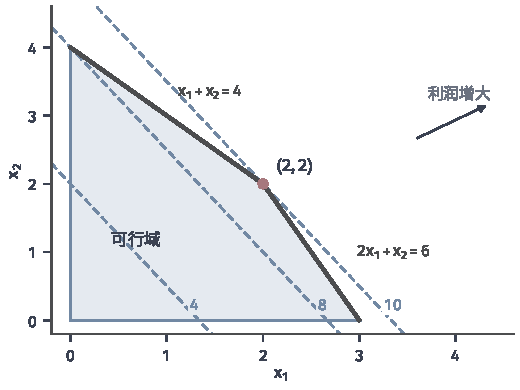
\includegraphics[width=88mm]{figures/05-optimization/01-linear-programming/matplotlib/opt-resource-region/figure.pdf}
  \caption{资源分配问题。浅蓝色四边形是全部允许的产量组合，顶点为$(0,0),(3,0),(2,2),(0,4)$；深灰粗线是工时约束与原料约束的边界。蓝色虚线是利润等于$4,8,10$的直线，红点$(2,2)$是利润为$10$的线与四边形唯一的公共点。}
  \label{fig:opt-resource-region}
\end{BookInlineFigure}

\paragraph{二次拟合}
第二个任务来自数据。设有$N$个观测和$n$个待定系数，矩阵$\bm{A}\in\mathbb{R}^{N\times n}$的第$i$行记录第$i$个观测的输入，向量$\bm{b}\in\mathbb{R}^N$记录观测值。系数$\bm{x}\in\mathbb{R}^n$给出的预测是$\bm{A}\bm{x}$，我们用平方误差比较不同的系数：
\begin{equation}
 f(\bm{x})=\frac12\lVert\bm{A}\bm{x}-\bm{b}\rVert_2^2+\frac{\gamma}{2}\lVert\bm{x}\rVert_2^2,\qquad\gamma\geq0.
 \label{eq:opt-ridge}
\end{equation}
第一项衡量预测与观测的差距，第二项称为正则项，系数$\gamma$决定对大系数收多少“费”。这个目标是$\bm{x}$的二次函数，所以称为二次拟合。

全章反复使用一个最小的实例：只有一个观测，$N=1$；两个系数，$n=2$；$\bm{A}=(1\ \ 1)$，$\bm{b}=2$。它的含义是“只测到两个量的和约等于$2$”。此时
\begin{equation}
 f(\bm{x})=\frac12(x_1+x_2-2)^2+\frac{\gamma}{2}(x_1^2+x_2^2).
 \label{eq:opt-ridge-instance}
\end{equation}
这个例子小到可以手算，却已经包含解不唯一、平坦方向和误差指标互相矛盾这些现象。

\paragraph{统一的写法}
两个任务都是在一个集合里选$\bm{x}$，使一个数尽量小。我们把这个结构固定下来，并同时规定全卷的记号。

\begin{definition}[优化问题]
\label{def:opt-problem}
给定集合$\bm{C}\subseteq\mathbb{R}^n$与函数$f:\bm{C}\to\mathbb{R}$，寻找使$f$尽量小的$\bm{x}\in\bm{C}$的任务称为\term{优化问题}（optimization problem），写作
\begin{equation}
 \min_{\bm{x}\in\bm{C}}f(\bm{x}).
 \label{eq:opt-general}
\end{equation}
$\bm{x}$称为\term{决策变量}（decision variable），$f$称为\term{目标函数}（objective function），$\bm{C}$称为\term{可行集}（feasible set），$\bm{C}$中的点称为\term{可行点}（feasible point）。
\end{definition}

可行集常常由一组条件给出。全卷把不等式都整理成“$\leq0$”的形式，写作
\begin{equation}
 \bm{C}=\bigl\{\bm{x}\in\mathbb{R}^n:\ g_i(\bm{x})\leq0,\ i=1,\ldots,m;\ h_j(\bm{x})=0,\ j=1,\ldots,p\bigr\}.
 \label{eq:opt-constraint-form}
\end{equation}
其中$g_i$是不等式约束，共$m$个；$h_j$是等式约束，共$p$个。资源分配里没有等式约束，四个不等式约束是
\[
 g_1(\bm{x})=x_1+x_2-4,\quad g_2(\bm{x})=2x_1+x_2-6,\quad g_3(\bm{x})=-x_1,\quad g_4(\bm{x})=-x_2.
\]
二次拟合里没有约束，$\bm{C}=\mathbb{R}^n$。

$\bm{C}$与$f$必须一起给定，问题才算确定。对二次拟合而言，改变$\gamma$是在改变候选之间的比较标准，全部候选都还在；加上硬性要求$x_1\geq1.2$则是把一部分候选直接淘汰。前者像调整评分表，后者像修改参赛资格。两种改动都可能让答案变化，但机制不同，这一区别到本节末尾还会出现。

\paragraph{最优值与最优解}
“最低点”其实包含两个问题：最低的高度是多少，这个高度在哪里取得。前者是一个数，后者是一个位置。两者要分开定义，因为第一个问题有答案时，第二个问题可能没有。

\begin{definition}[最优值与最优解]
\label{def:opt-optimal-value}
问题~\eqref{eq:opt-general}的\term{最优值}（optimal value）是
\begin{equation}
 f^\star=\inf_{\bm{x}\in\bm{C}}f(\bm{x})\in[-\infty,+\infty],
 \label{eq:opt-optimal-value}
\end{equation}
并约定空集上的下确界为$+\infty$。若可行点$\bm{x}^\star$满足$f(\bm{x}^\star)=f^\star$，就称它为\term{最优解}（optimal solution）。全体最优解组成的集合记为$\argmin_{\bm{x}\in\bm{C}}f(\bm{x})$。这个集合非空时，称最优值被达到。
\end{definition}

符号$\min$在式~\eqref{eq:opt-general}中只表示提出任务。若有人写“最小值等于某个数”，他同时断言了这个数被某个可行点取得；若只知道下确界，应当写$\inf$。

现在解资源分配问题。要证明$(2,2)$最好，需要两件事：所有可行点的利润都不超过某个数，并且$(2,2)$达到了这个数。第一件事可以这样做：利润系数$(3,2)$恰好是两条资源约束系数$(1,1)$与$(2,1)$之和，所以对任意可行点，把两条约束相加，得到
\[
 3x_1+2x_2=(x_1+x_2)+(2x_1+x_2)\leq4+6=10.
\]

这说明$f(\bm{x})\geq-10$对所有可行点成立。等号成立当且仅当两条资源约束同时取等号，也就是
\[
 x_1+x_2=4,\qquad 2x_1+x_2=6.
\]
解得$\bm{x}=(2,2)$，它满足非负约束，因而可行。于是
\[
 f^\star=-10,\qquad \argmin_{\bm{x}\in\bm{C}}f(\bm{x})=\{(2,2)\}.
\]

这个论证的结构值得记住：一个对所有可行点成立的下界，加上一个达到该下界的可行点，从两侧把最优值夹住，两者缺一不可。只有下界，不知道它是否够紧；只有候选点，不知道还有没有更好的。第~\ref{chap:linear-programming}章会说明，“给约束配权重再相加”可以系统地做。

二次拟合实例~\eqref{eq:opt-ridge-instance}取$\gamma=0$时，$f(\bm{x})=\frac12(x_1+x_2-2)^2\geq0$。凡满足$x_1+x_2=2$的点都使$f=0$，所以$f^\star=0$，最优解是一整条直线。比如$(1,1)$和$(3,-1)$都最优。数据只约束了两个量的和，没有约束它们的差，参数不唯一并不是计算失败，而是问题本身没有提供区分它们的信息。

\paragraph{三种没有最优解的情形}
并不是每个问题都有解，失败有三种不同的方式，分别出在不同的环节。

\begin{itemize}
 \item \term{不可行}（infeasible）：$\bm{C}=\varnothing$，此时$f^\star=+\infty$。例如同时要求$x\leq0$与$x\geq1$。
 \item \term{无下界}（unbounded below）：$\bm{C}\neq\varnothing$且$f^\star=-\infty$。例如在$\mathbb{R}$上最小化$f(x)=x$，取$x=-k$可得$f=-k\to-\infty$。
 \item 下确界未达到：$f^\star$是有限实数，但$\argmin$为空。例如在$\mathbb{R}$上最小化$f(x)=e^x$。
\end{itemize}

第三种最容易被忽略。对$e^x$，处处有$e^x>0$，又有$e^{-k}\to0$，所以$f^\star=0$；但没有$x$使$e^x=0$。只报告“最优值是$0$”而不说明它未被达到，读者会以为存在一个最优的$x$。图~\ref{fig:opt-failure-modes}把三种情形放在一起。

\begin{BookInlineFigure}
  \centering
  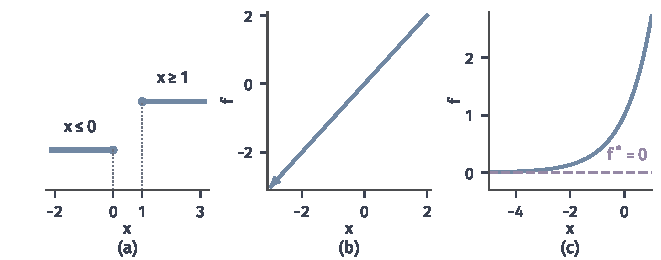
\includegraphics[width=112mm]{figures/05-optimization/01-linear-programming/matplotlib/opt-failure-modes/figure.pdf}
  \caption{优化问题没有最优解的三种方式。(a)约束$x\leq0$与$x\geq1$对应的两段蓝色射线没有公共点，可行集为空。(b)$f(x)=x$沿箭头方向无限下降，最优值为$-\infty$。(c)$f(x)=e^x$趋于紫色虚线$f^\star=0$却永远碰不到：最优值有限，但没有点取得它。}
  \label{fig:opt-failure-modes}
\end{BookInlineFigure}

\paragraph{局部最优与全局最优}
前面的最优解要和所有可行点比。实际计算时，我们往往只看得见当前点附近的情况，所以还需要一个只和附近比较的概念。“附近”用开球表示：
\[
 \bm{B}(\bm{x},r)=\{\bm{y}:\lVert\bm{y}-\bm{x}\rVert_2<r\}.
\]

\begin{definition}[局部最优解]
\label{def:opt-local}
设$\bm{x}^\star\in\bm{C}$。若存在$r>0$，使
\begin{equation}
 f(\bm{x}^\star)\leq f(\bm{x})\qquad\text{对所有}\ \bm{x}\in\bm{C}\cap\bm{B}(\bm{x}^\star,r)\ \text{成立},
 \label{eq:opt-local}
\end{equation}
就称$\bm{x}^\star$为\term{局部最优解}（local minimizer）。若对其中所有$\bm{x}\neq\bm{x}^\star$都有严格不等式，就称它为\term{严格局部最优解}（strict local minimizer）。定义~\ref{def:opt-optimal-value}中的最优解也称\term{全局最优解}（global minimizer）。
\end{definition}

比较的范围是$\bm{C}\cap\bm{B}(\bm{x}^\star,r)$，不是整个球。可行集边界上的点只需要和球内的可行点比较，球里伸出可行集的部分不参加比较。下面的例子同时展示洼地与边界。

\begin{example}[两个洼地与一个边界]
\label{ex:opt-local-global}
在可行集$\bm{C}=[-1.5,1.5]$上最小化
\[
 f(x)=\frac{x^4}{4}-\frac{x^3}{3}-x^2.
\]
先求导并分解因式：
\[
 f'(x)=x^3-x^2-2x=x(x-2)(x+1).
\]
所以$f'$在$x=-1,0,2$处为零。其中$x=2$在可行集之外。由$f'$的符号，$f$在$[-1.5,-1]$上递减，在$[-1,0]$上递增，在$[0,1.5]$上递减。

因此$x=-1$附近的可行点函数值都不低于$f(-1)$，它是局部最优解。$\bm{C}$上的最小值只可能出现在$x=-1$或右端点$x=1.5$，两处的函数值是
\[
 f(-1)=-\frac{5}{12}\approx-0.417,\qquad f(1.5)\approx-2.109.
\]
所以全局最优解是$x=1.5$。这一点在边界上，那里$f'(1.5)=-1.875\neq0$：函数还在向右下降，只是可行集不允许再往右走。
\end{example}

图~\ref{fig:opt-local-global}画出这个例子，地形的比喻在这里很贴切。黄点是一个洼地的底部，站在那里四周都更高，它却不是最低处。红点是真正的最低处，脚下的地面还是斜的，挡住我们的是边界，不是地形。可行集右侧还有更低的点$x=2$，但它不是候选，与问题无关。

\begin{BookInlineFigure}
  \centering
  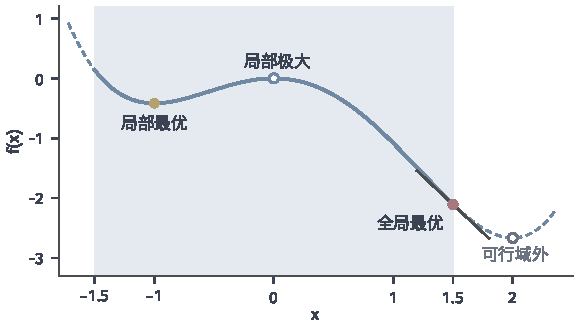
\includegraphics[width=98mm]{figures/05-optimization/01-linear-programming/matplotlib/opt-local-global/figure.pdf}
  \caption{$f(x)=x^4/4-x^3/3-x^2$在$\bm{C}=[-1.5,1.5]$（浅蓝色带）上的局部与全局最优。蓝色实线是$\bm{C}$上的图像，虚线是$\bm{C}$外的部分。黄点$x=-1$是局部最优解，红点$x=1.5$是全局最优解，该处的短切线不水平，斜率为$-1.875$。空心点分别是局部极大点$x=0$和可行集外的$x=2$。}
  \label{fig:opt-local-global}
\end{BookInlineFigure}

严格局部最优只说明一个小邻域内没有并列者，并不排除远处有同样低的点。函数$(x^2-1)^2$在$x=\pm1$处都取到全局最小值$0$，两点各自是严格局部最优解，全局最优解却有两个。

\paragraph{把约束并入目标}
到目前为止，可行集和目标是两个分开的对象。后面常要把几种代价相加，或者用同一个工具处理各种约束，分开写很不方便。一个自然的想法是：给不可行的点一个大到不可能被选中的值。任何有限的数都不够保险，所以我们允许函数取$+\infty$。

\begin{definition}[扩展实值函数与约束指标函数]
\label{def:opt-extended}
取值于$\mathbb{R}\cup\{+\infty\}$的函数称为\term{扩展实值函数}（extended real-valued function）。它的\term{有效定义域}（effective domain）是$\operatorname{dom}F=\{\bm{x}:F(\bm{x})<+\infty\}$；有效定义域非空时，称$F$为\term{适当函数}（proper function）。集合$\bm{C}\subseteq\mathbb{R}^n$的\term{约束指标函数}（constraint indicator function）是
\begin{equation}
 \iota_{\bm{C}}(\bm{x})=\begin{cases}0,&\bm{x}\in\bm{C},\\+\infty,&\bm{x}\notin\bm{C}.\end{cases}
 \label{eq:opt-constraint-indicator}
\end{equation}
扩展实值目标$F$的最优解集合规定为
\begin{equation}
 \argmin F=\{\bm{x}\in\operatorname{dom}F:F(\bm{x})=\inf F\}.
 \label{eq:opt-extended-argmin}
\end{equation}
\end{definition}

对可行集$\bm{C}$非空的问题，令$F=f+\iota_{\bm{C}}$，也就是在$\bm{C}$上$F=f$，在$\bm{C}$外$F=+\infty$。这里$f+\iota_{\bm{C}}$在$\bm{C}$外按$+\infty$理解，不要求$f$在那里有定义。逐项核对这种写法保留了什么。

首先，$\operatorname{dom}F=\bm{C}$，所以取有限值的候选恰好是可行点。其次，$F$与$f$在可行点上取值相同，其余点取$+\infty$，不影响下确界，于是
\[
 \inf_{\mathbb{R}^n}F=\inf_{\bm{x}\in\bm{C}}f(\bm{x}).
\]
最后，最优解只在$\operatorname{dom}F=\bm{C}$中找，所以$\argmin F$与原问题的最优解集合相同。若$\bm{C}=\varnothing$，则$F\equiv+\infty$不是适当函数，应报告不可行；定义中限定在$\operatorname{dom}F$内找解，正是为了避免说成“每一点都最优”。

\paragraph{约束指标函数不是普通指示函数}
名称相近的普通\term{指示函数}（indicator function）$\mathbb{1}_{\bm{C}}$在$\bm{C}$上取$1$，在$\bm{C}$外取$0$。两者的取值表放在一起，就能看出差别。

\begin{BookInlineTable}
  \centering
  \begin{tabular}{@{}lcc@{}}
    \toprule
     & $\bm{x}\in\bm{C}$ & $\bm{x}\notin\bm{C}$\\
    \midrule
    约束指标函数$\iota_{\bm{C}}$ & $0$ & $+\infty$\\
    普通指示函数$\mathbb{1}_{\bm{C}}$ & $1$ & $0$\\
    \bottomrule
  \end{tabular}
  \caption{约束指标函数与普通指示函数的取值。前者用于把违规点排除，后者只是记录一个点是否属于集合。}
  \label{tab:opt-indicators}
\end{BookInlineTable}

两者的方向也相反：$\iota_{\bm{C}}$在集合内为小值，$\mathbb{1}_{\bm{C}}$在集合内为大值。用一个例子看把它们加到目标上的后果。在约束$x\leq1$下最小化$(x-2)^2$，可行集记为$C=(-\infty,1]$。这个问题的最优解是$x=1$，最优值为$1$。

图~\ref{fig:opt-extended-value}比较三种加法。加$\iota_C$得到的问题就是原问题。加$\mathbb{1}_C$则让可行点反而贵了$1$，最小点跑到$x=2$，违反约束。

第三种是有限惩罚，它按违规程度收费。改为最小化$(x-2)^2+\max\{0,x-1\}$，在$x>1$的范围内令导数为零：
\[
 2(x-2)+1=0,\qquad x=1.5.
\]
此处函数值是$0.25+0.5=0.75$，低于约束问题的最优值$1$，所以惩罚问题的最小点违反了约束。

\begin{BookInlineFigure}
  \centering
  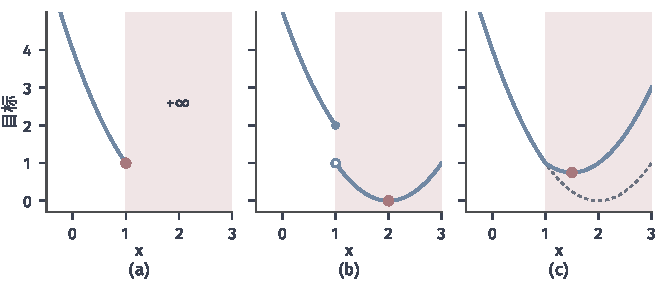
\includegraphics[width=112mm]{figures/05-optimization/01-linear-programming/matplotlib/opt-extended-value/figure.pdf}
  \caption{把约束$x\leq1$并入目标$(x-2)^2$的三种做法，浅红区域是不可行的点，红点是所得问题的最小点。(a)加约束指标函数，浅红区域取$+\infty$，最小点$x=1$与原问题相同。(b)加普通指示函数，可行点上升$1$，最小点变成不可行的$x=2$。(c)加有限惩罚$\max\{0,x-1\}$（灰色点线是原目标），最小点$x=1.5$仍不可行。}
  \label{fig:opt-extended-value}
\end{BookInlineFigure}

约束指标函数只是把同一个问题换了写法；有限惩罚改变了问题，只是不喜欢违规，并不禁止违规。惩罚要多大才能恢复约束，是第~\ref{chap:penalty-multiplier-methods}章的话题。今后需要时，我们把约束问题~\eqref{eq:opt-general}直接写成扩展实值目标的最小化，两种写法描述同一个问题。

\section{最优解的存在}
\label{sec:opt-existence}

$e^x$的例子说明，最优值有限并不保证有点取得它。于是要问：在什么条件下，可以不解问题就断定最优解存在？这个问题值得先回答。若解根本不存在，算法再怎么迭代也找不到它，“收敛”二字也就无从谈起。

\paragraph{从越来越好的候选出发}
设$\bm{C}$非空。按下确界的定义，总能取到一列可行点，使目标值趋于$f^\star$。若$f^\star$有限，就对每个$k$取可行点$\bm{x}^{(k)}$，使$f(\bm{x}^{(k)})\leq f^\star+1/k$；若$f^\star=-\infty$，就取$f(\bm{x}^{(k)})\leq-k$。这样的序列称为\term{最小化序列}（minimizing sequence）。上标$(k)$只是序列编号，这里还没有任何算法。

最小化序列的目标值越来越接近最优值，但序列本身可能乱跑。要从它得到一个最优解，需要依次通过三关：

\begin{enumerate}
 \item 序列留得住：存在收敛的子列，候选不会四散或逃向无穷远；
 \item 极限合法：子列的极限仍然是可行点；
 \item 比较能传到极限：极限处的目标值不高于序列目标值的极限。
\end{enumerate}

前两关由可行集负责，第三关由目标函数负责。图~\ref{fig:opt-existence-failures}中的三个例子各拆掉一关，绿点是最小化序列。

\begin{BookInlineFigure}
  \centering
  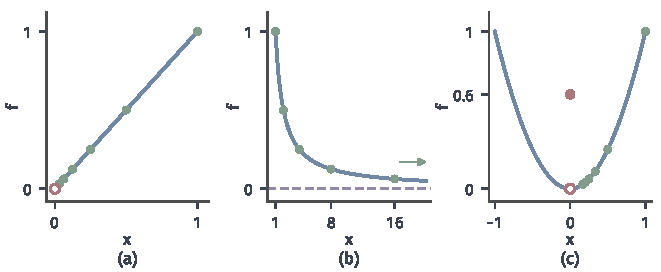
\includegraphics[width=112mm]{figures/05-optimization/01-linear-programming/matplotlib/opt-existence-failures/figure.pdf}
  \caption{存在性论证的三关分别失败。绿点是最小化序列。(a)$f(x)=x$，$C=(0,1]$：序列$2^{-k}$趋于不可行的端点$0$（红色空心点）。(b)$f(x)=1/x$，$C=[1,\infty)$：序列$2^k$逃向无穷远，目标值趋于紫色虚线$0$。(c)$f(x)=x^2$（$x\neq0$），$f(0)=0.6$，$C=[-1,1]$：序列$1/k$趋于$0$，目标值趋于$0$，而$f(0)$跳高到红点$0.6$，值$0$无人取得。}
  \label{fig:opt-existence-failures}
\end{BookInlineFigure}

(a)中$C=(0,1]$有界但不闭，序列有极限$0$，极限却被排除在外，第二关失败。(b)中$C=[1,\infty)$闭但无界，序列$2^k$没有收敛子列，第一关失败。(c)中$C=[-1,1]$很好，序列也收敛到可行点$0$，但函数在$0$处向上跳，极限处的值$0.6$高于序列目标值的极限$0$，第三关失败。

\paragraph{第一关与第二关：紧性}
在$\mathbb{R}^n$中，有界闭集的每个序列都有收敛子列，而且子列的极限仍在集合内。这样的集合称为\term{紧集}（compact set）。紧性恰好一次通过前两关：有界让序列留得住，闭让极限合法。有界闭集的这一性质及一般度量空间中的紧致性，可参考\BookChapterRef{chap:metric-spaces}{卷四第2章“度量空间”}。

\paragraph{第三关：只需要单向的比较}
第三关若用连续性通过，得到的是熟悉的结论：有界闭集上的连续函数取得最小值。仔细看却会发现，连续性要求多了。我们只需要极限处的值“不比序列高”，不需要它“等于序列的极限”。函数在极限点向下跳，只会让极限点更好；不能允许的是向上跳。

\begin{definition}[下半连续]
\label{def:opt-lsc}
设$\bm{C}\subseteq\mathbb{R}^n$，$f:\bm{C}\to\mathbb{R}\cup\{+\infty\}$。若对$\bm{C}$中每个收敛到$\bm{x}\in\bm{C}$的序列$\bm{x}^{(k)}$，都有
\begin{equation}
 f(\bm{x})\leq\liminf_{k\to\infty}f(\bm{x}^{(k)}),
 \label{eq:opt-lsc}
\end{equation}
就称$f$在$\bm{C}$上\term{下半连续}（lower semicontinuous）。
\end{definition}

连续函数满足这个条件且取等号。下半连续还可以用“高度不超过某个水平的部分”来刻画。对实数$a$，称
\begin{equation}
 \bm{S}_a=\{\bm{x}\in\bm{C}:f(\bm{x})\leq a\}
 \label{eq:opt-sublevel}
\end{equation}
为$f$的\term{下水平集}（sublevel set），也就是地形图上高度不超过$a$的区域。

图~\ref{fig:opt-lsc-sublevel}比较两个只在$x=0$一点取值不同的函数。左边$f(0)=0.4$，取跳跃下方的值，下半连续，高度不超过$0.6$的点组成闭区间$[0,0.4]$。右边$f(0)=1$，取跳跃上方的值，不下半连续，同一个下水平集是$(0,0.4]$，缺了左端点。右边的函数沿$x\downarrow0$可以无限接近$0.4$，却被$x=0$处的跳高挡住，最小值取不到。

\begin{BookInlineFigure}
  \centering
  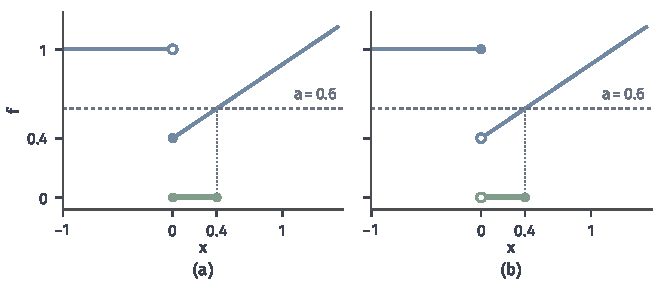
\includegraphics[width=112mm]{figures/05-optimization/01-linear-programming/matplotlib/opt-lsc-sublevel/figure.pdf}
  \caption{下半连续与下水平集的缺口。两个函数在$x<0$时都等于$1$，在$x>0$时都等于$0.4+0.5x$，实心蓝点是$x=0$处的函数值。灰色点线是水平$a=0.6$，绿色线段是下水平集$\bm{S}_{0.6}$。(a)$f(0)=0.4$，下半连续，下水平集是闭区间$[0,0.4]$。(b)$f(0)=1$，向上跳，下水平集$(0,0.4]$缺少左端点。}
  \label{fig:opt-lsc-sublevel}
\end{BookInlineFigure}

图中的观察就是下面的引理：下半连续性的作用，是让下水平集不缺边界。

\begin{lemma}[下半连续与闭下水平集]
\label{lem:opt-lsc-sublevel}
设$\bm{C}\subseteq\mathbb{R}^n$是闭集，$f:\bm{C}\to\mathbb{R}\cup\{+\infty\}$。$f$在$\bm{C}$上下半连续，当且仅当对每个$a\in\mathbb{R}$，下水平集$\bm{S}_a$是闭集。
\end{lemma}

\begin{proof}
先设$f$下半连续。取$\bm{S}_a$中的序列$\bm{x}^{(k)}$，设它收敛到$\bm{x}$。$\bm{C}$是闭集，所以$\bm{x}\in\bm{C}$。由下半连续性，
\[
 f(\bm{x})\leq\liminf_{k\to\infty}f(\bm{x}^{(k)})\leq a.
\]
所以$\bm{x}\in\bm{S}_a$，$\bm{S}_a$是闭集。

反过来，设每个$\bm{S}_a$都是闭集，但$f$在某点$\bm{x}\in\bm{C}$不满足式~\eqref{eq:opt-lsc}，即存在$\bm{C}$中收敛到$\bm{x}$的序列，使$\liminf_kf(\bm{x}^{(k)})<f(\bm{x})$。取实数$a$严格介于这两个量之间。下极限小于$a$，所以有子列$\bm{x}^{(k_j)}$始终满足$f(\bm{x}^{(k_j)})\leq a$，也就是子列落在$\bm{S}_a$中。

$\bm{S}_a$是闭集，子列的极限$\bm{x}$也在其中，于是$f(\bm{x})\leq a$。这与$a<f(\bm{x})$矛盾。
\end{proof}

\paragraph{紧可行集上的存在定理}
三关齐备，就得到第一个存在定理。

\begin{theorem}[紧可行集上的最小值]
\label{thm:opt-compact-existence}
设$\bm{C}\subseteq\mathbb{R}^n$非空且紧，$f:\bm{C}\to\mathbb{R}\cup\{+\infty\}$在$\bm{C}$上下半连续，且至少有一点取有限值。则最优值$f^\star$是有限实数，且最优解存在。
\end{theorem}

\begin{proof}
由假设，$f^\star<+\infty$。取一个最小化序列$\bm{x}^{(k)}\in\bm{C}$。$\bm{C}$是紧集，所以有子列$\bm{x}^{(k_j)}$收敛到某个$\bm{x}^\star\in\bm{C}$。由下半连续性，
\[
 f(\bm{x}^\star)\leq\liminf_{j\to\infty}f(\bm{x}^{(k_j)})=f^\star.
\]

若$f^\star=-\infty$，上式给出$f(\bm{x}^\star)=-\infty$，与$f$不取$-\infty$矛盾，所以$f^\star$有限。又因$\bm{x}^\star$可行，有$f(\bm{x}^\star)\geq f^\star$。两个不等式合起来得到
\[
 f(\bm{x}^\star)=f^\star.
\]
所以$\bm{x}^\star$是最优解。
\end{proof}

资源分配的可行集由四个闭半平面相交而成，它有界且闭，目标是线性函数，因而连续。定理~\ref{thm:opt-compact-existence}立刻保证最优解存在。这个结论不需要知道解在$(2,2)$，它只告诉我们值得去找。

定理的条件都是充分条件。例如$f(x)=x^2$的可行集$\mathbb{R}$无界，最小点$x=0$依然存在。图~\ref{fig:opt-existence-failures}的三个例子说明的是：逐条去掉条件后，结论可能不成立。

\paragraph{无界可行集：只看不太差的点}
二次拟合的可行集是整个$\mathbb{R}^n$，它不紧，定理~\ref{thm:opt-compact-existence}不能直接用。但我们并不需要整个可行集紧，只需要把最小化序列关进某个紧集。取一个有限的水平$a$，使下水平集$\bm{S}_a$非空。凡是目标值高于$a$的点都比$\bm{S}_a$中的点差，不可能是最优解，可以直接丢掉。剩下要看的只有$\bm{S}_a$。

\begin{theorem}[紧下水平集保证存在]
\label{thm:opt-compact-sublevel}
设$f:\bm{C}\to\mathbb{R}\cup\{+\infty\}$在$\bm{C}$上下半连续。若存在实数$a$，使下水平集$\bm{S}_a$非空且紧，则$f^\star$是有限实数，且最优解存在。
\end{theorem}

\begin{proof}
$f$限制在紧集$\bm{S}_a$上仍下半连续，并在$\bm{S}_a$上取有限值。由定理~\ref{thm:opt-compact-existence}，存在$\bm{x}^\star\in\bm{S}_a$，使$f(\bm{x}^\star)=\min_{\bm{S}_a}f\leq a$。

对$\bm{C}\setminus\bm{S}_a$中的点，有$f(\bm{x})>a\geq f(\bm{x}^\star)$。所以$\bm{x}^\star$是$f$在整个$\bm{C}$上的最小点，$f^\star=f(\bm{x}^\star)$有限。
\end{proof}

这个定理只要求有一个下水平集紧，其余的下水平集可以无界。在$\mathbb{R}$上考虑
\[
 f(x)=\frac{x^2}{1+x^2}.
\]
令$a=1/2$，解不等式$f(x)\leq1/2$，得到$x^2\leq1$，所以$\bm{S}_{1/2}=[-1,1]$是紧集，最小点$x=0$由此得到保证。而取$a\geq1$时，下水平集是整个$\mathbb{R}$，无界。

怎样检验下水平集紧？闭性由引理~\ref{lem:opt-lsc-sublevel}给出，只要$\bm{C}$闭、$f$下半连续。有界性则需要目标在远处足够高，这就是强制性。

\begin{definition}[强制性]
\label{def:opt-coercive}
设$\bm{C}\subseteq\mathbb{R}^n$，$f:\bm{C}\to\mathbb{R}\cup\{+\infty\}$。若对$\bm{C}$中任意满足$\lVert\bm{x}^{(k)}\rVert_2\to\infty$的序列，都有$f(\bm{x}^{(k)})\to+\infty$，就称$f$在$\bm{C}$上是\term{强制的}（coercive）。
\end{definition}

强制性等价于每个下水平集都有界。若某个$\bm{S}_a$无界，从中取范数趋于无穷的序列，其目标值始终不超过$a$，不满足强制性。反过来，若各下水平集都有界，而$\lVert\bm{x}^{(k)}\rVert_2\to\infty$，则对任意$a$，序列最终离开$\bm{S}_a$，也就是最终$f(\bm{x}^{(k)})>a$，所以$f(\bm{x}^{(k)})\to+\infty$。

于是得到实际最常用的形式：若$\bm{C}$非空闭，$f$下半连续且强制，并在$\bm{C}$上至少有一点取有限值，则最优解存在。这只需取$a$为该点的函数值，再用定理~\ref{thm:opt-compact-sublevel}。各条件的分工是：强制性使下水平集有界，留住了序列；$\bm{C}$闭与下半连续使下水平集闭，留住了极限。

\paragraph{回到二次拟合}
对式~\eqref{eq:opt-ridge}逐项核对。$f$是多项式，处处有限且连续；$\bm{C}=\mathbb{R}^n$是闭集。当$\gamma>0$时，拟合项非负，所以
\[
 f(\bm{x})\geq\frac{\gamma}{2}\lVert\bm{x}\rVert_2^2.
\]
范数趋于无穷时目标趋于无穷，$f$强制，最优解存在。

$\gamma=0$时情况不同。对实例~\eqref{eq:opt-ridge-instance}，沿方向$(1,-1)$目标不变：取$\bm{x}^{(k)}=(1+k,1-k)$，范数趋于无穷而$f=0$，所以$f$不强制。图~\ref{fig:opt-coercive-sublevel}比较了两种情形，同一个水平$a=1$的下水平集，在$\gamma=0$时是无界的带，在$\gamma=0.5$时收缩成一个椭圆。

\begin{BookInlineFigure}
  \centering
  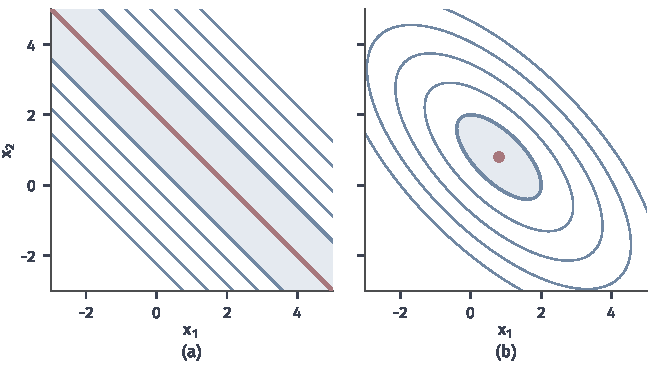
\includegraphics[width=112mm]{figures/05-optimization/01-linear-programming/matplotlib/opt-coercive-sublevel/figure.pdf}
  \caption{二次拟合实例$f(\bm{x})=\frac12(x_1+x_2-2)^2+\frac{\gamma}{2}\lVert\bm{x}\rVert_2^2$的下水平集。浅蓝区域及其粗边界是$\{f\leq1\}$，细线是其他等高线。(a)$\gamma=0$：下水平集是两条平行线之间的无界带，红线$x_1+x_2=2$是最优解集合。(b)$\gamma=0.5$：下水平集是椭圆，红点是唯一最优解$(0.8,0.8)$。}
  \label{fig:opt-coercive-sublevel}
\end{BookInlineFigure}

然而$\gamma=0$时最优解仍然存在，整条直线$x_1+x_2=2$都是。这再次说明强制性只是充分条件。对一般的$\bm{A}$，不带正则项的最小二乘总有解，依据是正规方程$\bm{A}^\top\bm{A}\bm{x}=\bm{A}^\top\bm{b}$总可解，可参考\BookChapterRef{chap:linear-solution-selection}{卷二第11章“线性方程与最小二乘的选解”}，这里用不到强制性。

\paragraph{有限维的边界}
整个论证依赖“有界闭集紧”，这是有限维空间的性质。平方可和的数列空间中，第$k$个坐标为$1$、其余为$0$的数列组成一列单位向量，它们两两距离都是$\sqrt2$，都在闭单位球里，却没有收敛子列。函数空间上的存在性要换一种收敛概念，第~\ref{chap:functional-optimization-variation}章会处理这件事；在$\mathbb{R}^n$中，本节的定理已经够用。

\section{解的性质}
\label{sec:opt-properties}

知道解存在之后，自然要问这个解是什么样的：洼地的底部是不是最低处？最低点是不是只有一个？目标值接近最优时，位置也接近吗？这些问题都在比较两个候选，最简单的比较路径是连接它们的线段。本节一路沿线段比较，逐步加强要求，依次回答这三个问题。

\paragraph{凸集：线段留在里面}
资源分配中，方案$\bm{u}=(3,0)$与$\bm{v}=(0,4)$都可行。各执行一半，得到混合方案$\frac12\bm{u}+\frac12\bm{v}=(1.5,2)$，它也可行，因为$1.5+2=3.5\leq4$，$3+2=5\leq6$，产量也非负。

这不是巧合。若$\bm{u},\bm{v}$都满足同一个线性不等式$\langle\bm{a},\bm{x}\rangle\leq c$，则对$\theta\in[0,1]$，
\[
 \langle\bm{a},\theta\bm{u}+(1-\theta)\bm{v}\rangle
 =\theta\langle\bm{a},\bm{u}\rangle+(1-\theta)\langle\bm{a},\bm{v}\rangle
 \leq\theta c+(1-\theta)c=c.
\]
可行方案任意混合仍然可行，这个性质值得单独命名。

\begin{definition}[凸集]
\label{def:opt-convex-set}
若对任意$\bm{u},\bm{v}\in\bm{C}$与$\theta\in[0,1]$，都有
\begin{equation}
 \theta\bm{u}+(1-\theta)\bm{v}\in\bm{C},
 \label{eq:opt-convex-set}
\end{equation}
就称$\bm{C}\subseteq\mathbb{R}^n$为\term{凸集}（convex set）。
\end{definition}

几何上，凸集里任意两点之间的线段都留在集合内。上面的计算说明半空间$\{\bm{x}:\langle\bm{a},\bm{x}\rangle\leq c\}$是凸集。若干凸集的交仍是凸集：两点同时在每个集合中，线段也同时在每个集合中。资源分配的可行集是四个半空间的交，所以是凸集。图~\ref{fig:opt-convex-sets}给出对照。

\begin{BookInlineFigure}
  \centering
  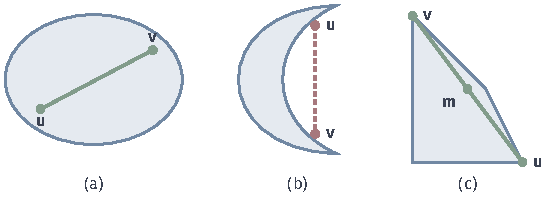
\includegraphics[width=93.691mm]{figures/05-optimization/01-linear-programming/tikz/opt-convex-sets/figure.pdf}
  \caption{凸集与非凸集。(a)椭圆盘中任意两点间的绿色线段留在集合内。(b)月牙形中两点都在集合里，红色虚线却穿过缺口，所以不是凸集。(c)资源分配的可行四边形，$\bm{u}=(3,0)$与$\bm{v}=(0,4)$的等权混合$\bm{m}=(1.5,2)$仍在集合内。}
  \label{fig:opt-convex-sets}
\end{BookInlineFigure}

\paragraph{凸函数：图像不鼓过弦}
可行集凸时，两个可行点之间的线段全是候选。接下来要求目标沿这条线段“不鼓起来”：线段上每一点的目标值，不超过两端目标值按相同权重的平均。

\begin{definition}[凸函数]
\label{def:opt-convex-function}
设$\bm{C}$为凸集。若$f:\bm{C}\to\mathbb{R}$对任意$\bm{u},\bm{v}\in\bm{C}$与$\theta\in[0,1]$满足
\begin{equation}
 f\bigl(\theta\bm{u}+(1-\theta)\bm{v}\bigr)\leq\theta f(\bm{u})+(1-\theta)f(\bm{v}),
 \label{eq:opt-convex-function}
\end{equation}
就称$f$为$\bm{C}$上的\term{凸函数}（convex function）。扩展实值函数称为凸函数，是指其有效定义域为凸集，且式~\eqref{eq:opt-convex-function}对有效定义域中的点成立。
\end{definition}

式~\eqref{eq:opt-convex-function}右端是连接两点$(\bm{u},f(\bm{u}))$与$(\bm{v},f(\bm{v}))$的弦上的点，左端是同一位置的函数值。所以凸函数的图像位于每条弦的下方，也就是碗的形状。图~\ref{fig:opt-chord}(a)是凸函数$x^2/2$；(b)中的函数有两个碗，连接两侧的弦从中间的鼓包下面穿过，不等式被破坏。对$F=f+\iota_{\bm{C}}$，这个定义恰好要求$\bm{C}$凸且$f$在$\bm{C}$上凸。

\begin{BookInlineFigure}
  \centering
  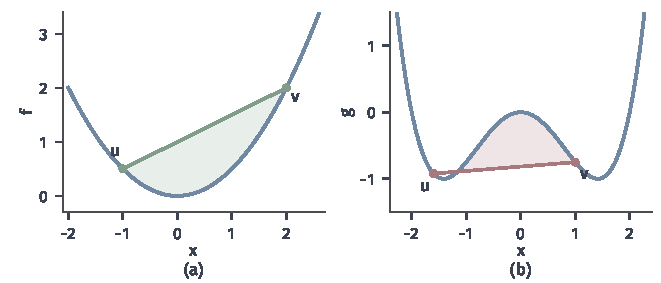
\includegraphics[width=112mm]{figures/05-optimization/01-linear-programming/matplotlib/opt-chord/figure.pdf}
  \caption{图像与弦。(a)凸函数$f(x)=x^2/2$，连接$x=-1$与$x=2$的绿色弦位于图像上方，浅绿区域是两者的间隔。(b)非凸函数$g(x)=x^4/4-x^2$，连接$x=-1.6$与$x=1$的红色弦有一段位于图像下方，浅红区域就是违反凸性的部分。}
  \label{fig:opt-chord}
\end{BookInlineFigure}

二次函数的情形可以算到底。设$\bm{H}\in\mathbb{R}^{n\times n}$对称，考虑
\[
 q(\bm{x})=\frac12\bm{x}^\top\bm{H}\bm{x}+\bm{a}^\top\bm{x}+a_0.
\]
记$\bm{w}=\theta\bm{u}+(1-\theta)\bm{v}$，我们计算弦与函数之间的间隔。线性项和常数项在加权平均中抵消，只需展开二次项：
\[
 \bm{w}^\top\bm{H}\bm{w}=\theta^2\bm{u}^\top\bm{H}\bm{u}+2\theta(1-\theta)\bm{u}^\top\bm{H}\bm{v}+(1-\theta)^2\bm{v}^\top\bm{H}\bm{v}.
\]

用$\theta-\theta^2=\theta(1-\theta)$，以及$(1-\theta)-(1-\theta)^2=\theta(1-\theta)$，得到
\begin{equation}
 \theta q(\bm{u})+(1-\theta)q(\bm{v})-q(\bm{w})=\frac12\theta(1-\theta)(\bm{u}-\bm{v})^\top\bm{H}(\bm{u}-\bm{v}).
 \label{eq:opt-quadratic-gap}
\end{equation}
所以$q$凸当且仅当$\bm{H}$半正定。

二次拟合目标~\eqref{eq:opt-ridge}展开后正是这种形式，其中$\bm{H}=\bm{A}^\top\bm{A}+\gamma\bm{I}$。对任意$\bm{w}$，
\[
 \bm{w}^\top\bm{H}\bm{w}=\lVert\bm{A}\bm{w}\rVert_2^2+\gamma\lVert\bm{w}\rVert_2^2\geq0,
\]
所以目标是凸函数。资源分配的目标是线性函数，式~\eqref{eq:opt-convex-function}取等号，也是凸函数。

\paragraph{局部最优就是全局最优}
现在回答第一个问题：山那边会不会有更深的谷。若目标和可行集都是凸的，答案是不会。

\begin{theorem}[凸问题的局部最优是全局最优]
\label{thm:opt-local-global}
设$\bm{C}$为凸集，$f:\bm{C}\to\mathbb{R}$为凸函数。则$f$在$\bm{C}$上的每个局部最优解都是全局最优解，并且最优解集合是凸集。
\end{theorem}

\begin{proof}
设$\bm{u}$是局部最优解，对应的邻域半径为$r$。假设存在$\bm{v}\in\bm{C}$使$f(\bm{v})<f(\bm{u})$。对$t\in(0,1)$，点$\bm{u}+t(\bm{v}-\bm{u})$在线段上，所以属于$\bm{C}$。由式~\eqref{eq:opt-convex-function}，
\[
 f\bigl(\bm{u}+t(\bm{v}-\bm{u})\bigr)\leq(1-t)f(\bm{u})+tf(\bm{v})<f(\bm{u}).
\]

取$t$足够小，使$t\lVert\bm{v}-\bm{u}\rVert_2<r$，这个更低的点就落在$\bm{C}\cap\bm{B}(\bm{u},r)$中，与局部最优矛盾。所以$\bm{u}$是全局最优解。

若$\bm{u},\bm{v}$都是最优解，线段上的点满足$f\leq\theta f^\star+(1-\theta)f^\star=f^\star$，也是最优解，所以最优解集合是凸集。
\end{proof}

证明的几何意义是：如果远处有更低的点，连向它的弦从当前点一出发就下降，凸函数的图像又在弦下方，紧贴当前点就有更低的点。图~\ref{fig:opt-local-implies-global}用非凸的例子~\ref{ex:opt-local-global}反过来看这件事：局部最优点$u$与更低的点$v$之间，弦在$u$的邻域里就低于$f(u)$，而图像却在弦上方，浅红区域正是对凸性的违反。

\begin{BookInlineFigure}
  \centering
  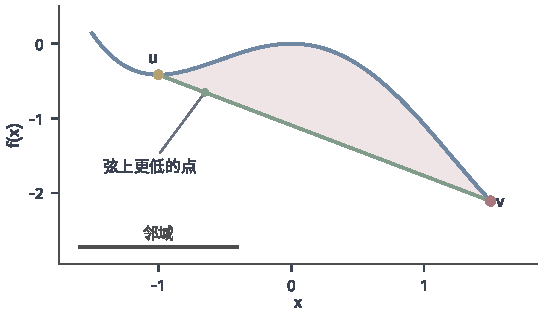
\includegraphics[width=92mm]{figures/05-optimization/01-linear-programming/matplotlib/opt-local-implies-global/figure.pdf}
  \caption{为什么凸问题没有假谷底。蓝线是$f(x)=x^4/4-x^3/3-x^2$，黄点$u=-1$是局部最优解，红点$v=1.5$更低。绿色弦上紧靠$u$的点已经低于$f(u)$，深灰线段是$u$的邻域。若$f$是凸函数，图像就必须在弦下方，$u$的邻域里就有更低的点；浅红区域表明这里的$f$不是凸函数，$u$才得以成为局部最优。}
  \label{fig:opt-local-implies-global}
\end{BookInlineFigure}

可行集和目标两个条件都要有。可行集不凸时，线段会跑出去：在$C=[-3,-1]\cup[1,3]$上最小化凸函数$(x-2)^2$，$x=-1$处的值是$9$，它的邻域里的可行点都在$[-3,-1]$中，函数值都不低于$9$，所以它是局部最优解；全局最优解却是$x=2$，值为$0$。目标不凸时，例子~\ref{ex:opt-local-global}已经给出反例。

\paragraph{严格凸与唯一性}
凸性排除了假谷底，但没有排除平坦的谷底：$\gamma=0$的拟合实例沿直线$x_1+x_2=2$处处最优。资源分配如果把利润改成$2x_1+2x_2$，利润线就与边$x_1+x_2=4$平行，从$(0,4)$到$(2,2)$的整条线段都最优。要让解唯一，需要弦和图像之间确实有间隔。

\begin{definition}[严格凸函数]
\label{def:opt-strict-convex}
设$\bm{C}$为凸集。若$f:\bm{C}\to\mathbb{R}$对任意$\bm{u}\neq\bm{v}$与$\theta\in(0,1)$都使式~\eqref{eq:opt-convex-function}严格成立，就称$f$为\term{严格凸函数}（strictly convex function）。
\end{definition}

\begin{theorem}[严格凸目标至多有一个最小点]
\label{thm:opt-strict-unique}
设$\bm{C}$为凸集，$f$在$\bm{C}$上严格凸，则最优解至多有一个。若最优解存在，则它唯一。
\end{theorem}

\begin{proof}
假设$\bm{u}\neq\bm{v}$都是最优解。中点$\frac12(\bm{u}+\bm{v})\in\bm{C}$，由严格凸性，
\[
 f\Bigl(\frac12(\bm{u}+\bm{v})\Bigr)<\frac12f^\star+\frac12f^\star=f^\star.
\]
这与$f^\star$是下确界矛盾。
\end{proof}

结论是“至多一个”，存在性要由上一节另外保证。正反两个方向都有反例。$e^x$严格凸，却没有最小点，所以严格凸不推出存在。$\lvert x\rvert$有唯一最小点$0$，但在$[0,1]$上是线性的，式~\eqref{eq:opt-convex-function}取等号，不严格凸，所以最小点唯一也不推出严格凸。资源分配更典型：线性目标毫无弯曲，解$(2,2)$仍然唯一，唯一性来自可行集的顶点。

二次函数的严格凸性由式~\eqref{eq:opt-quadratic-gap}直接读出：$\bm{u}\neq\bm{v}$时间隔为正，当且仅当$\bm{H}$正定。若$\bm{H}$半正定但奇异，沿零空间方向的线段上间隔为零。对二次拟合，前面算出的二次型表明，$\gamma>0$或$\bm{A}$列满秩时目标严格凸。

在实例~\eqref{eq:opt-ridge-instance}中，二次型矩阵是
\[
 \bm{H}=\begin{bmatrix}1+\gamma&1\\1&1+\gamma\end{bmatrix}.
\]
$\gamma=0$时$\bm{w}=(1,-1)$使$\bm{w}^\top\bm{H}\bm{w}=0$，解成一条线。

$\gamma>0$时，唯一的解可以手算。记$s=x_1+x_2$，由$x_1^2+x_2^2\geq s^2/2$（等号当且仅当$x_1=x_2$），得到
\[
 f(\bm{x})\geq\frac12(s-2)^2+\frac{\gamma}{4}s^2.
\]
右端是$s$的一元二次函数，令导数$(s-2)+\gamma s/2$为零，得$s=4/(2+\gamma)$。再取$x_1=x_2=s/2$使等号成立，于是
\begin{equation}
 \bm{x}^\star=\frac{2}{2+\gamma}(1,1),\qquad f^\star=\frac{2\gamma}{2+\gamma}.
 \label{eq:opt-ridge-solution}
\end{equation}
例如$\gamma=0.5$时，$\bm{x}^\star=(0.8,0.8)$，$f^\star=0.4$，这正是图~\ref{fig:opt-coercive-sublevel}(b)中的红点。

\paragraph{强凸：间隔有多大}
严格凸只说间隔为正，没说间隔有多大。取$f(x)=x^4$，端点$u=-t$，$v=t$，权重$\theta=\frac12$，弦中点的高度是$t^4$，函数值是$0$，所以间隔只有$t^4$。而两点距离的平方是$4t^2$。$t$很小时，$t^4$比$4t^2$小得多。

间隔太小的后果是：目标值几乎相同的两个点可能相距很远，我们就无法从“目标值差不多最优”推断“位置差不多正确”。强凸性要求间隔至少与距离的平方成比例。

\begin{definition}[强凸函数]
\label{def:opt-strong-convex}
设$\bm{C}$为凸集，$\mu>0$。若对任意$\bm{u},\bm{v}\in\bm{C}$与$\theta\in[0,1]$，
\begin{equation}
 \begin{aligned}
 f\bigl(\theta\bm{u}+(1-\theta)\bm{v}\bigr)\leq{}&\theta f(\bm{u})+(1-\theta)f(\bm{v})\\
 &-\frac{\mu}{2}\theta(1-\theta)\lVert\bm{u}-\bm{v}\rVert_2^2,
 \end{aligned}
 \label{eq:opt-strong-convexity}
\end{equation}
就称$f$在$\bm{C}$上是\term{强凸}（strongly convex）的，$\mu$称为\term{强凸常数}（strong convexity constant）。全卷用$\mu$表示强凸常数。
\end{definition}

与式~\eqref{eq:opt-quadratic-gap}比较，强凸性要求每条弦下方至少留出一个抛物线形的间隔。取$\bm{H}=\mu\bm{I}$，式~\eqref{eq:opt-quadratic-gap}说明$\frac{\mu}{2}\lVert\cdot\rVert_2^2$的弦间隔恰好是$\frac{\mu}{2}\theta(1-\theta)\lVert\bm{u}-\bm{v}\rVert_2^2$。所以式~\eqref{eq:opt-strong-convexity}等价于
\begin{equation}
 f-\frac{\mu}{2}\lVert\cdot\rVert_2^2\quad\text{是凸函数}.
 \label{eq:opt-strong-equivalent}
\end{equation}
直观上，强凸函数是一个凸函数再加上一只曲率为$\mu$的碗。这个说法不要求可微：$x^2/2+\lvert x-0.5\rvert$减去$x^2/2$后是凸函数，所以它是$1$强凸的，尽管在$x=0.5$处不可微。

对二次函数，由式~\eqref{eq:opt-quadratic-gap}，$q$是$\mu$强凸的当且仅当
\[
 \bm{w}^\top\bm{H}\bm{w}\geq\mu\lVert\bm{w}\rVert_2^2\qquad\text{对所有}\ \bm{w}\ \text{成立}.
\]
对称矩阵的二次型与特征值的关系给出最大的强凸常数$\mu=\lambda_{\min}(\bm{H})$，这一关系可参考\BookChapterRef{chap:eigen-spectral-decomposition}{卷二第6章“谱分解”}。

实例~\eqref{eq:opt-ridge-instance}的$\bm{H}$有特征值$\gamma$（特征向量$(1,-1)$）和$2+\gamma$（特征向量$(1,1)$），所以
\[
 \mu=\gamma.
\]
正则系数恰好就是强凸常数。沿$(1,-1)$方向，数据什么都没说，碗的弯曲全部来自正则项。

图~\ref{fig:opt-convexity-gap}把三种弯曲程度放在一起。(a)中$\lvert x\rvert$在$[0.25,1]$上弦贴着图像，间隔为零。(b)中$x^4$有间隔，但取$t=0.5$时只有$0.0625$，端点越靠近原点，它相对$t^2$越小。(c)中$x^2$同样取$t=0.5$，间隔是$t^2=0.25$，对应$\mu=2$时的下界$\frac{\mu}{2}\cdot\frac14\cdot4t^2=t^2$，恰好取等。

\begin{BookInlineFigure}
  \centering
  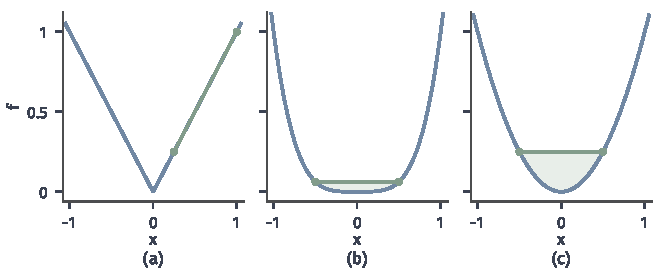
\includegraphics[width=112mm]{figures/05-optimization/01-linear-programming/matplotlib/opt-convexity-gap/figure.pdf}
  \caption{三种弯曲程度下的弦间隔，绿色线段是弦，浅绿区域是间隔。(a)$\lvert x\rvert$在同侧取端点时弦贴着图像，凸但不严格凸。(b)$x^4$严格凸，端点$\pm0.5$的中点处间隔只有$0.0625$。(c)$x^2$是$2$强凸的，同样端点的中点处间隔为$0.25$。}
  \label{fig:opt-convexity-gap}
\end{BookInlineFigure}

\paragraph{目标差控制到解的距离}
强凸性最直接的用途，是把目标值的误差换成位置的误差。

\begin{theorem}[强凸目标的二次增长]
\label{thm:opt-quadratic-growth}
设$\bm{C}$为凸集，$f$在$\bm{C}$上$\mu$强凸，且最优解$\bm{x}^\star$存在。则最优解唯一，并且对所有$\bm{x}\in\bm{C}$，
\begin{equation}
 f(\bm{x})-f^\star\geq\frac{\mu}{2}\lVert\bm{x}-\bm{x}^\star\rVert_2^2.
 \label{eq:opt-quadratic-growth}
\end{equation}
\end{theorem}

\begin{proof}
对$t\in(0,1)$，点$\bm{x}^\star+t(\bm{x}-\bm{x}^\star)$在$\bm{C}$中，目标值不低于$f^\star$。在式~\eqref{eq:opt-strong-convexity}中取$\bm{u}=\bm{x}$，$\bm{v}=\bm{x}^\star$，$\theta=t$，得到
\[
 f^\star\leq tf(\bm{x})+(1-t)f^\star-\frac{\mu}{2}t(1-t)\lVert\bm{x}-\bm{x}^\star\rVert_2^2.
\]

移项后除以$t>0$，得到
\[
 f(\bm{x})-f^\star\geq\frac{\mu}{2}(1-t)\lVert\bm{x}-\bm{x}^\star\rVert_2^2.
\]
令$t\downarrow0$即得式~\eqref{eq:opt-quadratic-growth}。若$\bm{x}$也是最优解，左端为零，迫使$\bm{x}=\bm{x}^\star$。
\end{proof}

证明只用到可行集凸、目标强凸和最优解存在，没有假设解在内部或目标可微。把实例取$\gamma=1$，由式~\eqref{eq:opt-ridge-solution}，$\bm{x}^\star=(2/3,2/3)$，$\mu=1$。取$\bm{x}=\bm{x}^\star+(1,-1)$，两个分量之和不变，所以拟合项不变，目标差全部来自正则项：
\[
 f(\bm{x})-f^\star=\frac12\bigl(\lVert\bm{x}\rVert_2^2-\lVert\bm{x}^\star\rVert_2^2\bigr)=\frac12\cdot2=1.
\]
距离的平方是$2$，式~\eqref{eq:opt-quadratic-growth}的右端也是$1$，在这里取等号，因为位移恰好沿最小特征值的方向。

可行集必须是凸的。$x^2$在$\mathbb{R}$上$2$强凸，但在$C=\{x:\lvert x\rvert\geq1\}$上有两个最小点$\pm1$，两点的目标差为$0$，距离却是$2$。证明中从$\bm{x}^\star$走向$\bm{x}$的线段离开了可行集，那一步就失效了。

表~\ref{tab:opt-convexity-ladder}汇总本节的三级要求及各自多给出的结论。

\begin{BookInlineTable}
  \centering
  \begin{tabular}{@{}lll@{}}
    \toprule
    目标（可行集凸） & 弦下方的间隔 & 结论\\
    \midrule
    凸 & 不小于$0$ & 局部最优即全局最优，解集凸\\
    严格凸 & 大于$0$ & 解至多一个\\
    $\mu$强凸 & 不小于二次量 & 解若存在则唯一，目标差控制距离\\
    \bottomrule
  \end{tabular}
  \caption{沿线段比较的三级要求。每一级都比上一级强，存在性仍需另外保证。}
  \label{tab:opt-convexity-ladder}
\end{BookInlineTable}

\section{最优解的判别}
\label{sec:opt-optimality}

前面的条件都是整体性的：可行集是否紧、目标是否凸。实际计算时，我们手里只有一个候选点，以及它附近的函数值和导数。接下来要弄清：只看这一点的导数信息，能断定什么？不能断定什么？主线讨论无约束的光滑目标，或者可行集内部的点；最后说明受约束时情况怎样改变。

全卷用$\nabla f(\bm{x})$表示梯度，$\nabla^2f(\bm{x})$表示Hessian矩阵。多元函数的梯度、Hessian和Taylor公式，可参考\BookChapterRef{chap:multivariate-differentiation}{卷二第20章“多元函数微分”}。

\paragraph{沿每个方向看}
站在最低点上，朝任何方向迈一小步都不会更低。把这句话变成计算：固定点$\bar{\bm{x}}$和方向$\bm{d}$，只看沿这条直线的一元函数
\[
 \phi(t)=f(\bar{\bm{x}}+t\bm{d}).
\]
链式法则给出它在$t=0$处的导数，即沿$\bm{d}$的\term{方向导数}（directional derivative）：
\begin{equation}
 \phi'(0)=\langle\nabla f(\bar{\bm{x}}),\bm{d}\rangle.
 \label{eq:opt-directional-derivative}
\end{equation}

$\phi'(0)<0$时，沿$\bm{d}$走一小步目标下降，这样的$\bm{d}$称为\term{下降方向}（descent direction）。条件$\langle\nabla f(\bar{\bm{x}}),\bm{d}\rangle<0$说明，只要梯度不为零，下降方向就占据整整半个空间，分界面与梯度垂直，也就是等高线在该点的切线。

用实例~\eqref{eq:opt-ridge-instance}取$\gamma=0.5$算一次。梯度的两个分量是
\[
 \frac{\partial f}{\partial x_1}=x_1+x_2-2+\gamma x_1,\qquad
 \frac{\partial f}{\partial x_2}=x_1+x_2-2+\gamma x_2.
\]
在$\bar{\bm{x}}=(2,0)$处，$\nabla f(\bar{\bm{x}})=(1,0)$。取$\bm{d}=(-1,1)$，由式~\eqref{eq:opt-directional-derivative}，方向导数是$-1$。

直接验证一下。沿这个方向$x_1+x_2$保持为$2$，拟合项为零，于是
\[
 \phi(t)=\frac14\bigl((2-t)^2+t^2\bigr),\qquad\phi'(0)=\frac14\cdot(-4)=-1.
\]
两种算法结果相同。图~\ref{fig:opt-descent-halfplane}中，浅绿半平面是全部下降方向，竖直虚线是等高线在$\bar{\bm{x}}$处的切线。负梯度方向$-\nabla f$是其中的一个，$\bm{d}$是另一个，后者比负梯度更接近指向红色最优解的方向。

\begin{BookInlineFigure}
  \centering
  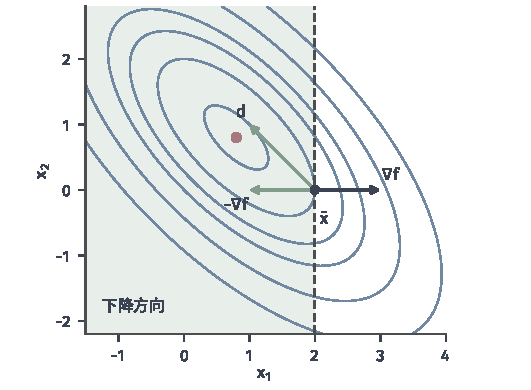
\includegraphics[width=90mm]{figures/05-optimization/01-linear-programming/matplotlib/opt-descent-halfplane/figure.pdf}
  \caption{下降方向构成半平面。蓝线是$f(\bm{x})=\frac12(x_1+x_2-2)^2+\frac14\lVert\bm{x}\rVert_2^2$的等高线，$\bar{\bm{x}}=(2,0)$处的梯度为$(1,0)$。竖直虚线与梯度垂直，浅绿区域的方向都满足$\langle\nabla f(\bar{\bm{x}}),\bm{d}\rangle<0$。绿色箭头是负梯度方向和$\bm{d}=(-1,1)$，红点是最优解$(0.8,0.8)$。}
  \label{fig:opt-descent-halfplane}
\end{BookInlineFigure}

\paragraph{一阶必要条件}
若$\bar{\bm{x}}$是局部最优解，并且各个方向都可以走，就不能有下降方向。半个空间都是下降方向的唯一例外是梯度为零。为了让“各个方向都可以走”成立，下面要求点在可行集内部：称$\bar{\bm{x}}$是$\bm{C}$的\term{内点}（interior point），如果存在$r>0$使$\bm{B}(\bar{\bm{x}},r)\subseteq\bm{C}$。

\begin{theorem}[一阶必要条件]
\label{thm:opt-first-order}
设$\bm{x}^\star$是$\bm{C}$的内点，$f$在$\bm{x}^\star$处可微。若$\bm{x}^\star$是$f$在$\bm{C}$上的局部最优解，则
\begin{equation}
 \nabla f(\bm{x}^\star)=\bm{0}.
 \label{eq:opt-first-order}
\end{equation}
\end{theorem}

\begin{proof}
任取方向$\bm{d}$。$\lvert t\rvert$充分小时，$\bm{x}^\star+t\bm{d}$既在$\bm{C}$内，又在局部最优的邻域内，所以$\phi(t)=f(\bm{x}^\star+t\bm{d})\geq\phi(0)$。

当$t>0$时，$(\phi(t)-\phi(0))/t\geq0$。令$t\downarrow0$，由式~\eqref{eq:opt-directional-derivative}得到
\[
 \langle\nabla f(\bm{x}^\star),\bm{d}\rangle\geq0.
\]
这对任意方向成立。取$\bm{d}=-\nabla f(\bm{x}^\star)$，得到$-\lVert\nabla f(\bm{x}^\star)\rVert_2^2\geq0$，所以梯度为零。
\end{proof}

梯度为零的点称为\term{驻点}（stationary point）。这个条件只是必要的，它在三处不能往下推。第一，驻点不一定是最小点：$x_1^2-x_2^2$在原点有驻点，沿$x_1$轴是最低点，沿$x_2$轴是最高点，这样的驻点称为\term{鞍点}（saddle point）。第二，定理只管内点：例子~\ref{ex:opt-local-global}的全局最优解$x=1.5$在边界上，导数不为零。第三，即使驻点是局部最优，也可能不是全局最优。

下面的二维例子同时展示这几点，后面会反复用到。考虑$\mathbb{R}^2$上的
\begin{equation}
 f(\bm{x})=x_1^3-3x_1+x_2^2.
 \label{eq:opt-cubic}
\end{equation}
令梯度为零：
\[
 \nabla f(\bm{x})=(3x_1^2-3,\ 2x_2)=\bm{0}.
\]
解得两个驻点$(1,0)$和$(-1,0)$。一阶信息到此为止，分不出这两个点的差别。

\paragraph{凸目标的驻点}
凸性能把必要条件变成充分条件。关键在于：凸函数的图像不仅在弦下方，还在每一点切线的上方。切线只用到一个点的函数值和梯度，它若是全局下界，单点信息就能告诉我们远处的目标至少有多大。

\begin{theorem}[一阶支撑不等式]
\label{thm:opt-support}
设$\bm{D}\subseteq\mathbb{R}^n$是开凸集，$f:\bm{D}\to\mathbb{R}$可微。$f$是凸函数，当且仅当对任意$\bm{u},\bm{v}\in\bm{D}$，
\begin{equation}
 f(\bm{v})\geq f(\bm{u})+\langle\nabla f(\bm{u}),\bm{v}-\bm{u}\rangle.
 \label{eq:opt-support}
\end{equation}
\end{theorem}

\begin{proof}
设$f$凸。对$t\in(0,1]$，由式~\eqref{eq:opt-convex-function}，
\[
 f\bigl(\bm{u}+t(\bm{v}-\bm{u})\bigr)\leq(1-t)f(\bm{u})+tf(\bm{v}).
\]
移项并除以$t$，得到
\[
 \frac{f\bigl(\bm{u}+t(\bm{v}-\bm{u})\bigr)-f(\bm{u})}{t}\leq f(\bm{v})-f(\bm{u}).
\]
令$t\downarrow0$，左端趋于方向导数$\langle\nabla f(\bm{u}),\bm{v}-\bm{u}\rangle$，即得式~\eqref{eq:opt-support}。

反过来，设式~\eqref{eq:opt-support}成立。取$\bm{z}=\theta\bm{u}+(1-\theta)\bm{v}$，以$\bm{z}$为切点，分别写出
\[
 f(\bm{u})\geq f(\bm{z})+\langle\nabla f(\bm{z}),\bm{u}-\bm{z}\rangle,\qquad
 f(\bm{v})\geq f(\bm{z})+\langle\nabla f(\bm{z}),\bm{v}-\bm{z}\rangle.
\]
第一式乘$\theta$，第二式乘$1-\theta$，再相加。由$\bm{z}$的定义，
\[
 \theta(\bm{u}-\bm{z})+(1-\theta)(\bm{v}-\bm{z})=\bm{0},
\]
所以内积项抵消，得到式~\eqref{eq:opt-convex-function}。
\end{proof}

图~\ref{fig:opt-support-tangent}对比了两种情形。凸函数的切线（紫色）整条位于图像下方，是全局的下界。非凸函数在$x=0$处的水平切线则位于图像上方的一大段区域，单点信息不能给出下界。

\begin{BookInlineFigure}
  \centering
  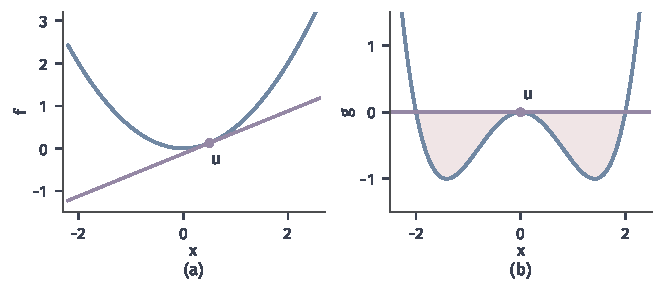
\includegraphics[width=112mm]{figures/05-optimization/01-linear-programming/matplotlib/opt-support-tangent/figure.pdf}
  \caption{切线是否是全局下界。(a)凸函数$f(x)=x^2/2$在$u=1/2$处的紫色切线整条位于图像下方。(b)非凸函数$g(x)=x^4/4-x^2$在$u=0$处的切线是水平线，在$0<\lvert x\rvert<2$时位于图像上方（浅红区域），不是下界。}
  \label{fig:opt-support-tangent}
\end{BookInlineFigure}

把$\nabla f(\bm{x}^\star)=\bm{0}$代入式~\eqref{eq:opt-support}，水平的切平面把最小值钉在切点上。

\begin{theorem}[凸目标驻点的全局最优性]
\label{thm:opt-convex-stationary}
设$\bm{D}$是开凸集，$f:\bm{D}\to\mathbb{R}$凸且可微。则$\bm{x}^\star\in\bm{D}$是$f$在$\bm{D}$上的全局最优解，当且仅当$\nabla f(\bm{x}^\star)=\bm{0}$。
\end{theorem}

\begin{proof}
必要性来自定理~\ref{thm:opt-first-order}，开集中每个点都是内点。充分性：若梯度为零，由式~\eqref{eq:opt-support}，对任意$\bm{v}\in\bm{D}$，
\[
 f(\bm{v})\geq f(\bm{x}^\star)+\langle\bm{0},\bm{v}-\bm{x}^\star\rangle=f(\bm{x}^\star).
\]
\end{proof}

这个结论的价值在于：对凸目标，求解优化问题等价于解方程$\nabla f=\bm{0}$，找到的任何一个解都是全局最优。二次拟合~\eqref{eq:opt-ridge}的梯度是
\begin{equation}
 \nabla f(\bm{x})=\bm{A}^\top(\bm{A}\bm{x}-\bm{b})+\gamma\bm{x},
 \label{eq:opt-ridge-gradient}
\end{equation}
驻点条件就是正规方程
\[
 (\bm{A}^\top\bm{A}+\gamma\bm{I})\bm{x}=\bm{A}^\top\bm{b}.
\]
实例中它化为
\[
 (1+\gamma)x_1+x_2=2,\qquad x_1+(1+\gamma)x_2=2.
\]
两式相减得$\gamma(x_1-x_2)=0$。$\gamma>0$时$x_1=x_2$，解出的正是式~\eqref{eq:opt-ridge-solution}；$\gamma=0$时两式都是$x_1+x_2=2$，解成一条直线。

强凸函数还多一个二次项。设$f$可微且$\mu$强凸。由式~\eqref{eq:opt-strong-equivalent}，$f-\frac{\mu}{2}\lVert\cdot\rVert_2^2$是凸函数，它的梯度是$\nabla f(\bm{x})-\mu\bm{x}$。对它用式~\eqref{eq:opt-support}，其中多出的项可以合并：
\[
 \lVert\bm{v}\rVert_2^2-\lVert\bm{u}\rVert_2^2-2\langle\bm{u},\bm{v}-\bm{u}\rangle=\lVert\bm{v}-\bm{u}\rVert_2^2.
\]
于是得到
\begin{equation}
 f(\bm{v})\geq f(\bm{u})+\langle\nabla f(\bm{u}),\bm{v}-\bm{u}\rangle+\frac{\mu}{2}\lVert\bm{v}-\bm{u}\rVert_2^2.
 \label{eq:opt-strong-support}
\end{equation}

这个不等式顺便补上了强凸目标的存在性。在$\mathbb{R}^n$上取$\bm{u}=\bm{0}$，由柯西不等式，
\[
 f(\bm{v})\geq f(\bm{0})-\lVert\nabla f(\bm{0})\rVert_2\lVert\bm{v}\rVert_2+\frac{\mu}{2}\lVert\bm{v}\rVert_2^2.
\]
右端在$\lVert\bm{v}\rVert_2\to\infty$时趋于$+\infty$，所以$f$强制。可微函数连续，由上一节的结论，最优解存在。再由定理~\ref{thm:opt-quadratic-growth}，最优解唯一。

\paragraph{二阶条件：曲率区分驻点的类型}
一阶条件分不清极小、极大与鞍点，因为驻点处梯度项消失了，函数的变化由下一阶主导。设$f$二阶连续可微，$\nabla f(\bm{x}^\star)=\bm{0}$。由带Lagrange余项的Taylor公式，对小的$\bm{h}$，存在$s\in(0,1)$使
\begin{equation}
 f(\bm{x}^\star+\bm{h})-f(\bm{x}^\star)=\frac12\bm{h}^\top\nabla^2f(\bm{x}^\star+s\bm{h})\bm{h}.
 \label{eq:opt-taylor}
\end{equation}
量$\bm{d}^\top\nabla^2f(\bm{x}^\star)\bm{d}$是函数沿$\bm{d}$方向的曲率：为正时向上弯，为负时向下弯。

\begin{theorem}[二阶条件]
\label{thm:opt-second-order}
设$\bm{x}^\star$是$\bm{C}$的内点，$f$在$\bm{x}^\star$附近二阶连续可微。
\begin{enumerate}
 \item 必要条件：若$\bm{x}^\star$是局部最优解，则$\nabla f(\bm{x}^\star)=\bm{0}$且$\nabla^2f(\bm{x}^\star)$半正定。
 \item 充分条件：若$\nabla f(\bm{x}^\star)=\bm{0}$且$\nabla^2f(\bm{x}^\star)$正定，则$\bm{x}^\star$是严格局部最优解。
\end{enumerate}
\end{theorem}

\begin{proof}
记$\bm{H}=\nabla^2f(\bm{x}^\star)$。先证必要条件，一阶部分即定理~\ref{thm:opt-first-order}。假设某个$\bm{d}$使$\bm{d}^\top\bm{H}\bm{d}<0$。由Hessian的连续性，$\lvert t\rvert$充分小时，对所有$s\in(0,1)$都有
\[
 \bm{d}^\top\nabla^2f(\bm{x}^\star+st\bm{d})\bm{d}<0.
\]
在式~\eqref{eq:opt-taylor}中取$\bm{h}=t\bm{d}$，就得到$f(\bm{x}^\star+t\bm{d})<f(\bm{x}^\star)$，与局部最优矛盾。

再证充分条件。记$\lambda_{\min}>0$为$\bm{H}$的最小特征值，于是
\[
 \bm{h}^\top\bm{H}\bm{h}\geq\lambda_{\min}\lVert\bm{h}\rVert_2^2.
\]
由Hessian的连续性，取足够小的$r>0$，使$\bm{B}(\bm{x}^\star,r)\subseteq\bm{C}$，并且$\lVert\bm{h}\rVert_2<r$时
\[
 \bigl\lVert\nabla^2f(\bm{x}^\star+\bm{h})-\bm{H}\bigr\rVert_2\leq\frac{\lambda_{\min}}{2}.
\]

这样对$\lVert\bm{h}\rVert_2<r$和任意$s\in(0,1)$，二次型至多比$\bm{h}^\top\bm{H}\bm{h}$小$\frac{\lambda_{\min}}{2}\lVert\bm{h}\rVert_2^2$。代入式~\eqref{eq:opt-taylor}，对$\bm{h}\neq\bm{0}$，
\[
 f(\bm{x}^\star+\bm{h})-f(\bm{x}^\star)\geq\frac12\Bigl(\lambda_{\min}-\frac{\lambda_{\min}}{2}\Bigr)\lVert\bm{h}\rVert_2^2=\frac{\lambda_{\min}}{4}\lVert\bm{h}\rVert_2^2>0.
\]
所以$\bm{x}^\star$是严格局部最优解。
\end{proof}

回到式~\eqref{eq:opt-cubic}。它的Hessian是
\[
 \nabla^2f(\bm{x})=\begin{bmatrix}6x_1&0\\0&2\end{bmatrix}.
\]
在$(1,0)$处是$\operatorname{diag}(6,2)$，正定，所以这是严格局部最优解，函数值为$-2$。在$(-1,0)$处是$\operatorname{diag}(-6,2)$，不定，不是局部最优解，也不是局部极大点，而是鞍点，函数值为$2$。

二阶条件到此仍是局部结论。沿$x_1\to-\infty$，$f\to-\infty$，所以这个问题无下界，局部最优点$(1,0)$远不是全局最优。图~\ref{fig:opt-cubic-stationary}中，穿过鞍点的粗等高线围出一个“盆”，$(1,0)$在盆底，翻过鞍点向左，地面一路下降。

\begin{BookInlineFigure}
  \centering
  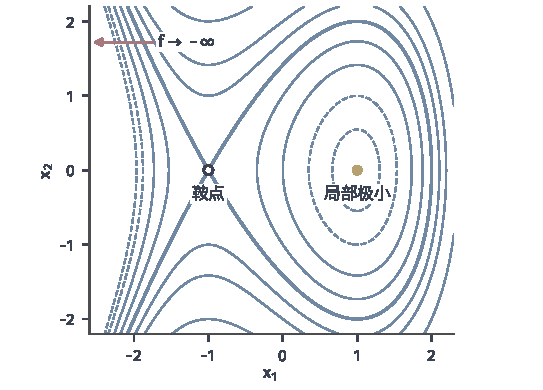
\includegraphics[width=92mm]{figures/05-optimization/01-linear-programming/matplotlib/opt-cubic-stationary/figure.pdf}
  \caption{$f(\bm{x})=x_1^3-3x_1+x_2^2$的等高线，虚线是负值水平。黄点$(1,0)$是严格局部最优解，空心点$(-1,0)$是鞍点，粗线是穿过鞍点的等高线$f=2$。红色箭头所指的左侧目标趋于$-\infty$，所以局部最优解不是全局最优解。}
  \label{fig:opt-cubic-stationary}
\end{BookInlineFigure}

要从局部曲率得到整体结论，就得要求曲率处处非负，这正是凸性的二阶判据。

\begin{theorem}[凸性的二阶判据]
\label{thm:opt-hessian-convex}
设$\bm{D}\subseteq\mathbb{R}^n$是开凸集，$f:\bm{D}\to\mathbb{R}$二阶连续可微。则$f$凸当且仅当$\nabla^2f(\bm{x})$在$\bm{D}$上处处半正定；$f$是$\mu$强凸的当且仅当$\nabla^2f(\bm{x})-\mu\bm{I}$在$\bm{D}$上处处半正定。
\end{theorem}

\begin{proof}
设$f$凸，取$\bm{x}\in\bm{D}$和方向$\bm{h}$。$t$充分小时，由式~\eqref{eq:opt-support}和带Lagrange余项的Taylor公式，存在$s\in(0,1)$使
\[
 0\leq f(\bm{x}+t\bm{h})-f(\bm{x})-t\langle\nabla f(\bm{x}),\bm{h}\rangle=\frac{t^2}{2}\bm{h}^\top\nabla^2f(\bm{x}+st\bm{h})\bm{h}.
\]
除以$t^2/2$，令$t\to0$，由Hessian的连续性得到$\bm{h}^\top\nabla^2f(\bm{x})\bm{h}\geq0$。

反过来，设Hessian处处半正定。对$\bm{u},\bm{v}\in\bm{D}$，令$\psi(t)=f(\bm{u}+t(\bm{v}-\bm{u}))$，则$\psi''\geq0$。由带Lagrange余项的Taylor公式，
\[
 \psi(1)=\psi(0)+\psi'(0)+\frac12\psi''(\xi)\geq\psi(0)+\psi'(0),
\]
这正是式~\eqref{eq:opt-support}，由定理~\ref{thm:opt-support}，$f$凸。

强凸的情形，把上述结论用于$f-\frac{\mu}{2}\lVert\cdot\rVert_2^2$，它的Hessian是$\nabla^2f-\mu\bm{I}$，再用式~\eqref{eq:opt-strong-equivalent}。
\end{proof}

判据要求在整个开凸集上成立，只在单个点检查不能证明函数凸。式~\eqref{eq:opt-cubic}在$(1,0)$处Hessian正定，但在$x_1<0$处有负特征值，所以它不是凸函数，局部最优也就不必是全局最优。二次拟合的Hessian处处等于$\bm{A}^\top\bm{A}+\gamma\bm{I}$，半正定，这与前面用弦算出的结论一致。

\paragraph{退化驻点：二阶也判不了}
定理~\ref{thm:opt-second-order}的两个条件之间留有缺口：Hessian半正定但奇异时，必要条件满足，充分条件不满足，二阶信息不足以判断。这样的驻点称为\term{退化驻点}（degenerate stationary point）。

函数$x_1^2+x_2^4$和$x_1^2+x_2^3$在原点的梯度都为零，Hessian都是$\operatorname{diag}(2,0)$，二阶信息完全相同。前者对$\bm{x}\neq\bm{0}$恒为正，原点是严格最小点，说明正定不是必要的。后者沿$(0,-t)$取值$-t^3<0$，原点不是局部最优解，说明半正定不是充分的。

决定结果的是$x_2$方向的高阶项，这正是Hessian在零特征方向上看不到的信息。图~\ref{fig:opt-stationary-types}中，请注意红色区域是否碰到原点：碰到就说明任意小的邻域里都有更低的点。(c)与(d)的二阶信息相同，红色区域却一有一无。

\begin{BookInlineFigure}
  \centering
  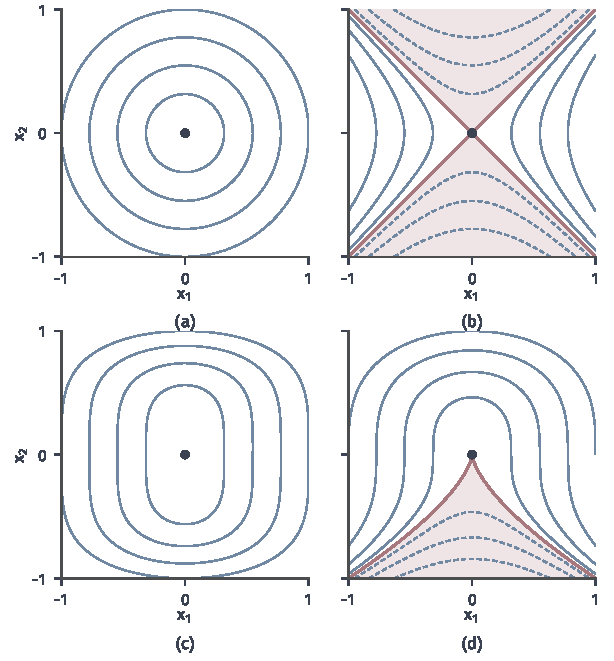
\includegraphics[width=104mm]{figures/05-optimization/01-linear-programming/matplotlib/opt-stationary-types/figure.pdf}
  \caption{原点处四种驻点的等高线，浅红区域是函数值低于$f(\bm{0})=0$的点，虚线是负值水平，红线是零等高线。(a)$x_1^2+x_2^2$，Hessian正定，严格最小点。(b)$x_1^2-x_2^2$，Hessian不定，鞍点。(c)$x_1^2+x_2^4$，Hessian为$\operatorname{diag}(2,0)$，仍是严格最小点。(d)$x_1^2+x_2^3$，Hessian同为$\operatorname{diag}(2,0)$，但原点下方有更低的点，不是局部最优解。}
  \label{fig:opt-stationary-types}
\end{BookInlineFigure}

\paragraph{负曲率方向}
定理~\ref{thm:opt-second-order}必要性的证明还包含一条可以操作的信息。若驻点处存在方向$\bm{d}$使$\bm{d}^\top\nabla^2f(\bm{x}^\star)\bm{d}<0$，就称$\bm{d}$为\term{负曲率方向}（negative curvature direction）。沿它走，一阶变化为零，目标却以二次速度下降。

对$f(\bm{x})=x_1^2-x_2^2$，Hessian是$\operatorname{diag}(2,-2)$。沿单位方向$\bm{d}$，
\[
 f(t\bm{d})=\frac{t^2}{2}\bm{d}^\top\operatorname{diag}(2,-2)\bm{d}=t^2(d_1^2-d_2^2).
\]
图~\ref{fig:opt-saddle-curvature}取三个方向：$\bm{d}_1=(1,0)$曲率为$2$，向上弯；$\bm{d}_2=(1,1)/\sqrt2$曲率为$0$，二阶项恰好消失；$\bm{d}_3=(0,1)$曲率为$-2$，向下弯。站在鞍点上，梯度指不出任何下降方向，Hessian的负特征向量却指出了一条。怎样利用这一点离开鞍点，由第~\ref{chap:saddle-points}章讨论。

\begin{BookInlineFigure}
  \centering
  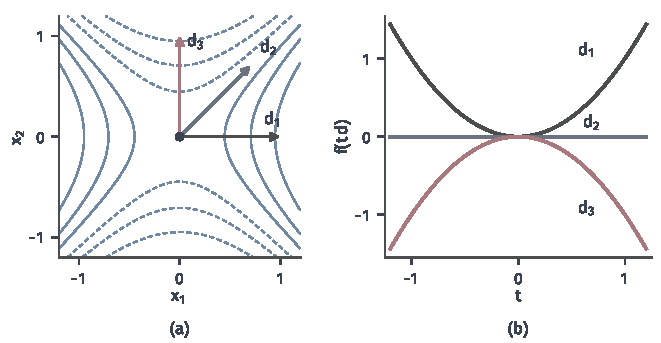
\includegraphics[width=112mm]{figures/05-optimization/01-linear-programming/matplotlib/opt-saddle-curvature/figure.pdf}
  \caption{鞍点处不同方向的曲率。(a)$f(\bm{x})=x_1^2-x_2^2$的等高线（虚线为负值）与三个单位方向。(b)沿这三个方向的一元限制$f(t\bm{d})$：$\bm{d}_1$向上弯，$\bm{d}_2$保持为零，红色的$\bm{d}_3$向下弯，是负曲率方向。}
  \label{fig:opt-saddle-curvature}
\end{BookInlineFigure}

表~\ref{tab:opt-tests}整理到目前为止的判别依据。阅读时要注意“必要”与“充分”的方向，以及结论是局部的还是全局的。

\begin{BookInlineTable}
  \centering
  \begin{tabular}{@{}lll@{}}
    \toprule
    依据 & 性质 & 能得到的结论\\
    \midrule
    $\nabla f=\bm{0}$ & 内点局部最优的必要条件 & 排除非驻点\\
    $\nabla f=\bm{0}$，$\nabla^2f\succeq\bm{0}$ & 局部最优的必要条件 & 进一步排除负曲率点\\
    $\nabla f=\bm{0}$，$\nabla^2f\succ\bm{0}$ & 充分条件，非必要 & 严格局部最优\\
    $\nabla f=\bm{0}$，目标凸 & 充要条件 & 全局最优\\
    \bottomrule
  \end{tabular}
  \caption{无约束光滑目标的判别依据。前三行只看一个点，第四行需要目标的整体性质。}
  \label{tab:opt-tests}
\end{BookInlineTable}

\paragraph{受约束时允许的方向变了}
一阶条件的证明要求$\bm{d}$和$-\bm{d}$都能走。在边界上这个前提不成立，能走的方向变少，要求也相应放宽。称$\bm{d}$是$\bar{\bm{x}}\in\bm{C}$处的\term{可行方向}（feasible direction），如果$t>0$充分小时$\bar{\bm{x}}+t\bm{d}\in\bm{C}$。重复定理~\ref{thm:opt-first-order}证明的前半段，只用$t>0$，就得到：若$\bm{x}^\star$是局部最优解，$f$在该点可微，则对每个可行方向$\bm{d}$，
\begin{equation}
 \langle\nabla f(\bm{x}^\star),\bm{d}\rangle\geq0.
 \label{eq:opt-feasible-direction}
\end{equation}

用资源分配验证。在$\bm{x}^\star=(2,2)$处，两条资源约束取等号，$\bm{d}$可行当且仅当它不增加这两个约束，即
\[
 d_1+d_2\leq0,\qquad 2d_1+d_2\leq0.
\]
目标的梯度是$(-3,-2)$，不等于零。方向导数却可以拆开：
\[
 \langle\nabla f(\bm{x}^\star),\bm{d}\rangle=-3d_1-2d_2=-(d_1+d_2)-(2d_1+d_2)\geq0.
\]

这里的拆分仍然是第~\ref{sec:opt-formulation}节那个“两条约束相加”。图~\ref{fig:opt-boundary-directions}显示了几何含义：$-\nabla f$指向利润增大的方向，它伸出了可行集，而所有绿色的可行方向都和它成钝角或直角。所以$(2,2)$处梯度不为零，却没有“既可行又下降”的方向。

\begin{BookInlineFigure}
  \centering
  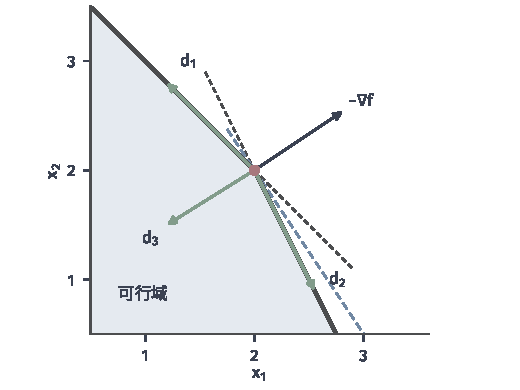
\includegraphics[width=88mm]{figures/05-optimization/01-linear-programming/matplotlib/opt-boundary-directions/figure.pdf}
  \caption{边界上的最优点梯度不必为零。红点是资源分配的最优解$(2,2)$，深灰粗线是两条取等号的约束，蓝色虚线是过该点的等目标线。绿色箭头是可行方向，全部可行方向都夹在$\bm{d}_1=(-1,1)$与$\bm{d}_2=(1,-2)$之间。$-\nabla f=(3,2)$伸出可行集，与每个可行方向的内积都不为正。}
  \label{fig:opt-boundary-directions}
\end{BookInlineFigure}

若$\bm{C}$凸、$f$在包含$\bm{C}$的开凸集上凸且可微，式~\eqref{eq:opt-feasible-direction}对每个$\bm{d}=\bm{y}-\bm{x}^\star$（$\bm{y}\in\bm{C}$）成立时，代入式~\eqref{eq:opt-support}就得到$f(\bm{y})\geq f(\bm{x}^\star)$，所以它也是充分的。

式~\eqref{eq:opt-feasible-direction}还不是一个能直接检验的判据。可行方向可能有无穷多个，曲线边界上甚至可能一个非零的都没有：单位圆周上，沿任何直线都会立刻离开圆周。把它写成关于约束函数的代数条件需要新工具，第~\ref{chap:constrained-optimality}章在明确约束之后建立这些判别。

\section{近似解的评价}
\label{sec:opt-approximate}

前四节讨论的是精确的解。实际计算几乎从不交出精确解：迭代在有限步后停止，浮点运算带来舍入。这就需要回答：拿到一个近似解，怎样说清它好到什么程度？我们会看到，“好”有几种不同的含义，它们回答不同的问题，只在一定条件下可以换算。

\paragraph{算法交出什么}
后面各章的方法都产生一列点。全卷用带括号的上标表示迭代步：$\bm{x}^{(t)}$是第$t$步的点，$t=0,1,\ldots,T$，$T$是总步数。括号把迭代编号与幂区分开，元素下标仍写在下面，如$x_i^{(t)}$。多数方法每一步沿某个方向走一段：
\begin{equation}
 \bm{x}^{(t+1)}=\bm{x}^{(t)}+\alpha^{(t)}\bm{d}^{(t)},
 \label{eq:opt-iteration}
\end{equation}
其中$\bm{d}^{(t)}$是方向，$\alpha^{(t)}>0$是步长。当前点的梯度和Hessian简记为$\bm{g}^{(t)}=\nabla f(\bm{x}^{(t)})$与$\bm{H}^{(t)}=\nabla^2f(\bm{x}^{(t)})$。

算法最后报告的点记为$\hat{\bm{x}}$。本节不关心它怎样得到，只关心怎样评价。要注意$\hat{\bm{x}}$与$\bm{x}^\star$的区别：前者是算法的输出，手里实实在在有；后者是问题的解，我们通常不知道。

\paragraph{目标差}
最直接的指标是目标差
\begin{equation}
 e_f(\hat{\bm{x}})=f(\hat{\bm{x}})-f^\star.
 \label{eq:opt-objective-gap}
\end{equation}
它回答“这个结果比最好的结果差多少”。可行点的目标差非负；若$\hat{\bm{x}}$可行且$e_f(\hat{\bm{x}})\leq\varepsilon$，就称它为$\varepsilon$最优解（$\varepsilon$-optimal solution）。

目标差的麻烦在于$f^\star$通常未知。但只要有一个下界$\ell\leq f^\star$，就有可以计算的上界$e_f(\hat{\bm{x}})\leq f(\hat{\bm{x}})-\ell$。资源分配中，“两条约束相加”给出了下界$\ell=-10$，它不依赖于解出$(2,2)$。对可行点$\hat{\bm{x}}=(1.5,2)$，利润是$8.5$，因此
\[
 f(\hat{\bm{x}})-\ell=-8.5-(-10)=1.5.
\]
这正是上下界夹逼的用处：不知道解在哪里，也能确认当前结果至多差$1.5$。这样的下界怎样系统地构造，是第~\ref{chap:duality}章的主题。

\paragraph{解距离}
第二个指标问位置差多远。设最优解集合$\bm{S}$非空，定义到解集的距离
\begin{equation}
 e_d(\hat{\bm{x}})=\operatorname{dist}(\hat{\bm{x}},\bm{S})=\inf_{\bm{x}\in\bm{S}}\lVert\hat{\bm{x}}-\bm{x}\rVert_2.
 \label{eq:opt-solution-distance}
\end{equation}
解唯一时，它就是$\lVert\hat{\bm{x}}-\bm{x}^\star\rVert_2$。

解不唯一时要注意参照对象。实例~\eqref{eq:opt-ridge-instance}取$\gamma=0$，点$(11,-9)$在直线$x_1+x_2=2$上，它本身就是最优解，到解集的距离为$0$。若心里的“正确系数”是$(1,1)$，两者却相距$\lVert(10,-10)\rVert_2\approx14.1$。把解距离写成到某一个解的距离，就在问题没有提供信息的地方提了要求。

\paragraph{梯度大小}
前两个指标都含有未知量，第三个可以直接算：
\begin{equation}
 e_g(\hat{\bm{x}})=\lVert\nabla f(\hat{\bm{x}})\rVert_2.
 \label{eq:opt-gradient-size}
\end{equation}
由第~\ref{sec:opt-optimality}节，无约束时局部最优解的梯度为零，所以梯度大小可以作为一种缺口的度量。满足$e_g(\hat{\bm{x}})\leq\varepsilon$的点称为$\varepsilon$驻点（$\varepsilon$-stationary point）。

梯度小却不等于接近解。图~\ref{fig:opt-flat-gradient}(a)比较$f_1(x)=0.005x^2$与$f_2(x)=0.5x^2$，两者的最小点都是$0$。在$x=10$处$f_1'=0.1$，在$x=0.1$处$f_2'=0.1$，梯度一样大。前者的目标差是$0.5$，距离是$10$；后者分别是$0.005$和$0.1$。原因在曲率：$f_1$的二阶导数只有$0.01$，地形太平，坡度很小时离谷底仍然很远。

\begin{BookInlineFigure}
  \centering
  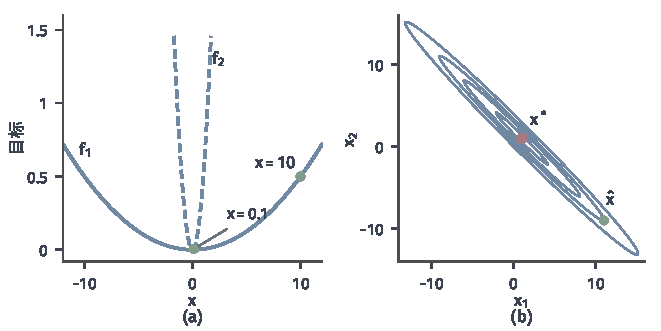
\includegraphics[width=112mm]{figures/05-optimization/01-linear-programming/matplotlib/opt-flat-gradient/figure.pdf}
  \caption{小梯度与小误差。(a)平坦的$f_1(x)=0.005x^2$（实线）在$x=10$处与陡峭的$f_2(x)=0.5x^2$（虚线）在$x=0.1$处导数都是$0.1$，目标差和距离却相差约两个量级。(b)拟合实例取$\gamma=0.01$，蓝线是目标差等于$0.1,0.5,1,2$的等高线，沿$(1,-1)$方向被拉得极长。绿点$\hat{\bm{x}}=(11,-9)$的梯度大小约为$0.142$，到红点$\bm{x}^\star$的距离约为$14.1$。}
  \label{fig:opt-flat-gradient}
\end{BookInlineFigure}

二维的情形更说明问题。实例~\eqref{eq:opt-ridge-instance}取$\gamma=0.01$，由式~\eqref{eq:opt-ridge-solution}，解和最优值是
\[
 \bm{x}^\star\approx(0.995,0.995),\qquad f^\star\approx0.00995.
\]
取$\hat{\bm{x}}=(11,-9)$。两分量之和为$2$，拟合项为零，于是目标值和梯度分别是
\[
 f(\hat{\bm{x}})=0.005\cdot(121+81)=1.01,\qquad\nabla f(\hat{\bm{x}})=(0.11,-0.09).
\]

三个指标的数值是
\[
 e_f\approx1.000,\qquad e_d\approx14.14,\qquad e_g\approx0.142.
\]
观测已经完美拟合，梯度也不大，点却在长沟里离解很远。图~\ref{fig:opt-flat-gradient}(b)的长沟就是强凸常数$\mu=0.01$很小的样子。

驻点还有另一重不足：非凸目标的驻点可以根本不是局部最优解。式~\eqref{eq:opt-cubic}的鞍点$(-1,0)$梯度为零，$e_g=0$，而这个问题甚至没有下界。所以“算法找到驻点”和“算法找到解”是两个强度不同的结论。

\paragraph{三种指标的容差集合}
把三个指标都限定在同一个$\varepsilon$以内，得到三个不同形状的区域。以二次目标为例，记位移$\bm{w}=\bm{x}-\bm{x}^\star$。由$\nabla f(\bm{x}^\star)=\bm{0}$，三个区域分别是
\[
 \tfrac12\bm{w}^\top\bm{H}\bm{w}\leq\varepsilon,\qquad
 \lVert\bm{w}\rVert_2\leq\varepsilon,\qquad
 \lVert\bm{H}\bm{w}\rVert_2\leq\varepsilon.
\]
图~\ref{fig:opt-tolerance-regions}取实例$\gamma=0.1$，$\varepsilon=0.1$。圆很小；目标差的椭圆沿平坦方向半轴为$\sqrt{2\varepsilon/\gamma}\approx1.41$；梯度的椭圆沿平坦方向半轴为$\varepsilon/\gamma=1$，沿陡峭方向只有$\varepsilon/(2+\gamma)\approx0.048$。

三个区域互不包含，所以“达到精度$\varepsilon$”必须说明用的是哪个指标。沿平坦方向，目标差和梯度都很宽容；沿陡峭方向，梯度最严格。

\begin{BookInlineFigure}
  \centering
  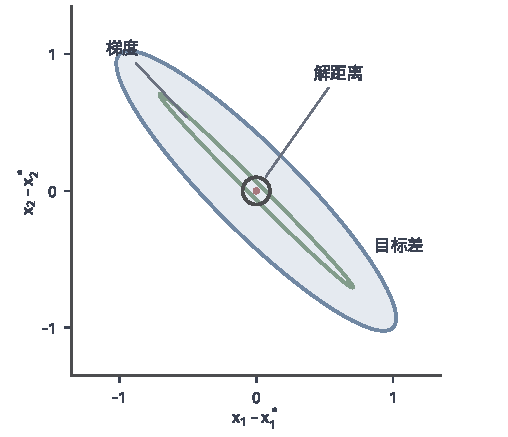
\includegraphics[width=86mm]{figures/05-optimization/01-linear-programming/matplotlib/opt-tolerance-regions/figure.pdf}
  \caption{同一个$\varepsilon=0.1$下三种指标的容差集合，横纵轴是相对于$\bm{x}^\star$的位移，目标取$\gamma=0.1$的拟合实例，$\bm{H}$的特征值为$0.1$和$2.1$。蓝色椭圆内目标差不超过$\varepsilon$，绿色椭圆内梯度大小不超过$\varepsilon$，深灰色小圆内解距离不超过$\varepsilon$。}
  \label{fig:opt-tolerance-regions}
\end{BookInlineFigure}

\paragraph{换算的条件：曲率的上下界}
前面的例子都指向曲率。把它变成定量结论，需要两个常数：曲率的下界$\mu$和上界$L$。全卷用$L$表示光滑常数，用$\kappa=L/\mu$表示条件数。这里先在二阶可微的情形下引入，用$\bm{A}\preceq\bm{B}$表示$\bm{B}-\bm{A}$半正定。第~\ref{chap:smooth-foundations}章将把$L$推广到只要求梯度Lipschitz连续的函数。

\begin{theorem}[三种误差的换算]
\label{thm:opt-error-conversions}
设$f:\mathbb{R}^n\to\mathbb{R}$二阶连续可微，且存在$0<\mu\leq L$，使对所有$\bm{x}$，
\begin{equation}
 \mu\bm{I}\preceq\nabla^2f(\bm{x})\preceq L\bm{I}.
 \label{eq:opt-curvature-bounds}
\end{equation}
则$f$有唯一最优解$\bm{x}^\star$，并且对任意$\bm{x}$，
\begin{equation}
 \begin{gathered}
 \frac{\mu}{2}e_d^2\leq e_f\leq\frac{L}{2}e_d^2,\qquad
 \mu e_d\leq e_g\leq Le_d,\\
 \frac{1}{2L}e_g^2\leq e_f\leq\frac{1}{2\mu}e_g^2.
 \end{gathered}
 \label{eq:opt-error-conversions}
\end{equation}
\end{theorem}

\begin{proof}
由定理~\ref{thm:opt-hessian-convex}，$f$是$\mu$强凸的，由第~\ref{sec:opt-optimality}节的结论，最优解存在且唯一。记$\bm{w}=\bm{x}-\bm{x}^\star$，$e_d=\lVert\bm{w}\rVert_2$。

第一组：由式~\eqref{eq:opt-taylor}，存在$s\in(0,1)$使
\[
 e_f=\frac12\bm{w}^\top\nabla^2f(\bm{x}^\star+s\bm{w})\bm{w}.
\]
再用式~\eqref{eq:opt-curvature-bounds}夹住二次型，即得。

第二组：由$\nabla f(\bm{x}^\star)=\bm{0}$和微积分基本定理，
\[
 \nabla f(\bm{x})=\bm{B}\bm{w},\qquad\bm{B}=\int_0^1\nabla^2f(\bm{x}^\star+s\bm{w})\,\mathrm{d}s.
\]
$\bm{B}$对称，其二次型是被积函数二次型的积分，所以特征值都在$[\mu,L]$内，于是
\[
 \mu\lVert\bm{w}\rVert_2\leq\lVert\bm{B}\bm{w}\rVert_2\leq L\lVert\bm{w}\rVert_2.
\]

第三组的右半：在式~\eqref{eq:opt-strong-support}中取$\bm{u}=\bm{x}$，右端是$\bm{v}$的二次函数，在$\bm{v}=\bm{x}-\nabla f(\bm{x})/\mu$处最小。所以对所有$\bm{v}$，
\[
 f(\bm{v})\geq f(\bm{x})-\frac{1}{2\mu}\lVert\nabla f(\bm{x})\rVert_2^2.
\]
取$\bm{v}=\bm{x}^\star$即得$e_f\leq e_g^2/(2\mu)$。

第三组的左半：由Taylor公式和$\nabla^2f\preceq L\bm{I}$，对任意$\bm{p}$有
\[
 f(\bm{x}+\bm{p})\leq f(\bm{x})+\langle\nabla f(\bm{x}),\bm{p}\rangle+\frac{L}{2}\lVert\bm{p}\rVert_2^2.
\]
取$\bm{p}=-\nabla f(\bm{x})/L$，得到
\[
 f^\star\leq f\Bigl(\bm{x}-\frac{1}{L}\nabla f(\bm{x})\Bigr)\leq f(\bm{x})-\frac{1}{2L}\lVert\nabla f(\bm{x})\rVert_2^2.
\]
移项即得$e_f\geq e_g^2/(2L)$。
\end{proof}

图~\ref{fig:opt-metric-conversions}把式~\eqref{eq:opt-error-conversions}画成一张换算图，每条箭头表示“已知箭尾的量，可以控制箭头的量”。凡用到$\mu$的箭头，都是从目标值或梯度推断位置，需要下弯曲率；用到$L$的箭头，是从位置推断目标值或梯度，需要上弯曲率有限。

\begin{BookInlineFigure}
  \centering
  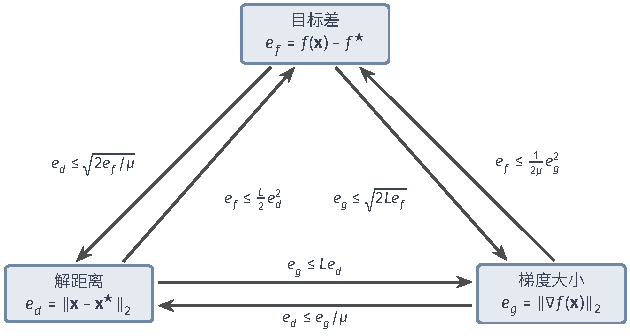
\includegraphics[width=106.74mm]{figures/05-optimization/01-linear-programming/tikz/opt-metric-conversions/figure.pdf}
  \caption{无约束时三种误差的换算，条件是$\mu\bm{I}\preceq\nabla^2f\preceq L\bm{I}$。箭头从已知量指向被控制的量。可计算的只有右下角的梯度大小，它指向其余两个量的两条箭头都依赖$\mu$。}
  \label{fig:opt-metric-conversions}
\end{BookInlineFigure}

用$\gamma=0.01$的实例代入。此时$\mu=0.01$，$L=2.01$，$\kappa=201$。对$\hat{\bm{x}}=(11,-9)$，右半边的两个上界是
\[
 e_f\leq\frac{e_g^2}{2\mu}\approx\frac{0.0202}{0.02}=1.01,\qquad
 e_d\leq\frac{e_g}{\mu}\approx14.2.
\]
实际值是$1.000$和$14.14$，两个界都很贴近，因为$\hat{\bm{x}}-\bm{x}^\star$几乎沿着平坦方向。而梯度约$0.142$这个数看起来很小，放大$1/\mu=100$倍后才是真实的距离。

两个常数不能互相替代，缺了一个，相应的箭头就断了。$\mu$接近零时，梯度几乎不提供关于目标差和距离的信息。$L$不存在时，距离小也不能保证梯度小：$\lvert x\rvert$在任意靠近$0$的点$x\neq0$处，梯度大小都是$1$。$\kappa$大表示两个方向的曲率差得远，同一个$e_d$对应的$e_g$可以相差$\kappa$倍。

\paragraph{有约束时：可行性}
定理~\ref{thm:opt-error-conversions}只针对无约束问题。有约束时，算法的输出可能不满足约束，目标差本身也就失去了意义。用\term{可行性残差}（feasibility residual）度量违反的程度：
\begin{equation}
 r_{\mathrm{feas}}(\hat{\bm{x}})=\max\Bigl\{\max_{i}\,\max\{g_i(\hat{\bm{x}}),0\},\ \max_{j}\,\lvert h_j(\hat{\bm{x}})\rvert\Bigr\}.
 \label{eq:opt-feasibility-residual}
\end{equation}
可行点的残差为零，残差大于零的点违反了至少一条约束。

资源分配中取点$\tilde{\bm{x}}=(2.1,2)$，它违反了两条资源约束：
\[
 g_1(\tilde{\bm{x}})=0.1,\qquad g_2(\tilde{\bm{x}})=0.2,\qquad r_{\mathrm{feas}}(\tilde{\bm{x}})=0.2.
\]
它的利润是$10.3$，比最优利润还高，也就是$f(\tilde{\bm{x}})-f^\star=-0.3<0$。多出来的利润并不是好事，它来自多用的资源。把两条约束相加的论证用在这里，利润至多超出$g_1+g_2=0.3$，恰好等于$0.3$。

反过来，可行点$(0,0)$的残差为零，利润却是$0$，目标差为$10$。图~\ref{fig:opt-feasibility-gap}中，绿点可行但利润不足，红叉利润过高但不可行。所以只报告目标值或只报告可行性都不够，两者要一起报告。

\begin{BookInlineFigure}
  \centering
  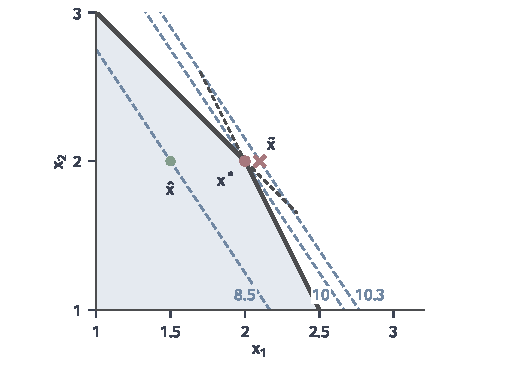
\includegraphics[width=88mm]{figures/05-optimization/01-linear-programming/matplotlib/opt-feasibility-gap/figure.pdf}
  \caption{目标值与可行性要一起看。浅蓝区域是资源分配的部分可行集，蓝色虚线旁的数字是利润。绿点$\hat{\bm{x}}=(1.5,2)$可行，利润$8.5$；红点$\bm{x}^\star=(2,2)$是最优解，利润$10$；红叉$\tilde{\bm{x}}=(2.1,2)$利润$10.3$，高于最优值，但违反了两条资源约束。}
  \label{fig:opt-feasibility-gap}
\end{BookInlineFigure}

约束的数值量纲也影响残差。把“工时”的单位换成分钟，同一条约束乘以$60$，残差也放大$60$倍，可行集却没有变。比较之前要先把约束的尺度说清楚。

\paragraph{有约束时：最优性残差}
第~\ref{sec:opt-optimality}节的图~\ref{fig:opt-boundary-directions}说明，有约束时梯度大小不再是合适的度量：最优解处的梯度不必为零。\term{最优性残差}（optimality residual）指这样一类量：在当前点可以计算，并且恰好在一阶条件成立时为零。无约束时它就是梯度大小。

一个能手算的情形是盒约束$\bm{C}=\{\bm{x}:l_i\leq x_i\leq u_i\}$，上下界允许取无穷。记$\Pi_{\bm{C}}$为逐坐标截断到$[l_i,u_i]$的投影，定义
\begin{equation}
 \bm{r}(\bm{x})=\bm{x}-\Pi_{\bm{C}}\bigl(\bm{x}-\nabla f(\bm{x})\bigr).
 \label{eq:opt-projected-residual}
\end{equation}
逐坐标看，记$g_i$为此处的第$i$个偏导数：$x_i$严格在区间内部时，$r_i=0$要求$g_i=0$；$x_i=l_i$时，$r_i=0$只要求$g_i\geq0$；$x_i=u_i$时，只要求$g_i\leq0$。这正是可行方向条件~\eqref{eq:opt-feasible-direction}逐坐标的写法。

取实例$\gamma=0.5$，加约束$x_1\geq1.2$。解在边界上：固定$x_1=1.2$，对$x_2$最小化得$x_2=8/15$，点$\bm{x}^\star=(1.2,8/15)$。此处的梯度由式~\eqref{eq:opt-ridge-gradient}算得
\[
 \nabla f(\bm{x}^\star)=\Bigl(\frac13,\ 0\Bigr).
\]
梯度不为零，但第一个坐标在下界上，偏导数非负，$\bm{r}(\bm{x}^\star)=\bm{0}$。这个问题是凸的，由上一节的充分性，$\bm{x}^\star$确实是最优解。

再看一个不是解的可行点$\hat{\bm{x}}=(1.5,0.5)$。此处$\nabla f(\hat{\bm{x}})=(0.75,0.25)$，先走一步再截断：
\[
 \hat{\bm{x}}-\nabla f(\hat{\bm{x}})=(0.75,0.25),\qquad
 \Pi_{\bm{C}}(0.75,0.25)=(1.2,0.25).
\]
所以$\bm{r}(\hat{\bm{x}})=(0.3,0.25)$，范数约为$0.39$。这个残差告诉我们，点还没有满足一阶条件。

一般约束的最优性残差要用到约束梯度的组合，由第~\ref{chap:constrained-optimality}章建立；非光滑目标没有梯度，相应的量由第~\ref{chap:nonsmooth-composite-optimization}章定义。这里只需记住它的职责：在不知道解的情况下，度量当前点离一阶条件还差多少。

\paragraph{精度标准}
表~\ref{tab:opt-metrics}汇总这些指标。后续各章陈述结果时，都要说清用的是哪一个。

\begin{table*}[!htbp]
  \centering
  \begin{tabular}{@{}llll@{}}
    \toprule
    指标 & 回答的问题 & 能否直接计算 & 换算所需条件\\
    \midrule
    目标差$e_f$ & 结果比最好差多少 & 需要$f^\star$或其下界 & 可行点；$\mu$可换成距离，$L$可换成梯度\\
    解距离$e_d$ & 位置差多远 & 需要解集 & 解不唯一时参照解集；$L$可换成目标差和梯度\\
    梯度大小$e_g$ & 局部还有多少下降余地 & 能 & 无约束；$\mu$才能换成目标差和距离\\
    可行性残差$r_{\mathrm{feas}}$ & 违反约束多少 & 能 & 依赖约束的尺度\\
    最优性残差 & 离一阶条件还差多少 & 能 & 凸问题中才对应全局最优\\
    \bottomrule
  \end{tabular}
  \caption{近似解的评价指标。前三项针对无约束或已知可行的点，后两项用于约束问题；换算条件的含义见定理~\ref{thm:opt-error-conversions}。}
  \label{tab:opt-metrics}
\end{table*}

阈值的取法也要交代。绝对标准$e_g\leq\varepsilon$依赖目标的尺度：把$f$整体乘以$100$，解不变，梯度却放大$100$倍，同一个$\varepsilon$的严格程度就变了。所以实践中常用相对标准，例如
\begin{equation}
 \lVert\bm{g}^{(t)}\rVert_2\leq\varepsilon\,\max\bigl\{1,\lVert\bm{g}^{(0)}\rVert_2\bigr\}.
 \label{eq:opt-relative-stopping}
\end{equation}

评价方法与决定停止是两种场合。比较方法时，常对同一问题先用高精度方法算出参照值$f^\star$，再看目标差随计算量的变化；参照值本身也有误差，应当说明怎样得到。实际求解时$f^\star$未知，只能依据可计算的残差决定何时停止，而残差小对目标差意味着什么，取决于$\mu$这样的条件。

最后要区分算法的结论。说“迭代收敛到驻点”“输出满足$e_g\leq\varepsilon$”“输出是$\varepsilon$最优解”，是三个强度依次上升的陈述，中间隔着凸性或曲率下界这样的条件。迭代次数与每步代价怎样计入比较，由第~\ref{chap:smooth-foundations}章规定。

\section{本章小结}
\label{sec:opt-summary}

本章把“在允许的选择里找最好的”拆成了几个分别回答的问题。写一个优化问题要同时给出决策变量、目标函数和可行集。最优值是下确界，最优解是取得它的可行点，两者可以分离：问题可能不可行、无下界，或最优值有限却未被达到。局部最优只和附近的可行点比较，全局最优和所有可行点比较。约束指标函数把约束并入目标而不改变问题，普通指示函数和有限惩罚则不能这样用。

存在性靠最小化序列的三关：留得住、极限合法、比较传得到。紧性通过前两关，下半连续通过第三关，无界可行集用紧下水平集或强制性处理。解的性质靠线段比较：凸性使局部最优成为全局最优，严格凸使解至多一个，强凸使目标差控制到解的距离。

判别依赖一个点的导数信息。一阶和二阶条件在内点上区分驻点、局部最优和鞍点，它们本身是局部的；只有目标凸时，驻点才是全局最优。边界上的最优点梯度可以不为零，因为允许的方向变少了。

两个贯穿的例子展示了这些问题怎样得到回答。资源分配的可行集是有界多面体，解存在；把两条资源约束相加，同时得到下界和达到它的点$(2,2)$。二次拟合的$\gamma>0$让目标强制，又让Hessian正定，解存在且唯一，目标差可以换成距离；$\gamma=0$且$\bm{A}$秩亏时，目标不再强制，解仍存在，却成了一条直线。

表~\ref{tab:opt-summary}汇总各结论所需的条件，表中均为充分条件，反例列说明去掉条件或反向推断时的后果。

\begin{table*}[!htbp]
\centering
\small
\begin{tabularx}{\linewidth}{@{}>{\RaggedRight\arraybackslash}p{24mm}>{\RaggedRight\arraybackslash}X>{\RaggedRight\arraybackslash}X>{\RaggedRight\arraybackslash}X@{}}
\toprule
问题 & 充分条件 & 结论 & 反例或边界 \\
\midrule
最优解是否存在 & 可行集非空紧，目标下半连续且有有限值；或某个下水平集非空紧 & 最优值有限且被达到 & $(0,1]$上的$x$；$[1,\infty)$上的$1/x$；在$0$处跳高的函数 \\
局部是否即全局 & 可行集凸，目标凸 & 局部最优解都是全局最优解，解集凸 & 例子中的四次函数；$[-3,-1]\cup[1,3]$上的$(x-2)^2$ \\
解是否唯一 & 可行集凸，目标严格凸，解存在 & 解唯一 & $e^x$严格凸而无最小点；$\lvert x\rvert$与资源分配有唯一解而不严格凸 \\
目标差能否换成距离 & 可行集凸，目标$\mu$强凸，解存在 & $f(\bm{x})-f^\star\geq\frac{\mu}{2}\lVert\bm{x}-\bm{x}^\star\rVert_2^2$ & 非凸可行集$\{\lvert x\rvert\geq1\}$上的$x^2$ \\
内点能否用梯度判别 & 可微；开凸集上目标凸 & 局部最优必有$\nabla f=\bm{0}$；凸时$\nabla f=\bm{0}$即全局最优 & 鞍点；边界最优点的导数可不为零 \\
驻点是否局部最优 & 二阶连续可微，Hessian正定 & 严格局部最优解 & $x_1^2+x_2^4$（正定非必要）；$x_1^2+x_2^3$（半正定不充分）\\
小梯度是否表示小误差 & $\mu\bm{I}\preceq\nabla^2f\preceq L\bm{I}$，无约束 & $e_f\leq e_g^2/(2\mu)$，$e_d\leq e_g/\mu$ & 平坦目标$0.005x^2$；$\gamma=0.01$的拟合实例 \\
\bottomrule
\end{tabularx}
\caption{本章主要问题、充分条件与边界。}
\label{tab:opt-summary}
\end{table*}

算法的输出和问题的解是两回事。输出$\hat{\bm{x}}$由目标差、解距离、梯度大小、可行性残差和最优性残差分别衡量，它们回答不同的问题，只有在曲率上下界这样的条件下才能换算，系数随$1/\mu$放大。

本章没有构造任何算法。从下一章起，线性规划把这些语言用在最具体的模型上：可行集是多面体，解在顶点中寻找，“给约束配权重再相加”发展成可以核对的最优性证书。


\chapter{线性规划}
\label{chap:linear-programming}

第~\ref{chap:optimization}章的车间每天有$4$个工时、$6$份原料，生产两种产品，利润是$3x_1+2x_2$。我们画出可行的四边形，看到等利润线最后擦过角点$(2,2)$，又把两条约束相加，得到利润不超过$10$的上界。这个小例子里同时出现了三件事：候选点虽有无穷多个，答案却落在角上；答案对不对，可以靠一个不等式当场核实；产量如果只能取整数，还要另外考虑。

\term{线性规划}（linear programming，LP）研究目标和约束都是线性函数的优化问题。变量一多就画不出图，上面三件事都要改用线性代数来说。第~\ref{sec:lp-formulation}节把资源配置、网络流这些不同来源的模型写成同一种标准形式。第~\ref{sec:lp-basic-solutions}节把“角点”翻译成矩阵的语言，并回答在什么条件下最优解一定能在角点取得。

第~\ref{sec:lp-duality}节从“给约束配权重”出发，构造一个与原问题配对的问题，它提供的下界与最优值恰好相等，于是最优性有了可以独立核对的证据。第~\ref{sec:lp-relaxation}节考虑变量必须取整数的情形，说明去掉整数要求后的连续问题能提供什么，又不能提供什么。

\section{线性规划的表述}
\label{sec:lp-formulation}

来源不同的线性模型，怎样写成同一种形式，使后面的定理和计算只需要处理这一种形式？我们先看资源配置和网络流两个模型，它们的约束长得很不一样；然后规定标准型，并逐项说明改写时什么保持不变、什么发生了变化。

\paragraph{资源配置}
车间问题可以这样一般化。有$n$种产品和$m$种资源，产品$j$的产量是$x_j$，单位利润是$p_j$，每生产一单位消耗资源$i$的量是$A_{i,j}$，资源$i$的总量是$b_i$。最大利润的产量由下面的问题决定：
\begin{equation}
 \max_{\bm{x}\in\mathbb{R}^n}\ \bm{p}^\top\bm{x}
 \quad\text{s.t.}\quad \bm{A}\bm{x}\leq\bm{b},\quad \bm{x}\geq\bm{0}.
 \label{eq:lp-resource-general}
\end{equation}
向量之间的不等号表示逐分量成立，$\bm{x}\geq\bm{0}$就是每个分量非负。车间问题对应$n=m=2$，数据是
\begin{equation}
 \bm{A}=\begin{bmatrix}1&1\\2&1\end{bmatrix},\qquad
 \bm{b}=\begin{bmatrix}4\\6\end{bmatrix},\qquad
 \bm{p}=\begin{bmatrix}3\\2\end{bmatrix}.
 \label{eq:lp-workshop-inequality}
\end{equation}
第一行是工时，第二行是原料。

这个模型能写成线性形式，靠的是两条假设。一是比例：产量加倍，利润和消耗都加倍。二是可加：两种产品的利润和消耗直接相加，互不影响。如果批量大了原料打折，单位消耗就依赖产量，约束里会出现$x_1x_2$或$x_1^2$这样的项，模型就不再是线性的。

\begin{definition}[线性规划]
 \label{def:lp-program}
 在$\mathbb{R}^n$中，以一个线性函数为目标，在有限个线性等式和非严格线性不等式的约束下求最小值或最大值，这样的问题称为线性规划。
\end{definition}

定义只允许非严格不等式。若允许$x<2$这样的约束，在其上最大化$x$，上确界$2$就取不到，这正是第~\ref{chap:optimization}章区分过的“下确界未达到”。非严格不等式和等式都定义闭集，这类麻烦在线性规划里不会由约束的开边界引起。

\paragraph{网络流}
第二个模型的约束是等式。图~\ref{fig:lp-network-instance}是一个有$4$个节点、$5$条有向弧的网络，每条弧旁的数字是运送一单位货物的费用。节点$1$要运出$1$单位货物，节点$4$要收到$1$单位，节点$2,3$只中转。

\begin{BookInlineFigure}
 \centering
 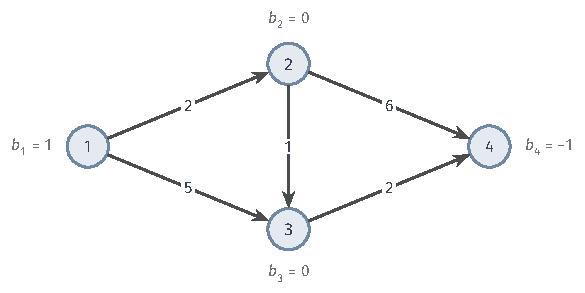
\includegraphics[width=99mm]{figures/05-optimization/01-linear-programming/tikz/lp-network-instance/figure.pdf}
 \caption{一个小网络流实例。弧旁的数字是单位费用$c_{i,j}$，节点旁的$b_i$是净供给：正数表示运出，负数表示收到，零表示只中转。每条弧上的流量$x_{i,j}\geq0$待定。}
 \label{fig:lp-network-instance}
\end{BookInlineFigure}

记弧$(i,j)$上的流量为$x_{i,j}\geq0$。每个节点都要平账：运出的总量减去运入的总量，等于该节点的净供给$b_i$，这称为流量守恒。把五条弧按$(1,2),(1,3),(2,3),(2,4),(3,4)$排列，四个守恒等式合起来就是$\bm{A}\bm{x}=\bm{b}$，其中
\begin{equation}
 \bm{A}=\begin{bmatrix}
 1&1&0&0&0\\
 -1&0&1&1&0\\
 0&-1&-1&0&1\\
 0&0&0&-1&-1
 \end{bmatrix},\qquad
 \bm{b}=\begin{bmatrix}1\\0\\0\\-1\end{bmatrix}.
 \label{eq:lp-network-data}
\end{equation}
$\bm{A}$的每一列对应一条弧，在弧的起点处为$+1$，在终点处为$-1$，其余为零，它是有向图的关联矩阵。

费用向量是$\bm{c}=(2,5,1,6,2)^\top$，总费用$\bm{c}^\top\bm{x}$是线性函数。于是最小费用的运送方案由下面的问题决定：
\[
 \min_{\bm{x}}\ \bm{c}^\top\bm{x}
 \quad\text{s.t.}\quad\bm{A}\bm{x}=\bm{b},\quad\bm{x}\geq\bm{0}.
\]
这里净供给恰好是把一单位货物从节点$1$送到节点$4$，所以问题就是求最短路。若某条弧还有容量上限$x_{i,j}\leq u_{i,j}$，只需多加一条不等式。图上这些问题的专门算法可参考\BookChapterRef{chap:min-cost-flow}{卷三第7章“最小费用流”}，本章只把它们当作线性规划的实例。

\paragraph{标准型}
比较两个模型：资源配置用“$\leq$”约束一般的线性组合，网络流用等式，只把不等号留给单个变量。第二种写法对计算更方便。一组等式可以用线性代数处理，而不等式全部成了“某个坐标非负”，这是最简单的一种不等式。我们把它定为统一的形式。

\begin{definition}[线性规划的标准型]
 \label{def:lp-standard}
 给定$\bm{A}\in\mathbb{R}^{m\times n}$、$\bm{b}\in\mathbb{R}^m$和$\bm{c}\in\mathbb{R}^n$，问题
 \begin{equation}
  \min_{\bm{x}\in\mathbb{R}^n}\ \bm{c}^\top\bm{x}
  \quad\text{s.t.}\quad\bm{A}\bm{x}=\bm{b},\quad\bm{x}\geq\bm{0}
  \label{eq:lp-standard}
 \end{equation}
 称为线性规划的\term{标准型}（standard form），它的可行集记为
 \begin{equation}
  \bm{C}=\{\bm{x}\in\mathbb{R}^n:\bm{A}\bm{x}=\bm{b},\ \bm{x}\geq\bm{0}\}.
  \label{eq:lp-feasible-set}
 \end{equation}
 $\bm{A}$的第$j$列记为$\bm{a}_j=\bm{A}_{:,j}$，最优值记为$p^\star$。
\end{definition}

可以把标准型想成一本账：每个等式是一笔必须平的账，每个变量是一项不能为负的余额。这个比喻只说明约束的形式，并不表示变量都有“余额”的含义。

\paragraph{改写成标准型}
一般的线性规划可以逐项改写。每一步都要说清新旧问题的解怎样相互对应，下面逐种列出。

\emph{最大化改为最小化。}最大化$\bm{p}^\top\bm{x}$与最小化$(-\bm{p})^\top\bm{x}$的最优解相同，最优值互为相反数。

\emph{小于等于约束。}对$\bm{g}^\top\bm{x}\leq h$，引入新变量$s=h-\bm{g}^\top\bm{x}$，约束等价于
\begin{equation}
 \bm{g}^\top\bm{x}+s=h,\qquad s\geq0.
 \label{eq:lp-slack}
\end{equation}
$s$称为\term{松弛变量}（slack variable），它是这条约束还剩的余量。

\emph{大于等于约束。}对$\bm{g}^\top\bm{x}\geq h$，减去\term{剩余变量}（surplus variable）$s=\bm{g}^\top\bm{x}-h\geq0$，得到$\bm{g}^\top\bm{x}-s=h$。

\emph{变量有上下界。}若$x_j\geq l_j$，令$x_j'=x_j-l_j\geq0$；若$x_j\leq u_j$，把它当作一条“小于等于”约束加松弛变量。

\emph{无符号限制的变量。}这样的变量称为\term{自由变量}（free variable）。把它写成两个非负变量之差：
\begin{equation}
 x_j=x_j^{+}-x_j^{-},\qquad x_j^{+}\geq0,\quad x_j^{-}\geq0.
 \label{eq:lp-free-split}
\end{equation}

\begin{example}[车间问题的标准型]
 \label{ex:lp-workshop-standard}
 为工时和原料分别引入松弛变量$x_3,x_4\geq0$，把最大化利润改成最小化利润的相反数，就得到$n=4$，$m=2$的标准型，数据是
 \begin{equation}
  \bm{A}=\begin{bmatrix}1&1&1&0\\2&1&0&1\end{bmatrix},\quad
  \bm{b}=\begin{bmatrix}4\\6\end{bmatrix},\quad
  \bm{c}=\begin{bmatrix}-3\\-2\\0\\0\end{bmatrix}.
  \label{eq:lp-workshop-standard}
 \end{equation}
 第~\ref{chap:optimization}章的解$(x_1,x_2)=(2,2)$对应$\bm{x}=(2,2,0,0)^\top$，工时和原料都恰好用完，目标值是$-10$。
\end{example}

松弛变量的意义可以直接在图上读出。图~\ref{fig:lp-slack-meaning}中，取产量$(1,1)$，代入得到
\[
 x_3=4-1-1=2,\qquad x_4=6-2-1=3.
\]
也就是工时还剩$2$，原料还剩$3$。$x_3=0$恰好是工时约束的边界，$x_3=2$是与边界平行的另一条直线。平面上每个点都对应一组松弛变量的值，点走到哪条边界上，对应的松弛变量就降为零。

\begin{BookInlineFigure}
 \centering
 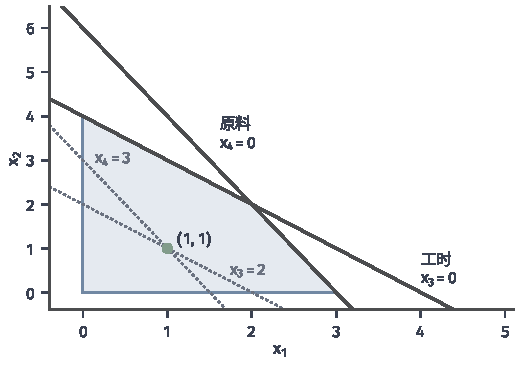
\includegraphics[width=88mm]{figures/05-optimization/01-linear-programming/matplotlib/lp-slack-meaning/figure.pdf}
 \caption{车间问题的松弛变量。深灰粗线是约束取等号的边界，也就是$x_3=0$和$x_4=0$。过绿点$(1,1)$的两条灰色点线是与边界平行的直线，在它们上面$x_3=2$，$x_4=3$，表示这一产量剩下的工时和原料。}
 \label{fig:lp-slack-meaning}
\end{BookInlineFigure}

\paragraph{改写保留了什么}
松弛变量的引入是一一对应的。原问题的可行点$\bm{x}$对应新问题的可行点$(\bm{x},\bm{b}-\bm{A}\bm{x})$，反过来，丢掉松弛变量就回到原来的点。目标值不变，因为松弛变量的费用是零。这个对应是仿射映射，保持线段和中点，所以可行集的形状也保留下来：车间的四边形搬进了$\mathbb{R}^4$，还是同一个四边形。

自由变量的分解不同。从分解后的可行点总能算出原来的$x_j$，目标值相同，所以最优值和最优解的集合不变。但同一个$x_j$有无穷多种写法，图~\ref{fig:lp-free-split}中$(x^{+},x^{-})=(1,0)$和$(3,2)$都表示$x=1$。

\begin{BookInlineFigure}
 \centering
 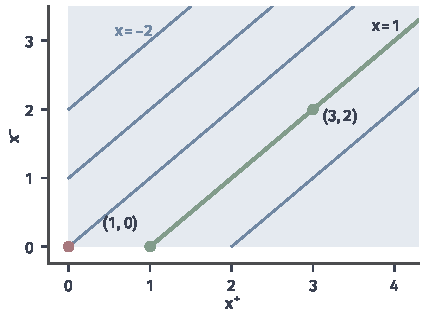
\includegraphics[width=72mm]{figures/05-optimization/01-linear-programming/matplotlib/lp-free-split/figure.pdf}
 \caption{自由变量的分解$x=x^{+}-x^{-}$。浅蓝区域是分解后允许的第一象限，每条斜线上的点代表同一个$x$，绿色粗线是$x=1$。原来的直线变成了一个象限，红点$(0,0)$是这个象限唯一的角点，它在原来的直线上只是普通的一点$x=0$。}
 \label{fig:lp-free-split}
\end{BookInlineFigure}

分解后新问题的最优解可能不唯一，例如沿斜线同时增大$x^{+}$和$x^{-}$，目标值不变。分解还会凭空造出角点：实数轴没有角，第一象限却有角点$(0,0)$。下一节谈顶点时要记住这一点。表~\ref{tab:lp-transformations}汇总了各种改写的效果。

\begin{BookInlineTable}
 \centering
 \begin{tabular}{lll}
  \toprule
  改写 & 解的对应 & 变化 \\
  \midrule
  最大改最小 & 最优解相同 & 最优值变号 \\
  加松弛或剩余变量 & 一一对应 & 变量增加，形状不变 \\
  变量平移 & 一一对应 & 平移可行集 \\
  自由变量分解 & 多对一 & 可能多出角点和最优解 \\
  \bottomrule
 \end{tabular}
 \caption{改写成标准型时各步保留的内容。每一步都保持最优值（或只差符号与常数），并且可以从新问题的解算出原问题的解。}
 \label{tab:lp-transformations}
\end{BookInlineTable}

\paragraph{冗余等式与满行秩}
下一节要从$\bm{A}$中选出可逆的方阵，这需要$\bm{A}$的行没有多余。网络流的矩阵~\eqref{eq:lp-network-data}就有多余的行：每一列恰有一个$+1$和一个$-1$，所以四行相加是零向量，第四行是前三行之和的相反数。$\bm{b}$的分量相加也是零，这说明总供给等于总需求，等式组是相容的。

一般的处理分两步。先检查等式组是否相容，也就是比较$\operatorname{rank}\bm{A}$和增广矩阵的秩：
\[
 \operatorname{rank}\bm{A}=\operatorname{rank}\bigl[\bm{A}\ \ \bm{b}\bigr].
\]
若上式不成立，等式组无解，可行集是空集，问题到此回答完毕。在网络中这对应总供给不等于总需求，货物无处可去。

若相容且$\operatorname{rank}\bm{A}=r<m$，就选出$r$个线性无关的行，其余的行是它们的线性组合，右端也是相应的组合，删去后解集不变。网络的例子里删去第四行即可，剩下三行线性无关，这只要看弧$(1,2),(2,3),(3,4)$三列组成的$3\times3$子矩阵，它是可逆的三角矩阵。秩判别和选主元消元的做法可参考\BookChapterRef{chap:linear-solution-selection}{卷二第11章“线性方程与最小二乘的选解”}。

以后凡涉及基矩阵，都假设已完成这一步，即
\begin{equation}
 \operatorname{rank}\bm{A}=m\leq n.
 \label{eq:lp-full-row-rank}
\end{equation}
车间问题的$\bm{A}$含有单位矩阵，自动满行秩。

\section{基本可行解}
\label{sec:lp-basic-solutions}

线性规划的最优解是否一定落在角点上，角点又怎样用矩阵计算出来？车间问题里这一点靠眼睛看到，变量多了就要靠下面的定义和定理。

\paragraph{多面体与极点}
车间的四边形由四个半平面相交而成。一般地，满足$\bm{g}\neq\bm{0}$的集合$\{\bm{x}:\bm{g}^\top\bm{x}\leq h\}$称为\term{半空间}（halfspace），有限个半空间的交称为\term{多面体}（polyhedron）。写成矩阵形式，就是
\begin{equation}
 \bm{Q}=\{\bm{x}\in\mathbb{R}^n:\bm{G}\bm{x}\leq\bm{h}\},
 \label{eq:lp-polyhedron}
\end{equation}
其中$\bm{G}$的行数有限。等式可以写成两条方向相反的不等式，所以标准型的可行集$\bm{C}$也是多面体。半空间是闭凸集，有限个闭凸集的交仍是闭凸集，多面体因此是闭凸集。

“角点”需要一个不依赖图形的说法。观察图~\ref{fig:lp-extreme-midpoint}：内部的点是某条可行线段的中点，边上的点也是，只不过线段只能沿边摆放。顶点不同，过它的线段无论怎么摆，总有一端跑到可行集外面。

\begin{BookInlineFigure}
 \centering
 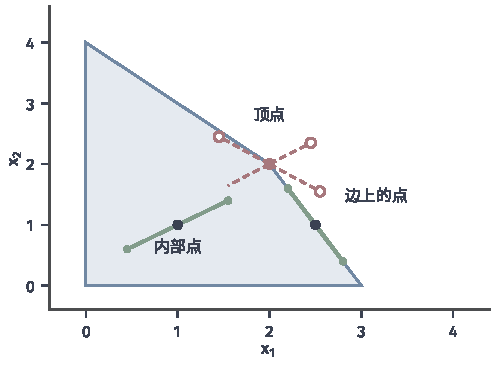
\includegraphics[width=84mm]{figures/05-optimization/01-linear-programming/matplotlib/lp-extreme-midpoint/figure.pdf}
 \caption{三种位置的点。深色的内部点和边上的点都是一条可行线段（绿色）的中点。红点$(2,2)$是顶点，过它的线段（红色虚线）总有一端落在四边形外（空心点），所以它不是任何可行线段的中点。}
 \label{fig:lp-extreme-midpoint}
\end{BookInlineFigure}

\begin{definition}[极点]
 \label{def:lp-extreme-point}
 设$\bm{Q}$是凸集，$\bm{x}\in\bm{Q}$。若$\bm{u},\bm{v}\in\bm{Q}$且$\bm{x}=(\bm{u}+\bm{v})/2$只有在$\bm{u}=\bm{v}=\bm{x}$时才成立，就称$\bm{x}$是$\bm{Q}$的\term{极点}（extreme point）。
\end{definition}

对多面体，极点也称为顶点，本章两种说法通用。

\paragraph{基与基本解}
标准型的可行点要满足$m$个等式，却有$n$个未知数，还剩$n-m$个自由度。平面上的顶点是让两条约束同时取等号得到的，在标准型里，取等号的办法是让坐标变成零。于是自然的做法是：让$n-m$个坐标取零，用$m$个等式解出其余$m$个坐标。

能否解出，取决于留下的那$m$列是否线性无关。

\begin{definition}[基与基本可行解]
 \label{def:lp-basic-solution}
 设$\bm{A}$满行秩。取$m$个下标组成集合$B$，其余下标组成$N$。若由$B$中各列构成的方阵$\bm{A}_B$可逆，就称$B$为一个基，$\bm{A}_B$为\term{基矩阵}（basis matrix）。令
 \begin{equation}
  \bm{x}_B=\bm{A}_B^{-1}\bm{b},\qquad\bm{x}_N=\bm{0},
  \label{eq:lp-basic-solution}
 \end{equation}
 所得的$\bm{x}$称为基$B$对应的\term{基本解}（basic solution），$\bm{x}_B$和$\bm{x}_N$的分量分别称为基分量和非基分量。若还有$\bm{x}_B\geq\bm{0}$，就称$\bm{x}$为\term{基本可行解}（basic feasible solution），$B$为可行基。
\end{definition}

基本解满足全部等式，但不一定非负，所以不一定可行。在车间问题~\eqref{eq:lp-workshop-standard}中，$\bm{A}$的四列任取两列都线性无关，共有$\binom{4}{2}=6$个基。以$B=\{1,4\}$为例，令$x_2=x_3=0$，两个等式变成
\[
 x_1=4,\qquad 2x_1+x_4=6.
\]
解得$x_1=4$，$x_4=-2$。分量为负，这个基本解不可行：产量$(4,0)$用掉的原料比库存多$2$。表~\ref{tab:lp-six-bases}列出了全部六个基本解。

\begin{BookInlineTable}
 \centering
 \begin{tabular}{cccc}
  \toprule
  基$B$ & $\bm{x}=(x_1,x_2,x_3,x_4)$ & 平面上的点 & 是否可行\\
  \midrule
  $\{3,4\}$ & $(0,0,4,6)$ & $(0,0)$ & 可行\\
  $\{1,3\}$ & $(3,0,1,0)$ & $(3,0)$ & 可行\\
  $\{2,4\}$ & $(0,4,0,2)$ & $(0,4)$ & 可行\\
  $\{1,2\}$ & $(2,2,0,0)$ & $(2,2)$ & 可行\\
  $\{1,4\}$ & $(4,0,0,-2)$ & $(4,0)$ & 不可行\\
  $\{2,3\}$ & $(0,6,-2,0)$ & $(0,6)$ & 不可行\\
  \bottomrule
 \end{tabular}
 \caption{车间问题的六个基本解。可行的四个恰好是四边形的四个顶点。}
 \label{tab:lp-six-bases}
\end{BookInlineTable}

图~\ref{fig:lp-basic-solutions}把这六个点画在平面上。它们正是四条边界直线的两两交点：选定基，就是选定哪两个坐标取零，也就是选定哪两条边界同时取等号。

\begin{BookInlineFigure}
 \centering
 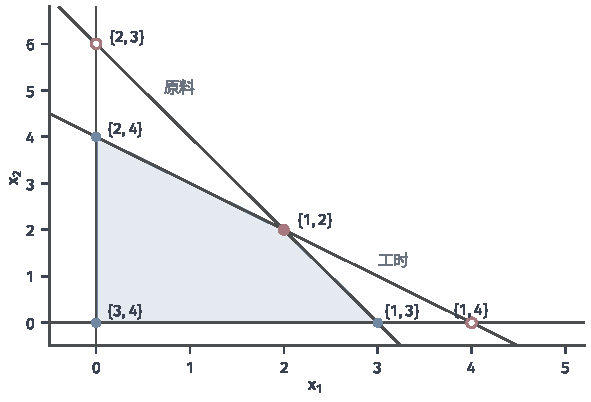
\includegraphics[width=100mm]{figures/05-optimization/01-linear-programming/matplotlib/lp-basic-solutions/figure.pdf}
 \caption{车间问题的六个基本解，点旁标出对应的基。四条直线是$x_1=0$、$x_2=0$和工时、原料两条约束的边界。实心点是四个基本可行解，其中红点$(2,2)$最优；红色空心点$(4,0)$和$(0,6)$的基本解有负分量，落在可行域外。}
 \label{fig:lp-basic-solutions}
\end{BookInlineFigure}

\paragraph{基本可行解就是极点}
表中四个可行的基本解恰好是四个顶点，这不是巧合。下面的定理把代数对象和几何对象连起来，判别的依据是矩阵的秩：只看正分量所在的列。

\begin{theorem}[基本可行解与极点]
 \label{thm:lp-bfs-extreme}
 设$\bm{A}$满行秩，$\bm{x}\in\bm{C}$，$J=\{j:x_j>0\}$。下面三条等价：
 \begin{enumerate}
  \item $\bm{x}$是$\bm{C}$的极点；
  \item 列$\{\bm{a}_j:j\in J\}$线性无关；
  \item $\bm{x}$是某个基对应的基本可行解。
 \end{enumerate}
\end{theorem}

\begin{proof}
 先证(1)推出(2)。假设这些列线性相关，则有不全为零的系数$w_j$（$j\in J$）使$\sum_{j\in J}w_j\bm{a}_j=\bm{0}$。把$\bm{w}$在$J$以外的分量补成零，就有
 \[
  \bm{A}\bm{w}=\bm{0},\qquad\bm{w}\neq\bm{0}.
 \]
 $J$上的$x_j$都是正数，取足够小的$\varepsilon>0$，可使$\bm{x}\pm\varepsilon\bm{w}\geq\bm{0}$。再由$\bm{A}\bm{w}=\bm{0}$知这两个点都满足等式，都可行。它们不相等，而$\bm{x}$是它们的中点，与$\bm{x}$是极点矛盾。

 再证(2)推出(3)。线性无关的列不超过$m$个，所以$\lvert J\rvert\leq m$。$\bm{A}$满行秩，它的列张成$\mathbb{R}^m$，可以再补入若干列，把$\{\bm{a}_j:j\in J\}$扩充成$\mathbb{R}^m$的一组基，相应的下标集记为$B\supseteq J$。于是$\bm{A}_B$可逆，$B$之外的分量都不在$J$中，所以$\bm{x}_N=\bm{0}$。代入等式得到
 \[
  \bm{A}_B\bm{x}_B=\bm{b},\qquad\text{即}\qquad\bm{x}_B=\bm{A}_B^{-1}\bm{b}.
 \]
 又$\bm{x}$可行，故$\bm{x}_B\geq\bm{0}$，它是基$B$的基本可行解。

 最后证(3)推出(1)。设$\bm{x}$是基$B$的基本可行解，且$\bm{x}=(\bm{u}+\bm{v})/2$，$\bm{u},\bm{v}\in\bm{C}$。对$j\in N$，有$u_j+v_j=2x_j=0$，又$u_j,v_j\geq0$，所以$u_j=v_j=0$。于是$\bm{A}_B\bm{u}_B=\bm{b}$，由$\bm{A}_B$可逆得到
 \[
  \bm{u}_B=\bm{A}_B^{-1}\bm{b}=\bm{x}_B.
 \]
 所以$\bm{u}=\bm{x}$，同理$\bm{v}=\bm{x}$。
\end{proof}

定理中的秩条件有直接的几何解释。在点$\bm{x}$处取等号的约束是$m$个等式和$n-\lvert J\rvert$个“坐标为零”。把它们的系数排成矩阵$\bm{M}$，$\bm{M}\bm{v}=\bm{0}$说的是
\[
 \bm{v}_{J^c}=\bm{0},\qquad\bm{A}_J\bm{v}_J=\bm{0}.
\]
其中$J^c$是$J$的补集。所以$\bm{M}$的列满秩，也就是取等号的约束能唯一确定一个点，当且仅当$\bm{A}_J$的列线性无关。“$n$个线性无关的约束取等号”和“基矩阵可逆”是同一件事的两种说法。

用车间问题验证一下。点$(5/2,1)$对应$\bm{x}=(5/2,1,1/2,0)^\top$，正分量在第$1,2,3$列，三列放在$\mathbb{R}^2$中线性相关，取
\[
 \bm{w}=(-1,2,-1,0)^\top,\qquad\bm{A}\bm{w}=\bm{0}.
\]
$\bm{x}\pm\varepsilon\bm{w}$都可行，所以它不是极点，在图上它是原料边界中间的一点。点$(2,2)$对应$\bm{x}=(2,2,0,0)^\top$，第$1,2$列线性无关，它是极点。

基的个数不超过$\binom{n}{m}$，所以极点只有有限个。最优解若能在极点取得，问题就从无穷多个候选变成了有限多个。

\paragraph{最优解可以在基本可行解中取得}
下面证明这确实成立。证明的想法很具体：任取一个可行点，如果它的正分量对应的列线性相关，就有一个方向可以沿着走，目标不变差，直到某个正分量降到零。正分量越来越少，最后得到一个基本可行解。

\begin{lemma}[推向基本可行解]
 \label{lem:lp-push}
 设$\bm{A}$满行秩，且$\bm{c}^\top\bm{x}$在$\bm{C}$上有下界。则对每个$\bm{x}\in\bm{C}$，存在基本可行解$\widehat{\bm{x}}$，使
 \begin{equation}
  \bm{c}^\top\widehat{\bm{x}}\leq\bm{c}^\top\bm{x}.
  \label{eq:lp-push}
 \end{equation}
\end{lemma}

\begin{proof}
 对正分量的个数$\lvert J\rvert$归纳。若列$\{\bm{a}_j:j\in J\}$线性无关，由定理~\ref{thm:lp-bfs-extreme}，$\bm{x}$本身就是基本可行解。

 否则取$\bm{w}\neq\bm{0}$，满足$\bm{A}\bm{w}=\bm{0}$，且$w_j=0$对$j\notin J$成立。必要时用$-\bm{w}$代替$\bm{w}$，可使$\bm{c}^\top\bm{w}\leq0$。先说明可以假设$\bm{w}$有负分量。

 若$\bm{w}\geq\bm{0}$且$\bm{c}^\top\bm{w}<0$，则对一切$t\geq0$，点$\bm{x}+t\bm{w}$可行，目标值$\bm{c}^\top\bm{x}+t\bm{c}^\top\bm{w}$趋于$-\infty$，与有下界矛盾，这种情形不出现。若$\bm{w}\geq\bm{0}$且$\bm{c}^\top\bm{w}=0$，就把$\bm{w}$换成$-\bm{w}$，此时$\bm{c}^\top\bm{w}$仍为零，而$\bm{w}$有了负分量。

 现在令
 \[
  t^\star=\min_{j:\,w_j<0}\frac{x_j}{-w_j},\qquad\bm{x}'=\bm{x}+t^\star\bm{w}.
 \]
 负分量只出现在$J$中，那里$x_j>0$，所以$t^\star>0$。$t^\star$的取法保证$\bm{x}'\geq\bm{0}$，又$\bm{A}\bm{x}'=\bm{b}$，所以$\bm{x}'$可行，并且
 \[
  \bm{c}^\top\bm{x}'=\bm{c}^\top\bm{x}+t^\star\bm{c}^\top\bm{w}\leq\bm{c}^\top\bm{x}.
 \]

 $J$之外的分量保持为零，取到最小值的分量变成零，所以$\bm{x}'$的正分量个数严格减少。对$\bm{x}'$用归纳假设，即得$\widehat{\bm{x}}$。
\end{proof}

用车间问题走一遍。从可行点$(x_1,x_2)=(1,1)$出发，四个坐标是$\bm{x}=(1,1,2,3)^\top$，目标值$-5$。四列放在$\mathbb{R}^2$中必然线性相关，可以取下面的方向，并算出步长：
\[
 \bm{w}=(1,0,-1,-2)^\top,\qquad\bm{c}^\top\bm{w}=-3,\qquad
 t^\star=\min\Bigl\{\frac{2}{1},\frac{3}{2}\Bigr\}=\frac32.
\]
走完得到第一个新点，$x_4$降到了零：
\[
 \bm{x}'=\Bigl(\frac52,1,\frac12,0\Bigr)^\top,\qquad\bm{c}^\top\bm{x}'=-\frac{19}{2}.
\]

此时还剩三个正分量，第$1,2,3$列在$\mathbb{R}^2$中仍然线性相关。满足$w_4=0$的零空间方向是$(1,-2,1,0)^\top$，它的目标变化率是$+1$，所以取反方向，并求步长：
\[
 \bm{w}=(-1,2,-1,0)^\top,\qquad\bm{c}^\top\bm{w}=-1,\qquad
 t^\star=\min\Bigl\{\frac{5/2}{1},\frac{1/2}{1}\Bigr\}=\frac12.
\]
走完得到
\[
 \bm{x}''=(2,2,0,0)^\top,\qquad\bm{c}^\top\bm{x}''=-10.
\]
正分量只剩两个，对应的列线性无关，这就是基本可行解。图~\ref{fig:lp-push-to-vertex}显示了这两步：先水平走到原料边界，再沿边界走到顶点。这里碰巧到达了最优解，一般只能保证目标不变差。

\begin{BookInlineFigure}
 \centering
 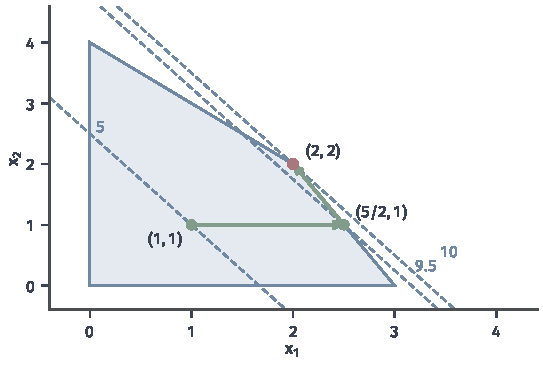
\includegraphics[width=92mm]{figures/05-optimization/01-linear-programming/matplotlib/lp-push-to-vertex/figure.pdf}
 \caption{引理~\ref{lem:lp-push}在车间问题上的两步。绿色箭头从$(1,1)$（四个正分量）走到$(5/2,1)$（三个正分量），再走到顶点$(2,2)$（两个正分量）。蓝色虚线是利润等于$5$、$9.5$、$10$的等值线，每一步都不使利润变小。}
 \label{fig:lp-push-to-vertex}
\end{BookInlineFigure}

\begin{theorem}[最优基本可行解的存在]
 \label{thm:lp-optimal-bfs}
 设$\bm{A}$满行秩。若标准型~\eqref{eq:lp-standard}可行且最优值有限，则最优值能够取到，并且至少有一个最优解是基本可行解。特别地，非空的$\bm{C}$至少有一个极点。
\end{theorem}

\begin{proof}
 基本可行解至多有$\binom{n}{m}$个，由引理~\ref{lem:lp-push}（对$\bm{C}$中任一点使用），它们至少有一个。在这有限个点中取目标值最小的$\bm{x}^\star$。对任意$\bm{x}\in\bm{C}$，引理给出基本可行解$\widehat{\bm{x}}$，于是
 \[
  \bm{c}^\top\bm{x}\geq\bm{c}^\top\widehat{\bm{x}}\geq\bm{c}^\top\bm{x}^\star.
 \]
 所以$\bm{x}^\star$是最优解。最后一句取$\bm{c}=\bm{0}$即得。
\end{proof}

定理中“$\bm{A}$满行秩”只是为了让基有定义，这一点上一节已经保证。这个结论比一般的存在定理强。第~\ref{chap:optimization}章的$e^x$有下界却取不到下确界，而标准型线性规划只要最优值有限，就一定取得到，并不要求可行集有界。条件里的“可行”和“最优值有限”各自排除一种结局，图~\ref{fig:lp-three-outcomes}画出了线性规划的三种情形。

\begin{BookInlineFigure}
 \centering
 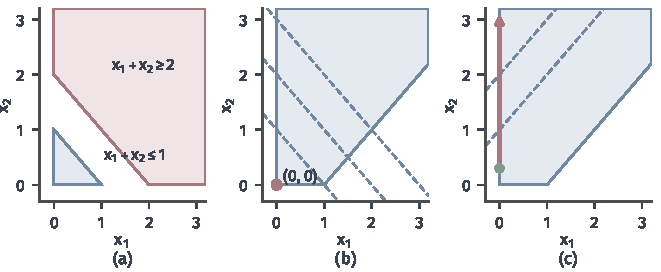
\includegraphics[width=112mm]{figures/05-optimization/01-linear-programming/matplotlib/lp-three-outcomes/figure.pdf}
 \caption{线性规划的三种结局。(a)~第一象限中两条约束围成的区域不相交，问题不可行。(b)~可行域$\{\bm{x}\geq\bm{0},\ x_1-x_2\leq1\}$无界，但最小化$x_1+x_2$（蓝色虚线是等值线）的最优解存在，是红点$(0,0)$。(c)~同一可行域上最小化$x_1-x_2$，从绿点沿红色射线一直走，目标趋于$-\infty$，问题无下界。}
 \label{fig:lp-three-outcomes}
\end{BookInlineFigure}

定理只说有一个最优解是基本可行解，不说所有最优解都是。把车间的目标改成最大化$2x_1+x_2$，等值线与原料边界平行，图~\ref{fig:lp-optimal-face}(b)中$(2,2)$和$(3,0)$都最优，它们连线上的每一点也都最优。中点$(5/2,1)$对应$\bm{x}=(5/2,1,1/2,0)^\top$，有三个正分量，多于$m=2$，所以不是基本可行解，却同样最优。

\begin{BookInlineFigure}
 \centering
 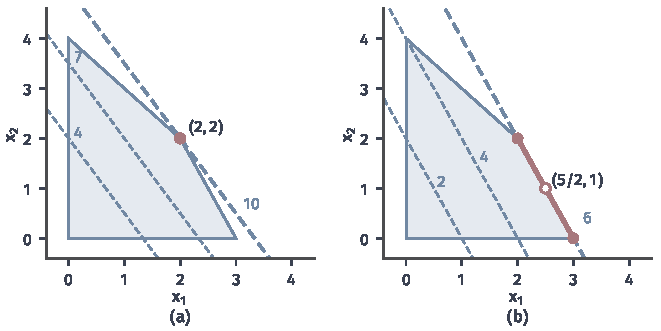
\includegraphics[width=112mm]{figures/05-optimization/01-linear-programming/matplotlib/lp-optimal-face/figure.pdf}
 \caption{等值线平移到最后接触可行域的情形。(a)~最大化$3x_1+2x_2$，粗虚线（利润$10$）只接触顶点$(2,2)$，最优解唯一。(b)~最大化$2x_1+x_2$，粗虚线（值为$6$）与一条边重合，红色线段上都是最优解，其中空心点$(5/2,1)$不是顶点。}
 \label{fig:lp-optimal-face}
\end{BookInlineFigure}

定理把问题化成了有限比较，但枚举全部的基并不现实。$n=100$，$m=50$时，$\binom{n}{m}$约为$1.0\times10^{29}$。需要的是一种不逐个检查、只在相邻顶点之间移动的办法，下面先说清“相邻”是什么意思。

\paragraph{沿边到相邻顶点}
在车间的四边形上，相邻顶点由一条边相连。用基来说，相邻的两个基只差一个下标。设$B$是可行基，$\bar{\bm{x}}$是它的基本可行解，取一个不在$B$中的下标$q$。让$x_q$从零增大，其余非基分量保持为零，基分量必须随之调整，以维持等式。由$\bm{A}_B\bm{x}_B+\bm{a}_qx_q=\bm{b}$解出
\begin{equation}
 \bm{x}_B=\bar{\bm{x}}_B-x_q\bm{u},\qquad\bm{u}=\bm{A}_B^{-1}\bm{a}_q.
 \label{eq:lp-edge-direction}
\end{equation}
这相当于让点沿方向$\bm{d}$移动，其中$d_q=1$，$\bm{d}_B=-\bm{u}$，其余分量为零，并且$\bm{A}\bm{d}=\bm{0}$。

\begin{theorem}[沿边的移动]
 \label{thm:lp-edge-move}
 设$\bm{A}$满行秩，$B$是可行基，$\bar{\bm{x}}$是其基本可行解，$q\notin B$，$\bm{u}$和$\bm{d}$如上。则满足“$x_j=0$对$j\notin B\cup\{q\}$成立”的可行点恰好是$\bar{\bm{x}}+\alpha\bm{d}$，其中$\alpha\geq0$且$\bar{\bm{x}}_B-\alpha\bm{u}\geq\bm{0}$。进一步：
 \begin{enumerate}
  \item 若$\bm{u}$有正分量，且$\bar{\bm{x}}_B>\bm{0}$，记$r$是下式取到最小值的位置，$B(i)$是基中第$i$个下标：
  \begin{equation}
   \alpha^\star=\min_{i:\,u_i>0}\frac{\bar{x}_{B(i)}}{u_i}>0.
   \label{eq:lp-edge-step}
  \end{equation}
  把$B$中的$B(r)$换成$q$得到新基，$\bar{\bm{x}}+\alpha^\star\bm{d}$是新基的基本可行解，且与$\bar{\bm{x}}$不同。
  \item 若$\bm{u}\leq\bm{0}$，则对一切$\alpha\geq0$，$\bar{\bm{x}}+\alpha\bm{d}$都可行。
 \end{enumerate}
\end{theorem}

\begin{proof}
 由式~\eqref{eq:lp-edge-direction}，满足等式且$x_j=0$（$j\notin B\cup\{q\}$）的点完全由$x_q$确定，就是$\bar{\bm{x}}+x_q\bm{d}$。再加上非负条件，得到第一句。

 对情形1，$\bar{\bm{x}}_B>\bm{0}$保证$\alpha^\star>0$，点因此确实移动了。$\alpha^\star$的取法使基分量保持非负，而位置$r$上的分量降为零。新基矩阵可逆：由$\bm{A}_B\bm{u}=\bm{a}_q$，有$\bm{a}_q=\sum_iu_i\bm{a}_{B(i)}$，其中$\bm{a}_{B(r)}$的系数$u_r\neq0$，所以用$\bm{a}_q$替换$\bm{a}_{B(r)}$后列仍线性无关。新点在新基之外的分量都是零，它就是新基的基本可行解。

 对情形2，$\bm{u}\leq\bm{0}$时基分量不减，$\alpha\geq0$都满足非负条件。
\end{proof}

定理的第一句就是“边”的代数含义：$m$个等式和$n-m-1$个坐标为零，共$n-1$个线性无关的条件，只留下一个自由度，可行点构成一条线段或射线。把一个下标换入、另一个换出，这个操作称为换基，它的几何含义在基分量都为正时正是沿边走到相邻顶点。选哪个$q$能改善目标，是第~\ref{chap:simplex-method}章的问题，这里只看移动本身。

在车间问题上从$B=\{3,4\}$，即点$(0,0)$出发，让$x_1$增大。此时$\bm{A}_B=\bm{I}$，于是
\[
 \bm{u}=\bm{a}_1=\begin{bmatrix}1\\2\end{bmatrix},\qquad
 \bar{\bm{x}}_B=\begin{bmatrix}4\\6\end{bmatrix},\qquad
 \alpha^\star=\min\Bigl\{\frac41,\frac62\Bigr\}=3.
\]
最小值由原料的松弛变量$x_4$取到，所以$x_4$换出，点沿下边走到$(3,0)$，新基是$\{1,3\}$，其中基分量$x_1=3$，$x_3=4-3=1$。

再让$x_2$增大。新基矩阵的列是$\bm{a}_1,\bm{a}_3$，解$\bm{A}_B\bm{u}=\bm{a}_2$，并按位置比较：
\[
 \bm{u}=\begin{bmatrix}1/2\\1/2\end{bmatrix},\qquad
 \bar{\bm{x}}_B=\begin{bmatrix}3\\1\end{bmatrix},\qquad
 \alpha^\star=\min\Bigl\{\frac{3}{1/2},\frac{1}{1/2}\Bigr\}=2.
\]
$x_3$先降到零，$x_1$变成$3-2\cdot\frac12=2$，$x_2$变成$2$，点走到$(2,2)$，基变成$\{1,2\}$。图~\ref{fig:lp-pivot-edge}显示了这两次移动和第一次移动中基分量的变化。基$\{3,4\}$和$\{1,2\}$差两个下标，它们的顶点$(0,0)$与$(2,2)$不相邻，连接它们的线段穿过四边形内部，不是边。

\begin{BookInlineFigure}
 \centering
 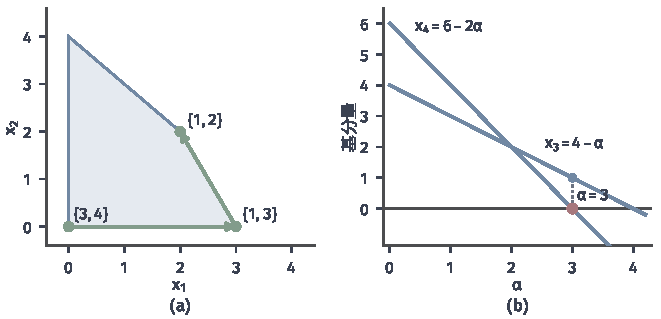
\includegraphics[width=112mm]{figures/05-optimization/01-linear-programming/matplotlib/lp-pivot-edge/figure.pdf}
 \caption{两次换基。(a)~绿色箭头沿边从$(0,0)$到$(3,0)$，再到$(2,2)$，点旁是当时的基。(b)~第一次移动时两个基分量随步长$\alpha$下降，$x_4$在$\alpha=3$处最先到零（红点），此时$x_3=1$。}
 \label{fig:lp-pivot-edge}
\end{BookInlineFigure}

\paragraph{含直线的多面体没有极点}
以上结论都是对标准型说的。它们能推广到什么范围？在平面上考虑带形
\[
 \{(x_1,x_2):0\leq x_2\leq1\}.
\]
最小化$x_2$，最优值$0$在整条直线$x_2=0$上取得，但这个集合没有角点。图~\ref{fig:lp-no-vertex-strip}(a)中，每个点都是左右两个可行点的中点。可见“有最优解就有最优顶点”不是所有多面体都有的性质，缺的是下面的秩条件。

\begin{BookInlineFigure}
 \centering
 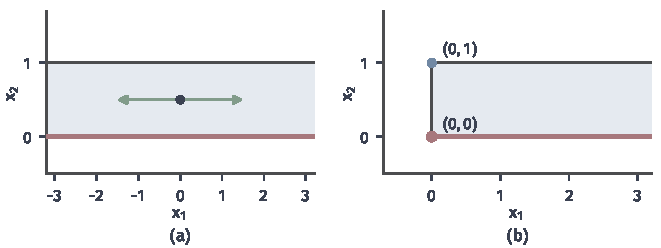
\includegraphics[width=112mm]{figures/05-optimization/01-linear-programming/matplotlib/lp-no-vertex-strip/figure.pdf}
 \caption{极点的存在依赖可行集的形状，目标取$x_2$，红色粗线是最优解集合。(a)~带形含有水平直线，绿色线段说明任一点都是两个可行点的中点，所以没有极点，最优解集合也没有端点。(b)~加上$x_1\geq0$后不再含直线，出现顶点$(0,0)$和$(0,1)$，最优值在顶点$(0,0)$取得。}
 \label{fig:lp-no-vertex-strip}
\end{BookInlineFigure}

\begin{lemma}[多面体的极点]
 \label{lem:lp-polyhedron-vertices}
 设$\bm{Q}=\{\bm{x}:\bm{G}\bm{x}\leq\bm{h}\}$非空，其中$\bm{G}$有$n$列。对$\bm{x}\in\bm{Q}$，记$I(\bm{x})$为取等号的行的下标集。则$\bm{x}$是极点，当且仅当$\bm{G}_{I(\bm{x}),:}$的秩为$n$。进一步，下面三条等价：$\bm{Q}$有极点；$\operatorname{rank}\bm{G}=n$；$\bm{Q}$不含直线。
\end{lemma}

\begin{proof}
 先证第一句。若取等号的行的秩小于$n$，存在$\bm{d}\neq\bm{0}$使这些行与$\bm{d}$的内积都为零。其余的行留有余量，$\varepsilon>0$足够小时$\bm{x}\pm\varepsilon\bm{d}\in\bm{Q}$，所以$\bm{x}$不是极点。反之设秩为$n$，且$\bm{x}=(\bm{u}+\bm{v})/2$，$\bm{u},\bm{v}\in\bm{Q}$。对每个$i\in I(\bm{x})$，两个不超过$h_i$的数平均后等于$h_i$，只能都等于$h_i$，所以$\bm{u}$和$\bm{v}$满足相同的取等号方程组。这个方程组的解唯一，故$\bm{u}=\bm{v}=\bm{x}$。

 再证三条等价。若$\operatorname{rank}\bm{G}<n$，取$\bm{d}\neq\bm{0}$使$\bm{G}\bm{d}=\bm{0}$，则过任一点沿$\bm{d}$的直线都在$\bm{Q}$中，这时由第一句也没有极点。反之若$\bm{Q}$含直线$\bm{x}+t\bm{d}$，则对全部$t\in\mathbb{R}$有$\bm{G}(\bm{x}+t\bm{d})\leq\bm{h}$，只能$\bm{G}\bm{d}=\bm{0}$，秩小于$n$。若有极点，由第一句$\bm{G}$的秩为$n$。

 剩下要证$\operatorname{rank}\bm{G}=n$时有极点。取$\bm{Q}$中使$\operatorname{rank}\bm{G}_{I(\bm{x}),:}$最大的点$\bm{x}$。假设这个秩小于$n$，取$\bm{d}\neq\bm{0}$与取等号的行都正交。由$\operatorname{rank}\bm{G}=n$，$\bm{G}\bm{d}\neq\bm{0}$，必要时换成$-\bm{d}$，可设有一行的内积为正。沿$\bm{d}$走到第一条新约束取等号为止，原来取等号的行仍取等号，新行与$\bm{d}$不正交，不在原来那些行的张成中，秩增大，矛盾。所以这个秩等于$n$，$\bm{x}$是极点。
\end{proof}

标准型中$\bm{G}$含有$-\bm{I}$这一块，秩一定是$n$，所以非负约束自动排除了直线。定理~\ref{thm:lp-optimal-bfs}成立的前提正是这一点。

上一节说自由变量分解会造出角点，这里可以看得很清楚。把带形写成标准型：令$x_1=x_1^{+}-x_1^{-}$，加松弛变量$w$，约束只剩一个等式$x_2+w=1$。基只能是$\{x_2\}$或$\{w\}$，基$\{w\}$给出的基本可行解$(x_1^{+},x_1^{-},x_2,w)=(0,0,0,1)$是最优的。它对应带形中的点$(0,0)$，这个点是最优解，却不是带形的顶点。所以应用定理时要分清：顶点是标准型的顶点，回到原问题后只保证是一个最优解。

\paragraph{退化基与无界可行方向}
基和点的对应还有两种偏差，表现相似，含义却不同，都发生在换基的时候。

第一种是几个基对应同一个点。给车间问题再加一条约束$x_1\leq3$，引入松弛变量$x_5$，得到$m=3$，$n=5$的标准型。可行域没有变化，但顶点$(3,0)$现在有三条边界经过，如图~\ref{fig:lp-degenerate-vertex}。这个点是
\[
 \bm{x}=(3,0,1,0,0)^\top,
\]
只有$x_1,x_3$两个正分量，而基需要三个下标。

\begin{BookInlineFigure}
 \centering
 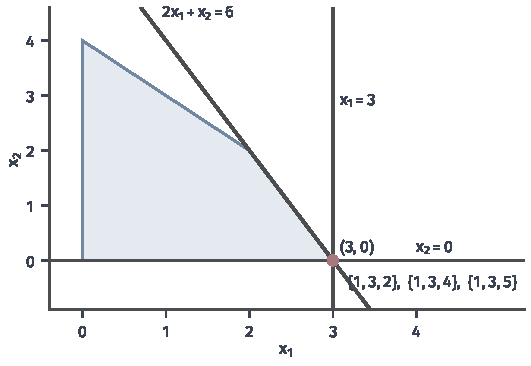
\includegraphics[width=90mm]{figures/05-optimization/01-linear-programming/matplotlib/lp-degenerate-vertex/figure.pdf}
 \caption{退化顶点。加入约束$x_1\leq3$后，四边形没有变，但三条深灰粗线同时经过红点$(3,0)$。第三个基下标取$2$、$4$或$5$，三个基$\{1,3,2\}$、$\{1,3,4\}$、$\{1,3,5\}$都给出这同一个点。}
 \label{fig:lp-degenerate-vertex}
\end{BookInlineFigure}

第三个下标可以取$2$、$4$或$5$，三个基矩阵都可逆，所以三个基给出同一个点，每个基中都有一个取零的基分量。这样的基称为\term{退化基}（degenerate basis），对应的基本可行解称为退化的。此时定理~\ref{thm:lp-edge-move}的条件$\bar{\bm{x}}_B>\bm{0}$不成立。

从基$\{1,3,2\}$（基分量依次为$3,1,0$）出发，让$x_4$增大，解$\bm{A}_B\bm{u}=\bm{a}_4$得到
\[
 \bm{u}=(0,-1,1)^\top,\qquad\alpha^\star=\frac{0}{1}=0.
\]
基变成$\{1,3,4\}$，点却一动不动。“换基”和“走到另一个顶点”在退化时不再是一回事。

第二种是沿某条边可以走到无穷远。取可行域$x_1-x_2\leq1$，$\bm{x}\geq\bm{0}$，写成标准型$x_1-x_2+x_3=1$，这里$m=1$。在基$\{3\}$处，点是$(0,0,1)^\top$。让$x_2$增大：
\[
 u=\bm{A}_B^{-1}\bm{a}_2=-1\leq0.
\]
由定理~\ref{thm:lp-edge-move}的情形2，沿$\bm{d}=(0,1,1)^\top$可以一直走。满足下面条件的$\bm{d}$称为\term{无界可行方向}（unbounded feasible direction）：
\begin{equation}
 \bm{A}\bm{d}=\bm{0},\qquad\bm{d}\geq\bm{0},\qquad\bm{d}\neq\bm{0}.
 \label{eq:lp-recession}
\end{equation}
任何可行点沿它走都不会离开$\bm{C}$。这是可行集形状的性质，与目标无关：可行集无界不等于问题无下界，只有$\bm{c}^\top\bm{d}<0$时目标才沿它趋于$-\infty$。图~\ref{fig:lp-three-outcomes}的(b)与(c)用的正是同一个可行域。表~\ref{tab:lp-degenerate-vs-ray}对比了这两种现象。

\begin{BookInlineTable}
 \centering
 \begin{tabular}{lll}
  \toprule
  & 退化基 & 无界可行方向 \\
  \midrule
  代数表现 & 基分量取零 & $\bm{u}\leq\bm{0}$ \\
  步长 & 可能$\alpha^\star=0$ & 没有上限 \\
  几何含义 & 多余约束过同一顶点 & 可行集沿射线无界 \\
  对目标的影响 & 换基后点和目标值不变 & $\bm{c}^\top\bm{d}<0$时无下界 \\
  \bottomrule
 \end{tabular}
 \caption{退化基与无界可行方向的对比。}
 \label{tab:lp-degenerate-vs-ray}
\end{BookInlineTable}

\section{线性规划的对偶}
\label{sec:lp-duality}

有人告诉我们，车间问题的最优解是$(2,2)$，最大利润是$10$。检查可行性只需代入约束，难的是确认没有更好的产量。怎样给出一份不依赖求解过程、能当场核对的最优性证据？答案来自第~\ref{chap:optimization}章用过的办法，把约束加起来，只是这次要系统地做。

\paragraph{给约束配权重}
把工时约束乘以$u_1\geq0$，原料约束乘以$u_2\geq0$，再相加。权重非负，不等号方向不变，得到
\[
 (u_1+2u_2)x_1+(u_1+u_2)x_2\leq4u_1+6u_2.
\]
如果左边的系数“盖得住”利润系数，也就是
\[
 u_1+2u_2\geq3,\qquad u_1+u_2\geq2,
\]
那么由$x_1,x_2\geq0$，任何可行产量的利润都不超过$4u_1+6u_2$。

不同的权重给出不同的上界。下面四组权重都满足上述条件：
\[
 \bm{u}=(2,1)\to14,\quad(3,0)\to12,\quad(0,2)\to12,\quad(1,1)\to10.
\]
最后一个上界$10$恰好等于$(2,2)$的利润，所以$(2,2)$最优。这一行计算不依赖任何算法，谁都可以复核。

权重可以读成资源的价格。设想有人想买下车间全部的工时和原料，出价$u_1,u_2$。车间只在卖资源不比自己生产亏时才肯卖，这就是上面的两个不等式。买方希望总价$4u_1+6u_2$尽量低，寻找最低总价就是寻找最紧的上界，于是有问题
\begin{equation}
 \min_{u_1,u_2}\ 4u_1+6u_2
 \quad\text{s.t.}\quad u_1+2u_2\geq3,\quad u_1+u_2\geq2,\quad u_1,u_2\geq0.
 \label{eq:lp-workshop-prices}
\end{equation}
图~\ref{fig:lp-dual-bounds}(a)是这个问题的可行域，最低总价$10$在$(1,1)$取得。图~\ref{fig:lp-dual-bounds}(b)把两边的数放在同一条数轴上：每个产量的利润都在每个价格的总价左边，两者在$10$处相遇。这正是“上下界夹逼”。买卖的故事只用来说明不等式的方向，并不表示真有这样一个市场，价格只是一组使不等式成立的数。

\begin{BookInlineFigure}
 \centering
 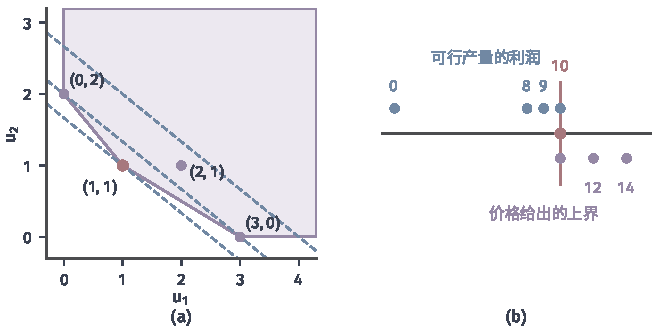
\includegraphics[width=112mm]{figures/05-optimization/01-linear-programming/matplotlib/lp-dual-bounds/figure.pdf}
 \caption{资源价格给出的上界。(a)~浅紫区域是满足式~\eqref{eq:lp-workshop-prices}约束的价格$(u_1,u_2)$，蓝色虚线是总价$10,12,16$的等值线，红点$(1,1)$是最低总价。(b)~数轴上方的蓝点是四个顶点的利润$0,8,9,10$，下方的紫点是四组价格的总价$10,12,14$，红线标出两侧在$10$处相遇。}
 \label{fig:lp-dual-bounds}
\end{BookInlineFigure}

\paragraph{标准型的对偶问题}
对标准型~\eqref{eq:lp-standard}做同样的事。约束是等式，乘以任意实数都不改变等号，所以第$i$个等式的权重$y_i$没有符号限制。把等式按权重相加，得到
\[
 \bm{y}^\top\bm{A}\bm{x}=\bm{b}^\top\bm{y}.
\]
我们想用左边给目标$\bm{c}^\top\bm{x}$找下界。记两者系数的差为$\bm{s}=\bm{c}-\bm{A}^\top\bm{y}$，则
\[
 \bm{c}^\top\bm{x}=\bm{y}^\top\bm{A}\bm{x}+\bm{s}^\top\bm{x}=\bm{b}^\top\bm{y}+\bm{s}^\top\bm{x}.
\]
只要$\bm{s}\geq\bm{0}$，由$\bm{x}\geq\bm{0}$知$\bm{s}^\top\bm{x}\geq0$，于是$\bm{b}^\top\bm{y}$就是下界。求最好的下界，就得到下面的问题。

\begin{definition}[线性规划的对偶问题]
 \label{def:lp-dual}
 标准型~\eqref{eq:lp-standard}的\term{对偶问题}（dual problem）是
 \begin{equation}
  \max_{\bm{y}\in\mathbb{R}^m,\ \bm{s}\in\mathbb{R}^n}\ \bm{b}^\top\bm{y}
  \quad\text{s.t.}\quad\bm{A}^\top\bm{y}+\bm{s}=\bm{c},\quad\bm{s}\geq\bm{0},
  \label{eq:lp-dual}
 \end{equation}
 其中$\bm{y}$没有符号限制，$\bm{s}$称为\term{对偶松弛}（dual slack），最优值记为$d^\star$。相对地，式~\eqref{eq:lp-standard}称为\term{原始问题}（primal problem）。
\end{definition}

对偶的每个$s_j$对应原始的一个变量$x_j$，对偶的每个$y_i$对应原始的一个等式。把车间问题的标准型~\eqref{eq:lp-workshop-standard}代入，得到
\[
 s_1=-3-y_1-2y_2,\quad s_2=-2-y_1-y_2,\quad s_3=-y_1,\quad s_4=-y_2.
\]
$s_3,s_4\geq0$说的是$y_1,y_2\leq0$，这个符号来自松弛变量的列。令$\bm{u}=-\bm{y}$，$s_1,s_2\geq0$就是式~\eqref{eq:lp-workshop-prices}的两个不等式，对偶目标$4y_1+6y_2$变为$-(4u_1+6u_2)$。两种写法只差一个符号，因为这里把最大利润改成了最小化相反数。

\begin{theorem}[弱对偶]
 \label{thm:lp-weak-duality}
 若$\bm{x}$对原始问题可行，$(\bm{y},\bm{s})$对对偶问题可行，则
 \begin{equation}
  \bm{c}^\top\bm{x}-\bm{b}^\top\bm{y}=\bm{x}^\top\bm{s}\geq0.
  \label{eq:lp-weak-duality}
 \end{equation}
 特别地$d^\star\leq p^\star$；若$\bm{x}^\top\bm{s}=0$，则$\bm{x}$和$(\bm{y},\bm{s})$分别是两个问题的最优解。
\end{theorem}

\begin{proof}
 把$\bm{c}=\bm{A}^\top\bm{y}+\bm{s}$代入，再用$\bm{A}\bm{x}=\bm{b}$，得到
 \[
  \bm{c}^\top\bm{x}=\bm{y}^\top\bm{A}\bm{x}+\bm{s}^\top\bm{x}=\bm{b}^\top\bm{y}+\bm{x}^\top\bm{s}.
 \]
 两个向量都非负，所以$\bm{x}^\top\bm{s}\geq0$。

 若$\bm{x}^\top\bm{s}=0$，则$\bm{c}^\top\bm{x}=\bm{b}^\top\bm{y}$。任何其他原始可行点的目标值都不小于$\bm{b}^\top\bm{y}$，任何其他对偶可行点的目标值都不大于$\bm{c}^\top\bm{x}$，所以两者都最优。
\end{proof}

这个结论称为\term{弱对偶}（weak duality）。差$\bm{c}^\top\bm{x}-\bm{b}^\top\bm{y}$称为这对可行点的\term{对偶间隙}（duality gap）。它同时控制了两边：$\bm{c}^\top\bm{x}-p^\star$不超过间隙，$d^\star-\bm{b}^\top\bm{y}$也不超过间隙。

条件$\bm{s}\geq\bm{0}$不是形式要求。取价格$\bm{u}=(1/2,1)$，它满足$u_1+u_2\geq2$，却违反$u_1+2u_2\geq3$，因为左边是$5/2$。它算出的“上界”是$4u_1+6u_2=8$，比真实的最大利润$10$还小。对偶可行性没有检查，这个数就什么也不说明。

\paragraph{符号规则}
其他形式的原始问题对应什么样的对偶？不必记表，每次回到“加权相加后不等号方向要对”即可。表~\ref{tab:lp-sign-rules}是最小化问题的结果。例如$\bm{g}^\top\bm{x}\geq h$要用来给目标找下界，权重必须非负；$x_j$可正可负时，$s_jx_j$要始终非负，只能$s_j=0$。

\begin{BookInlineTable}
 \centering
 \begin{tabular}{ll}
  \toprule
  原始（最小化） & 对偶（最大化） \\
  \midrule
  等式约束 & 权重$y_i$无符号限制 \\
  $\geq$约束 & $y_i\geq0$ \\
  $\leq$约束 & $y_i\leq0$ \\
  $x_j\geq0$ & $s_j\geq0$ \\
  $x_j$自由 & $s_j=0$ \\
  $x_j\leq0$ & $s_j\leq0$ \\
  \bottomrule
 \end{tabular}
 \caption{最小化问题的对偶符号规则，其中$s_j=c_j-\bm{a}_j^\top\bm{y}$。}
 \label{tab:lp-sign-rules}
\end{BookInlineTable}

对偶的对偶回到原问题。把式~\eqref{eq:lp-dual}中的$\bm{y}$写成$\bm{y}^{+}-\bm{y}^{-}$，并把目标取相反数，它成为变量$\bm{y}^{+},\bm{y}^{-},\bm{s}$上的标准型：
\[
 \min\ -\bm{b}^\top\bm{y}^{+}+\bm{b}^\top\bm{y}^{-}
 \quad\text{s.t.}\quad
 \bm{A}^\top\bm{y}^{+}-\bm{A}^\top\bm{y}^{-}+\bm{s}=\bm{c}.
\]
按定义写出它的对偶，权重记为$\bm{z}$，三组列分别给出三组不等式：
\[
 \bm{A}\bm{z}\leq-\bm{b},\qquad-\bm{A}\bm{z}\leq\bm{b},\qquad\bm{z}\leq\bm{0}.
\]
前两组合起来是$\bm{A}\bm{z}=-\bm{b}$。令$\bm{x}=-\bm{z}$，这个对偶就是在$\bm{A}\bm{x}=\bm{b}$，$\bm{x}\geq\bm{0}$上最大化$-\bm{c}^\top\bm{x}$，也就是原来的标准型。两个问题的地位因此是对称的，表~\ref{tab:lp-primal-dual}用车间问题对照了它们的成分。

\begin{BookInlineTable}
 \centering
 \begin{tabular}{lll}
  \toprule
  & 原始：决定产量 & 对偶：决定价格 \\
  \midrule
  变量 & $x_j$，产品$j$的产量 & $u_i$，资源$i$的单价 \\
  约束 & 每种资源够用 & 每种产品的资源价值不低于利润 \\
  目标 & 最大化利润 & 最小化资源总价 \\
  相互给出 & 最大利润的下界 & 最大利润的上界 \\
  \bottomrule
 \end{tabular}
 \caption{车间问题的原始问题与对偶问题。原始的一条约束对应对偶的一个变量，原始的一个变量对应对偶的一条约束。}
 \label{tab:lp-primal-dual}
\end{BookInlineTable}

\paragraph{Farkas引理}
弱对偶只说明下界不超过最优值，下界能否恰好等于最优值？这要靠一个判定等式组可解性的定理。先看几何。$\{\bm{A}\bm{x}:\bm{x}\geq\bm{0}\}$是$\bm{A}$的各列按非负系数组合得到的锥，记作$\bm{K}$，等式组$\bm{A}\bm{x}=\bm{b}$，$\bm{x}\geq\bm{0}$有解就是$\bm{b}\in\bm{K}$。

如果$\bm{b}$在锥外，直觉告诉我们，应该有一个过原点的超平面把整个锥和$\bm{b}$隔在两侧。这个超平面的法向量$\bm{z}$就是不可解的证据。

\begin{theorem}[Farkas引理]
 \label{thm:lp-farkas}
 给定$\bm{A}\in\mathbb{R}^{m\times n}$和$\bm{b}\in\mathbb{R}^m$，下面两个系统恰有一个有解：
 \begin{align}
  &\bm{A}\bm{x}=\bm{b},\quad\bm{x}\geq\bm{0}; \label{eq:lp-farkas-primal}\\
  &\bm{A}^\top\bm{z}\geq\bm{0},\quad\bm{b}^\top\bm{z}<0. \label{eq:lp-farkas-dual}
 \end{align}
\end{theorem}

\begin{proof}
 两个系统不能同时有解，否则
 \[
  0>\bm{b}^\top\bm{z}=\bm{x}^\top\bm{A}^\top\bm{z}\geq0.
 \]

 现在设式~\eqref{eq:lp-farkas-primal}无解，即$\bm{b}\notin\bm{K}$，要构造$\bm{z}$。先证$\bm{K}$是闭集。任取$\bm{v}\in\bm{K}$，在$\bm{v}=\bm{A}\bm{x}$（$\bm{x}\geq\bm{0}$）的写法中取正分量最少的一种。若正分量对应的列线性相关，可以像引理~\ref{lem:lp-push}那样沿零空间方向移动，再消去一个正分量，矛盾。所以这些列线性无关，$\bm{K}$是有限多个集合$\bm{K}_J$的并，每个$\bm{K}_J$由一组线性无关的列$\bm{A}_J$按非负系数组合而成。

 设$\bm{A}_J\bm{x}^{(k)}\to\bm{v}$，$\bm{x}^{(k)}\geq\bm{0}$。$\bm{A}_J$列满秩，所以
 \[
  \bm{x}^{(k)}=(\bm{A}_J^\top\bm{A}_J)^{-1}\bm{A}_J^\top\bm{A}_J\bm{x}^{(k)}
 \]
 收敛，极限非负，于是$\bm{v}\in\bm{K}_J$。有限个闭集的并是闭集，$\bm{K}$闭。

 再取$\bm{K}$中离$\bm{b}$最近的点。任取$\bm{v}_0\in\bm{K}$，$\bm{K}$与以$\bm{b}$为中心、半径$\lVert\bm{v}_0-\bm{b}\rVert_2$的闭球之交是非空紧集，连续函数$\lVert\bm{v}-\bm{b}\rVert_2^2$在其上取得最小值，这个最小点$\widehat{\bm{v}}$就是$\bm{K}$上的最小点。令
 \[
  \bm{z}=\widehat{\bm{v}}-\bm{b}\neq\bm{0}.
 \]

 $\bm{K}$是锥，所以对每个$t\geq0$，$t\widehat{\bm{v}}\in\bm{K}$。函数$\phi(t)=\lVert t\widehat{\bm{v}}-\bm{b}\rVert_2^2$在$t=1$取最小，导数$\phi'(1)$为零，也就是$2\widehat{\bm{v}}^\top\bm{z}=0$，所以（$\widehat{\bm{v}}=\bm{0}$时等式自然成立）
 \[
  \widehat{\bm{v}}^\top\bm{z}=0.
 \]
 对每一列$\bm{a}_j$和$t\geq0$，点$\widehat{\bm{v}}+t\bm{a}_j$也在$\bm{K}$中，所以它到$\bm{b}$的距离平方在$t=0$处的右导数$2\bm{a}_j^\top\bm{z}$非负，得到
 \[
  \bm{a}_j^\top\bm{z}\geq0.
 \]
 这就是$\bm{A}^\top\bm{z}\geq\bm{0}$。最后，由$\bm{b}=\widehat{\bm{v}}-\bm{z}$和$\widehat{\bm{v}}^\top\bm{z}=0$，
 \[
  \bm{b}^\top\bm{z}=\widehat{\bm{v}}^\top\bm{z}-\lVert\bm{z}\rVert_2^2=-\lVert\bm{z}\rVert_2^2<0.
 \]
\end{proof}

满足式~\eqref{eq:lp-farkas-dual}的$\bm{z}$是不可行的证书。核对它只需一次矩阵乘法：若有可行的$\bm{x}$，$\bm{b}^\top\bm{z}=\bm{x}^\top\bm{A}^\top\bm{z}$是非负数的乘积之和，不可能为负。

用车间矩阵的前两列看两种情形，这两列是
\[
 \bm{a}_1=(1,2)^\top,\qquad\bm{a}_2=(1,1)^\top.
\]
右端为$\bm{b}=(4,6)^\top$时，$\bm{x}=(2,2)^\top$是解，如图~\ref{fig:lp-farkas-cone}(a)。右端换成$\bm{b}'=(1,0)^\top$时，解方程组得$x_1=-1$，$x_2=2$，没有非负解。按证明构造：锥$\bm{K}$上离$\bm{b}'$最近的点在$\bm{a}_2$这条边上，
\[
 \widehat{\bm{v}}=\Bigl(\frac12,\frac12\Bigr)^\top,\qquad\bm{z}=\widehat{\bm{v}}-\bm{b}'=\Bigl(-\frac12,\frac12\Bigr)^\top.
\]
逐项核对：
\[
 \bm{a}_1^\top\bm{z}=\frac12,\qquad\bm{a}_2^\top\bm{z}=0,\qquad(\bm{b}')^\top\bm{z}=-\frac12.
\]
这组权重的含义也很直接：第二个等式减第一个等式，得到$x_1=-1$，与$x_1\geq0$矛盾。

\begin{BookInlineFigure}
 \centering
 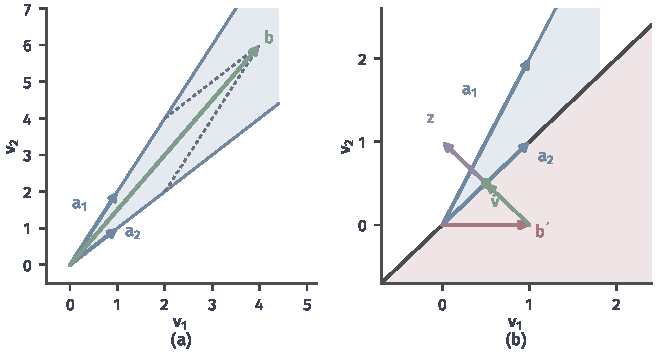
\includegraphics[width=112mm]{figures/05-optimization/01-linear-programming/matplotlib/lp-farkas-cone/figure.pdf}
 \caption{Farkas引理的几何。蓝色箭头是两列$\bm{a}_1,\bm{a}_2$，浅蓝区域是它们张成的锥。(a)~$\bm{b}=(4,6)^\top$在锥内，灰色虚线是$\bm{b}=2\bm{a}_1+2\bm{a}_2$的分解。(b)~$\bm{b}'=(1,0)^\top$在锥外，绿点$\widehat{\bm{v}}$是锥上最近的点，紫色箭头$\bm{z}=\widehat{\bm{v}}-\bm{b}'$是分离超平面（深灰线）的法向量；浅红半平面是$\bm{z}^\top\bm{v}<0$的一侧，$\bm{b}'$在其中，整个锥在另一侧。}
 \label{fig:lp-farkas-cone}
\end{BookInlineFigure}

\paragraph{强对偶}
现在回答开头的问题：只要原始问题可行且最优值有限，最好的下界就等于最优值，这个结论称为\term{强对偶}（strong duality）。

\begin{theorem}[线性规划强对偶]
 \label{thm:lp-strong-duality}
 若标准型~\eqref{eq:lp-standard}可行且最优值$p^\star$有限，则对偶问题~\eqref{eq:lp-dual}有最优解，并且
 \begin{equation}
  d^\star=p^\star.
  \label{eq:lp-strong-duality}
 \end{equation}
\end{theorem}

\begin{proof}
 只需找到$(\bm{y},\bm{s})$对偶可行，且$\bm{b}^\top\bm{y}\geq p^\star$，弱对偶就会迫使等号成立。把要求写成带非负变量的等式组，引入$r\geq0$，令$\bm{y}=\bm{y}^{+}-\bm{y}^{-}$：
 \[
  \bm{A}^\top\bm{y}^{+}-\bm{A}^\top\bm{y}^{-}+\bm{s}=\bm{c},\qquad
  \bm{b}^\top\bm{y}^{+}-\bm{b}^\top\bm{y}^{-}-r=p^\star.
 \]

 假设这个系统没有非负解。由Farkas引理，存在$\bm{z}\in\mathbb{R}^n$和$\sigma\in\mathbb{R}$，对系数矩阵的四组列分别满足
 \[
  \bm{A}\bm{z}+\sigma\bm{b}\geq\bm{0},\quad
  -\bm{A}\bm{z}-\sigma\bm{b}\geq\bm{0},\quad
  \bm{z}\geq\bm{0},\quad
  -\sigma\geq0,
 \]
 并且右端的内积为负，即$\bm{c}^\top\bm{z}+\sigma p^\star<0$。记$\tau=-\sigma\geq0$，前两式合起来得到
 \[
  \bm{A}\bm{z}=\tau\bm{b},\qquad\bm{z}\geq\bm{0},\qquad\bm{c}^\top\bm{z}<\tau p^\star.
 \]

 若$\tau>0$，则$\bm{z}/\tau$是原始可行点，目标值小于$p^\star$，矛盾。若$\tau=0$，则$\bm{A}\bm{z}=\bm{0}$，$\bm{z}\geq\bm{0}$，$\bm{c}^\top\bm{z}<0$。任取可行点$\widehat{\bm{x}}$，$\widehat{\bm{x}}+t\bm{z}$对一切$t\geq0$可行，目标趋于$-\infty$，与$p^\star$有限矛盾。

 所以系统有解，得到对偶可行的$(\bm{y},\bm{s})$和$\bm{b}^\top\bm{y}=p^\star+r\geq p^\star$。由弱对偶，$\bm{b}^\top\bm{y}\leq p^\star$，因此$\bm{b}^\top\bm{y}=p^\star$，这个$(\bm{y},\bm{s})$是对偶最优解。
\end{proof}

证明里两种情形各用了一个条件：$\tau>0$时用到$p^\star$是下确界，$\tau=0$时用到问题可行且有下界。线性规划的强对偶不需要其他条件。一般的凸问题则不然，第~\ref{chap:duality}章会在Lagrange函数的框架下说明，零间隙还需要额外的假设。

\paragraph{互补松弛与零间隙证书}
强对偶告诉我们证书一定存在，弱对偶告诉我们怎样核对它。把两者合起来，就是线性规划的最优性判别。

\begin{theorem}[零间隙证书与互补松弛]
 \label{thm:lp-optimality-certificate}
 设标准型的$\bm{x}$和$(\bm{y},\bm{s})$满足
 \begin{equation}
  \bm{A}\bm{x}=\bm{b},\quad\bm{x}\geq\bm{0},\qquad
  \bm{A}^\top\bm{y}+\bm{s}=\bm{c},\quad\bm{s}\geq\bm{0}.
  \label{eq:lp-pd-feasible}
 \end{equation}
 则下面三条等价：$\bm{x}$和$(\bm{y},\bm{s})$分别是原始、对偶最优解；$\bm{c}^\top\bm{x}=\bm{b}^\top\bm{y}$；对每个$j$，
 \begin{equation}
  x_js_j=0.
  \label{eq:lp-complementary}
 \end{equation}
\end{theorem}

\begin{proof}
 由式~\eqref{eq:lp-weak-duality}，第二条等价于$\bm{x}^\top\bm{s}=0$。$\bm{x}^\top\bm{s}$是非负数$x_js_j$之和，为零当且仅当每一项为零，这就是第三条。第二条推出第一条是弱对偶的结论。反过来若两者都最优，由强对偶知两个最优值相等，得到第二条。
\end{proof}

式~\eqref{eq:lp-complementary}称为\term{互补松弛}（complementary slackness）。它说的是，每对$(x_j,s_j)$中至少有一个为零。用价格的语言：正在生产的产品没有多余的利润，有多余的资源价格为零。第~\ref{chap:lp-interior-point}章的算法正是围绕这组方程组织的。

有了最优解的猜测，互补松弛还能反过来求出价格。车间问题中$\bm{x}^\star=(2,2,0,0)^\top$，$x_1,x_2>0$要求$s_1=s_2=0$，也就是
\[
 y_1+2y_2=-3,\qquad y_1+y_2=-2.
\]
解得$\bm{y}=(-1,-1)^\top$，再算出其余的对偶松弛：
\[
 s_3=-y_1=1,\qquad s_4=-y_2=1.
\]
$\bm{s}=(0,0,1,1)^\top\geq\bm{0}$，对偶可行，并且$\bm{b}^\top\bm{y}=-10=\bm{c}^\top\bm{x}^\star$。这一对点就是最优性的完整证书。

不是最优的顶点通不过同样的检查。取$(3,0)$，即$\bm{x}=(3,0,1,0)^\top$。$x_1,x_3>0$要求$s_1=s_3=0$，于是
\[
 y_1=0,\qquad y_2=-\frac32,\qquad s_2=-2-y_1-y_2=-\frac12<0.
\]
满足互补松弛的$\bm{y}$只有这一个，它不对偶可行，所以$(3,0)$不是最优解。

这个判别有直接的几何含义。回到平面上，顶点处的活动约束有各自的外法向量。互补松弛说的是，利润向量$\bm{p}$是活动约束法向量的非负组合。图~\ref{fig:lp-normal-cone}在两个顶点上比较：$(2,2)$处$\bm{p}=1\cdot\bm{n}_1+1\cdot\bm{n}_2$，系数正是价格$\bm{u}=(1,1)$；$(3,0)$处活动约束的法向量是$\bm{n}_2=(2,1)$和$\bm{n}_3=(0,-1)$，分解
\[
 \begin{bmatrix}3\\2\end{bmatrix}=\frac32\begin{bmatrix}2\\1\end{bmatrix}-\frac12\begin{bmatrix}0\\-1\end{bmatrix}
\]
含负系数，$\bm{p}$在锥外，负系数$-1/2$正是上面算出的$s_2$。

\begin{BookInlineFigure}
 \centering
 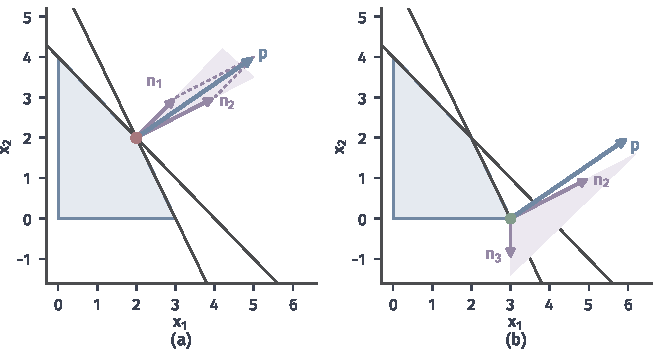
\includegraphics[width=112mm]{figures/05-optimization/01-linear-programming/matplotlib/lp-normal-cone/figure.pdf}
 \caption{互补松弛的几何。紫色箭头是顶点处活动约束的外法向量，浅紫区域是它们张成的锥，蓝色箭头是利润向量$\mathbf{p}=(3,2)$。(a)~$(2,2)$处，$\mathbf{p}$在锥内，是两个法向量的正组合（紫色虚线），该顶点最优。(b)~$(3,0)$处，$\mathbf{p}$在锥外，该顶点不是最优解。}
 \label{fig:lp-normal-cone}
\end{BookInlineFigure}

价格还有边际价值的含义。把工时从$4$增加到$5$，新的最优产量是$(1,4)$，利润$11$，恰好增加$u_1=1$。这种关系只在一定范围内成立，第~\ref{chap:simplex-method}章固定最优基时会算出这个范围。

\paragraph{三种结局的证书}
线性规划只有三种结局，每种都有可以独立核对的证据。有最优解时，证书是满足式~\eqref{eq:lp-pd-feasible}和式~\eqref{eq:lp-complementary}的一对点。不可行时，证书是满足式~\eqref{eq:lp-farkas-dual}的$\bm{z}$。无下界时，证书是一个可行点加上满足下式的方向：
\begin{equation}
 \bm{A}\bm{d}=\bm{0},\qquad\bm{d}\geq\bm{0},\qquad\bm{c}^\top\bm{d}<0.
 \label{eq:lp-unbounded-certificate}
\end{equation}

两个问题的结局也互相牵制。原始无下界时，对偶不可能有可行点，否则弱对偶会给出有限下界，所以对偶不可行。由对称性，对偶无上界时原始不可行。两者都不可行的情形确实存在，例如
\[
 \min\ -x_1-x_2\quad\text{s.t.}\quad x_1-x_2=1,\quad-x_1+x_2=1,\quad\bm{x}\geq\bm{0}.
\]
两个等式相加得到$0=2$，原始不可行；对偶约束$y_1-y_2\leq-1$和$-y_1+y_2\leq-1$相加得到$0\leq-2$，对偶也不可行。

这个例子中方向$\bm{d}=(1,1)^\top$满足式~\eqref{eq:lp-unbounded-certificate}，但没有可行的起点，它什么也说明不了。所以报告无下界时，可行点和方向缺一不可。表~\ref{tab:lp-outcomes}列出全部可能的组合。

\begin{BookInlineTable}
 \centering
 \begin{tabular}{llll}
  \toprule
  原始＼对偶 & 有最优解 & 无上界 & 不可行 \\
  \midrule
  有最优解 & 可能，且$p^\star=d^\star$ & 不可能 & 不可能 \\
  无下界 & 不可能 & 不可能 & 可能 \\
  不可行 & 不可能 & 可能 & 可能 \\
  \bottomrule
 \end{tabular}
 \caption{原始问题与对偶问题结局的组合。两个“有最优解”以外的“不可能”分别由强对偶、弱对偶和对称性得到。}
 \label{tab:lp-outcomes}
\end{BookInlineTable}

\paragraph{图中的流问题}
第~\ref{sec:lp-formulation}节的网络流实例能让对偶问题有具体的含义。关联矩阵~\eqref{eq:lp-network-data}的列是$\bm{a}_{i,j}=\bm{e}_i-\bm{e}_j$，所以$\bm{a}_{i,j}^\top\bm{y}=y_i-y_j$，对偶约束是逐弧的不等式，这里$\bm{e}_i$是第$i$个单位向量：
\begin{equation}
 s_{i,j}=c_{i,j}-(y_i-y_j)\geq0.
 \label{eq:lp-network-dual}
\end{equation}
$y_i$是节点上的数，可以读成“从节点$i$把一单位货物送到终点的费用估计”，这种量通常称为节点势。式~\eqref{eq:lp-network-dual}要求沿弧走一步，费用估计的下降不能超过这条弧的费用。对偶目标$\bm{b}^\top\bm{y}=y_1-y_4$是起点和终点的势差。

矩阵的四行线性相关，这时$\bm{y}$可以整体加一个常数而不影响任何$y_i-y_j$，所以取$y_4=0$，这相当于删去第四行。令最短路$1\to2\to3\to4$上的三条弧都取等号，得到
\[
 y_3=2,\qquad y_2=y_3+1=3,\qquad y_1=y_2+2=5.
\]
其余两条弧的对偶松弛为
\[
 s_{1,3}=5-(5-2)=2,\qquad s_{2,4}=6-(3-0)=3.
\]

路径$1\to2\to3\to4$的流量为$1$，总费用$2+1+2=5$，而$\bm{b}^\top\bm{y}=5-0=5$，两者相等。图~\ref{fig:lp-network-dual}显示了这份证书，互补松弛说的是：只有$s_{i,j}=0$的弧上才允许有流量。

\begin{BookInlineFigure}
 \centering
 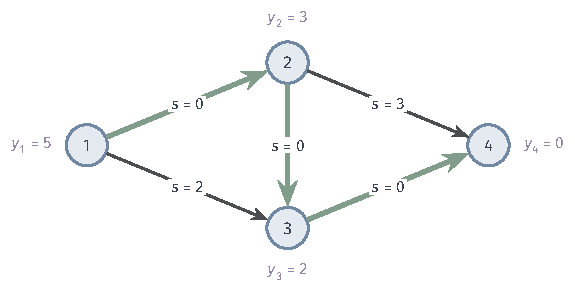
\includegraphics[width=97mm]{figures/05-optimization/01-linear-programming/tikz/lp-network-dual/figure.pdf}
 \caption{图~\ref{fig:lp-network-instance}实例的对偶证书。节点旁的紫色数字是节点势$y_i$，弧旁是对偶松弛$s_{i,j}$。绿色粗线是流量为$1$的最短路，这些弧上$s_{i,j}=0$，其余两条弧无流量。}
 \label{fig:lp-network-dual}
\end{BookInlineFigure}

这份证书正是图算法中逐弧检查的最优性条件。最短路的逐弧不等式和最小费用流的节点势都是对偶可行性，可参考\BookChapterRef{chap:shortest-paths}{卷三第3章“最短路”}；最大流最小割定理也是这种配对关系的特例，割给出流量的上界，可参考\BookChapterRef{chap:max-flow-min-cut}{卷三第5章“最大流与最小割”}。一般凸问题的对偶由第~\ref{chap:duality}章用Lagrange函数统一处理，线性规划是其中条件最宽松的情形。

\section{线性松弛}
\label{sec:lp-relaxation}

产品如果只能整批生产，变量就必须取整数。于是要问：去掉整数要求之后，连续问题的解和最优值能告诉我们整数问题的什么？回答分三层：最优值总能给出一个界；在特殊的矩阵结构下，顶点自动是整数；一般情形下，连续解还要经过专门论证的处理，才能变成原问题的可行解。

\paragraph{整数问题与它的松弛}
在标准型或不等式形式的线性规划上再要求变量取整数，就得到\term{整数线性规划}（integer linear programming）。设
\begin{equation}
 p_{\mathrm{I}}=\min\{\bm{c}^\top\bm{x}:\bm{x}\in\bm{C},\ \bm{x}\in\mathbb{Z}^n\},
 \qquad
 p_{\mathrm{R}}=\min\{\bm{c}^\top\bm{x}:\bm{x}\in\bm{C}\}.
 \label{eq:lp-relaxation-values}
\end{equation}
去掉整数要求后的问题称为原问题的\term{线性松弛}（linear relaxation）。这里的$\bm{C}$可以是任何多面体。

松弛扩大了可行集，最小化时最优值只会变小或不变。这是下面定理的全部内容，也是松弛提供的最基本的信息。

\begin{theorem}[松弛给出下界]
 \label{thm:lp-relaxation-bound}
 若整数问题可行且松弛的最优值有限，则
 \begin{equation}
  p_{\mathrm{R}}\leq p_{\mathrm{I}}.
  \label{eq:lp-relaxation-bound}
 \end{equation}
 若松弛有一个最优解是整数向量，则它也是整数问题的最优解，且等号成立。
\end{theorem}

\begin{proof}
 整数问题的可行点都在$\bm{C}$中，在较大的集合上取最小值不会更大，得到式~\eqref{eq:lp-relaxation-bound}。若松弛的最优解$\bm{x}$是整数向量，它对整数问题可行，于是
 \[
  p_{\mathrm{I}}\leq\bm{c}^\top\bm{x}=p_{\mathrm{R}}.
 \]
 再与式~\eqref{eq:lp-relaxation-bound}合并，等号成立。
\end{proof}

用一个具体的整数问题走一遍。把车间的原料增加到$7$份，利润系数改成$(3,1)$，并要求产量取整数：
\[
 \max\ 3x_1+x_2\quad\text{s.t.}\quad x_1+x_2\leq4,\quad2x_1+x_2\leq7,\quad\bm{x}\geq\bm{0},\quad\bm{x}\in\mathbb{Z}^2.
\]
松弛的四个顶点是$(0,0),(7/2,0),(3,1),(0,4)$，对应的利润依次是
\[
 0,\qquad\frac{21}{2},\qquad10,\qquad4.
\]
所以松弛的最优解是$(7/2,0)$，最优利润$21/2$。按$x_1$的取值逐个比较可行的整数点，$x_1$固定时$x_2$取最大，四种情形的利润依次是
\[
 x_1=0:\ 4,\qquad x_1=1:\ 6,\qquad x_1=2:\ 8,\qquad x_1=3:\ 10.
\]
$x_1\geq4$时原料不够，所以整数问题的最优解是$(3,1)$，利润$10$。这里是最大化，松弛给出的是上界，写成最小化$-3x_1-x_2$时，就是$p_{\mathrm{R}}=-21/2\leq-10=p_{\mathrm{I}}$。

\paragraph{舍入不是免费的}
最直接的想法是把松弛解舍入成整数。图~\ref{fig:lp-rounding}显示这个想法的问题。$(7/2,0)$向上取整得到$(4,0)$，用掉$8$份原料，不可行。向下取整得到$(3,0)$，可行，利润只有$9$，也不是最优。真正的最优解$(3,1)$在$x_2$上离松弛解差了一整个单位，它不是任何一种舍入的结果。

\begin{BookInlineFigure}
 \centering
 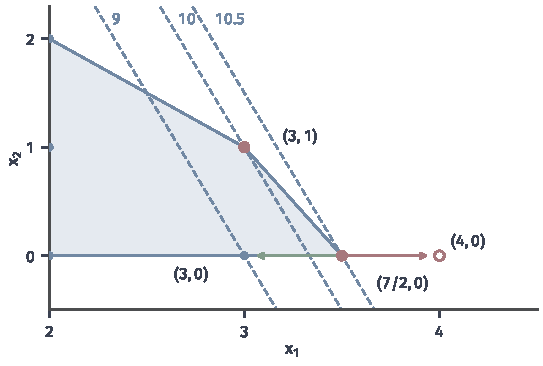
\includegraphics[width=92mm]{figures/05-optimization/01-linear-programming/matplotlib/lp-rounding/figure.pdf}
 \caption{舍入松弛解。蓝点是可行的整数点，蓝色虚线是利润$9$、$10$、$10.5$的等值线。松弛最优解$(7/2,0)$（红点，位于右下顶点）向右舍入到不可行的$(4,0)$（红色空心点），向左舍入到利润只有$9$的$(3,0)$；整数最优解是红点$(3,1)$。}
 \label{fig:lp-rounding}
\end{BookInlineFigure}

松弛最优值虽然不直接给出解，却给出了一个证明的工具。目标系数和变量都是整数时，$p_{\mathrm{I}}$也是整数，所以下界可以向上取整：
\[
 p_{\mathrm{I}}\geq\lceil p_{\mathrm{R}}\rceil=\Bigl\lceil-\frac{21}{2}\Bigr\rceil=-10.
\]
而$(3,1)$的目标值恰好是$-10$，这就证明了它是最优的，不需要枚举。一般情形下，松弛最优值和某个可行整数点的目标值夹出的区间，是对整数最优值的一个估计，这个区间的宽度取决于松弛有多紧。

$p_{\mathrm{I}}-p_{\mathrm{R}}$称为这个实例的\term{整数间隙}（integrality gap），这里是$1/2$。整数间隙衡量松弛对原问题的逼近程度，与求解松弛的算法无关。

\paragraph{整数顶点：全幺模}
既然线性规划的最优解可以在顶点取得，顶点若都是整数，整数约束就没有额外的代价。对比图~\ref{fig:lp-integer-hull}的两个多面体，它们的矩阵相同，右端不同：原料为$6$时四个顶点都是整数，原料为$7$时出现了分数顶点$(7/2,0)$。顶点是否整数，到底由什么决定？

\begin{BookInlineFigure}
 \centering
 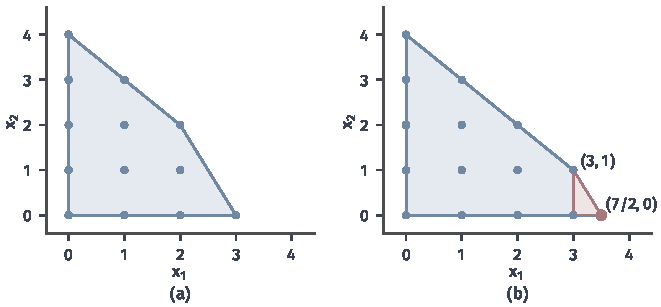
\includegraphics[width=112mm]{figures/05-optimization/01-linear-programming/matplotlib/lp-integer-hull/figure.pdf}
 \caption{相同的约束矩阵，不同的右端。蓝点是可行的整数点。(a)~原料为$6$，四个顶点都是整数。(b)~原料为$7$，右下顶点$(7/2,0)$是分数，红色小三角形是松弛比全体整数点的凸包多出的部分。}
 \label{fig:lp-integer-hull}
\end{BookInlineFigure}

答案在定义基本解的式~\eqref{eq:lp-basic-solution}里。由Cramer法则，
\[
 (\bm{x}_B)_i=\frac{\det\bm{A}_B^{(i)}}{\det\bm{A}_B},
\]
其中$\bm{A}_B^{(i)}$是把$\bm{A}_B$的第$i$列换成$\bm{b}$得到的矩阵。$\bm{A}$和$\bm{b}$都是整数时分子是整数，分数只能来自分母。如果基矩阵的行列式总是$\pm1$，顶点就一定是整数。图~\ref{fig:lp-integer-hull}(b)的分数顶点来自基$\{1,3\}$，它的行列式是$-2$，分母是$2$，而$7$是奇数；$b_2=6$时$6/2$仍是整数，分母恰好被消去。

\begin{definition}[全幺模矩阵]
 \label{def:lp-tu}
 若矩阵$\bm{A}$的每个方子矩阵的行列式都属于$\{0,1,-1\}$，就称$\bm{A}$是\term{全幺模矩阵}（totally unimodular matrix）。
\end{definition}

特别地，全幺模矩阵的元素都只能是$0,\pm1$。这个条件对所有方子矩阵提出要求，而不只是对基矩阵，这样它才能在加松弛变量、删冗余行这些改写后保持下来。

\begin{theorem}[全幺模与整数顶点]
 \label{thm:lp-tu-integral}
 设$\bm{A}$满行秩且全幺模，$\bm{b}$是整数向量。则$\bm{C}$的每个基本可行解都是整数向量。若问题可行且最优值有限，则存在整数最优解，从而
 \begin{equation}
  p_{\mathrm{I}}=p_{\mathrm{R}}.
  \label{eq:lp-tu-exact}
 \end{equation}
\end{theorem}

\begin{proof}
 任取基$B$。$\bm{A}_B$是可逆的方子矩阵，所以$\det\bm{A}_B=\pm1$。由Cramer法则，$\bm{x}_B$的每个分量都是整数行列式除以$\pm1$，是整数。第二句由定理~\ref{thm:lp-optimal-bfs}和定理~\ref{thm:lp-relaxation-bound}得到。
\end{proof}

不等式形式也可以用。若$\bm{A}$全幺模，则$[\bm{A}\ \ \bm{I}]$也全幺模：它的方子矩阵若含单位矩阵的列，这一列至多有一个非零元，按这一列展开，行列式化成$\bm{A}$的更小子矩阵的行列式，或者为零。于是不等式约束$\bm{A}\bm{x}\leq\bm{b}$，$\bm{x}\geq\bm{0}$在加了松弛变量之后满足定理的条件，变量的整数上界也可以同样处理。

定理的每个条件都起作用。$\bm{A}$全幺模但$\bm{b}$不是整数时，顶点就不是整数，例如$x_1\leq1/2$，$x_1\geq0$的顶点$1/2$。反过来，全幺模只是充分条件：车间矩阵含元素$2$，不是全幺模的，但$b_2=6$时顶点恰好都是整数。

定理说的是基本可行解，不是所有最优解。图~\ref{fig:lp-optimal-face}(b)那样有整条最优边的情形，边上的点可以不是整数，所以要得到整数解，必须取到顶点。

\paragraph{网络矩阵是全幺模的}
最重要的全幺模矩阵来自有向图。这正是图上的最短路、最大流、最小费用流可以用连续方法求整数解的原因。

\begin{theorem}[关联矩阵全幺模]
 \label{thm:lp-incidence-tu}
 设矩阵的每一列至多有一个$+1$、至多有一个$-1$，其余元素为零。有向图的关联矩阵就是这样的矩阵。这样的矩阵是全幺模的。
\end{theorem}

\begin{proof}
 对方子矩阵$\bm{D}$的阶数$k$归纳。$k=1$时元素属于$\{0,\pm1\}$。设$k>1$，$\bm{D}$的列也满足“至多一个$+1$、至多一个$-1$”，分三种情形。

 若某列全为零，$\det\bm{D}=0$。若某列恰有一个非零元，按这一列展开，$\det\bm{D}$等于$\pm$一个$k-1$阶子矩阵的行列式，由归纳假设属于$\{0,\pm1\}$。若每一列都恰有一个$+1$和一个$-1$，则所有行相加是零向量，$\det\bm{D}=0$。
\end{proof}

网络矩阵~\eqref{eq:lp-network-data}不是满行秩的，删去一行之后仍是全幺模矩阵的子矩阵，定理~\ref{thm:lp-tu-integral}可以使用。所以整数供需量、整数容量的最小费用流问题，线性规划的顶点解就是整数流，这正是第~\ref{sec:lp-duality}节实例中的最短路自动取$0$或$1$的原因。

二部图的情形也可以化成这个定理。把无向边看成两个非零元都是$+1$的列，二部图把顶点分成两侧，把一侧对应的行乘以$-1$，列就有了一个$+1$和一个$-1$，行列式只改变符号，所以二部图的关联矩阵也是全幺模的。这解释了指派问题的连续解为何能取整数，可参考\BookChapterRef{chap:bipartite-matching-assignment}{卷三第6章“二部图匹配与指派”}。

\paragraph{整数点的凸包}
全幺模解决了一类问题，一般情形还可以这样理解。有限个点$\bm{v}_1,\ldots,\bm{v}_k$的凸包是它们全部的加权平均，权重非负且和为$1$。线性目标在凸包上的最小值，等于在这些点上的最小值，因为加权平均不会比最小的项更小。

所以，若能把全体整数可行点的凸包用线性不等式写出来，整数问题就成了线性规划，图~\ref{fig:lp-integer-hull}(a)就是这种幸运的情形，松弛恰好等于这个凸包。图~\ref{fig:lp-integer-hull}(b)中松弛比凸包多了一块，多出来的部分造成了整数间隙。困难在于，一般的整数问题的凸包写不出来，不等式的条数可能随规模急剧增长。

\paragraph{一般情形：分数顶点}
图中只要出现奇圈，上面的论证就失效。考虑三个顶点的完全图（三角形），要选出尽量少的顶点，使每条边至少有一个端点被选中。这称为\term{顶点覆盖}（vertex cover）。用$x_i\in\{0,1\}$表示是否选中顶点$i$，问题是
\begin{equation}
 \min\ x_1+x_2+x_3
 \quad\text{s.t.}\quad x_1+x_2\geq1,\quad x_2+x_3\geq1,\quad x_1+x_3\geq1.
 \label{eq:lp-triangle-cover}
\end{equation}
松弛把$x_i\in\{0,1\}$放宽为$x_i\geq0$。三条约束取等号解出的点是
\[
 \bm{x}=\Bigl(\frac12,\frac12,\frac12\Bigr)^\top,\qquad\text{目标值}\ \frac32.
\]

它确实是松弛的最优解。把三条约束相加，得到$2(x_1+x_2+x_3)\geq3$，这正是取权重$(1/2,1/2,1/2)$的对偶证书，于是$p_{\mathrm{R}}=3/2$。

分数从哪里来？三条约束的系数矩阵是
\[
 \bm{E}=\begin{bmatrix}1&1&0\\0&1&1\\1&0&1\end{bmatrix},\qquad\det\bm{E}=2.
\]
行列式是$2$，所以不是全幺模矩阵，Cramer法则的分母正是$2$。三角形是奇圈，不能分成两侧，二部图的变号办法用不上。

整数问题的最优值是$2$：只选一个顶点时，对边的两端都没被选中，这条边没有被覆盖，所以至少选两个；选两个正好够。图~\ref{fig:lp-triangle-cover}对比了三种取值，这个实例的整数间隙是$2-3/2=1/2$。

\begin{BookInlineFigure}
 \centering
 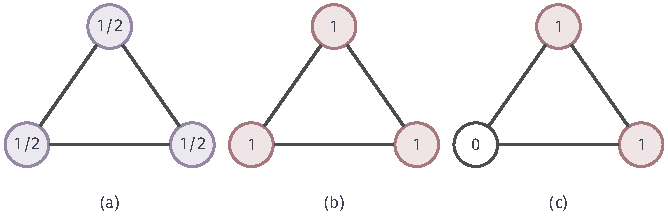
\includegraphics[width=112mm]{figures/05-optimization/01-linear-programming/tikz/lp-triangle-cover/figure.pdf}
 \caption{三角形上的顶点覆盖。圆内的数字是变量取值。(a)~松弛的最优解，三个变量都是$1/2$，目标值$3/2$。(b)~按阈值$1/2$舍入，三个变量都变成$1$，可行，目标值$3$。(c)~整数最优解之一，选两个顶点，目标值$2$。}
 \label{fig:lp-triangle-cover}
\end{BookInlineFigure}

\paragraph{从松弛解恢复可行解}
一般情形下，松弛解未必是整数，需要一个恢复步骤。恢复之后要分别回答两个问题：得到的点可行吗？目标值损失了多少？这两件事都要针对具体的约束结构来证明。前面的车间例子说明，随手舍入可能直接破坏可行性。

顶点覆盖是能够完整论证的例子。设无向图的顶点集为$V$，边集为$E$，顶点权重$w_i\geq0$。求解松弛
\[
 \min\ \sum_{i\in V}w_ix_i\quad\text{s.t.}\quad x_i+x_j\geq1\ \ (\{i,j\}\in E),\quad\bm{x}\geq\bm{0},
\]
得到最优解$\bm{x}^\star$，然后按阈值舍入：$x_i^\star\geq1/2$时取$\widehat{x}_i=1$，否则取$\widehat{x}_i=0$。

\begin{theorem}[顶点覆盖的阈值舍入]
 \label{thm:lp-cover-rounding}
 上述$\widehat{\bm{x}}$是可行的顶点覆盖，并且
 \begin{equation}
  \sum_{i\in V}w_i\widehat{x}_i\leq2\,p_{\mathrm{R}}\leq2\,p_{\mathrm{I}}.
  \label{eq:lp-cover-rounding}
 \end{equation}
\end{theorem}

\begin{proof}
 可行性：对每条边$\{i,j\}$，$x_i^\star+x_j^\star\geq1$，两个数中至少有一个不小于$1/2$，相应的$\widehat{x}$取$1$，这条边被覆盖。

 目标值：按舍入规则，每个$i$都满足$\widehat{x}_i\leq2x_i^\star$。权重非负，逐项相加，得到
 \[
  \sum_{i\in V}w_i\widehat{x}_i\leq2\sum_{i\in V}w_ix_i^\star=2p_{\mathrm{R}}.
 \]
 第二个不等号是定理~\ref{thm:lp-relaxation-bound}。
\end{proof}

三角形上这个界是$3\leq2\cdot\frac32$，等号成立，实际的最优值是$2$。系数$2$不能靠这种比较再改善。在$k$个顶点的完全图上，取单位权重，把全部边的约束相加，每个顶点出现$k-1$次，得到
\[
 (k-1)\sum_ix_i\geq\frac{k(k-1)}{2},\qquad\text{即}\qquad\sum_ix_i\geq\frac{k}{2}.
\]
全取$1/2$可以达到这个下界，松弛最优值是$k/2$。整数解至多有一个顶点不选，否则两个不选的顶点之间的边没被覆盖，所以整数最优值是$k-1$。两者之比随$k$增大趋于$2$。

这个定理的两个结论都依赖顶点覆盖的结构：可行性靠“两个数之和不小于$1$”，误差靠权重非负。换一种约束，例如前面车间的问题，同样的阈值可能得到不可行的点。所以，线性松弛本身只提供界和一个出发点，恢复原问题可行解的方法要逐类设计，并单独论证可行性和误差保证。

松弛的界不紧或者恢复的解不够好时，还可以继续加入有效的不等式来收紧松弛，或者把问题分成子问题分别求解。这类方法都要反复求解线性规划，第~\ref{chap:simplex-method}章将说明怎样在约束增加之后，利用已有的基接着求解。

\section{本章小结}
\label{sec:lp-summary}

回到章首的车间。等利润线在四边形上平移、最后停在角点，这幅图景在本章变成了三个可以计算的结论，它们的关系如图~\ref{fig:lp-summary-map}。

\begin{BookInlineFigure}
 \centering
 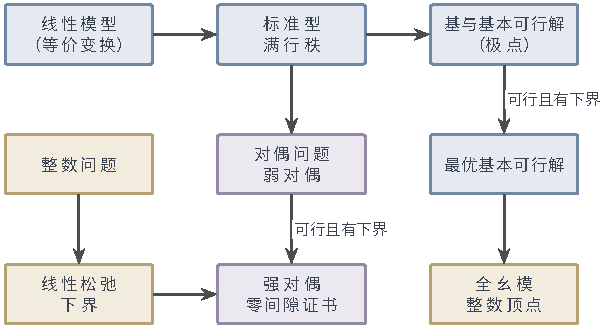
\includegraphics[width=102mm]{figures/05-optimization/01-linear-programming/tikz/lp-summary-map/figure.pdf}
 \caption{本章各部分的关系。蓝色框是原始问题的结构，紫色框是对偶与证书，黄色框是整数问题。箭头旁的文字是结论成立所需的条件。}
 \label{fig:lp-summary-map}
\end{BookInlineFigure}

第一，形式的统一。各种线性模型经过等价变换都能写成标准型，改写时松弛变量一一对应地保留可行集的形状，自由变量的分解保留最优值却可能多出角点。检查等式相容并删去冗余行之后，$\bm{A}$满行秩，基矩阵才有定义。

第二，解的位置。基本可行解就是可行集的极点，它由一个可逆的基矩阵解出；标准型只要可行且最优值有限，最优解就能在这有限个点中取得。非退化时换基对应沿边走到相邻顶点，退化时换基可能不移动，$\bm{u}\leq\bm{0}$时则得到无界可行方向。这个顶点结论依赖非负约束排除直线，含直线的多面体没有极点。

第三，解的证据。给约束配权重得到对偶问题，弱对偶说明对偶间隙等于$\bm{x}^\top\bm{s}$，因而非负，强对偶说明间隙可以精确为零。一对可行点满足互补松弛，就是最优性的完整证书，核对它只需矩阵乘法。表~\ref{tab:lp-summary}把这些结论和条件放在一起。

\begin{BookInlineTable}
 \centering
 \begin{tabular}{ll}
  \toprule
  结论 & 所需条件 \\
  \midrule
  基本可行解等于极点 & $\bm{A}$满行秩 \\
  存在最优基本可行解 & 标准型可行，最优值有限 \\
  沿边到不同的相邻顶点 & 基分量全为正，$\bm{u}$有正分量 \\
  弱对偶 & 两侧都可行 \\
  强对偶，对偶最优解存在 & 原始可行，最优值有限 \\
  松弛给出下界 & 最小化问题 \\
  顶点都是整数 & $\bm{A}$全幺模，$\bm{b}$是整数 \\
  \bottomrule
 \end{tabular}
 \caption{本章主要结论及其条件。}
 \label{tab:lp-summary}
\end{BookInlineTable}

整数问题是另一类问题。线性松弛提供一个界；全幺模配合整数右端保证顶点是整数，网络问题属于这一类；一般情形下松弛解可能是分数，恢复可行解需要针对具体结构论证可行性和误差。

本章说明了最优解在哪里、怎样核实，但没有给出高效的求解方法。第~\ref{chap:simplex-method}章沿着基本可行解换基前进，直到拿到零间隙证书。第~\ref{chap:lp-interior-point}章从可行集内部出发，保持$\bm{x}$和$\bm{s}$为正，逐步缩小互补松弛的残差。


\chapter{单纯形法}
\label{chap:simplex-method}

一家工厂用三种有限的资源生产两种产品，要定下各生产多少，使利润最大。第~\ref{chap:linear-programming}章说明，这类线性规划若有最优解，就有一个最优解落在可行域的顶点上，而且顶点可以用线性代数写成基本可行解。顶点的个数有限，却可能极多，逐个比较并不可行。\term{单纯形法}（simplex method）的做法是从一个顶点出发，每次沿一条能改善目标的边走到相邻顶点，直到手里拿到一张能证明“不必再走”的凭证。

本章用同一个工厂例子把这件事算到底。先建立一次换基怎样算、什么时候可以停；再回答第一个顶点从哪里来，遇到几条约束挤在同一个顶点时会发生什么，以及大规模问题上这些计算怎样组织。有了最优基之后，还能在资源或价格变化时复用它：对偶单纯形法从失去可行性的基接着求解，固定基的参数分析则直接读出结论成立的范围。最后一节用一族构造好的例子说明，换基的次数在最坏情形下可以随维数指数增长。

\section{换基与最优性判别}
\label{sec:simplex-basis-exchange}

手里已经有一个可行的顶点时，怎样判断它是不是最优；如果不是，下一步该走到哪里？

\paragraph{一个资源配置问题}
工厂生产两种产品，产量分别记为$x_1,x_2$，单位利润分别是$4$和$5$。原料有$8$单位，工时有$10$单位，产品二还要占用一台专用设备，设备最多加工$3$单位。两种产品对原料和工时的消耗写在下面的约束里，于是问题是
\begin{equation}
 \begin{aligned}
 \max_{x_1,x_2}\quad & 4x_1+5x_2\\
 \text{s.t.}\quad & x_1+2x_2\leq 8,\\
 & 2x_1+x_2\leq 10,\\
 & x_2\leq 3,\qquad x_1,x_2\geq 0.
 \end{aligned}
 \label{eq:simplex-resource-problem}
\end{equation}
图~\ref{fig:simplex-resource-vertices}画出它的可行域，这是一个有五个顶点的多边形。虚线是利润的等值线，沿箭头方向利润增大，最后离开多边形的那个点就是最优解。

\begin{BookInlineFigure}
 \centering
 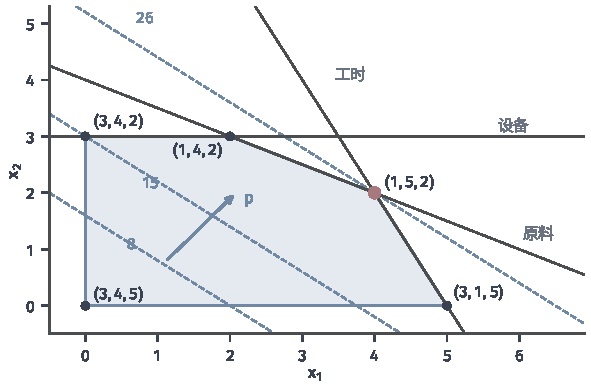
\includegraphics[width=100mm]{figures/05-optimization/01-linear-programming/matplotlib/simplex-resource-vertices/figure.pdf}
 \caption{资源配置问题~\eqref{eq:simplex-resource-problem}的可行域（浅蓝）。三条深灰线分别是原料、工时和设备约束的边界，蓝色虚线是利润$4x_1+5x_2$取$8,15,26$的等值线，箭头$\bm{p}=(4,5)$指向利润增大的方向。每个顶点旁的三元组是它对应的基，红点是最优顶点$(4,2)$。}
 \label{fig:simplex-resource-vertices}
\end{BookInlineFigure}

二维时用眼睛就能找到最优点，但变量一多就画不出来，需要把“在顶点上看哪条边更好”翻译成矩阵运算。先引入松弛变量$x_3,x_4,x_5\geq0$，分别表示没有用完的原料、工时和设备能力，并把最大化改写成最小化，得到第~\ref{chap:linear-programming}章的标准型
\begin{equation}
 \min_{\bm{x}}\ \bm{c}^\top\bm{x}\quad\text{s.t.}\quad \bm{A}\bm{x}=\bm{b},\quad \bm{x}\geq\bm{0},
 \label{eq:simplex-standard-form}
\end{equation}
其中$\bm{A}\in\mathbb{R}^{m\times n}$满行秩，第$j$列记为$\bm{a}_j=\bm{A}_{:,j}$。本例中$m=3$，$n=5$，数据是
\begin{equation}
 \bm{A}=\begin{bmatrix}1&2&1&0&0\\2&1&0&1&0\\0&1&0&0&1\end{bmatrix},\quad
 \bm{b}=\begin{bmatrix}8\\10\\3\end{bmatrix},\quad
 \bm{c}=\begin{bmatrix}-4\\-5\\0\\0\\0\end{bmatrix}.
 \label{eq:simplex-resource-data}
\end{equation}
最小化的目标值$f=\bm{c}^\top\bm{x}$是负的利润，所以下文中$f$越小，利润越大。

\paragraph{基与顶点}
第~\ref{chap:linear-programming}章已经建立了下面要用的事实。取$m$个下标组成有序元组$B$，使基矩阵$\bm{A}_B$可逆，这样的$B$称为基，其余下标组成$N$。令非基分量为零，基分量为
\[
 \bm{x}_B=\bm{A}_B^{-1}\bm{b},\qquad \bm{x}_N=\bm{0},
\]
就得到一个基本解。$\bm{x}_B\geq\bm{0}$时它是基本可行解，也就是可行域的极点；问题可行且最优值有限时，最优解可以在基本可行解中取得。所以只需在基之间搜索。下标属于$B$的变量称为\term{基变量}（basic variable），其余的称为\term{非基变量}（nonbasic variable）。

以顶点$(4,2)$为例，此时原料和工时恰好用完，即$x_3=x_4=0$，而设备还余$x_5=1$。非基变量是$x_3,x_4$，基变量是$x_1,x_5,x_2$，我们把基写成$B=(1,5,2)$。元组的顺序用来对应$\bm{x}_B$的分量，换基时新变量占据被换出变量的位置，顺序因此保持稳定。

\paragraph{主要思想：用非基变量表示一切}
站在一个顶点上，我们想知道沿每条边走会怎样。非基变量恰好提供了一组局部坐标：它们此刻都是零，让其中一个变大，就是离开顶点走上一条边。因此要把基变量和目标都写成非基变量的函数。

把$\bm{A}\bm{x}=\bm{b}$按基和非基拆开，得到$\bm{A}_B\bm{x}_B+\bm{A}_N\bm{x}_N=\bm{b}$。两边左乘$\bm{A}_B^{-1}$，每个满足等式约束的点都有
\begin{equation}
 \bm{x}_B=\bm{A}_B^{-1}\bm{b}-\bm{A}_B^{-1}\bm{A}_N\bm{x}_N.
 \label{eq:simplex-basic-form}
\end{equation}
代入目标后，整理非基变量的系数：
\[
 \bm{c}^\top\bm{x}
 =\bm{c}_B^\top\bm{x}_B+\bm{c}_N^\top\bm{x}_N
 =\bm{c}_B^\top\bm{A}_B^{-1}\bm{b}
 +\bigl(\bm{c}_N^\top-\bm{c}_B^\top\bm{A}_B^{-1}\bm{A}_N\bigr)\bm{x}_N.
\]

系数里反复出现$\bm{c}_B^\top\bm{A}_B^{-1}$，把它单独命名。记
\begin{equation}
 \bm{y}=\bm{A}_B^{-\top}\bm{c}_B,
 \qquad
 s_j=c_j-\bm{a}_j^\top\bm{y}\quad(j=1,\ldots,n),
 \label{eq:simplex-reduced-cost}
\end{equation}
其中$\bm{y}\in\mathbb{R}^m$称为这个基的对偶候选，$s_j$称为$x_j$的\term{约化成本}（reduced cost）。对基变量，$\bm{A}_B^\top\bm{y}=\bm{c}_B$正好说明$s_j=0$（$j\in B$）。于是每个满足等式约束的点都有
\begin{equation}
 \bm{c}^\top\bm{x}=\bm{b}^\top\bm{y}+\sum_{j\in N}s_jx_j.
 \label{eq:simplex-objective-form}
\end{equation}

这个式子是本章的出发点。第一项是当前顶点的目标值，第二项说明：让非基变量$x_j$从零增加一个单位，目标改变$s_j$。可以这样理解这些量：$y_i$是这个基给第$i$种资源定的内部单价，$\bm{a}_j^\top\bm{y}$是生产一单位$x_j$所耗资源按内部单价折算的总价，$s_j$是$x_j$的真实成本减去这个折算价。$s_j<0$表示真实成本比折算价低，做这件事划算。

这组记号和第~\ref{chap:linear-programming}章的对偶是同一套。对偶问题要求$\bm{A}^\top\bm{y}+\bm{s}=\bm{c}$且$\bm{s}\geq\bm{0}$，而式~\eqref{eq:simplex-reduced-cost}总满足前一半，只差$\bm{s}\geq\bm{0}$。“候选”二字指的就是这一点：等式已经成立，符号条件还要检查。

\begin{theorem}[最优性判别]
 \label{thm:simplex-optimality}
 设$B$是可行基，基本可行解为$\bar{\bm{x}}$，$\bm{y},\bm{s}$由式~\eqref{eq:simplex-reduced-cost}给出。若
 \begin{equation}
  s_j\geq 0\quad\text{对所有 }j\in N\text{ 成立},
  \label{eq:simplex-optimality-condition}
 \end{equation}
 则$\bar{\bm{x}}$是标准型~\eqref{eq:simplex-standard-form}的全局最优解，$(\bm{y},\bm{s})$是对偶最优解，两者目标值相等。
\end{theorem}

\begin{proof}
 任取可行点$\bm{x}$。它满足$\bm{A}\bm{x}=\bm{b}$，所以式~\eqref{eq:simplex-objective-form}对它成立。又因$\bm{x}_N\geq\bm{0}$且$s_j\geq0$，右端第二项非负，于是
 \[
  \bm{c}^\top\bm{x}\geq\bm{b}^\top\bm{y}.
 \]
 另一方面$\bar{\bm{x}}_N=\bm{0}$，式~\eqref{eq:simplex-objective-form}给出$\bm{c}^\top\bar{\bm{x}}=\bm{b}^\top\bm{y}$。所以$\bar{\bm{x}}$的目标值不大于任何可行点的目标值。条件~\eqref{eq:simplex-optimality-condition}连同基变量的$s_j=0$说明$(\bm{y},\bm{s})$对偶可行，它的对偶目标$\bm{b}^\top\bm{y}$等于原始目标，由弱对偶知它是对偶最优解。
\end{proof}

判别只看当前顶点的约化成本，结论却是全局的，原因在于式~\eqref{eq:simplex-objective-form}对所有满足等式的点都成立，不是局部近似。约化成本全部非负，就等于对偶可行，$\bm{y}$就是第~\ref{chap:linear-programming}章说的下界证书。

定理的方向只有一个：非负是最优的充分条件。某个$s_j<0$时，当前顶点是否一定不是最优，要看沿这条边能否真的走出去，这正是下面要讨论的。

\paragraph{主要思想：沿一条边走到下一个顶点}
设$s_q<0$，$q\in N$，我们让$x_q$增大，其余非基变量保持为零。记增大的幅度为$\alpha\geq0$，由式~\eqref{eq:simplex-basic-form}，基变量随之按下式变化：
\begin{equation}
 \bm{x}_B(\alpha)=\bar{\bm{x}}_B-\alpha\bm{u},\qquad \bm{u}=\bm{A}_B^{-1}\bm{a}_q.
 \label{eq:simplex-direction}
\end{equation}
$\bm{u}$的含义很具体：$u_i$是$x_q$每增加一单位时，位于第$i$个位置的基变量要减少的量。用整个向量来写，移动方向$\bm{d}\in\mathbb{R}^n$满足$d_q=1$，$\bm{d}_B=-\bm{u}$，其余分量为零。

沿这个方向走，等式约束不被破坏，目标按$s_q$下降。两件事都可以直接验算：
\[
 \bm{A}\bm{d}=\bm{a}_q-\bm{A}_B\bm{u}=\bm{0},
 \qquad
 \bm{c}^\top\bm{d}=c_q-\bm{c}_B^\top\bm{A}_B^{-1}\bm{a}_q=s_q.
\]

图~\ref{fig:simplex-edge-rates}在顶点$(2,3)$上画出了这两种可能。这个顶点的基是$(1,4,2)$，$x_3,x_5$非基。让$x_3$增大，点沿设备约束的边向左移动，目标以速率$s_3=4$变差；让$x_5$增大，点沿原料约束的边向右下移动，目标以速率$s_5=-3$变好。

\begin{BookInlineFigure}
 \centering
 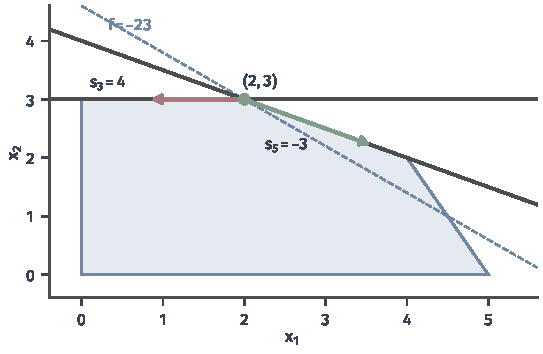
\includegraphics[width=92mm]{figures/05-optimization/01-linear-programming/matplotlib/simplex-edge-rates/figure.pdf}
 \caption{顶点$(2,3)$处的两条边。深灰粗线是在此活动的设备和原料约束，蓝色虚线是过该点的等值线$f=-23$。红色箭头是$x_3$增大的方向，走上去$f$每单位增加$4$；绿色箭头是$x_5$增大的方向，走上去$f$每单位减少$3$，它越过等值线进入利润更高的一侧。}
 \label{fig:simplex-edge-rates}
\end{BookInlineFigure}

能走多远由基变量的非负性决定。$u_i\leq0$的基变量不会减小，不构成限制；$u_i>0$的基变量在$\alpha=\bar{x}_{B(i)}/u_i$时降到零，其中$B(i)$是基中第$i$个下标。最先降到零的那个变量决定步长：
\begin{equation}
 \alpha^\star=\min_{i:\,u_i>0}\frac{\bar{x}_{B(i)}}{u_i}.
 \label{eq:simplex-ratio-test}
\end{equation}
这称为\term{比值检验}（ratio test）。像预算线一样，每种资源各自算出“还够做多少”，能做的量由最紧的那一种决定。图~\ref{fig:simplex-ratio-test}把基变量画成$\alpha$的直线，第一条碰到零的直线给出步长。

\begin{BookInlineFigure}
 \centering
 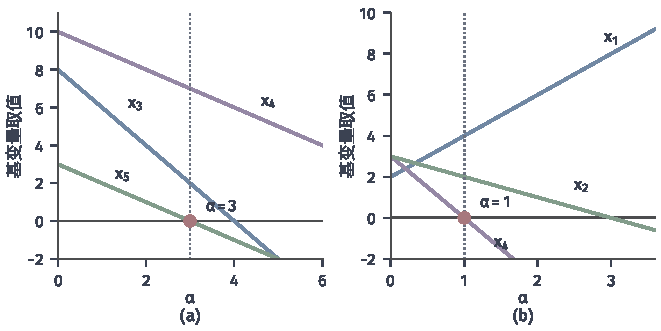
\includegraphics[width=112mm]{figures/05-optimization/01-linear-programming/matplotlib/simplex-ratio-test/figure.pdf}
 \caption{比值检验的两个实例，三条直线是基变量随步长$\alpha$的变化，红点是最先降到零的位置。(a)~入基变量$x_2$，基$(3,4,5)$，$x_5$先到零，$\alpha^\star=3$。(b)~入基变量$x_5$，基$(1,4,2)$，$x_1$随$\alpha$增大而增大，不起限制作用，$x_4$先到零，$\alpha^\star=1$。}
 \label{fig:simplex-ratio-test}
\end{BookInlineFigure}

设最小值在位置$r$取到，$p=B(r)$。走到$\alpha^\star$后$x_p=0$，$x_q=\alpha^\star$，于是把$p$从基中换出、$q$换入。$x_q$称为\term{入基变量}（entering variable），$x_p$称为\term{出基变量}（leaving variable），这一次替换称为\term{换基}（pivot）。下面的引理保证替换后仍是一个可行基。

\begin{lemma}[换基的合法性]
 \label{lem:simplex-pivot}
 设$s_q<0$，$\bm{u}$由式~\eqref{eq:simplex-direction}给出且$\bm{u}$至少有一个正分量，$r$在式~\eqref{eq:simplex-ratio-test}中取到最小值。把$B$的第$r$个下标换成$q$，得到的$B'$仍是基，$\bar{\bm{x}}+\alpha^\star\bm{d}$是它的基本可行解，目标值为
 \begin{equation}
  \bm{c}^\top\bar{\bm{x}}+\alpha^\star s_q.
  \label{eq:simplex-objective-update}
 \end{equation}
\end{lemma}

\begin{proof}
 先证$\bm{A}_{B'}$可逆。由$\bm{A}_B\bm{u}=\bm{a}_q$，有$\bm{a}_q=\sum_iu_i\bm{a}_{B(i)}$，其中$\bm{a}_{B(r)}$的系数$u_r>0$。若$\bm{A}_{B'}$的列线性相关，由于其余$m-1$列线性无关，$\bm{a}_q$就能只用这$m-1$列表示，这与$\bm{a}_q$在基$\bm{A}_B$下表示的唯一性及$u_r\neq0$矛盾。

 再看新点。由$\bm{A}\bm{d}=\bm{0}$，等式约束保持成立。$\alpha^\star$的取法使所有基变量非负，$x_q=\alpha^\star\geq0$。新点在位置$p$和$N\setminus\{q\}$上的分量都是零，也就是$B'$之外的分量都是零，所以它是$B'$的基本可行解。目标值由$\bm{c}^\top\bm{d}=s_q$得到。
\end{proof}

$\alpha^\star>0$时，目标严格下降，点从一个顶点沿边走到了相邻顶点。这就是单纯形法的全部几何内容。

\needspace{6\baselineskip}
\paragraph{变量}
下面用工厂的例子走完整个过程。计算中出现的量及其形状如下。
\begin{itemize}
 \item $B^{(t)}$：第$t$轮的基，含$m$个下标的有序元组；$N^{(t)}$是其余$n-m$个下标。
 \item $\bm{x}_B^{(t)}\in\mathbb{R}^m$：基变量的取值，非基变量都是零。
 \item $\bm{y}^{(t)}\in\mathbb{R}^m$：对偶候选。
 \item $s_j^{(t)}$：非基变量的约化成本。
 \item $q^{(t)}$：入基下标；$\bm{u}^{(t)}\in\mathbb{R}^m$：入基列在当前基下的表示。
 \item $\alpha^{(t)}\geq0$：步长；$r^{(t)}$：出基位置，$p^{(t)}=B^{(t)}(r^{(t)})$是出基下标。
\end{itemize}

\paragraph{初始化}
需要一个可行基$B^{(0)}$。当$\bm{b}\geq\bm{0}$且每个约束都带松弛变量时，取全部松弛变量为基即可，此时$\bm{A}_B=\bm{I}$。其他情形在第~\ref{sec:simplex-initial-basis}节处理。例中
\[
 B^{(0)}=(3,4,5),\qquad \bm{A}_{B^{(0)}}=\bm{I},\qquad \bm{x}_B^{(0)}=\begin{bmatrix}8\\10\\3\end{bmatrix}.
\]
对应顶点$(0,0)$，什么都不生产，$f=0$。

\needspace{6\baselineskip}
\paragraph{每轮更新}
第$t$轮依次做下面几步。步骤后的“例中”是第$0$轮的数据，其余各轮随后列出。
\begin{enumerate}

 \item 计算对偶候选。由式~\eqref{eq:simplex-reduced-cost}，
 \[
  \bm{y}^{(t)}=\bigl(\bm{A}_{B^{(t)}}\bigr)^{-\top}\bm{c}_{B^{(t)}}.
 \]
 例中$\bm{c}_B=\bm{0}$，所以
 \[
  \bm{y}^{(0)}=(0,0,0)^\top.
 \]

 \item 定价，即对每个非基下标计算约化成本$s_j^{(t)}=c_j-\bm{a}_j^\top\bm{y}^{(t)}$。例中
 \[
  s_1^{(0)}=-4,\qquad s_2^{(0)}=-5.
 \]

 \item 判别。若所有$s_j^{(t)}\geq0$，停止，当前解最优。否则选一个$s_q^{(t)}<0$的下标$q=q^{(t)}$入基。本节取约化成本最负的下标，称为\term{Dantzig规则}（Dantzig's rule），并列时取下标最小者。例中$s_2$最负，所以
 \[
  q^{(0)}=2.
 \]

 \item 计算入基列的表示。由式~\eqref{eq:simplex-direction}，
 \[
  \bm{u}^{(t)}=\bigl(\bm{A}_{B^{(t)}}\bigr)^{-1}\bm{a}_q.
 \]
 若$\bm{u}^{(t)}\leq\bm{0}$，停止，问题无界。例中
 \[
  \bm{u}^{(0)}=\bm{a}_2=(2,1,1)^\top.
 \]

 \item 比值检验。由式~\eqref{eq:simplex-ratio-test}求$\alpha^{(t)}$和出基位置$r^{(t)}$，并列时本节取下标最小的基变量。例中三个比值是
 \[
  \frac{x_3}{u_1}=\frac{8}{2}=4,\qquad
  \frac{x_4}{u_2}=\frac{10}{1}=10,\qquad
  \frac{x_5}{u_3}=\frac{3}{1}=3,
 \]
 所以
 \[
  \alpha^{(0)}=3,\qquad r^{(0)}=3,\qquad p^{(0)}=5.
 \]

 \item 更新基和基变量。除第$r$个位置外，
 \begin{equation}
  \bm{x}_B^{(t+1)}=\bm{x}_B^{(t)}-\alpha^{(t)}\bm{u}^{(t)},
  \label{eq:simplex-primal-update}
 \end{equation}
 第$r$个位置改放$x_q=\alpha^{(t)}$，并把$B^{(t)}$的第$r$个下标换成$q$。例中
 \[
  B^{(1)}=(3,4,2),\qquad \bm{x}_B^{(1)}=\begin{bmatrix}8-3\cdot2\\10-3\cdot1\\3\end{bmatrix}=\begin{bmatrix}2\\7\\3\end{bmatrix}.
 \]
 目标值由式~\eqref{eq:simplex-objective-update}变为$0+3\cdot(-5)=-15$，点走到$(0,3)$。
\end{enumerate}

例中第$1$轮的基矩阵是
\[
 \bm{A}_{B^{(1)}}=\begin{bmatrix}1&0&2\\0&1&1\\0&0&1\end{bmatrix}.
\]
解$\bm{A}_B^\top\bm{y}=\bm{c}_B$，其中$\bm{c}_B=(0,0,-5)^\top$，再计算两个非基变量的约化成本：
\[
 \bm{y}^{(1)}=(0,0,-5)^\top,\qquad s_1^{(1)}=-4,\qquad s_5^{(1)}=5.
\]
只有$s_1<0$，所以$x_1$入基。它的表示和两个有效比值为
\[
 \bm{u}^{(1)}=(1,2,0)^\top,\qquad
 \frac{x_3}{u_1}=\frac{2}{1}=2,\qquad
 \frac{x_4}{u_2}=\frac{7}{2}.
\]
第三个分量$u_3=0$，产品一不占专用设备，$x_2$不受影响。于是$\alpha^{(1)}=2$，$x_3$出基，更新后
\[
 B^{(2)}=(1,4,2),\qquad \bm{x}_B^{(2)}=\begin{bmatrix}2\\7-2\cdot2\\3\end{bmatrix}=\begin{bmatrix}2\\3\\3\end{bmatrix}.
\]
目标值变为$-15+2\cdot(-4)=-23$，点走到$(2,3)$。

例中第$2$轮的基矩阵和对偶候选是
\[
 \bm{A}_{B^{(2)}}=\begin{bmatrix}1&0&2\\2&1&1\\0&0&1\end{bmatrix},\qquad
 \bm{c}_B=\begin{bmatrix}-4\\0\\-5\end{bmatrix},\qquad
 \bm{y}^{(2)}=\begin{bmatrix}-4\\0\\3\end{bmatrix}.
\]
非基变量$x_3,x_5$的约化成本为
\[
 s_3^{(2)}=0-(-4)=4,\qquad s_5^{(2)}=0-3=-3.
\]
这里出现了一个值得留意的现象：$x_5$是设备的余量，让它入基意味着故意不用满设备。$s_5<0$说明把设备让出一些，腾出的原料拿去做产品一更赚钱。$x_5$入基，表示向量和比值为
\[
 \bm{u}^{(2)}=(-2,3,1)^\top,\qquad
 \frac{x_4}{u_2}=\frac{3}{3}=1,\qquad
 \frac{x_2}{u_3}=\frac{3}{1}=3.
\]
$u_1=-2<0$表示$x_1$会增大，不参与比较。于是$\alpha^{(2)}=1$，$x_4$出基，按式~\eqref{eq:simplex-primal-update}更新：
\[
 B^{(3)}=(1,5,2),\qquad
 \bm{x}_B^{(3)}=\begin{bmatrix}2+2\\1\\3-1\end{bmatrix}=\begin{bmatrix}4\\1\\2\end{bmatrix}.
\]
目标值变为$-23+1\cdot(-3)=-26$，点走到$(4,2)$。

例中第$3$轮的基矩阵和对偶候选是
\[
 \bm{A}_{B^{(3)}}=\begin{bmatrix}1&0&2\\2&0&1\\0&1&1\end{bmatrix},\qquad
 \bm{c}_B=\begin{bmatrix}-4\\0\\-5\end{bmatrix},\qquad
 \bm{y}^{(3)}=\begin{bmatrix}-2\\-1\\0\end{bmatrix}.
\]
非基变量$x_3,x_4$的约化成本为
\[
 s_3^{(3)}=0-(-2)=2,\qquad s_4^{(3)}=0-(-1)=1.
\]
两者都非负，算法停止。表~\ref{tab:simplex-resource-rounds}汇总了四轮的数据。

\begin{BookInlineTable}
 \centering
 \begin{tabular}{cccccc}
  \toprule
  $t$ & $B^{(t)}$ & $(x_1,x_2)$ & $f$ & $\bm{y}^{(t)}$ & 入基／出基\\
  \midrule
  $0$ & $(3,4,5)$ & $(0,0)$ & $0$ & $(0,0,0)$ & $x_2$／$x_5$\\
  $1$ & $(3,4,2)$ & $(0,3)$ & $-15$ & $(0,0,-5)$ & $x_1$／$x_3$\\
  $2$ & $(1,4,2)$ & $(2,3)$ & $-23$ & $(-4,0,3)$ & $x_5$／$x_4$\\
  $3$ & $(1,5,2)$ & $(4,2)$ & $-26$ & $(-2,-1,0)$ & 停止\\
  \bottomrule
 \end{tabular}
 \caption{资源配置问题在Dantzig规则下的各轮数据。}
 \label{tab:simplex-resource-rounds}
\end{BookInlineTable}

\paragraph{最终得到}
算法结束时得到最优基$B^\star=(1,5,2)$和最优解
\begin{equation}
 \bm{x}^\star=(4,2,0,0,1)^\top,\qquad p^\star=-26,
 \label{eq:simplex-resource-solution}
\end{equation}
即产品一做$4$、产品二做$2$，利润$26$，原料和工时用完，设备余$1$。同时得到对偶最优解
\begin{equation}
 \bm{y}^\star=(-2,-1,0)^\top,\qquad \bm{s}^\star=(0,0,2,1,0)^\top.
 \label{eq:simplex-resource-dual}
\end{equation}
证书可以当场核对：一方面$\bm{b}^\top\bm{y}^\star=-16-10=-26=p^\star$，另一方面$(\bm{x}^\star)^\top\bm{s}^\star=0$，互补松弛成立。

几何上，最优性说的是目标方向落在活动约束法向量张成的锥里。把最大化写回去，利润向量恰好是原料和工时两个法向量的非负组合：
\[
 \begin{bmatrix}4\\5\end{bmatrix}=2\begin{bmatrix}1\\2\end{bmatrix}+1\begin{bmatrix}2\\1\end{bmatrix}.
\]
图~\ref{fig:simplex-optimal-cone}画的就是这个分解，组合系数$2,1$正是$-\bm{y}^\star$的前两个分量。

\begin{BookInlineFigure}
 \centering
 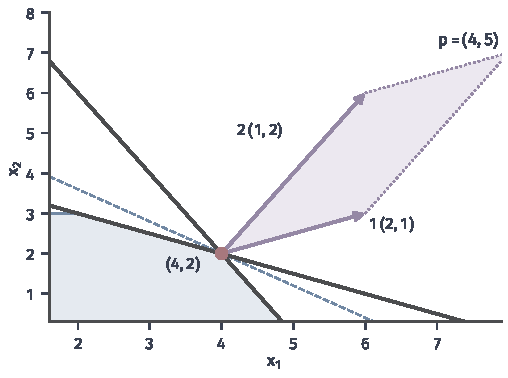
\includegraphics[width=86mm]{figures/05-optimization/01-linear-programming/matplotlib/simplex-optimal-cone/figure.pdf}
 \caption{最优顶点$(4,2)$处的对偶证书。深灰粗线是两条活动约束，紫色箭头是它们的法向量按系数$2$和$1$缩放后的结果，蓝色箭头是利润向量$\bm{p}$，它是紫色平行四边形的对角线，因此落在两个法向量张成的锥内。蓝色虚线是过该点的等值线。}
 \label{fig:simplex-optimal-cone}
\end{BookInlineFigure}

\paragraph{换基规则影响路径，不影响结论}
Dantzig规则只看单位变化率，不看能走多远。图~\ref{fig:simplex-vertex-paths}对比了同一问题上的两条路径：Dantzig规则先选利润系数大的$x_2$，走了三步；若总选下标最小的负约化成本，则先选$x_1$，经$(5,0)$两步到达。两条路径终点相同，因为最优性判别不依赖路径。这个例子不能说明后一种规则更好，它只说明步数取决于规则与问题的搭配。

\begin{BookInlineFigure}
 \centering
 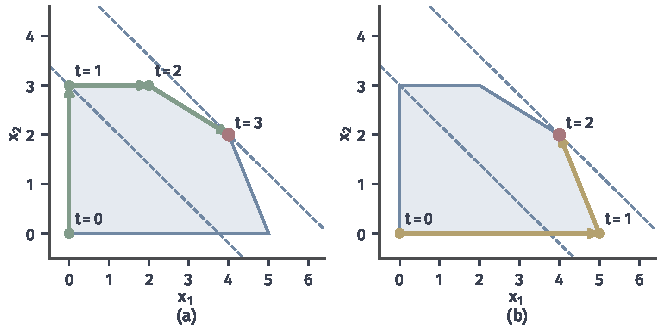
\includegraphics[width=112mm]{figures/05-optimization/01-linear-programming/matplotlib/simplex-vertex-paths/figure.pdf}
 \caption{同一问题上的两条换基路径，蓝色虚线是利润$15$和$26$的等值线，红点是最优解。(a)~Dantzig规则（绿色），经$(0,3)$和$(2,3)$共三次换基。(b)~总选下标最小的负约化成本（黄色），经$(5,0)$共两次换基。}
 \label{fig:simplex-vertex-paths}
\end{BookInlineFigure}

\paragraph{没有出基变量：无界证书}
比值检验可能找不到任何限制。此时$\bm{u}\leq\bm{0}$，对一切$\alpha\geq0$，$\bar{\bm{x}}+\alpha\bm{d}$都可行，目标按$\alpha s_q$趋于$-\infty$。这个$\bar{\bm{x}}$和$\bm{d}$合在一起就是问题无下界的证据：
\begin{equation}
 \bm{A}\bm{d}=\bm{0},\qquad \bm{d}\geq\bm{0},\qquad \bm{c}^\top\bm{d}=s_q<0.
 \label{eq:simplex-unbounded-certificate}
\end{equation}

\begin{example}[无界问题]
 \label{ex:simplex-unbounded}
 考虑最大化$x_1+x_2$，约束为$x_1-x_2\leq2$，$-x_1+x_2\leq1$，$x_1,x_2\geq0$。加松弛变量$x_3,x_4$，从$B=(3,4)$出发，约化成本是$s_1=s_2=-1$，取$x_1$入基。比值检验给出$x_3$出基，$\alpha=2$，点到达$(2,0)$。

 第二轮$B=(1,4)$，对偶候选和约化成本为
 \[
  \bm{y}=(-1,0)^\top,\qquad s_2=-2,\qquad s_3=1.
 \]
 $x_2$入基，它的表示是
 \[
  \bm{u}=(-1,0)^\top\leq\bm{0}.
 \]
 没有基变量会减小，比值检验无从进行。按式~\eqref{eq:simplex-unbounded-certificate}得到无界方向$\bm{d}=(1,1,0,0)^\top$，沿它每走一单位，目标减少$2$。
\end{example}

图~\ref{fig:simplex-unbounded}中可行域是一条向右上方延伸的带子，红色射线在带子里一直走不出去，而利润不断增大。

\begin{BookInlineFigure}
 \centering
 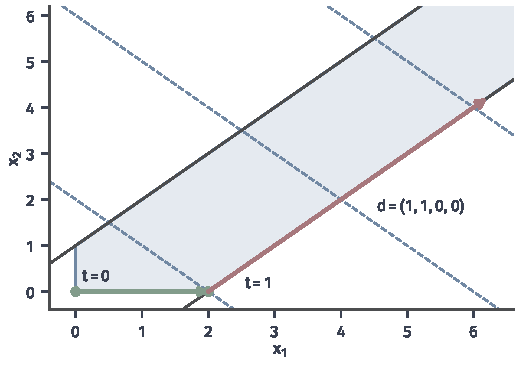
\includegraphics[width=88mm]{figures/05-optimization/01-linear-programming/matplotlib/simplex-unbounded/figure.pdf}
 \caption{例~\ref{ex:simplex-unbounded}的无界可行域（浅蓝，向右上方无限延伸）。绿色是一次换基，从$(0,0)$到$(2,0)$；红色射线是无界方向$\bm{d}$，蓝色虚线是利润$2,6,10$的等值线，射线不断穿过利润更高的等值线。}
 \label{fig:simplex-unbounded}
\end{BookInlineFigure}

\paragraph{走不动的换基}
还有一种情形需要先记下来。若某个基变量已经是零，且它对应的$u_i>0$，式~\eqref{eq:simplex-ratio-test}给出$\alpha^\star=0$。这时基换了，点没动，目标也没变，这样的基是退化基。所以$s_q<0$只说明这条边的方向改善目标，并不保证真能走出去，$\alpha^\star=0$时当前点可能已经最优。第~\ref{sec:simplex-degeneracy}节专门处理这种情形。

没有退化时，算法的终止性可以直接得出。

\begin{theorem}[非退化时的有限终止]
 \label{thm:simplex-finite-nondegenerate}
 设算法访问的每个基都非退化，则从任一可行基出发，单纯形法经过有限次换基后，或得到满足式~\eqref{eq:simplex-optimality-condition}的最优基，或得到满足式~\eqref{eq:simplex-unbounded-certificate}的无界方向。
\end{theorem}

\begin{proof}
 非退化时$\bar{\bm{x}}_B>\bm{0}$，比值检验给出$\alpha^\star>0$，由式~\eqref{eq:simplex-objective-update}，目标严格下降，所以任何基都不会重复访问。基的个数不超过从$n$个下标中选$m$个的组合数，是有限的，因此换基只能进行有限次。算法每轮要么换基，要么在两种停止条件之一下结束，由此得到结论。
\end{proof}

\section{初始可行基}
\label{sec:simplex-initial-basis}

上一节的算法要从一个可行基出发，而工厂例子里松弛变量恰好提供了一个。本节解决没有现成可行基时怎么办。

给工厂加一个合同要求：两种产品合计至少交付$2$单位，即$x_1+x_2\geq2$。这个不等式要减去一个非负的剩余变量$x_6$才能化成等式，标准型的第四行是
\begin{equation}
 x_1+x_2-x_6=2.
 \label{eq:simplex-order-row}
\end{equation}
若仍取松弛变量和剩余变量组成基，第四行给出$x_6=-2<0$，不可行。这对应图~\ref{fig:simplex-two-phase-path}中的原点：什么都不生产，合同就违约了，原点已不在可行域内。等式约束的情形更直接，它没有松弛变量可用。

\paragraph{人工变量}
解决办法是暂时允许约束被违反，并给违反量记账。把各行乘以适当的符号使$\bm{b}\geq\bm{0}$，对缺少现成基列的行，引入非负的\term{人工变量}（artificial variable）$\bm{v}$，得到扩大的约束
\begin{equation}
 \bm{A}\bm{x}+\bm{v}=\bm{b},\qquad \bm{x}\geq\bm{0},\quad \bm{v}\geq\bm{0}.
 \label{eq:simplex-artificial-system}
\end{equation}
为叙述简单，这里写成每行都加人工变量；已有松弛变量可作基列的行不必加，例中只有第四行需要。

这个系统立刻有可行基：$\bm{x}=\bm{0}$，$\bm{v}=\bm{b}$。但要分清，它是扩大问题的可行基，不是原问题的：只要某个$v_i>0$，对应的原约束就没有被满足。$\bm{v}$像一笔临时垫付的账，只有全部还清，得到的点才是原问题的可行点。

例中把人工变量记作$x_7$，扩大后的约束有四行七列：
\[
 \begin{bmatrix}
 1&2&1&0&0&0&0\\
 2&1&0&1&0&0&0\\
 0&1&0&0&1&0&0\\
 1&1&0&0&0&-1&1
 \end{bmatrix}\bm{x}
 =\begin{bmatrix}8\\10\\3\\2\end{bmatrix}.
\]
起始基$(3,4,5,7)$的基矩阵是单位矩阵，$x_7=2$就是合同的缺口。两阶段法和大M法用两种方式把这笔账还清。

\subsection{两阶段法}
\label{sec:simplex-two-phase}

\paragraph{主要思想}
\term{两阶段法}（two-phase method）把“还清账”和“优化目标”分开。第一阶段暂时不管原目标，只最小化人工变量之和：
\begin{equation}
 \min_{\bm{x},\bm{v}}\ \phi=\bm{1}^\top\bm{v}
 \quad\text{s.t.}\quad
 \bm{A}\bm{x}+\bm{v}=\bm{b},\quad\bm{x}\geq\bm{0},\quad\bm{v}\geq\bm{0}.
 \label{eq:simplex-phase-one}
\end{equation}
这个问题有现成的可行基，目标又以$0$为下界，所以单纯形法不会遇到无界，一定有最优值$\phi^\star\geq0$。它回答了可行性问题。

\begin{theorem}[第一阶段的结论]
 \label{thm:simplex-phase-one}
 原问题$\bm{A}\bm{x}=\bm{b}$，$\bm{x}\geq\bm{0}$可行，当且仅当问题~\eqref{eq:simplex-phase-one}的最优值$\phi^\star=0$。若$\phi^\star>0$，设$\bm{y}$是第一阶段最优基的对偶候选，则
 \begin{equation}
  \bm{A}^\top\bm{y}\leq\bm{0},\qquad \bm{b}^\top\bm{y}=\phi^\star>0,
  \label{eq:simplex-farkas-certificate}
 \end{equation}
 这个$\bm{y}$就是原问题不可行的证书。
\end{theorem}

\begin{proof}
 若原问题有可行点$\bm{x}$，则$(\bm{x},\bm{0})$对问题~\eqref{eq:simplex-phase-one}可行，目标为零，又因$\phi\geq0$，所以$\phi^\star=0$。反过来，$\phi^\star=0$时最优解满足$\bm{v}=\bm{0}$，它的$\bm{x}$部分满足$\bm{A}\bm{x}=\bm{b}$，$\bm{x}\geq\bm{0}$。

 设$\phi^\star>0$。第一阶段的目标系数在$\bm{x}$上是零，于是最优性条件$s_j=0-\bm{a}_j^\top\bm{y}\geq0$说明$\bm{A}^\top\bm{y}\leq\bm{0}$。由定理~\ref{thm:simplex-optimality}，两边目标值相等，即$\bm{b}^\top\bm{y}=\phi^\star$。若存在$\bm{x}\geq\bm{0}$满足$\bm{A}\bm{x}=\bm{b}$，就有
 \[
  0<\bm{b}^\top\bm{y}=\bm{x}^\top\bm{A}^\top\bm{y}\leq0,
 \]
 矛盾，这说明$\bm{y}$确实证明了不可行。
\end{proof}

\paragraph{变量}
第一阶段沿用第~\ref{sec:simplex-basis-exchange}节的全部变量，只是下标范围包括人工变量，目标向量换成在$\bm{x}$上为零、在$\bm{v}$上为一的$\bm{g}$。第二阶段回到原来的$\bm{c}$，并去掉人工变量对应的列。

\paragraph{初始化}
第一阶段从人工变量和可用的松弛变量组成的基出发。例中
\[
 B^{(0)}=(3,4,5,7),\qquad \bm{x}_B^{(0)}=(8,10,3,2)^\top,\qquad \phi=2.
\]

\needspace{6\baselineskip}
\paragraph{每轮更新}
两个阶段的每轮计算都与第~\ref{sec:simplex-basis-exchange}节相同，区别只在目标向量和两阶段之间的衔接。
\begin{enumerate}
 \item 第一阶段按$\bm{g}$运行单纯形法，直到约化成本全部非负。例中第$0$轮的对偶候选和约化成本为
 \[
  \bm{y}^{(0)}=(0,0,0,1)^\top,\qquad s_1=-1,\quad s_2=-1,\quad s_6=1.
 \]
 $s_1,s_2$并列最负，取下标小的$x_1$入基。它的表示和比值为
 \[
  \bm{u}^{(0)}=(1,2,0,1)^\top,\qquad
  \frac{8}{1}=8,\quad \frac{10}{2}=5,\quad \frac{2}{1}=2.
 \]
 于是$\alpha^{(0)}=2$，$x_7$出基，更新后
 \[
  B^{(1)}=(3,4,5,1),\qquad \bm{x}_B^{(1)}=(6,6,3,2)^\top,\qquad\phi=0.
 \]
 第$1$轮人工变量已经出基，$\bm{y}^{(1)}=\bm{0}$，所有$s_j\geq0$，第一阶段结束，得到$\phi^\star=0$和原问题的顶点$(2,0)$。
 \item 判断$\phi^\star$。若$\phi^\star>0$，按定理~\ref{thm:simplex-phase-one}报告不可行并给出$\bm{y}$。例中$\phi^\star=0$，继续。
 \item 处理仍在基中的人工变量（做法见下文）。例中人工变量已经出基，无需处理。
 \item 第二阶段用基$B^{(1)}$和原目标$\bm{c}$继续运行单纯形法。例中三轮的数据如下。
\end{enumerate}

第二阶段第$0$轮，基是$(3,4,5,1)$，$f=-8$。对偶候选和约化成本是
\[
 \bm{y}=(0,0,0,-4)^\top,\qquad s_2=-1,\qquad s_6=-4.
\]
$s_6$最负，$x_6$入基，意味着多交付一些。表示向量和有效比值是
\[
 \bm{u}=(1,2,0,-1)^\top,\qquad \frac{6}{1}=6,\qquad \frac{6}{2}=3.
\]
于是$\alpha=3$，$x_4$出基，更新后
\[
 B=(3,6,5,1),\qquad \bm{x}_B=(3,3,3,5)^\top,\qquad f=-20.
\]

第二阶段第$1$轮，点在$(5,0)$。对偶候选和约化成本是
\[
 \bm{y}=(0,-2,0,0)^\top,\qquad s_2=-3,\qquad s_4=2.
\]
$x_2$入基。表示向量和三个有效比值是
\[
 \bm{u}=\Bigl(\frac32,-\frac12,1,\frac12\Bigr)^\top,\qquad
 \frac{3}{3/2}=2,\quad \frac{3}{1}=3,\quad \frac{5}{1/2}=10.
\]
于是$\alpha=2$，$x_3$出基，更新后
\[
 B=(2,6,5,1),\qquad \bm{x}_B=(2,4,1,4)^\top,\qquad f=-26.
\]

第二阶段第$2$轮，对偶候选和约化成本是
\[
 \bm{y}=(-2,-1,0,0)^\top,\qquad s_3=2,\qquad s_4=1.
\]
全部非负，算法停止。

\paragraph{最终得到}
最优解仍是$(x_1,x_2)=(4,2)$，$p^\star=-26$，此时$x_6=4$表示比合同多交付了$4$。合同约束在最优点不活动，对偶分量$y_4=0$，加上它并不改变答案。图~\ref{fig:simplex-two-phase-path}画出了两个阶段的路径。

\begin{BookInlineFigure}
 \centering
 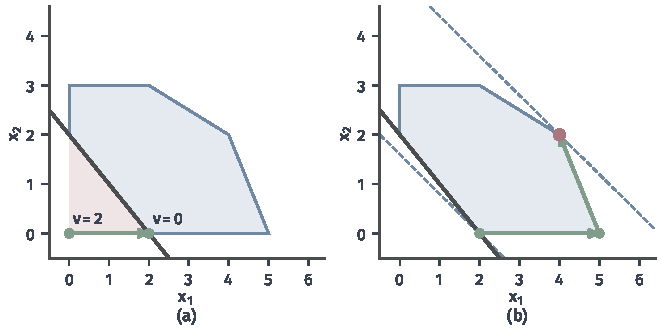
\includegraphics[width=112mm]{figures/05-optimization/01-linear-programming/matplotlib/simplex-two-phase-path/figure.pdf}
 \caption{两阶段法的路径。深灰粗线是合同约束$x_1+x_2=2$，浅蓝是原问题的可行域，它不含原点。(a)~第一阶段：从不可行的原点出发（红色浅底是违约区），沿$x_1$轴走到人工变量$v=x_7$降为零的点。(b)~第二阶段：从$(2,0)$出发，用原目标走到红色的最优点，蓝色虚线是利润$8$和$26$的等值线。}
 \label{fig:simplex-two-phase-path}
\end{BookInlineFigure}

\paragraph{第一阶段判定不可行}
把合同改成$x_1+x_2\geq7$。第一阶段从$\phi=7$开始，三轮的基和人工变量值为
\[
 \begin{aligned}
 B^{(0)}&=(3,4,5,7),& x_7&=7,\\
 B^{(1)}&=(3,1,5,7),& x_7&=2,\\
 B^{(2)}&=(2,1,5,7),& x_7&=1.
 \end{aligned}
\]
第$2$轮的对偶候选和约化成本是
\[
 \bm{y}=\Bigl(-\frac13,-\frac13,0,1\Bigr)^\top,\qquad
 s_3=\frac13,\quad s_4=\frac13,\quad s_6=1.
\]
全部非负而$\phi^\star=1>0$，原问题不可行。

证书$\bm{y}$可以翻译成一句平常的话。原料和工时两个约束各乘$\frac13$相加，得到$x_1+x_2\leq6$，这与$x_1+x_2\geq7$矛盾，差额正好是$\phi^\star=1$。图~\ref{fig:simplex-phase-one-infeasible}中，第一阶段把点推到离合同线最近的顶点，停在那里，仍差$1$。

\begin{BookInlineFigure}
 \centering
 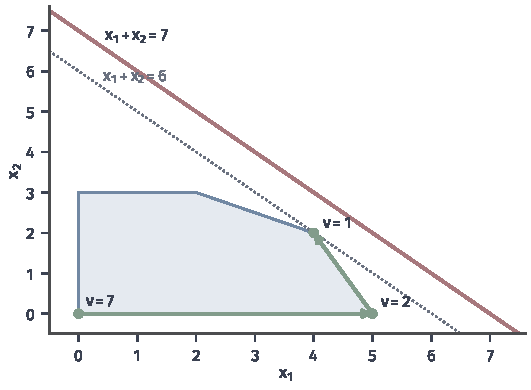
\includegraphics[width=90mm]{figures/05-optimization/01-linear-programming/matplotlib/simplex-phase-one-infeasible/figure.pdf}
 \caption{合同要求提高到$x_1+x_2\geq7$时的第一阶段。红线是合同边界，点线$x_1+x_2=6$是资源约束组合出的上限，两者之间没有可行点。绿色路径沿资源多边形的边界推进，人工变量$v$依次取$7,2,1$，在第一阶段最优点停在$v=1$。}
 \label{fig:simplex-phase-one-infeasible}
\end{BookInlineFigure}

\paragraph{基中残留的人工变量}
$\phi^\star=0$时，人工变量的值全为零，但可能有个别人工变量仍在基中，取值为零。第二阶段不能直接开始，否则人工变量可能在后续换基中重新变正。设它位于基的第$r$个位置，定义该行的系数
\begin{equation}
 \bm{\rho}=\bm{A}_B^{-\top}\bm{e}_r,\qquad \bar{a}_{r,j}=\bm{\rho}^\top\bm{a}_j,
 \label{eq:simplex-row-coefficients}
\end{equation}
其中$\bm{e}_r$是第$r$个坐标向量，$\bar{a}_{r,j}$就是把$\bm{a}_j$用基表示时第$r$个分量。分两种情况处理。

\begin{itemize}
 \item 存在原变量$x_j$（$j\in N$）使$\bar{a}_{r,j}\neq0$。把$x_j$换入第$r$个位置。由于该位置的值是零，步长为零，其他变量不变，符号不必为正。
 \item 对所有原变量都有$\bar{a}_{r,j}=0$。此时$\bm{\rho}^\top\bm{A}=\bm{0}^\top$，$\bm{\rho}\neq\bm{0}$，说明这一行是其余行的线性组合，是冗余等式，可以连同该人工变量一起删去。
\end{itemize}

第二种情况也说明，第~\ref{chap:linear-programming}章假定$\bm{A}$满行秩并不需要预先检查，第一阶段顺带就发现了冗余行。下面的例子展示两种情况。

\begin{example}[换出与删行]
 \label{ex:simplex-residual-artificial}
 考虑约束$x_1+x_2+x_3=2$，$2x_1+\omega(x_2+x_3)=4$，$\bm{x}\geq\bm{0}$，其中$\omega$取$1$或$2$，人工变量是$x_4,x_5$。从基$(4,5)$出发，$x_1$的约化成本最负。比值都是$2$，并列时取下标小的$x_4$出基，得到基$(1,5)$和
 \[
  \bm{x}_B=(2,0)^\top,\qquad \phi=0,\qquad\bm{\rho}=(-2,1)^\top.
 \]
 $x_5$在基中取零。

 取$\omega=1$时，系数是$\bar{a}_{2,2}=\bar{a}_{2,3}=-1\neq0$，把$x_2$换入第$2$个位置，步长为零，基变为$(1,2)$。

 取$\omega=2$时，系数是$\bar{a}_{2,2}=\bar{a}_{2,3}=0$。第二行正是第一行的$2$倍，删去第二行和$x_5$，基变为$(1)$。
\end{example}

图~\ref{fig:simplex-phase-flow}把两阶段法的分支整理在一起。

\begin{BookInlineFigure}
 \centering
 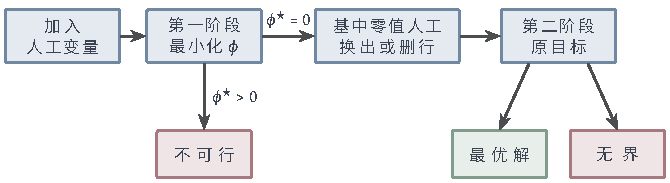
\includegraphics[width=112mm]{figures/05-optimization/01-linear-programming/tikz/simplex-phase-flow/figure.pdf}
 \caption{两阶段法的流程。第一阶段的最优值$\phi^\star$决定是否继续；基中取零的人工变量换出或连同冗余行删去后，第二阶段以原目标运行，以最优解或无界方向结束。红框是给出证书的否定结果，绿框是得到最优解。}
 \label{fig:simplex-phase-flow}
\end{BookInlineFigure}

\subsection{大M法}
\label{sec:simplex-big-m}

\paragraph{主要思想}
\term{大M法}（big-M method）把两个阶段合成一个问题，在目标中给人工变量定一个极高的单价：
\begin{equation}
 \min_{\bm{x},\bm{v}}\ \bm{c}^\top\bm{x}+M\,\bm{1}^\top\bm{v}
 \quad\text{s.t.}\quad
 \bm{A}\bm{x}+\bm{v}=\bm{b},\quad\bm{x}\geq\bm{0},\quad\bm{v}\geq\bm{0}.
 \label{eq:simplex-big-m}
\end{equation}
把$M$当作一个比任何数都大的符号来计算，约化成本就是形如$\beta+\gamma M$的式子，比较大小时先比$\gamma$，再比$\beta$。这样，只要还能减少人工变量，算法就不会先去改善原目标，排除人工变量自动享有优先权。

例中第$0$轮的对偶候选和约化成本是
\[
 \bm{y}=(0,0,0,M)^\top,\quad s_1=-4-M,\quad s_2=-5-M,\quad s_6=M.
\]
$s_1,s_2$里$M$的系数相同，再比常数项，$s_2$更负，$x_2$入基。此后各轮的数据在表~\ref{tab:simplex-big-m-rounds}中，路径见图~\ref{fig:simplex-big-m}(a)。第$0$轮换基后人工变量已经出基，接下来就是用原目标继续。

\begin{BookInlineTable}
 \centering
 \begin{tabular}{cccc}
  \toprule
  $t$ & $B^{(t)}$ & $(x_1,x_2)$ & 负的约化成本（入基）\\
  \midrule
  $0$ & $(3,4,5,7)$ & $(0,0)$ & $s_2=-5-M$，$s_1=-4-M$\\
  $1$ & $(3,4,5,2)$ & $(0,2)$ & $s_6=-5$\\
  $2$ & $(3,4,6,2)$ & $(0,3)$ & $s_1=-4$\\
  $3$ & $(1,4,6,2)$ & $(2,3)$ & $s_5=-3$\\
  $4$ & $(1,5,6,2)$ & $(4,2)$ & 无，停止\\
  \bottomrule
 \end{tabular}
 \caption{符号化大M法的各轮数据。}
 \label{tab:simplex-big-m-rounds}
\end{BookInlineTable}

\paragraph{有限的$M$要多大}
实际计算若取一个具体的数$M$，就必须问它够不够大。下面的定理给出精确的条件。

\begin{theorem}[有限惩罚的充分条件]
 \label{thm:simplex-finite-penalty}
 设标准型~\eqref{eq:simplex-standard-form}有最优解，最优值为$p^\star$，$\bm{y}^\star$是一个对偶最优解。若
 \begin{equation}
  M>\max_i\,y_i^\star,
  \label{eq:simplex-big-m-threshold}
 \end{equation}
 其中$i$取遍带人工变量的行，则问题~\eqref{eq:simplex-big-m}的最优值等于$p^\star$，并且它的每个最优解都满足$\bm{v}=\bm{0}$，其$\bm{x}$部分是原问题的最优解。
\end{theorem}

\begin{proof}
 为简洁起见设每行都有人工变量，其余情形只需令相应$v_i=0$。任取问题~\eqref{eq:simplex-big-m}的可行点$(\bm{x},\bm{v})$，记对偶松弛为$\bm{s}^\star\geq\bm{0}$，它满足$\bm{c}=\bm{s}^\star+\bm{A}^\top\bm{y}^\star$。把$\bm{c}$代换掉，并用$\bm{A}\bm{x}=\bm{b}-\bm{v}$，得到
 \[
  \bm{c}^\top\bm{x}
  =(\bm{s}^\star)^\top\bm{x}+(\bm{y}^\star)^\top\bm{A}\bm{x}
  \geq(\bm{y}^\star)^\top\bm{b}-(\bm{y}^\star)^\top\bm{v}.
 \]
 由强对偶，$\bm{b}^\top\bm{y}^\star=p^\star$，于是两边加上$M\bm{1}^\top\bm{v}$后，
 \[
  \bm{c}^\top\bm{x}+M\bm{1}^\top\bm{v}
  \geq p^\star+\sum_i(M-y_i^\star)v_i\geq p^\star.
 \]
 原问题的最优解配上$\bm{v}=\bm{0}$可行且取到$p^\star$，所以最优值是$p^\star$。若某个最优解有$v_i>0$，由式~\eqref{eq:simplex-big-m-threshold}上面最后一个不等号严格成立，与最优值为$p^\star$矛盾，所以$\bm{v}=\bm{0}$。此时$\bm{x}$可行且目标为$p^\star$，是原问题的最优解。
\end{proof}

门槛是对偶价格，这很合理：$y_i^\star$是放松第$i$条约束一单位时目标能下降多少，$M$是违反一单位约束要付的罚款。罚款高过这个收益，违约才不划算。

这个门槛取决于事先并不知道的$\bm{y}^\star$。把工厂的目标换成最小化成本$2x_1+3x_2$，合同约束就变成活动约束，最优解是$(2,0)$，对偶分量$y_4^\star=2$。图~\ref{fig:simplex-big-m}(b)对每个$M$精确求解，$M<2$时最优解干脆不生产，留着$v=2$付罚款，$M>2$时才回到真正的解。

\begin{BookInlineFigure}
 \centering
 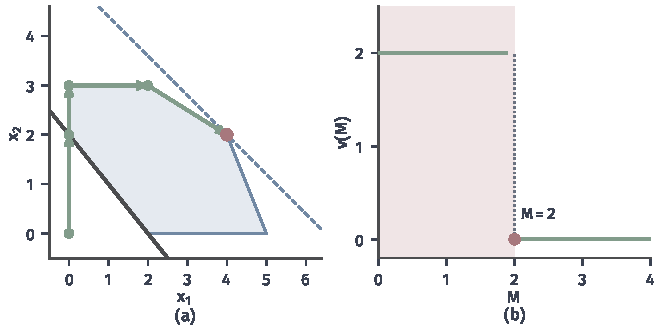
\includegraphics[width=112mm]{figures/05-optimization/01-linear-programming/matplotlib/simplex-big-m/figure.pdf}
 \caption{大M法。(a)~符号化大M在资源配置问题上的路径（绿色），第一步消去人工变量到达$(0,2)$，其后沿边界到最优点。(b)~目标$2x_1+3x_2+Mv$在不同有限$M$下的最优人工变量值$v(M)$：红色浅底的$M<2$区间内罚款不足，解停留在$v=2$；$M=2$时两种解并列（点线）；$M>2$时$v=0$。}
 \label{fig:simplex-big-m}
\end{BookInlineFigure}

$M$也不能随意取大。在双精度浮点数中，$10^{17}$附近相邻两个可表示数相差$16$，于是
\[
 -4-10^{17}\quad\text{和}\quad-5-10^{17}
\]
舍入后是同一个数，$c_1=-4$与$c_2=-5$的差别被抹掉，定价失去依据。系数相差过于悬殊还会使基矩阵病态。所以有限$M$不能靠“取一个很大的常数”得到保证；另外，若某个有限$M$的解有$v\neq\bm{0}$，也分不清是$M$不够大还是原问题不可行。

表~\ref{tab:simplex-two-phase-vs-big-m}对照了两种做法。

\begin{BookInlineTable}
 \centering
 \begin{tabular}{lll}
  \toprule
  & 两阶段法 & 大M法\\
  \midrule
  目标 & 先最小化$\bm{1}^\top\bm{v}$，再用$\bm{c}$ & 同时用$\bm{c}+M$惩罚\\
  不可行判定 & $\phi^\star>0$ & 符号化时$\bm{v}$不能消去\\
  参数 & 无 & 需要符号或足够大的$M$\\
  数值风险 & 无额外系数 & $M$过大使尺度恶化\\
  \bottomrule
 \end{tabular}
 \caption{两阶段法与大M法的对照。}
 \label{tab:simplex-two-phase-vs-big-m}
\end{BookInlineTable}

\section{退化的处理}
\label{sec:simplex-degeneracy}

定理~\ref{thm:simplex-finite-nondegenerate}的有限终止依赖一个假设：每次换基都能真正走出去。本节研究这个假设不成立时算法会发生什么，以及怎样修补。

\paragraph{同一个顶点，不同的基}
把工厂的工时从$10$改成$7$，三条约束边界就同时经过点$(2,3)$，如图~\ref{fig:simplex-degenerate-vertex}(a)所示。二维平面上确定一个点只需要两条线，这里却有三条，选哪两条都行。对应到代数上，这个点的$x_3=x_4=x_5=0$，三个变量中必须有一个留在基中，取值为零。这就是退化：一个基本可行解有基变量取零，同一个点可以对应多个基。

\begin{BookInlineFigure}
 \centering
 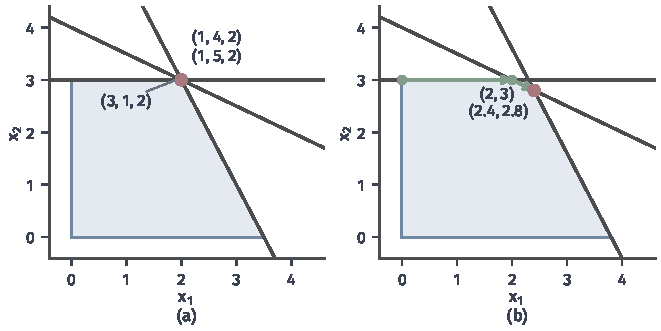
\includegraphics[width=112mm]{figures/05-optimization/01-linear-programming/matplotlib/simplex-degenerate-vertex/figure.pdf}
 \caption{退化顶点及其扰动。(a)~工时取$7$时三条约束边界（深灰）交于红点$(2,3)$，旁边的三元组是对应这同一个点的三个基。(b)~把工时夸张地增大到$7.6$后，这个顶点分裂成$(2,3)$和$(2.4,2.8)$两个相邻顶点，绿色路径多走一条真实的短边，每步都有实际移动。}
 \label{fig:simplex-degenerate-vertex}
\end{BookInlineFigure}

\paragraph{不移动的换基}
从基$(3,4,5)$开始运行Dantzig规则，前一轮与之前相同，$x_2$入基，点到$(0,3)$，基是$(3,4,2)$，$\bm{x}_B=(2,4,3)^\top$。下一轮$x_1$入基，$\bm{u}=(1,2,0)^\top$，两个比值并列：
\[
 \frac{2}{1}=2,\qquad \frac{4}{2}=2.
\]
这里的并列正是退化的来源：两个基变量同时降到零，只有一个能出基，另一个留下来取零。按下标小的规则，$x_3$出基，得到
\[
 B=(1,4,2),\qquad \bm{x}_B=(2,0,3)^\top,\qquad f=-23,
\]
点到达$(2,3)$。

此时的对偶候选和约化成本是
\[
 \bm{y}=(-4,0,3)^\top,\qquad s_3=4,\qquad s_5=-3.
\]
$s_5<0$，判别说还不能停。$x_5$入基，$\bm{u}=(-2,3,1)^\top$，比值是
\[
 \frac{x_4}{u_2}=\frac{0}{3}=0,\qquad \frac{x_2}{u_3}=\frac{3}{1}=3.
\]
步长$\alpha=0$，基变成$(1,5,2)$，点和目标都没变。新基的对偶候选和约化成本是
\[
 \bm{y}=(-2,-1,0)^\top,\qquad s_3=2,\qquad s_4=1,
\]
全部非负，算法才停下。

其实$(2,3)$早已是最优点，这一轮换基只是把基换成能出示证书的那一个。如果上一轮并列时让$x_4$出基，就直接得到基$(3,1,2)$，此时$\bm{y}=(0,-2,-3)^\top$，$s_4=2$，$s_5=3$，立即停止。这说明两点：退化基上$s_j<0$并不表示当前点不是最优；证书依赖基，同一个最优点上有的基能给出证书，有的基不能。

\paragraph{循环}
既然目标可以不下降，“每步都变好”的论证就失效了，算法可能在一组基之间兜圈子，这称为\term{循环}（cycling）。下面是一个有三行四个决策变量的例子，$x_5,x_6,x_7$是松弛变量：
\begin{equation}
 \begin{aligned}
 \min\quad & -10x_1+57x_2+9x_3+24x_4\\
 \text{s.t.}\quad & \tfrac12x_1-\tfrac{11}{2}x_2-\tfrac52x_3+9x_4+x_5=0,\\
 & \tfrac12x_1-\tfrac32x_2-\tfrac12x_3+x_4+x_6=0,\\
 & x_1+x_7=1,\qquad \bm{x}\geq\bm{0}.
 \end{aligned}
 \label{eq:simplex-cycling-example}
\end{equation}
用Dantzig规则，比值并列时取下标最小者，从基$(5,6,7)$出发，得到表~\ref{tab:simplex-cycling-rounds}的序列。每一步都有负的约化成本，每一步的步长都是零，第$6$步回到起点。

\begin{BookInlineTable}
 \centering
 \begin{tabular}{ccccc}
  \toprule
  $t$ & $B^{(t)}$ & 入基 & 约化成本 & 出基\\
  \midrule
  $0$ & $(5,6,7)$ & $x_1$ & $-10$ & $x_5$\\
  $1$ & $(1,6,7)$ & $x_2$ & $-53$ & $x_6$\\
  $2$ & $(1,2,7)$ & $x_3$ & $-29/2$ & $x_1$\\
  $3$ & $(3,2,7)$ & $x_4$ & $-18$ & $x_2$\\
  $4$ & $(3,4,7)$ & $x_5$ & $-21/2$ & $x_3$\\
  $5$ & $(5,4,7)$ & $x_6$ & $-24$ & $x_4$\\
  $6$ & $(5,6,7)$ & 回到第$0$轮 & & \\
  \bottomrule
 \end{tabular}
 \caption{问题~\eqref{eq:simplex-cycling-example}在Dantzig规则下的循环。}
 \label{tab:simplex-cycling-rounds}
\end{BookInlineTable}

图~\ref{fig:simplex-cycle-bases}把这六个基画成一个环。这个环上$\bm{x}$从未变化，所以只看目标值的话，看不出算法在做什么。

\begin{BookInlineFigure}
 \centering
 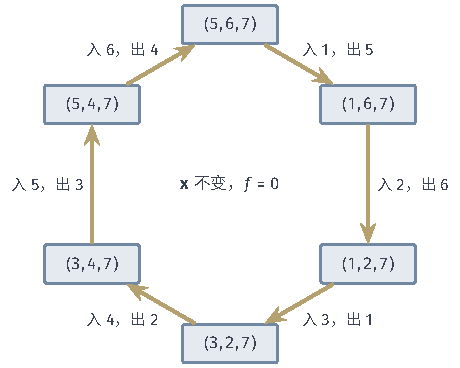
\includegraphics[width=78mm]{figures/05-optimization/01-linear-programming/tikz/simplex-cycle-bases/figure.pdf}
 \caption{问题~\eqref{eq:simplex-cycling-example}的六个基组成的循环。方框是基，黄色箭头是Dantzig规则下的一次换基，箭头旁写明入基和出基下标。整个环上$\bm{x}$和目标值都不变。}
 \label{fig:simplex-cycle-bases}
\end{BookInlineFigure}

\paragraph{Bland规则}
要打破循环，只需把“选哪一个”的自由度用一条固定的规则收走。\term{Bland规则}（Bland's rule）规定：入基变量取所有$s_j<0$中下标最小的；比值检验并列时，出基变量取下标最小的\scite{math-bland1977finite}。

\begin{theorem}[Bland规则的有限终止]
 \label{thm:simplex-bland}
 在精确算术下，使用Bland规则的单纯形法不会循环，因而经过有限次换基后停止。
\end{theorem}

\begin{proof}
 假设出现循环。目标值不增，循环中目标必须保持不变，所以每一步的步长都是零，$\bm{x}$在整个循环中不变，记为$\bar{\bm{x}}$。

 称循环中曾经入基的下标为活跃下标，活跃下标也必定曾经出基。活跃下标在某个基中非基，所以对应的$\bar{x}_j=0$。设$k$是最大的活跃下标。取循环中$k$将要出基的一个基$B$，此时入基的是活跃下标$q<k$。再取循环中$k$将要入基的一个基$B'$，其约化成本记为$\bm{s}'$，对偶候选记为$\bm{y}'$。

 由基$B$和入基$q$按式~\eqref{eq:simplex-direction}构造方向$\bm{d}$，它满足
 \[
  \bm{A}\bm{d}=\bm{0},\qquad \bm{c}^\top\bm{d}=s_q<0.
 \]
 用$\bm{s}'=\bm{c}-\bm{A}^\top\bm{y}'$，得到
 \[
  (\bm{s}')^\top\bm{d}=\bm{c}^\top\bm{d}-(\bm{y}')^\top\bm{A}\bm{d}=s_q<0.
 \]
 因此存在下标$j$使$s'_jd_j<0$。

 这个$j$满足$j\notin B'$，因为$B'$的基变量$s'_j=0$；同时$d_j\neq0$，故$j\in B$或$j=q$。两种情况下$j$都在循环中某一时刻属于基或正要入基，而在$B'$非基，所以$j$是活跃下标，$j\leq k$。

 下面排除$j=k$。$k$在$B$中将要出基，说明$u_k>0$，$d_k<0$；而$k$在$B'$中将要入基，说明$s'_k<0$。于是$s'_kd_k>0$，所以$j\neq k$，只能$j<k$。

 Bland规则在$B'$选了$k$入基，这说明比$k$小的下标都没有负的约化成本，所以$s'_j\geq0$，结合$s'_jd_j<0$得到$s'_j>0$，$d_j<0$。特别地$j\neq q$，所以$j\in B$，且$u_j=-d_j>0$。又$j$活跃，$\bar{x}_j=0$，于是$j$的比值是$0$，与$k$的比值并列。$j<k$却没有被选中出基，这与Bland规则矛盾。

 不循环意味着基不重复，基的个数有限，所以换基只能进行有限次。
\end{proof}

证明的结构值得留意：用最大的活跃下标构造一个对偶上的矛盾，正是“取下标最小”这个规则使矛盾成立。这个规则的作用是保证有限，不是追求速度，它常常比Dantzig规则走更多步。

回到问题~\eqref{eq:simplex-cycling-example}，Bland规则的前$5$步与表~\ref{tab:simplex-cycling-rounds}相同。第$5$轮基是$(5,4,7)$，约化成本$s_1=-22$，$s_6=-24$。Dantzig规则选$s_6$回到起点，Bland规则选下标小的$x_1$，走出了循环。再换一次基后，$x_3$入基时唯一的比值来自$x_7$，$\alpha=1$，得到
\[
 \bm{x}=(1,0,1,0,2,0,0)^\top,\qquad f=-1,
\]
约化成本全部非负。图~\ref{fig:simplex-cycling-objective}对比了两种规则的目标值。

\begin{BookInlineFigure}
 \centering
 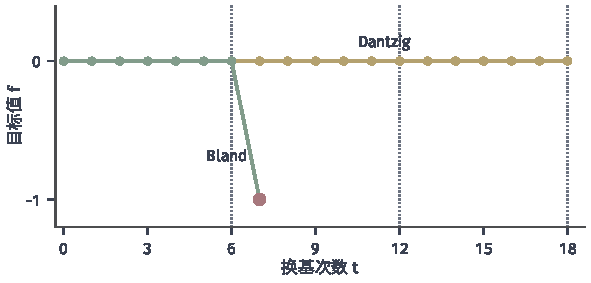
\includegraphics[width=100mm]{figures/05-optimization/01-linear-programming/matplotlib/simplex-cycling-objective/figure.pdf}
 \caption{问题~\eqref{eq:simplex-cycling-example}上两种规则的目标值。黄线是Dantzig规则，目标值恒为$0$，竖直点线标出每$6$步回到起始基；绿线是Bland规则，$6$次零步之后第$7$次换基走到红色的最优点，$f=-1$。}
 \label{fig:simplex-cycling-objective}
\end{BookInlineFigure}

\paragraph{字典序规则}
图~\ref{fig:simplex-degenerate-vertex}(b)提示了另一条路：既然麻烦来自几条约束恰好相交于一点，就把右端轻轻推开，让退化顶点裂成几个相距很近的普通顶点。把右端换成
\[
 \bm{b}+(\epsilon,\epsilon^2,\ldots,\epsilon^m)^\top,
\]
其中$\epsilon>0$充分小，比值并列就不会发生，每步都有严格的下降。

\term{字典序规则}（lexicographic rule）把这个想法做成不需要真的取$\epsilon$的规则：比值并列时，比较各并列行的向量$[\bar{x}_{B(i)},(\bm{A}_B^{-1})_{i,:}]/u_i$，取字典序最小者出基。它的作用等同于对无穷小的扰动做比值检验。证明需要跟踪各行字典序为正这一性质，并说明每次换基使目标行严格字典序下降，读者可查阅线性规划专著\scite{math-bertsimas1997linear}。结论同样是：在精确算术下不循环，有限终止。

两种规则的保证都建立在精确算术之上。浮点计算里，“恰好是零”没有意义，比值并列要用容差判断，舍入误差也会把退化基上的零扰动成微小的正负数。所以实现时除了防循环的规则，还要在最后重新核查可行性和约化成本，第~\ref{sec:simplex-revised}节将说明怎样做。

\section{修正单纯形法}
\label{sec:simplex-revised}

前面把算法写成了矩阵公式，每轮都出现$\bm{A}_B^{-1}$。接下来要弄清：真正计算时应该保存什么，每轮要做多少运算？

\paragraph{完整的单纯形表}
最直接的办法是把所有非基变量的表示都算出来，存成一张表。\term{单纯形表}（simplex tableau）的主体是$\bm{A}_B^{-1}[\bm{b}\ \ \bm{A}]$，再加一行约化成本。例中第$2$轮的基是$(1,4,2)$，表~\ref{tab:simplex-tableau}的上半部分就是这张表，每一列都是对应$\bm{a}_j$在当前基下的表示，$u$和$\bar{x}_B$都可以直接读出。

换基就是对这张表做一次Gauss--Jordan消元，主元取在出基行和入基列的交点。例中主元是$x_4$行$x_5$列的$3$。把该行除以$3$，再用它消去$x_5$列的其他元素，就得到下半部分，也就是第$3$轮的表。

\begin{BookInlineTable}
 \centering
 \begin{tabular}{crrrrrr}
  \toprule
  基 & $\bar{x}$ & $x_1$ & $x_2$ & $x_3$ & $x_4$ & $x_5$\\
  \midrule
  $x_1$ & $2$ & $1$ & $0$ & $1$ & $0$ & $-2$\\
  $x_4$ & $3$ & $0$ & $0$ & $-2$ & $1$ & $3$\\
  $x_2$ & $3$ & $0$ & $1$ & $0$ & $0$ & $1$\\
  $\bm{s}$ & $23$ & $0$ & $0$ & $4$ & $0$ & $-3$\\
  \midrule
  $x_1$ & $4$ & $1$ & $0$ & $-1/3$ & $2/3$ & $0$\\
  $x_5$ & $1$ & $0$ & $0$ & $-2/3$ & $1/3$ & $1$\\
  $x_2$ & $2$ & $0$ & $1$ & $2/3$ & $-1/3$ & $0$\\
  $\bm{s}$ & $26$ & $0$ & $0$ & $2$ & $1$ & $0$\\
  \bottomrule
 \end{tabular}
 \caption{资源配置问题第$2$轮（上）和第$3$轮（下）的单纯形表。第二列是基变量取值，$\bm{s}$行第二列是利润$-f$，其余是约化成本。}
 \label{tab:simplex-tableau}
\end{BookInlineTable}

这张表手算方便，但代价不小：每轮要更新大约$(m+1)(n+1)$个数，无论这一轮用到多少。而且$\bm{A}$稀疏时，$\bm{A}_B^{-1}\bm{A}$通常是稠密的，存储量也不可接受。

\paragraph{每轮真正需要什么}
回头看第~\ref{sec:simplex-basis-exchange}节的计算步骤，一轮只用到四样东西：解一次$\bm{A}_B^\top\bm{y}=\bm{c}_B$，用$\bm{y}$和$\bm{A}$的非基列做内积定价，对入基列解一次$\bm{A}_B\bm{u}=\bm{a}_q$，再做比值检验。表中其他列的表示从未被使用。\term{修正单纯形法}（revised simplex method）因此只维护基矩阵的因子，其余的量需要时再算。一轮的数据流如图~\ref{fig:simplex-revised-flow}所示。

\begin{BookInlineFigure}
 \centering
 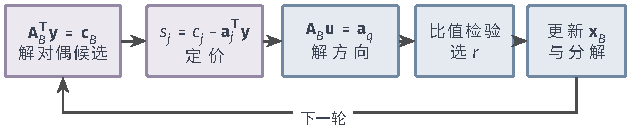
\includegraphics[width=107mm]{figures/05-optimization/01-linear-programming/tikz/simplex-revised-flow/figure.pdf}
 \caption{修正单纯形法一轮的数据流。紫色框处理对偶量：解$\bm{A}_B^\top\bm{y}=\bm{c}_B$得到对偶候选，再对非基列定价。蓝色框处理原始量：解$\bm{A}_B\bm{u}=\bm{a}_q$，比值检验选出基位置，更新基变量和基矩阵的因子。}
 \label{fig:simplex-revised-flow}
\end{BookInlineFigure}

\paragraph{基矩阵逆的更新}
相邻两轮的基矩阵只差一列，无需重新分解。设新基$B'$把第$r$列换成$\bm{a}_q$。由$\bm{a}_q=\bm{A}_B\bm{u}$，新基矩阵可以写成
\[
 \bm{A}_{B'}=\bm{A}_B\bm{F},
\]
其中$\bm{F}$是把单位矩阵第$r$列换成$\bm{u}$的矩阵。两边求逆，只需要$\bm{F}$的逆，它仍是单位矩阵只改第$r$列的形状：
\begin{equation}
 \bm{A}_{B'}^{-1}=\bm{E}\bm{A}_B^{-1},\qquad
 \bm{E}_{:,r}=\bm{\eta},\qquad
 \eta_i=
 \begin{cases}
  -u_i/u_r,& i\neq r,\\
  1/u_r,& i=r.
 \end{cases}
 \label{eq:simplex-eta-update}
\end{equation}
这样的$\bm{E}$只需保存一列，称为eta矩阵。

例中从第$2$轮到第$3$轮，$\bm{u}=(-2,3,1)^\top$，$r=2$，于是
\[
 \bm{E}=\begin{bmatrix}1&2/3&0\\0&1/3&0\\0&-1/3&1\end{bmatrix}.
\]
第$2$轮的基矩阵逆左乘$\bm{E}$，就得到第$3$轮的基矩阵逆：
\begin{equation}
 \bm{A}_{B^{(3)}}^{-1}
 =\bm{E}\begin{bmatrix}1&0&-2\\-2&1&3\\0&0&1\end{bmatrix}
 =\begin{bmatrix}-1/3&2/3&0\\-2/3&1/3&1\\2/3&-1/3&0\end{bmatrix}.
 \label{eq:simplex-final-inverse}
\end{equation}
这个矩阵的第$r$行就是式~\eqref{eq:simplex-row-coefficients}中的$\bm{\rho}$，后两节会反复用到它。

\paragraph{运算量的比较}
表~\ref{tab:simplex-implementation-costs}列出每轮的存储和运算。这里$\operatorname{nnz}(\cdot)$表示非零元个数。修正法的优势在$n\gg m$或$\bm{A}$稀疏时最明显：定价只碰$\bm{A}$的非零元，解方程只碰因子的非零元。

\begin{BookInlineTable}
 \centering
 \begin{tabular}{lll}
  \toprule
  实现方式 & 存储 & 每轮主要运算\\
  \midrule
  完整单纯形表 & $(m+1)(n+1)$ & 约$mn$次更新\\
  修正法，稠密逆 & $m^2$ & 约$m^2+\operatorname{nnz}(\bm{A})$\\
  修正法，LU加eta & 因子的非零元 & 两次三角回代加定价\\
  \bottomrule
 \end{tabular}
 \caption{单纯形法几种实现的每轮代价，均指量级。}
 \label{tab:simplex-implementation-costs}
\end{BookInlineTable}

\paragraph{稀疏性}
大规模问题的基矩阵往往非常稀疏，这时不应显式保存逆。图~\ref{fig:simplex-sparsity}是一个$40$阶三对角矩阵的例子。矩阵本身和它的LU因子都只有$118$个非零位置，而逆矩阵的$1600$个元素全部非零。实际软件保存基矩阵经过行列重排的LU分解，再累积一串eta矩阵，这也是用稀疏因子代替稠密逆的具体办法。重排的目的是减少分解过程中新产生的非零元；LU分解和三角回代的基本算法，可参考\BookChapterRef{chap:direct-linear-solvers}{卷二第12章“线性方程的直接求解”}。

\begin{BookInlineFigure}
 \centering
 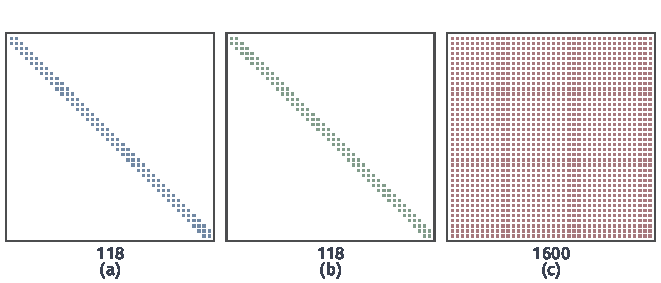
\includegraphics[width=112mm]{figures/05-optimization/01-linear-programming/matplotlib/simplex-sparsity/figure.pdf}
 \caption{$40$阶三对角基矩阵的非零结构，每个小点是一个非零元，图下的数字是非零元总数。(a)~矩阵本身。(b)~不选主元的LU因子合在一起，没有新增非零元。(c)~逆矩阵，全部$1600$个元素非零。}
 \label{fig:simplex-sparsity}
\end{BookInlineFigure}

\paragraph{舍入误差}
连续用eta矩阵更新，每一步都要除以$u_r$。若主元$u_r$很小，比如$10^{-12}$，$\bm{\eta}$的元素可达$10^{12}$量级，舍入误差被同比放大，并一直留在后续的所有计算里。图~\ref{fig:simplex-refactorization}是一个固定随机种子的实验：在$120$阶稠密随机基矩阵上连续换入随机列，比较选取不同主元的残差。总选最大的主元时残差始终在$10^{-13}$左右；总选合格主元中最小的那个时，残差上升好几个数量级，定期重新分解能把它拉回来，但只要继续用小主元，残差又会很快上升。

\begin{BookInlineFigure}
 \centering
 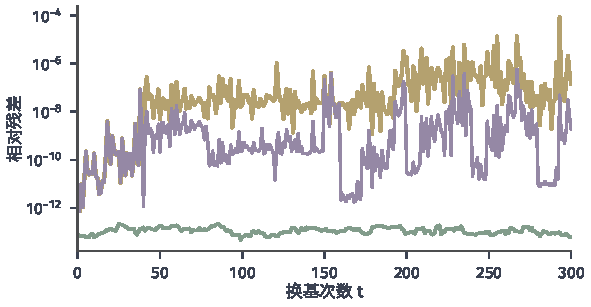
\includegraphics[width=100mm]{figures/05-optimization/01-linear-programming/matplotlib/simplex-refactorization/figure.pdf}
 \caption{用更新后的逆求$\bm{x}_B$时的相对残差$\lVert\bm{A}_B\bm{x}_B-\bm{b}\rVert_2/\lVert\bm{b}\rVert_2$，随机种子固定，矩阵阶数$120$。绿线每步选最大主元且不重分解；黄线每步选$\lvert u_r\rvert>10^{-4}$中最小的主元且不重分解；紫线的选法同黄线，但每$40$次换基重新计算一次逆。}
 \label{fig:simplex-refactorization}
\end{BookInlineFigure}

实验提示了实现时的几条具体做法。比值检验并列或接近并列时，优先选$\lvert u_r\rvert$大的主元，低于主元容差的不选。累积若干个eta矩阵后，重新分解$\bm{A}_B$，用新因子重算$\bm{x}_B,\bm{y},\bm{s}$。

浮点数下的“非负”也只能在容差内判断。常见的可行性容差在$10^{-9}$到$10^{-6}$之间，即接受$x_j\geq-\varepsilon$，约化成本用同样的方式判断。因此算法报告“最优”的含义是：在给定容差下，$\bm{A}\bm{x}=\bm{b}$的残差、$\bm{x}$的负部和$\bm{s}$的负部都足够小。收尾时应该用新的分解重算一遍这三个量，并做必要的尺度还原，因为这些容差是在内部缩放后的问题上判断的，换回原单位后需要另行核查。

\section{对偶单纯形法}
\label{sec:simplex-dual}

工厂解完问题后，资源情况变了：原料增加到$13$，工时骤减到$2$，设备增加到$4$。这就需要回答：手里的最优基还能怎样利用，而不必从头求解？

\paragraph{基的两种可行性}
约化成本只依赖$\bm{c}$和基，与$\bm{b}$无关。所以右端变化后，原来的最优基$(1,5,2)$依然满足$\bm{s}\geq\bm{0}$，也就是对偶可行。受影响的是基变量。用式~\eqref{eq:simplex-final-inverse}的逆矩阵计算，新的基变量是
\[
 \bm{x}_B=\bm{A}_B^{-1}\begin{bmatrix}13\\2\\4\end{bmatrix}=\begin{bmatrix}-3\\-4\\8\end{bmatrix}.
\]
基失去了原始可行性，而对偶可行性完好。这正好与上一节相反：原始单纯形法保持$\bm{x}_B\geq\bm{0}$，逐步争取$\bm{s}\geq\bm{0}$；现在我们手里是$\bm{s}\geq\bm{0}$，需要逐步争取$\bm{x}_B\geq\bm{0}$。\term{对偶单纯形法}（dual simplex method）做的就是这件事。

\paragraph{主要思想}
选一个$\bar{x}_{B(r)}<0$的位置，让这个基变量出基。写出第$r$行，由式~\eqref{eq:simplex-basic-form}和式~\eqref{eq:simplex-row-coefficients}，每个满足等式的点都有
\begin{equation}
 x_{B(r)}+\sum_{j\in N}\bar{a}_{r,j}x_j=\bar{x}_{B(r)}<0.
 \label{eq:simplex-dual-row}
\end{equation}
要把$x_{B(r)}$抬到零，必须让某个$\bar{a}_{r,j}<0$的非基变量变大。候选可能有好几个，选哪一个由对偶可行性决定。

换到对偶的角度看。沿方向$\bm{\rho}$改变对偶变量，令$\bm{y}(\tau)=\bm{y}-\tau\bm{\rho}$，$\tau\geq0$。第一，对偶目标增大，这是我们想要的：
\[
 \bm{b}^\top\bm{y}(\tau)=\bm{b}^\top\bm{y}-\tau\,\bar{x}_{B(r)},
\]
这里用到了$\bm{\rho}^\top\bm{b}=\bar{x}_{B(r)}$。第二，约化成本线性变化：
\begin{equation}
 s_j(\tau)=c_j-\bm{a}_j^\top\bm{y}+\tau\,\bm{a}_j^\top\bm{\rho}=s_j+\tau\,\bar{a}_{r,j}.
 \label{eq:simplex-dual-reduced-cost}
\end{equation}
其他基变量的$\bar{a}_{r,j}=0$，它们的约化成本保持为零；第$r$个基变量的$\bar{a}_{r,j}=1$，约化成本变为$\tau\geq0$。非基变量中$\bar{a}_{r,j}\geq0$的不会变差，$\bar{a}_{r,j}<0$的会下降，下降到零时就必须停止。这就是对偶的比值检验：
\begin{equation}
 \tau^\star=\min_{j\in N:\,\bar{a}_{r,j}<0}\frac{s_j}{-\bar{a}_{r,j}}.
 \label{eq:simplex-dual-ratio}
\end{equation}
取到最小值的$q$入基，它的约化成本恰好变成零，所有约化成本仍然非负。

对比原始比值检验：原始检验防止基变量变负，选最先碰零的基变量出基；对偶检验防止约化成本变负，选最先碰零的非基变量入基。两者结构完全对称。表~\ref{tab:simplex-primal-dual-comparison}列出这种对称。

\begin{BookInlineTable}
 \centering
 \begin{tabular}{lll}
  \toprule
  & 原始单纯形法 & 对偶单纯形法\\
  \midrule
  保持 & $\bm{x}_B\geq\bm{0}$ & $\bm{s}\geq\bm{0}$\\
  争取 & $\bm{s}\geq\bm{0}$ & $\bm{x}_B\geq\bm{0}$\\
  先选 & $s_q<0$，入基 & $\bar{x}_{B(r)}<0$，出基\\
  比值检验选 & 出基位置 & 入基下标\\
  目标值 & 单调下降 & 单调上升\\
  否定结论 & 无界 & 不可行\\
  \bottomrule
 \end{tabular}
 \caption{原始单纯形法与对偶单纯形法的对照。}
 \label{tab:simplex-primal-dual-comparison}
\end{BookInlineTable}

式~\eqref{eq:simplex-dual-row}也解释了没有候选时的结论。若所有$\bar{a}_{r,j}\geq0$，式~\eqref{eq:simplex-dual-row}左端对任何$\bm{x}\geq\bm{0}$都非负，右端却是负数，所以无解。

\begin{theorem}[对偶单纯形法的不可行证书]
 \label{thm:simplex-dual-infeasible}
 设$\bar{x}_{B(r)}<0$，且所有$j\in N$都有$\bar{a}_{r,j}\geq0$，则$\bm{A}\bm{x}=\bm{b}$，$\bm{x}\geq\bm{0}$无解，$\bm{\rho}$满足
 \begin{equation}
  \bm{A}^\top\bm{\rho}\geq\bm{0},\qquad \bm{b}^\top\bm{\rho}=\bar{x}_{B(r)}<0.
  \label{eq:simplex-dual-certificate}
 \end{equation}
\end{theorem}

\begin{proof}
 基列的$\bm{\rho}^\top\bm{a}_j$是$0$或$1$，非基列的$\bm{\rho}^\top\bm{a}_j=\bar{a}_{r,j}\geq0$，所以$\bm{A}^\top\bm{\rho}\geq\bm{0}$；$\bm{b}^\top\bm{\rho}$是$\bm{A}_B^{-1}\bm{b}$的第$r$个分量。若有可行点$\bm{x}$，则
 \[
  0\leq\bm{x}^\top\bm{A}^\top\bm{\rho}=\bm{b}^\top\bm{\rho}<0,
 \]
 矛盾。
\end{proof}

\needspace{6\baselineskip}
\paragraph{变量}
沿用原始单纯形法的$B^{(t)},\bm{x}_B^{(t)},\bm{y}^{(t)},\bm{s}^{(t)},\bm{u}^{(t)}$，另增下面的量。
\begin{itemize}
 \item $r^{(t)}$：出基位置，$p^{(t)}=B^{(t)}(r^{(t)})$是出基下标。
 \item $\bm{\rho}^{(t)}\in\mathbb{R}^m$：$\bm{A}_B^{-\top}\bm{e}_r$；$\bar{a}_{r,j}^{(t)}$：第$r$行对第$j$列的系数。
 \item $\tau^{(t)}\geq0$：对偶步长；$q^{(t)}$：入基下标；$\alpha^{(t)}$：原始步长。
\end{itemize}

\paragraph{初始化}
需要一个对偶可行基。例中取原来的最优基，数据由式~\eqref{eq:simplex-resource-dual}和上面的计算得到：
\[
 B^{(0)}=(1,5,2),\qquad \bm{x}_B^{(0)}=(-3,-4,8)^\top,\qquad \bm{y}^{(0)}=(-2,-1,0)^\top.
\]
约化成本是$s_3=2$，$s_4=1$，对偶目标$\bm{b}^\top\bm{y}^{(0)}=-28$。这个$-28$比原问题的最优值低，它是新问题最优值的一个下界，算法要把它抬高。

\needspace{6\baselineskip}
\paragraph{每轮更新}
第$t$轮依次做下面几步。步骤后的“例中”是第$0$轮的数据。
\begin{enumerate}

 \item 判别。若$\bm{x}_B^{(t)}\geq\bm{0}$，停止，当前解最优。否则选负分量位置$r$出基，常取最负的。例中最负的是$x_5=-4$：
 \[
  r^{(0)}=2,\qquad p^{(0)}=5.
 \]

 \item 计算第$r$行。由式~\eqref{eq:simplex-row-coefficients}，例中取式~\eqref{eq:simplex-final-inverse}的第$2$行：
 \[
  \bm{\rho}^{(0)}=\Bigl(-\frac23,\frac13,1\Bigr)^\top,\qquad
  \bar{a}_{2,3}=-\frac23,\qquad \bar{a}_{2,4}=\frac13.
 \]

 \item 对偶比值检验。若所有$\bar{a}_{r,j}\geq0$，停止，按定理~\ref{thm:simplex-dual-infeasible}报告不可行。否则由式~\eqref{eq:simplex-dual-ratio}确定$\tau^{(t)}$和$q^{(t)}$。例中只有$x_3$是候选：
 \[
  \tau^{(0)}=\frac{2}{2/3}=3,\qquad q^{(0)}=3.
 \]

 \item 更新对偶量。沿$\bm{\rho}$移动，由式~\eqref{eq:simplex-dual-reduced-cost}更新约化成本：
 \begin{equation}
  \bm{y}^{(t+1)}=\bm{y}^{(t)}-\tau^{(t)}\bm{\rho}^{(t)},\qquad
  s_j^{(t+1)}=s_j^{(t)}+\tau^{(t)}\bar{a}_{r,j}^{(t)}.
  \label{eq:simplex-dual-update}
 \end{equation}
 例中
 \[
  \bm{y}^{(1)}=(0,-2,-3)^\top,\qquad s_4^{(1)}=1+3\cdot\frac13=2,\qquad s_5^{(1)}=3.
 \]

 \item 更新原始量。先求$\bm{u}^{(t)}=\bm{A}_B^{-1}\bm{a}_q$，取原始步长$\alpha^{(t)}=\bar{x}_{B(r)}/\bar{a}_{r,q}$，它是让第$r$个基变量恰好变成零的步长。其余基变量按式~\eqref{eq:simplex-primal-update}更新，第$r$个位置放$x_q=\alpha^{(t)}$。例中
 \[
  \bm{u}^{(0)}=\Bigl(-\frac13,-\frac23,\frac23\Bigr)^\top,\qquad
  \alpha^{(0)}=\frac{-4}{-2/3}=6.
 \]
 于是
 \[
  B^{(1)}=(1,3,2),\qquad \bm{x}_B^{(1)}=(-1,6,4)^\top,\qquad \bm{b}^\top\bm{y}^{(1)}=-16.
 \]
\end{enumerate}

例中第$1$轮只剩$x_1=-1$为负，所以$r=1$，$x_1$出基。第$1$行的系数和唯一的候选是
\[
 \bm{\rho}^{(1)}=\Bigl(0,\frac12,-\frac12\Bigr)^\top,\qquad
 \bar{a}_{1,4}=\frac12,\qquad \bar{a}_{1,5}=-\frac12,\qquad
 \tau^{(1)}=\frac{3}{1/2}=6.
\]
于是$x_5$入基，由式~\eqref{eq:simplex-dual-update}得到
\[
 \bm{y}^{(2)}=(0,-5,0)^\top,\qquad s_1^{(2)}=6,\qquad s_4^{(2)}=2+6\cdot\frac12=5.
\]
原始量的更新用
\[
 \bm{u}^{(1)}=\Bigl(-\frac12,-\frac32,1\Bigr)^\top,\qquad
 \alpha^{(1)}=\frac{-1}{-1/2}=2,
\]
更新后得到
\[
 B^{(2)}=(5,3,2),\qquad \bm{x}_B^{(2)}=(2,9,2)^\top,\qquad \bm{b}^\top\bm{y}^{(2)}=-10.
\]
第$2$轮$\bm{x}_B\geq\bm{0}$，算法停止。

\paragraph{最终得到}
新问题的最优解和最优值是
\[
 (x_1,x_2)=(0,2),\qquad p^\star=-10.
\]
工时只有$2$，全部给利润率更高的产品二最合算。对偶目标依次是$-28,-16,-10$，每一步增加$\tau\lvert\bar{x}_{B(r)}\rvert$，即$3\cdot4=12$和$6\cdot1=6$，它们一直是最优值的下界，到达时恰好等于最优值。这与第~\ref{sec:simplex-basis-exchange}节目标从上方下降的情形相反。

图~\ref{fig:simplex-dual-path}(a)显示了路径的特点：前两个点$(-3,8)$和$(-1,4)$都在可行域之外，它们是一系列“太便宜而不可能达到”的解，算法一步步向可行域靠拢，碰到可行域时恰好最优。

\begin{BookInlineFigure}
 \centering
 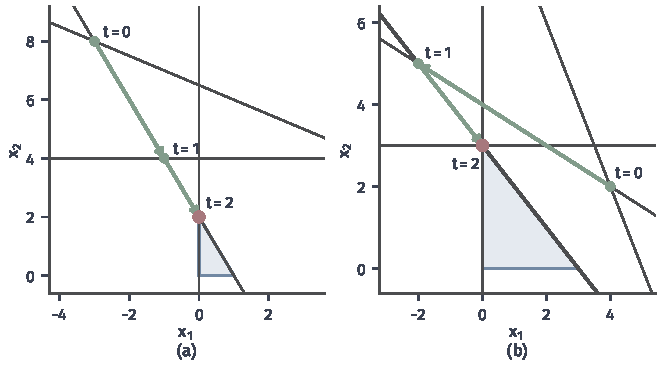
\includegraphics[width=112mm]{figures/05-optimization/01-linear-programming/matplotlib/simplex-dual-path/figure.pdf}
 \caption{对偶单纯形法在原始空间的路径（绿色），深灰线是约束边界，浅蓝是可行域，红点是最优解。(a)~右端变为$(13,2,4)$后，从不可行点$(-3,8)$经$(-1,4)$到$(0,2)$。(b)~新增约束$x_1+x_2\leq3$（粗线）后，从原最优点$(4,2)$经不可行点$(-2,5)$到$(0,3)$。}
 \label{fig:simplex-dual-path}
\end{BookInlineFigure}

\paragraph{新增约束与基的复用}
加入新约束是另一种常见的情形。给工厂加一条约束$x_1+x_2\leq3$，并引入松弛变量$x_6$。把$x_6$放入基，原最优基扩展成$(1,5,2,6)$。新基对偶可行，因为新列只增加一个取零的约化成本；只有$x_6$可能违反非负，这里$x_6=3-6=-3$。

第$0$轮$x_6$出基，第$4$行的系数和两个候选比值是
\[
 \bar{a}_{4,3}=-\frac13,\qquad \bar{a}_{4,4}=-\frac13,\qquad
 \frac{2}{1/3}=6,\qquad \frac{1}{1/3}=3.
\]
图~\ref{fig:simplex-dual-ratio}把这两个比值画成约化成本随$\tau$下降的直线，$s_4$先碰到零，所以$x_4$入基。再经一轮换基，$\bm{x}_B$全部非负，得到$(x_1,x_2)=(0,3)$，利润$15$。

\begin{BookInlineFigure}
 \centering
 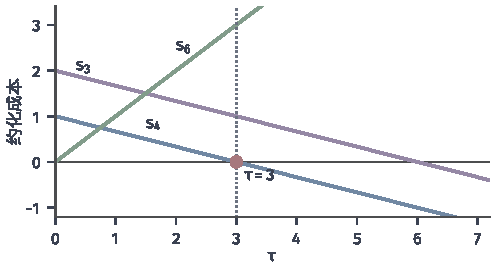
\includegraphics[width=84mm]{figures/05-optimization/01-linear-programming/matplotlib/simplex-dual-ratio/figure.pdf}
 \caption{新增约束后第$0$轮的对偶比值检验。三条直线是约化成本随对偶步长$\tau$的变化：$s_3=2-\tau/3$，$s_4=1-\tau/3$，$s_6=\tau$。红点是最先降到零的位置$\tau=3$，它决定入基变量$x_4$；$s_6$对应出基的$x_6$，只增不减。}
 \label{fig:simplex-dual-ratio}
\end{BookInlineFigure}

如果新增的约束与资源不相容，比如$x_1+x_2\geq7$，化为$-x_1-x_2+x_6=-7$后，第一轮$x_6=-1$，第$4$行是
\[
 x_6+\frac13x_3+\frac13x_4=-1.
\]
系数全部非负而右端为负，这正是定理~\ref{thm:simplex-dual-infeasible}的情形，算法一步报告不可行。这和第~\ref{sec:simplex-two-phase}节第一阶段得到的结论相同，证书都是原料和工时约束的组合。

这种利用已有基的做法称为\term{热启动}（warm start）。它是整数规划算法的基本工序：分支限界在线性松弛的解上增加一个变量界，割平面增加一条被当前解违反的不等式，两者都只在原问题上添一点约束，原来的最优基仍然对偶可行。对偶单纯形法往往只需少量换基就能恢复可行，比从头求解省得多。热启动的效果依赖新约束对解的改变有多大，并没有通用的步数保证。

\section{固定基的参数分析}
\label{sec:simplex-parametric}

上一节处理了参数变化之后怎样重新求解。本节问得更早一步：参数在多大范围内变化时，原来的最优基根本不用换，最优解和最优值又怎样随参数变化。

固定最优基$B^\star=(1,5,2)$。式~\eqref{eq:simplex-final-inverse}给出了它的逆矩阵，所有结论都来自这个矩阵。基保持最优需要两个条件：$\bm{x}_B\geq\bm{0}$保证原始可行，$\bm{s}\geq\bm{0}$保证对偶可行。右端变化只影响前者，目标系数变化只影响后者。

\paragraph{右端变化}
设第$i$个资源变化$\delta$，即$\bm{b}(\delta)=\bm{b}+\delta\bm{e}_i$。基不变时，基变量和目标值都是$\delta$的线性函数：
\begin{equation}
 \bm{x}_B(\delta)=\bar{\bm{x}}_B+\delta\,\bm{A}_B^{-1}\bm{e}_i,
 \qquad
 f(\delta)=p^\star+\delta\,y_i.
 \label{eq:simplex-rhs-parametric}
\end{equation}
第二个式子由$f=\bm{b}^\top\bm{y}$和$\bm{y}$不随$\bm{b}$变化得到。基保持可行的条件是$\bm{x}_B(\delta)\geq\bm{0}$，这是对$\delta$的一组线性不等式，解出来是一个区间。

以原料$b_1=8+\delta$为例，$\bm{A}_B^{-1}\bm{e}_1$是式~\eqref{eq:simplex-final-inverse}的第一列，于是
\[
 x_1=4-\frac13\delta,\qquad
 x_5=1-\frac23\delta,\qquad
 x_2=2+\frac23\delta.
\]
三个非负条件分别要求
\[
 \delta\leq12,\qquad \delta\leq\frac32,\qquad \delta\geq-3.
\]
取交集，$\delta\in[-3,3/2]$，也就是$b_1\in[5,9.5]$。图~\ref{fig:simplex-rhs-range}(a)展示了这个范围的几何意义：$b_1$变化时，原料线平行移动，最优顶点沿工时线滑动，下端碰到$x_2=0$，上端碰到设备约束，再走基就要换了。

\begin{BookInlineFigure}
 \centering
 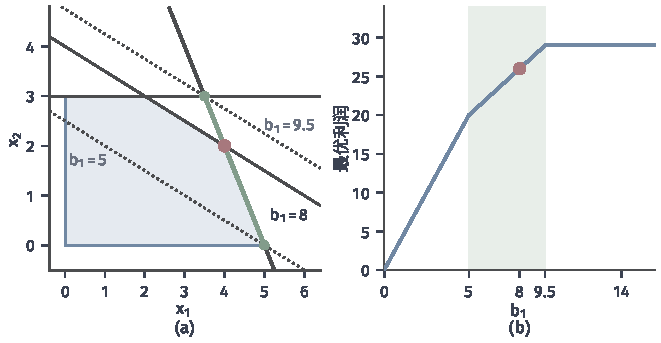
\includegraphics[width=112mm]{figures/05-optimization/01-linear-programming/matplotlib/simplex-rhs-range/figure.pdf}
 \caption{原料$b_1$的有效范围。(a)~实线和点线是$b_1=8$及范围两端$b_1=5,9.5$的原料线，绿色线段是最优顶点随$b_1$滑过的路径，红点是$b_1=8$的最优点。(b)~最优利润随$b_1$的变化（蓝线，对每个$b_1$精确求解），绿色底是基$(1,5,2)$的有效范围，其中斜率恒为影子价格$2$，范围之外斜率改变。}
 \label{fig:simplex-rhs-range}
\end{BookInlineFigure}

\paragraph{影子价格}
在有效范围内，$y_i$就是目标对$b_i$的变化率。按最大化利润的语言，它的相反数是多一单位资源带来的额外利润，称为\term{影子价格}（shadow price）。例中
\[
 -y_1^\star=2,\qquad -y_2^\star=1,\qquad -y_3^\star=0.
\]
一单位原料值$2$，一单位工时值$1$，设备还有富余，增加设备不值钱。如果市场上原料的单价低于$2$，就值得购买，但这个判断只在$b_1\leq9.5$之内有效。超过这个范围，图~\ref{fig:simplex-rhs-range}(b)的斜率变成了$0$，因为此时专用设备成了新的瓶颈。“影子价格”是局部的，它是某个固定基上的数，不是资源的绝对价值。

\paragraph{目标系数变化}
设基变量$x_k$的成本变化$\delta$，$k=B(\ell)$，$\bm{c}(\delta)=\bm{c}+\delta\bm{e}_k$。此时$\bm{x}$不变，对偶候选变化，由式~\eqref{eq:simplex-reduced-cost}计算得到
\begin{equation}
 s_j(\delta)=s_j-\delta\,\bar{a}_{\ell,j}\quad(j\in N),
 \qquad
 f(\delta)=p^\star+\delta\,x_k^\star.
 \label{eq:simplex-cost-parametric}
\end{equation}
其中$\bar{a}_{\ell,j}$是第$\ell$行的系数。基保持最优的条件是$s_j(\delta)\geq0$。若变化的是非基变量$x_j$的成本，只影响它自己的$s_j$，最优基在$s_j+\delta\geq0$时不变。

以产品一的利润为例，$x_1$位于基的第$1$个位置，第$1$行的系数由式~\eqref{eq:simplex-final-inverse}的第一行得到，$\bar{a}_{1,3}=-\frac13$，$\bar{a}_{1,4}=\frac23$。于是
\[
 s_3(\delta)=2+\frac13\delta,\qquad s_4(\delta)=1-\frac23\delta.
\]
非负条件给出$\delta\in[-6,3/2]$。由$c_1=-4+\delta$，换成产品一的利润$p_1=4-\delta$，范围是$p_1\in[2.5,10]$。

图~\ref{fig:simplex-cost-range}说明了这个区间。利润向量转动时，等值线绕最优点转动，最优点保持不动，直到等值线与某条活动约束重合。$p_1=2.5$时利润向量平行于$(1,2)$，$p_1=10$时平行于$(2,1)$，两个端点正好是两条活动约束的法向。

\begin{BookInlineFigure}
 \centering
 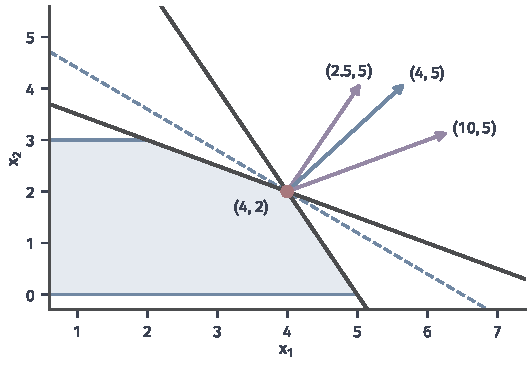
\includegraphics[width=90mm]{figures/05-optimization/01-linear-programming/matplotlib/simplex-cost-range/figure.pdf}
 \caption{产品一利润$p_1$的有效范围。深灰粗线是过$(4,2)$的两条活动约束，蓝色虚线是当前利润$p_1=4$的等值线。三支箭头只表示方向：蓝色是当前利润向量，紫色是范围端点$p_1=2.5$和$p_1=10$的利润向量，两者分别垂直于两条活动约束。}
 \label{fig:simplex-cost-range}
\end{BookInlineFigure}

表~\ref{tab:simplex-parameter-ranges}列出全部五个参数的结果。

\begin{BookInlineTable}
 \centering
 \begin{tabular}{cccl}
  \toprule
  参数 & 当前值 & 有效范围 & 变化率\\
  \midrule
  $b_1$ & $8$ & $[5,\ 9.5]$ & 利润$+2$\\
  $b_2$ & $10$ & $[7,\ 16]$ & 利润$+1$\\
  $b_3$ & $3$ & $[2,\ \infty)$ & 利润不变\\
  $p_1$ & $4$ & $[2.5,\ 10]$ & 利润$+x_1^\star=+4$\\
  $p_2$ & $5$ & $[2,\ 8]$ & 利润$+x_2^\star=+2$\\
  \bottomrule
 \end{tabular}
 \caption{单个参数变化时最优基$(1,5,2)$的有效范围，变化率指参数每增加一单位时最优利润的变化，只在范围内有效。}
 \label{tab:simplex-parameter-ranges}
\end{BookInlineTable}

几个参数同时变化时，结论要从向量形式读取。设右端变化$\Delta\bm{b}$，基$B$保持可行的条件是
\[
 \bar{\bm{x}}_B+\bm{A}_B^{-1}\Delta\bm{b}\geq\bm{0}.
\]
这是$\Delta\bm{b}$的一个多面体，不是逐个区间的乘积。把各个单独的范围同时用到极端，可能已经出界。

\paragraph{越出范围之后}
范围的端点不是答案的终点，只是这个基失效的位置。越过右端的范围，基失去原始可行性而保持对偶可行，这正是第~\ref{sec:simplex-dual}节的出发点。例如$b_1=11$时$x_5=-1$，对偶单纯形法一次换基就得到基$(1,3,2)$和解$(7/2,3)$，利润$29$，这与图~\ref{fig:simplex-rhs-range}(b)的平台一致。

越过目标系数的范围，基失去对偶可行性而保持原始可行，这时用原始单纯形法接着走。例如$p_1=12$时$s_3=-2/3$，$x_3$入基，$\bm{u}=(-1/3,-2/3,2/3)^\top$，比值检验给出$x_2$出基，点走到$(5,0)$，利润$60$。

把一个个基的有效范围拼起来，最优值就成为参数的分段线性函数，图~\ref{fig:simplex-rhs-range}(b)是一个例子，折点是换基发生的位置。在一般约束下，值函数和解映射如何随参数变化，由第~\ref{chap:parametric-sensitivity}章研究。

\section{最坏情形复杂度}
\label{sec:simplex-worst-case}

单纯形法有限终止，但有限不等于快。换基次数在最坏情况下能有多大，它和一次换基的代价是什么关系，实际表现又该怎样理解？

\paragraph{换基次数与每轮代价}
总运算量是两个因子的乘积：换基次数乘以每轮代价。第~\ref{sec:simplex-revised}节处理的是后者，稠密实现下每轮是$m$和$n$的低次多项式。本节讨论前者。基的个数最多是从$n$个下标中选$m$个的组合数，随规模指数增长，所以有限终止本身给不出多项式界。问题在于，算法会不会真的走那么多步。

\paragraph{Klee--Minty构造}
下面这族例子表明确实可能。第$n$个问题有$n$个变量和$n$个约束：
\begin{equation}
 \begin{aligned}
 \max\quad & z_n=\sum_{j=1}^n2^{n-j}x_j\\
 \text{s.t.}\quad & x_i+\sum_{j<i}2^{i-j+1}x_j\leq5^i,\quad i=1,\ldots,n,\\
 & \bm{x}\geq\bm{0}.
 \end{aligned}
 \label{eq:simplex-klee-minty}
\end{equation}
它属于Klee和Minty提出的压扁立方体构造\scite{math-klee1972simplex}。$n=2$时约束是$x_1\leq5$，$4x_1+x_2\leq25$，目标是$2x_1+x_2$。从原点出发，Dantzig规则选系数大的$x_1$，走到$(5,0)$；接着$x_2$入基，走到$(5,5)$；最后第一个松弛变量入基，走到$(0,25)$。四个顶点全被访问，如图~\ref{fig:simplex-klee-minty-plane}所示。

\begin{BookInlineFigure}
 \centering
 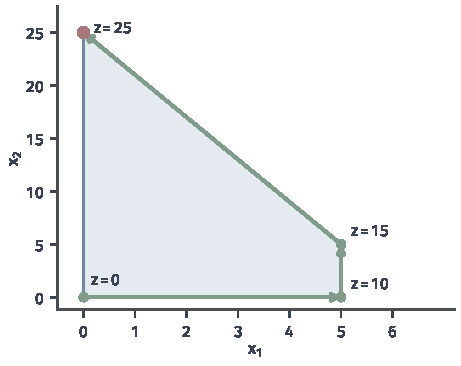
\includegraphics[width=78mm]{figures/05-optimization/01-linear-programming/matplotlib/simplex-klee-minty-plane/figure.pdf}
 \caption{$n=2$的Klee--Minty问题。可行域（浅蓝）有四个顶点，绿色路径依次访问全部四个，每个顶点旁标出目标值$z$，红点是最优解$(0,25)$。注意最优点其实与起点相邻，算法却绕了远路。}
 \label{fig:simplex-klee-minty-plane}
\end{BookInlineFigure}

$n=3$时情况相同，图~\ref{fig:simplex-klee-minty-cube}是可行域的示意。路径走完底面的四个顶点，上升一次，再把顶面的四个顶点反向走一遍。

\begin{BookInlineFigure}
 \centering
 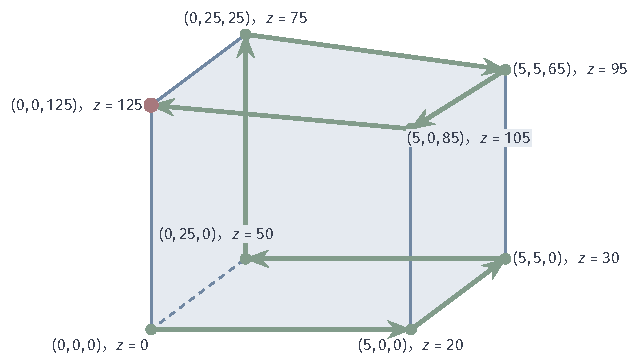
\includegraphics[width=108mm]{figures/05-optimization/01-linear-programming/tikz/simplex-klee-minty-cube/figure.pdf}
 \caption{$n=3$的Klee--Minty问题的示意，画成立方体，顶点坐标和目标值$z$是真实数据，比例不真实。绿色路径是Dantzig规则访问的顺序，共$7$次换基、走遍$8$个顶点，红点是最优解。}
 \label{fig:simplex-klee-minty-cube}
\end{BookInlineFigure}

这种“走完一面、再反着走一遍”的结构可以写成对$n$的归纳。为了写证明，先观察目标和约束之间的递推关系。记第$i$个松弛变量为$w_i$。由式~\eqref{eq:simplex-klee-minty}，第$n$个目标和第$n$个约束都可以用$z_{n-1}$表示：
\begin{equation}
 z_n=2z_{n-1}+x_n,\qquad w_n=5^n-x_n-4z_{n-1}.
 \label{eq:simplex-klee-minty-recursion}
\end{equation}
前$n-1$个约束恰好是第$n-1$个问题的约束，其中不含$x_n$和$w_n$。

下面用“字典”的语言：字典是把基变量和目标写成非基变量函数的表达式，也就是式~\eqref{eq:simplex-basic-form}和式~\eqref{eq:simplex-objective-form}的另一种叫法。最大化时，Dantzig规则选目标表达式中系数最大的正系数变量入基，这与最小化标准型中选最负的$s_j$是同一条规则。

\begin{theorem}[Klee--Minty问题的换基次数]
 \label{thm:simplex-klee-minty}
 对问题~\eqref{eq:simplex-klee-minty}，从全部松弛变量组成的基出发，Dantzig规则恰好经过$2^n-1$次换基到达最优解，最优值为$5^n$。
\end{theorem}

\begin{proof}
 对$n$归纳证明一个更强的命题。把从全松弛基出发、最大化$z_n$的运行称为上行，记为$U_n$；把从$U_n$的终点出发、最大化$-z_n$的运行称为下行，记为$D_n$。命题是：$U_n$和$D_n$各有$2^n-1$次换基；$U_n$过程中$z_n$从$0$增加到$5^n$，$D_n$过程中$z_n$从$5^n$减少到$0$并回到全松弛基；所有字典的目标系数都是整数。

 $n=1$时$z_1=x_1$，$w_1=5-x_1$。上行时$x_1$入基，一次换基后$z_1=5-w_1$。下行时目标是$-z_1=-5+w_1$，$w_1$入基，一次换基后$-z_1=-x_1$。命题成立。

 设命题对$n-1$成立，先看$U_n$。由式~\eqref{eq:simplex-klee-minty-recursion}，它分三段。

 第一段。设第$n-1$个问题的字典中$z_{n-1}$的系数为$d_k$，它们是整数。此时$z_n$的系数是$2d_k$，而$x_n$的系数是$1$。只要有$d_k>0$，就有$2d_k\geq2>1$，Dantzig规则的选择与$U_{n-1}$完全相同。第$n$行也不起限制作用，因为$x_n=0$且$z_{n-1}\leq5^{n-1}$，由式~\eqref{eq:simplex-klee-minty-recursion}得
 \[
  w_n\geq5^n-4\cdot5^{n-1}=5^{n-1}>0.
 \]
 所以算法照搬$U_{n-1}$，$2^{n-1}-1$次换基后$z_{n-1}=5^{n-1}$，所有$d_k\leq0$。

 第二段。此时只有$x_n$的系数为正，它入基。$x_n$只出现在第$n$行，所以$w_n$出基，$x_n=5^{n-1}$。这是一次换基。把$x_n=5^n-w_n-4z_{n-1}$代入$z_n$，目标变为
 \[
  z_n=5^n-w_n-2z_{n-1}.
 \]

 第三段。现在$w_n$的系数是$-1$，其余系数是$-2d_k$，后者正是$D_{n-1}$的目标$-z_{n-1}$放大$2$倍，$w_n$的系数为负，不会入基。第$n$行现在是$x_n=5^n-w_n-4z_{n-1}$，$w_n=0$时$x_n\geq5^{n-1}>0$，不起限制作用。所以算法照搬$D_{n-1}$，$2^{n-1}-1$次换基后$z_{n-1}=0$，所有系数非正，算法停止，此时$z_n=5^n$。

 三段合计$2(2^{n-1}-1)+1=2^n-1$次换基。

 再看$D_n$，它从$-z_n=-5^n+w_n+2z_{n-1}$开始，$z_{n-1}$的字典是全松弛基。第一段中$w_n$的系数是$1$，其余是$2d_k$，同样的比较说明算法照搬$U_{n-1}$，第$n$行$x_n\geq5^{n-1}>0$不起限制作用。第二段只有$w_n$的系数为正，它入基，$x_n$出基，代入后目标变为
 \[
  -z_n=-x_n-2z_{n-1}.
 \]
 第三段照搬$D_{n-1}$，第$n$行$w_n\geq5^{n-1}>0$不起限制作用，最后回到全松弛基，$z_n=0$。

 整数性由式~\eqref{eq:simplex-klee-minty-recursion}的递推保持，因为各段目标都是归纳假设中的整数系数乘$\pm2$再加上系数为$\pm1$的$x_n$或$w_n$。归纳完成。
\end{proof}

证明的要点在于系数的差距：前$n-1$个变量的系数翻倍，所以只要还有事可做，Dantzig规则就不会理会$x_n$；右端$5^i$的快速增长保证第$n$行不起限制作用。换一种规则结论就可能改变，图~\ref{fig:simplex-klee-minty-counts}(a)中Bland规则在这族例子上的步数少一些，但这只说明这族例子不是专门针对Bland规则构造的，其他构造同样能使Bland规则走指数多步。是否存在一条换基规则能保证多项式次换基，至今没有答案。

\begin{BookInlineFigure}
 \centering
 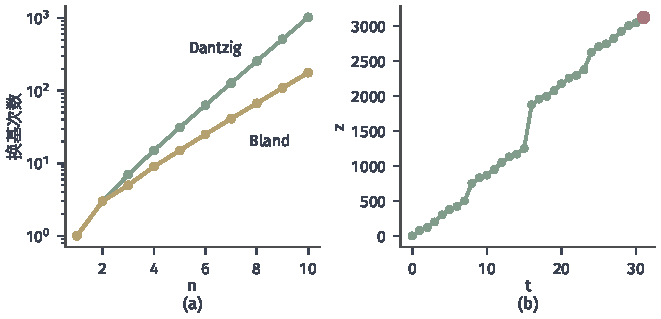
\includegraphics[width=112mm]{figures/05-optimization/01-linear-programming/matplotlib/simplex-klee-minty-counts/figure.pdf}
 \caption{Klee--Minty问题的实测结果，精确有理数运算。(a)~换基次数随$n$变化，纵轴取对数；绿线是Dantzig规则，恰为$2^n-1$；黄线是Bland规则。(b)~$n=5$时Dantzig规则各步的目标值，共$31$步，红点是最优值$3125$。}
 \label{fig:simplex-klee-minty-counts}
\end{BookInlineFigure}

\paragraph{最坏情形与实际表现}
定理~\ref{thm:simplex-klee-minty}是对一族特殊问题的结论，并不刻画算法在一般问题上的行为。长期的实践表明，单纯形法在大多数实际问题上的换基次数远小于组合数，常是约束数的不大的倍数。

图~\ref{fig:simplex-random-pivots}是一个小实验：$\bm{A},\bm{c}$的元素在$(0,1)$上独立均匀抽取，$\bm{b}=\bm{1}$，$m=n$，每种规模取$30$个随机种子。平均换基次数随规模温和增长，$m=320$时约$655$次，比Klee--Minty问题的指数增长慢得多。

\begin{BookInlineFigure}
 \centering
 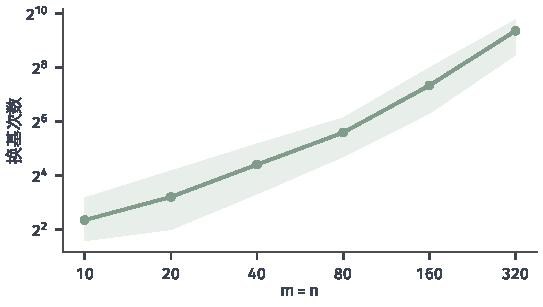
\includegraphics[width=92mm]{figures/05-optimization/01-linear-programming/matplotlib/simplex-random-pivots/figure.pdf}
 \caption{一种随机模型上Dantzig规则的换基次数，两轴都是对数刻度。绿线是$30$个随机种子的平均值，浅绿色带是最小值到最大值的范围。实验条件：$m=n$，$\bm{A},\bm{c}$的元素在$(0,1)$上独立均匀，$\bm{b}=\bm{1}$，起始基是全松弛基。}
 \label{fig:simplex-random-pivots}
\end{BookInlineFigure}

这个实验只说明这一随机模型上的情况，不能外推成对任意问题的保证。实际问题带有特定的结构，有时比随机模型容易，有时因退化严重而困难得多。理论上也有在特定随机扰动模型下给出多项式期望步数的结果，那些结论依赖扰动模型，并不告诉我们某一个具体实例要走多少步。

所以这里的两个判断要分开说：最坏情形下，Dantzig规则的换基次数可以随维数指数增长，这是定理；实际问题上换基次数通常不大，这是经验观察，没有无条件的平均复杂度保证。这个差别也是下一章研究多项式时间方法的原因之一。

\section{本章小结}
\label{sec:simplex-summary}

本章开头的问题是怎样在有限但极多的顶点之间找到最优的一个。单纯形法的回答是：用基来表示顶点，用约化成本判断哪条边值得走，用比值检验决定走多远，用对偶候选写出最优性证书。工厂的例子经过三次换基，从$(0,0)$走到$(4,2)$，并得到资源的对偶价格$(2,1,0)$。

算法的每个环节都有明确的条件。起步需要可行基，没有时用人工变量，两阶段法或符号化的大M法把它们排除；有限的$M$要超过对偶价格，这一点事先并不知道。退化基使步长为零，同一点对应多个基，循环可能发生，Bland规则或字典序规则在精确算术下保证有限终止。实现上修正单纯形法只维护基矩阵的因子，浮点运算要求小心选主元、定期重新分解，并在结束时重新核查。

算法的结果总是带着证据，表~\ref{tab:simplex-outcomes}汇总了三种停止结果。

\begin{BookInlineTable}
 \centering
 \begin{tabular}{lll}
  \toprule
  结果 & 检验 & 证据\\
  \midrule
  最优 & 可行基上$\bm{s}\geq\bm{0}$ & 原始解和对偶解，目标相等\\
  无界 & $s_q<0$且$\bm{u}\leq\bm{0}$ & 可行点和方向$\bm{d}$，$\bm{c}^\top\bm{d}<0$\\
  不可行 & 第一阶段$\phi^\star>0$，& $\bm{y}$，满足$\bm{A}^\top\bm{y}\leq\bm{0}$，$\bm{b}^\top\bm{y}>0$\\
  & 或对偶单纯形法无候选 & （后者取$\bm{y}=-\bm{\rho}$）\\
  \bottomrule
 \end{tabular}
 \caption{单纯形法的三种停止结果及其证据。}
 \label{tab:simplex-outcomes}
\end{BookInlineTable}

得到最优基以后，还能继续使用它。基的可行性和最优性分别管着右端和目标系数，固定基的参数分析读出每个参数的有效范围和影子价格；越出范围后，右端的变化交给对偶单纯形法，目标系数的变化交给原始单纯形法，只需少量换基。这种复用是单纯形法在整数规划等反复求解场合的重要优势。

有限终止不等于快。Klee--Minty构造说明Dantzig规则的换基次数最坏可以指数增长，实践中换基次数虽然通常不大，却没有无条件的理论保证。第~\ref{chap:lp-interior-point}章将研究另一条路线：不沿边界走，而从可行域内部逼近最优解。


\chapter{内点法}
\label{chap:lp-interior-point}

第~\ref{chap:simplex-method}章的工厂问题里，单纯形法从原点出发，沿可行域的边走过几个顶点，到达最优顶点$(4,2)$。每到一个顶点，都要决定下一步走哪条边。顶点的数目可以随维数指数增长，第~\ref{chap:simplex-method}章末尾的构造说明，这种逐个顶点的走法在最坏情形下确实可能走遍它们。于是有一个自然的问题：能不能不贴着边走，而从可行域的中间穿过去？

穿过中间要解决三件事。一是在内部靠什么指路：内部的每个点都可行，目标又是线性的，梯度处处相同，单看目标看不出该往哪里停。二是怎样防止撞上边界，同时又让终点能落在边界上，因为线性规划的最优解总在边界上。三是走到什么程度算完：内部的点永远不会恰好是顶点，“差不多最优”要有能核对的含义。

本章的回答是第~\ref{chap:linear-programming}章对偶理论的一个直接延伸。把互补松弛条件$x_is_i=0$放宽成$x_is_i=\mu$，再让正数$\mu$逐渐减小到零，方程组的解就连成一条从内部通向最优面的光滑曲线。第一节建立这条曲线，第二节用Newton法沿它前进，并在一个能手算的小例子上逐轮写出全部计算。

后面四节处理算法落地时的问题。起点从哪里来，放在第三节；三项残差怎样决定停止、近似解怎样变成基和严格证书，放在第四节；第五节证明一种路径跟踪规则的迭代次数只随$\sqrt{n}$增长，并说明这和线性规划的多项式可解性是什么关系；最后一节在工厂问题上把内点法和单纯形法放在一起比较。一般非线性约束上的内点法由第~\ref{chap:nonlinear-interior-point}章讨论。

\section{中心路径}
\label{sec:lpipm-central-path}

在可行域内部，沿怎样一条路线走，才能既不撞上边界，又最终到达最优解？答案是一条由对偶理论确定的曲线。我们先回顾要用到的对偶事实，再从一维的障碍函数讲起。

\paragraph{标准型与对偶}
本章讨论第~\ref{chap:linear-programming}章的标准型线性规划及其对偶：
\begin{equation}
 \min_{\bm{x}}\ \bm{c}^\top\bm{x}\quad\text{s.t.}\quad\bm{A}\bm{x}=\bm{b},\quad\bm{x}\geq\bm{0},
 \label{eq:lpipm-primal}
\end{equation}
\begin{equation}
 \max_{\bm{y},\bm{s}}\ \bm{b}^\top\bm{y}\quad\text{s.t.}\quad\bm{A}^\top\bm{y}+\bm{s}=\bm{c},\quad\bm{s}\geq\bm{0},
 \label{eq:lpipm-dual}
\end{equation}
其中$\bm{A}\in\mathbb{R}^{m\times n}$满行秩，$\bm{y}\in\mathbb{R}^m$无符号限制，$\bm{s}\in\mathbb{R}^n$称为对偶松弛。两个最优值分别记为$p^\star$和$d^\star$。

那一章的两个结论是本章的出发点。第一个是目标差的恒等式：若$\bm{x}$原始可行，$(\bm{y},\bm{s})$对偶可行，把$\bm{c}=\bm{A}^\top\bm{y}+\bm{s}$和$\bm{b}=\bm{A}\bm{x}$代入目标差，得到
\begin{equation}
 \bm{c}^\top\bm{x}-\bm{b}^\top\bm{y}
 =(\bm{A}^\top\bm{y}+\bm{s})^\top\bm{x}-(\bm{A}\bm{x})^\top\bm{y}
 =\bm{x}^\top\bm{s}.
 \label{eq:lpipm-gap-identity}
\end{equation}
左边称为对偶间隙。因为$\bm{x},\bm{s}\geq\bm{0}$，它非负，这就是弱对偶。

第二个是强对偶：问题可行且最优值有限时，$p^\star=d^\star$。于是$(\bm{x},\bm{y},\bm{s})$最优，当且仅当它同时满足
\begin{equation}
 \bm{A}\bm{x}=\bm{b},\qquad\bm{A}^\top\bm{y}+\bm{s}=\bm{c},\qquad x_is_i=0\ (i=1,\ldots,n),\qquad\bm{x},\bm{s}\geq\bm{0}.
 \label{eq:lpipm-kkt}
\end{equation}
中间的条件是互补松弛。前两组方程是线性的，难处全在$x_is_i=0$：对每个下标，要决定是$x_i$为零还是$s_i$为零。这是一个组合选择，单纯形法用基来做这个选择，一次换基改动一个下标。

全章贯穿下面这个小例子，只有一条等式约束：
\begin{equation}
 \min_{\bm{x}}\ x_1+2x_2+3x_3\quad\text{s.t.}\quad x_1+x_2+x_3=1,\quad\bm{x}\geq\bm{0}.
 \label{eq:lpipm-running}
\end{equation}
这里$n=3$，$m=1$，$\bm{A}=[1\ 1\ 1]$，$b=1$，$\bm{c}=(1,2,3)^\top$。可行集是$\mathbb{R}^3$中以三个单位向量为顶点的三角形。

对偶约束是$y+s_i=c_i$，即$\bm{s}=(1-y,\,2-y,\,3-y)^\top$，$\bm{s}\geq\bm{0}$等价于$y\leq1$，对偶目标就是$y$本身。最优解和最优对偶解都一眼可得：
\[
 \bm{x}^\star=(1,0,0)^\top,\qquad y^\star=1,\qquad\bm{s}^\star=(0,1,2)^\top,\qquad p^\star=d^\star=1.
\]
可以核对$x_i^\star s_i^\star$全为零。

\paragraph{贴边走与穿过去}
图~\ref{fig:lpipm-edge-vs-interior}是第~\ref{chap:simplex-method}章的工厂问题。黄线是单纯形法的路线，它贴着边界，在三个拐角上各做了一次选择。绿线是本节要建立的路径，它从内部一个点出发，平滑地弯向最优顶点，途中不需要决定任何“走哪条边”的问题。

可以把可行域想成一间房间，最优解在墙角。贴墙走，每到拐角都要判断往哪边转；从房间中央穿过去，没有拐角，但需要两样东西：一种不让人撞墙的力，以及一种随时间减弱这个力的办法，否则永远到不了墙角。这个比喻在终点处失效：真正的解就在墙上，所以排斥力必须在极限中消失，下面的$\mu\downarrow0$就是这件事。

\begin{BookInlineFigure}
  \centering
  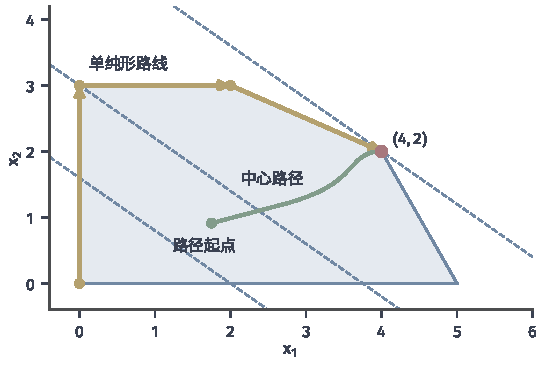
\includegraphics[width=92mm]{figures/05-optimization/01-linear-programming/matplotlib/lpipm-edge-vs-interior/figure.pdf}
  \caption{工厂问题的两条路线。浅蓝区域是可行域，蓝色虚线是利润的等值线，红点是最优顶点$(4,2)$。黄线是单纯形法经过的顶点序列$(0,0)$、$(0,3)$、$(2,3)$、$(4,2)$；绿线是中心路径，从$\mu$很大时的内部点出发，随$\mu$减小弯向最优顶点，全程不碰边界。}
  \label{fig:lpipm-edge-vs-interior}
\end{BookInlineFigure}

\paragraph{一维的障碍}
先看最简单的情形：在$x\geq0$上最小化$f(x)=x$，解是边界点$x=0$。在目标上加一项$-\mu\log x$，其中$\mu>0$，它在$x\downarrow0$时趋于$+\infty$，像一堵逐渐升高的墙，把迭代挡在$x>0$的一侧。这时要解的是
\[
 \min_{x>0}\ x-\mu\log x.
\]
令导数$1-\mu/x$为零，得到唯一的最小点
\[
 x=\mu.
\]
图~\ref{fig:lpipm-log-barrier}显示了两件事。图(a)中，$\mu$越小，墙贴得越紧，离墙稍远的地方几乎不受影响。图(b)中，绿点是加了障碍后的最小点，它随$\mu$减小沿$x=\mu$滑向真正的解$x=0$。

\begin{BookInlineFigure}
  \centering
  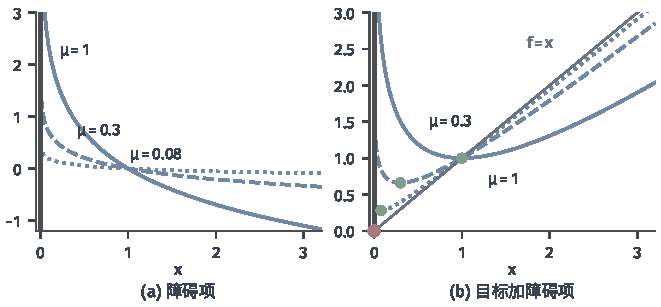
\includegraphics[width=112mm]{figures/05-optimization/01-linear-programming/matplotlib/lpipm-log-barrier/figure.pdf}
  \caption{一维的对数障碍。(a)障碍项$-\mu\log x$，实线、虚线、点线分别对应$\mu=1,0.3,0.08$，深灰粗线是边界$x=0$。(b)目标$f(x)=x$（细灰线）加上障碍项后的三条曲线，绿点是各自的最小点$x=\mu$，红点是真正的解$x=0$。}
  \label{fig:lpipm-log-barrier}
\end{BookInlineFigure}

\paragraph{对数障碍问题}
回到问题~\eqref{eq:lpipm-primal}，对每个坐标都加一项障碍。这里要留意“内部”的含义。例~\eqref{eq:lpipm-running}的可行集是$\mathbb{R}^3$中的一块三角形，厚度为零，没有通常意义下的内点。障碍只负责不等式$\bm{x}\geq\bm{0}$，等式$\bm{A}\bm{x}=\bm{b}$始终严格保持，所以内部是相对等式约束而言的，指满足等式且所有分量为正的点。

\begin{definition}[严格可行]
\label{def:lpipm-strictly-feasible}
满足$\bm{A}\bm{x}=\bm{b}$且$\bm{x}>\bm{0}$的点称为原始\term{严格可行}（strictly feasible）点。满足$\bm{A}^\top\bm{y}+\bm{s}=\bm{c}$且$\bm{s}>\bm{0}$的$(\bm{y},\bm{s})$称为对偶严格可行点。两者都存在时，记
\begin{equation}
 \mathcal{F}^{\circ}=\bigl\{(\bm{x},\bm{y},\bm{s}):\bm{A}\bm{x}=\bm{b},\ \bm{A}^\top\bm{y}+\bm{s}=\bm{c},\ \bm{x}>\bm{0},\ \bm{s}>\bm{0}\bigr\}.
 \label{eq:lpipm-strict-set}
\end{equation}
\end{definition}

严格可行点不一定存在。约束$x_1+x_2=0$、$\bm{x}\geq\bm{0}$的可行集只有原点，其中没有正的点。例~\eqref{eq:lpipm-running}中，$\bm{x}=(1/3,1/3,1/3)^\top$与$y=0$、$\bm{s}=(1,2,3)^\top$都严格可行。

对$\mu>0$，定义\term{对数障碍}（logarithmic barrier）问题
\begin{equation}
 \min_{\bm{x}}\ B_\mu(\bm{x})=\bm{c}^\top\bm{x}-\mu\sum_{i=1}^n\log x_i
 \quad\text{s.t.}\quad\bm{A}\bm{x}=\bm{b},\quad\bm{x}>\bm{0}.
 \label{eq:lpipm-barrier}
\end{equation}
图~\ref{fig:lpipm-bowls}画出例~\eqref{eq:lpipm-running}中$B_\mu$的等值线。线性目标本身没有碗底，障碍项在三条边上竖起墙，围出一个碗。$\mu$大时碗底靠近三角形中央，$\mu$小时墙贴向边界，碗底被线性目标推向最优顶点。

\begin{BookInlineFigure}
  \centering
  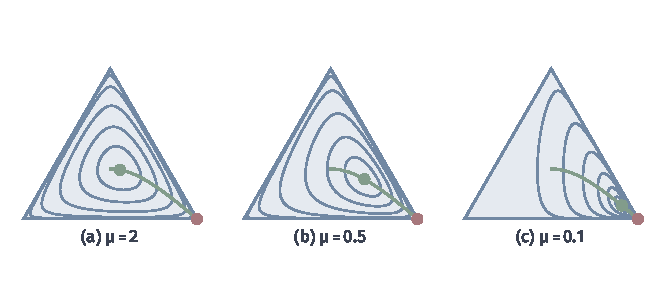
\includegraphics[width=112mm]{figures/05-optimization/01-linear-programming/matplotlib/lpipm-bowls/figure.pdf}
  \caption{例~\eqref{eq:lpipm-running}的障碍目标$B_\mu$在三角形上的等值线（蓝线）。绿线是全部碗底连成的曲线，绿点是当前$\mu$的碗底，红点是最优顶点。$\mu$减小时，碗底沿绿线向红点移动，碗也越来越贴近边界。}
  \label{fig:lpipm-bowls}
\end{BookInlineFigure}

\paragraph{一阶条件给出扰动的互补}
$B_\mu$的梯度是$\bm{c}-\mu\bm{X}^{-1}\bm{1}$，其中$\bm{X}=\operatorname{diag}(\bm{x})$，$\bm{1}$是全一向量。在仿射集合$\{\bm{x}:\bm{A}\bm{x}=\bm{b}\}$上，能移动的方向是$\bm{A}$的零空间，一阶条件要求梯度与零空间正交。$\bm{A}$的零空间的正交补是$\bm{A}^\top$的列空间，所以一阶条件是：存在$\bm{y}$使
\[
 \bm{c}-\mu\bm{X}^{-1}\bm{1}=\bm{A}^\top\bm{y}.
\]

这里出现了一个与$\bm{c}-\bm{A}^\top\bm{y}$相等的正向量，正是对偶松弛的样子。令$\bm{s}=\mu\bm{X}^{-1}\bm{1}$，上式成为$\bm{A}^\top\bm{y}+\bm{s}=\bm{c}$，而$\bm{s}$的定义就是$x_is_i=\mu$。三组条件合起来是
\begin{equation}
 \bm{A}\bm{x}=\bm{b},\qquad\bm{A}^\top\bm{y}+\bm{s}=\bm{c},\qquad x_is_i=\mu\ (i=1,\ldots,n),\qquad\bm{x},\bm{s}>\bm{0}.
 \label{eq:lpipm-central}
\end{equation}
把它与最优性条件~\eqref{eq:lpipm-kkt}逐项对比，只有互补松弛一处不同：$x_is_i=0$换成了$x_is_i=\mu$。

图~\ref{fig:lpipm-complementarity-corner}说明这个改动的好处。在$(x_i,s_i)$平面上，$x_is_i=0$、$x_i,s_i\geq0$是一个直角折线，组合选择就是选落在哪条腿上。把它换成双曲线$x_is_i=\mu$，折角被磨圆了，曲线是光滑的，可以用微积分处理；$\mu$越小，曲线越贴近折角。

\begin{BookInlineFigure}
  \centering
  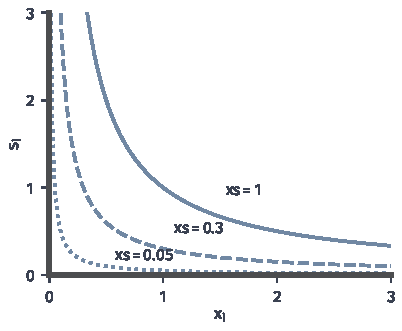
\includegraphics[width=68mm]{figures/05-optimization/01-linear-programming/matplotlib/lpipm-complementarity-corner/figure.pdf}
  \caption{互补条件的光滑化。深灰粗线是$x_is_i=0$、$x_i,s_i\geq0$的直角折线，蓝色曲线是$x_is_i=\mu$，实线、虚线、点线分别对应$\mu=1,0.3,0.05$。$\mu\downarrow0$时曲线贴近折线，但对每个正的$\mu$，$x_i$和$s_i$都严格为正。}
  \label{fig:lpipm-complementarity-corner}
\end{BookInlineFigure}

\paragraph{存在唯一的条件}
碗底并不总是存在，下面的定理说明它需要原始和对偶两侧都有严格可行点。

\begin{theorem}[中心点的存在唯一]
\label{thm:lpipm-central-exists}
设$\bm{A}$满行秩，$\mu>0$。方程组~\eqref{eq:lpipm-central}有解，当且仅当$\mathcal{F}^{\circ}$非空。此时解$(\bm{x}(\mu),\bm{y}(\mu),\bm{s}(\mu))$唯一，且$\bm{x}(\mu)$是障碍问题~\eqref{eq:lpipm-barrier}的唯一最小点。
\end{theorem}

\begin{proof}
必要性：方程组的解本身就是$\mathcal{F}^{\circ}$中的点。

充分性分两步。先证最小点存在。取$(\bar{\bm{y}},\bar{\bm{s}})$对偶严格可行，在原始可行点上，由$\bm{c}=\bm{A}^\top\bar{\bm{y}}+\bar{\bm{s}}$和$\bm{A}\bm{x}=\bm{b}$，目标可以改写为
\[
 \bm{c}^\top\bm{x}=\bm{b}^\top\bar{\bm{y}}+\bar{\bm{s}}^\top\bm{x},
\]
于是
\[
 B_\mu(\bm{x})=\bm{b}^\top\bar{\bm{y}}+\sum_{i=1}^n\bigl(\bar{s}_ix_i-\mu\log x_i\bigr).
\]
因为$\bar{s}_i>0$，每个一元函数$\bar{s}_it-\mu\log t$在$(0,\infty)$上有下界，并且在$t\downarrow0$和$t\to\infty$时都趋于$+\infty$。

于是对原始严格可行点$\bm{x}^{(0)}$，考虑下水平集
\[
 \bigl\{\bm{x}:\bm{A}\bm{x}=\bm{b},\ \bm{x}>\bm{0},\ B_\mu(\bm{x})\leq B_\mu(\bm{x}^{(0)})\bigr\}.
\]
其中每个坐标都落在某个区间$[\epsilon,R]$内，$\epsilon>0$，这是非空紧集。连续函数在紧集上取到最小值，这就是障碍问题的一个最小点。

再证一阶条件与最小点等价，并得到唯一性。最小点在相对内部，一阶条件成立，于是得到方程组~\eqref{eq:lpipm-central}的一个解。反过来，设$(\bm{x},\bm{y},\bm{s})$是一个解。函数$-\log t$是凸函数，所以$B_\mu$在可行集上是严格凸的，对任何可行的$\bm{x}'$有
\[
 B_\mu(\bm{x}')\geq B_\mu(\bm{x})+\nabla B_\mu(\bm{x})^\top(\bm{x}'-\bm{x})=B_\mu(\bm{x})+\bm{y}^\top\bm{A}(\bm{x}'-\bm{x})=B_\mu(\bm{x}),
\]
这说明$\bm{x}$是最小点。严格凸性保证最小点唯一，于是$\bm{x}$唯一，$\bm{s}=\mu\bm{X}^{-1}\bm{1}$也唯一。$\bm{A}^\top$列满秩，$\bm{A}^\top\bm{y}=\bm{c}-\bm{s}$给出唯一的$\bm{y}$。
\end{proof}

对偶严格可行这个条件不能省。问题$\min 0$、$x_1-x_2=0$、$\bm{x}\geq\bm{0}$有原始严格可行点$(1,1)$，最优值为$0$。它的障碍目标在可行射线$x_1=x_2=r$上等于$-2\mu\log r$，当$r\to\infty$时趋于$-\infty$，没有最小点。原因在对偶一侧：对偶约束$y+s_1=0$、$-y+s_2=0$迫使$s_1+s_2=0$，严格可行点不存在。

\begin{definition}[中心路径]
\label{def:lpipm-central-path}
当$\mathcal{F}^{\circ}$非空时，$\mu$取遍$(0,\infty)$，方程组~\eqref{eq:lpipm-central}的解构成一条曲线
\begin{equation}
 \mathcal{C}=\bigl\{(\bm{x}(\mu),\bm{y}(\mu),\bm{s}(\mu)):\mu>0\bigr\},
 \label{eq:lpipm-central-path}
\end{equation}
称为\term{中心路径}（central path）。其中的点称为中心点。
\end{definition}

这个名字可以这样理解：方程组要求所有乘积$x_is_i$相等，没有哪个坐标比别的坐标更靠近自己的边界，点保持在“中央”。下面的例子把路径完整地写出来。

\begin{example}[贯穿例的中心路径]
\label{ex:lpipm-central-closed-form}
在问题~\eqref{eq:lpipm-running}中，$s_i=c_i-y$，$x_is_i=\mu$给出$x_i=\mu/(c_i-y)$。代入$x_1+x_2+x_3=1$，消去$\bm{x}$，得到$\mu$与$y$的关系
\[
 \mu=\Bigl(\frac{1}{1-y}+\frac{1}{2-y}+\frac{1}{3-y}\Bigr)^{-1},\qquad y<1.
\]
所以路径可以用$y$作参数直接写出。

取$y=0$，则$\bm{s}=(1,2,3)^\top$，括号内是$1+\tfrac12+\tfrac13=\tfrac{11}{6}$，于是
\[
 \mu=\frac{6}{11},\qquad\bm{x}=\Bigl(\frac{6}{11},\frac{3}{11},\frac{2}{11}\Bigr)^\top.
\]
三个乘积都等于$6/11$，三个分量之和为$1$。

再取$y=1/2$，则$\bm{s}=(\tfrac12,\tfrac32,\tfrac52)^\top$，括号内是$2+\tfrac23+\tfrac25=\tfrac{46}{15}$，于是
\[
 \mu=\frac{15}{46},\qquad\bm{x}=\Bigl(\frac{15}{23},\frac{5}{23},\frac{3}{23}\Bigr)^\top.
\]

两端的行为也能读出来。$y\to-\infty$时$\mu\to\infty$，$x_i$趋于相等，极限是$(1/3,1/3,1/3)^\top$。$y\uparrow1$时第一项发散，$\mu\to0$，$\bm{x}\to(1,0,0)^\top$。
\end{example}

图~\ref{fig:lpipm-central-path}把这条路径画在三角形上。起点是$\mu\to\infty$的极限，这一点最大化$\sum_i\log x_i$，称为可行集的\term{解析中心}（analytic center）。解析中心只有在可行集有界时才存在，它只由约束决定，与目标无关；目标$\bm{c}$的作用是决定路径离开中心后朝哪里弯。

\begin{BookInlineFigure}
  \centering
  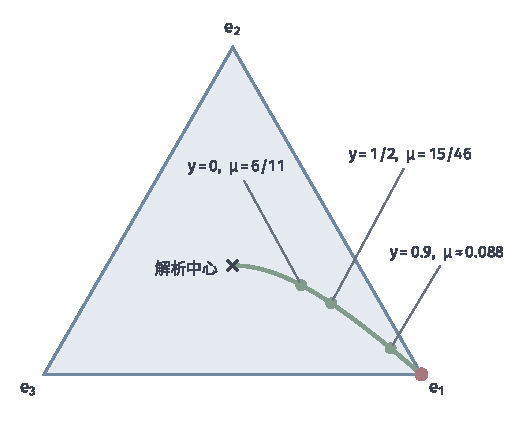
\includegraphics[width=90mm]{figures/05-optimization/01-linear-programming/matplotlib/lpipm-central-path/figure.pdf}
  \caption{贯穿例的中心路径。三角形是可行集，三个角是单位向量，黑叉是解析中心$(1/3,1/3,1/3)^\top$，绿线是中心路径，绿点是例~\ref{ex:lpipm-central-closed-form}算出的中心点以及$y=0.9$的中心点，红点是最优顶点$\bm{e}_1$。}
  \label{fig:lpipm-central-path}
\end{BookInlineFigure}

\paragraph{间隙恰好是$n\mu$}
中心路径最有用的性质是，沿路径的对偶间隙可以直接读出来。中心点原始、对偶都可行，把式~\eqref{eq:lpipm-gap-identity}用到这里，再代入$x_is_i=\mu$，得到
\begin{equation}
 \bm{c}^\top\bm{x}(\mu)-\bm{b}^\top\bm{y}(\mu)=\sum_{i=1}^nx_i(\mu)s_i(\mu)=n\mu.
 \label{eq:lpipm-central-gap}
\end{equation}

它把“还差多远”变成了一个已知的数。由弱对偶$\bm{b}^\top\bm{y}(\mu)\leq p^\star$，原始目标误差不超过间隙：
\begin{equation}
 \bm{c}^\top\bm{x}(\mu)-p^\star\leq n\mu.
 \label{eq:lpipm-central-error}
\end{equation}
要让误差不超过$\varepsilon$，走到$\mu\leq\varepsilon/n$就够了。在例~\ref{ex:lpipm-central-closed-form}中，$y=0$的中心点目标值是$6/11+6/11+6/11=18/11$，对偶目标是$0$，间隙$18/11$正好等于$3\mu$。

这个结论用到了精确的中心点。迭代算法只能走到中心路径附近，这时间隙怎样计算，第~\ref{sec:lpipm-accuracy}节会逐项说明。

\paragraph{路径的终点}
式~\eqref{eq:lpipm-central-gap}说明目标值收敛到最优值，却没有说点本身收敛到哪里。解不唯一时，这个问题的答案并不平凡。先看例子：把目标换成$c=(0,0,1)$，约束不变，此时第三个分量为零的整条边都是最优解。

这时$\bm{s}=(-y,-y,1-y)$，记$r=-y>0$，则$x_1=x_2=\mu/r$，$x_3=\mu/(1+r)$，等式约束给出
\[
 \frac{2\mu}{r}+\frac{\mu}{1+r}=1.
\]
令$\mu\downarrow0$，第二项趋于零，第一项必须趋于$1$，所以$r\approx2\mu$，$x_1=x_2=\mu/r\to1/2$。路径的极限是$(1/2,1/2,0)^\top$，它不是顶点，而是最优边的中点，如图~\ref{fig:lpipm-optimal-face}(b)所示。

\begin{BookInlineFigure}
  \centering
  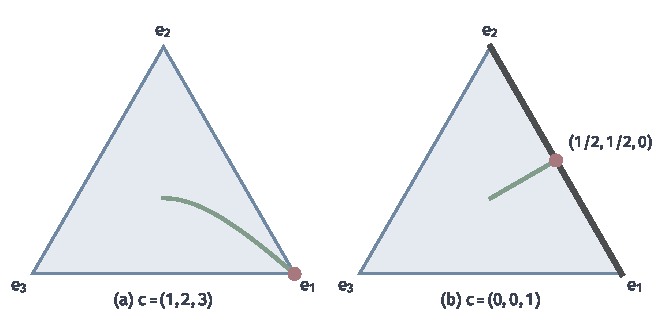
\includegraphics[width=112mm]{figures/05-optimization/01-linear-programming/matplotlib/lpipm-optimal-face/figure.pdf}
  \caption{路径的极限由最优解集决定。绿线是中心路径。(a)$\bm{c}=(1,2,3)$，最优解唯一，路径通向顶点$\bm{e}_1$（红点）。(b)$\bm{c}=(0,0,1)$，最优解集是深灰粗线表示的整条边，路径通向这条边的中点$(1/2,1/2,0)^\top$，这是最优面上的解析中心，不是顶点。}
  \label{fig:lpipm-optimal-face}
\end{BookInlineFigure}

一般情形的结论如下。设最优解集合为$\bm{S}_{\mathrm{P}}$，这是可行集的一个面，称为\term{最优面}（optimal face）。若某对原始、对偶最优解满足对每个下标$x_i^\star+s_i^\star>0$，就称这对解是\term{严格互补}（strictly complementary）的。下面的定理说，中心路径收敛到一对严格互补的解，并且在最优面上取在“最中央”的位置。

\begin{theorem}[中心路径的极限]
\label{thm:lpipm-central-limit}
设$\bm{A}$满行秩，$\mathcal{F}^{\circ}$非空。当$\mu\downarrow0$时，$(\bm{x}(\mu),\bm{y}(\mu),\bm{s}(\mu))$收敛到一对最优解$(\hat{\bm{x}},\hat{\bm{y}},\hat{\bm{s}})$。记$B=\{i:\hat{x}_i>0\}$，$N=\{i:\hat{s}_i>0\}$，则$B$与$N$互不相交且并集为$\{1,\ldots,n\}$，并且$\hat{\bm{x}}$是最优面上使下式最大的唯一点：
\begin{equation}
 \sum_{i\in B}\log x_i.
 \label{eq:lpipm-face-center}
\end{equation}
\end{theorem}

\begin{proof}
关键工具是一个正交关系。设$\bm{x},\bm{x}'$都满足等式$\bm{A}\bm{x}=\bm{b}$，$(\bm{y},\bm{s}),(\bm{y}',\bm{s}')$都满足$\bm{A}^\top\bm{y}+\bm{s}=\bm{c}$。则$\bm{x}-\bm{x}'$属于$\bm{A}$的零空间，$\bm{s}-\bm{s}'=-\bm{A}^\top(\bm{y}-\bm{y}')$属于$\bm{A}^\top$的列空间，于是
\begin{equation}
 (\bm{x}-\bm{x}')^\top(\bm{s}-\bm{s}')=0.
 \label{eq:lpipm-orthogonality}
\end{equation}

\emph{有界性。}取固定的$(\bar{\bm{x}},\bar{\bm{y}},\bar{\bm{s}})\in\mathcal{F}^{\circ}$。把式~\eqref{eq:lpipm-orthogonality}用到中心点和这一点，展开并用$\bm{x}(\mu)^\top\bm{s}(\mu)=n\mu$，得到
\[
 \bar{\bm{s}}^\top\bm{x}(\mu)+\bar{\bm{x}}^\top\bm{s}(\mu)=n\mu+\bar{\bm{x}}^\top\bar{\bm{s}}.
\]
左边各项非负且$\bar{\bm{x}},\bar{\bm{s}}>\bm{0}$，所以$\mu\in(0,1]$时$\bm{x}(\mu)$、$\bm{s}(\mu)$有界。$\bm{A}^\top$列满秩，$\bm{y}(\mu)$也有界。

\emph{聚点是最优解。}取$\mu_k\downarrow0$使三元组收敛到一个聚点$(\hat{\bm{x}},\hat{\bm{y}},\hat{\bm{s}})$。它满足两组等式，$\hat{\bm{x}},\hat{\bm{s}}\geq\bm{0}$，且由式~\eqref{eq:lpipm-central-gap}，$\hat{\bm{x}}^\top\hat{\bm{s}}=0$，所以是最优解。

\emph{一个归一化的恒等式。}设$(\bm{x}^\star,\bm{y}^\star,\bm{s}^\star)$是任意一对最优解，由互补松弛，它们的内积为零。把式~\eqref{eq:lpipm-orthogonality}用到中心点和这一对最优解，得到
\[
 (\bm{s}^\star)^\top\bm{x}(\mu)+(\bm{x}^\star)^\top\bm{s}(\mu)=n\mu.
\]
两边除以$\mu$，用$x_i(\mu)/\mu=1/s_i(\mu)$和$s_i(\mu)/\mu=1/x_i(\mu)$，得到
\begin{equation}
 \sum_{i=1}^n\frac{s_i^\star}{s_i(\mu)}+\sum_{i=1}^n\frac{x_i^\star}{x_i(\mu)}=n.
 \label{eq:lpipm-normalized}
\end{equation}

\emph{严格互补。}式~\eqref{eq:lpipm-normalized}左边每一项非负，所以$x_i(\mu)\geq x_i^\star/n$。令$\mu=\mu_k\to0$，得$\hat{x}_i\geq x_i^\star/n$，即每个最优解的正分量也是$\hat{\bm{x}}$的正分量；对$\hat{\bm{s}}$同理。

再把聚点$(\hat{\bm{x}},\hat{\bm{s}})$本身当作最优解代入式~\eqref{eq:lpipm-normalized}，令$\mu_k\to0$。$i\in B$时$\hat{x}_i/x_i(\mu_k)\to1$，$i\in N$时$\hat{s}_i/s_i(\mu_k)\to1$，其余项为零，于是
\[
 \lvert B\rvert+\lvert N\rvert=n.
\]
互补性$\hat{\bm{x}}^\top\hat{\bm{s}}=0$说明$B\cap N=\varnothing$，所以它们的并集是全部下标。

\emph{极限唯一。}由上一步，任何聚点的正分量位置都包含任何最优解的正分量位置，所以所有聚点有相同的$B$和$N$，任何原始最优解在$N$上为零。在式~\eqref{eq:lpipm-normalized}中取$\bm{s}^\star=\hat{\bm{s}}$、$\bm{x}^\star$为任意原始最优解，令$\mu_k\to0$，得到
\[
 \lvert N\rvert+\sum_{i\in B}\frac{x_i^\star}{\hat{x}_i}=n,\qquad\text{即}\qquad\sum_{i\in B}\frac{x_i^\star-\hat{x}_i}{\hat{x}_i}=0.
\]
这正是凹函数~\eqref{eq:lpipm-face-center}在$\hat{\bm{x}}$处沿任意最优面方向的方向导数为零，所以$\hat{\bm{x}}$是它在最优面上的最大点。严格凹性保证最大点唯一，因此所有聚点的$\bm{x}$部分相同。对$\hat{\bm{s}}$同理，得到相应的$\sum_{i\in N}\log s_i$最大的唯一点，再由$\bm{A}^\top$列满秩，$\hat{\bm{y}}$也唯一。有界序列只有一个聚点，所以收敛。
\end{proof}

这个定理有两个直接的推论。最优解唯一时，路径通向顶点；最优解不唯一时，路径通向最优面的相对内部，得不到顶点。此外，定理顺带证明了线性规划在$\mathcal{F}^{\circ}$非空时总有严格互补解。

这里的下标集$B$和单纯形法的基不是一回事：$B$是极限点的正分量位置，可以多于或少于$m$个。内点法最终告诉我们的是“哪些变量为正”，而不是直接给出一个基，第~\ref{sec:lpipm-accuracy}节会处理两者的转换。

\section{原始—对偶路径跟踪}
\label{sec:lpipm-path-following}

上一节得到一条曲线，但求曲线上的一个点要解一组非线性方程。于是要问：不把每个中心点算准，怎样一步步沿曲线走向$\mu=0$？做法是把三组条件当作一个方程组，同时更新$\bm{x},\bm{y},\bm{s}$。

\paragraph{主要思想：对扰动方程作Newton线性化}
当前点记为$(\bm{x},\bm{y},\bm{s})$，只要求$\bm{x},\bm{s}>\bm{0}$。为了同时适用下一节的不可行起点，这里不假设它满足等式约束。当前的平均互补量是
\begin{equation}
 \mu=\frac{\bm{x}^\top\bm{s}}{n}.
 \label{eq:lpipm-mu}
\end{equation}

我们不把目标定为$\mu=0$，而定为路径上$\sigma\mu$处的中心点，其中$\sigma\in[0,1]$称为\term{中心化参数}（centering parameter）。这一轮想达到的是
\[
 \bm{A}\bm{x}=\bm{b},\qquad\bm{A}^\top\bm{y}+\bm{s}=\bm{c},\qquad x_is_i=\sigma\mu.
\]

把新的点写成$\bm{x}+\Delta\bm{x}$、$\bm{y}+\Delta\bm{y}$、$\bm{s}+\Delta\bm{s}$，代入这三组方程。前两组本身就是线性的，第三组展开是
\[
 x_is_i+s_i\Delta x_i+x_i\Delta s_i+\Delta x_i\Delta s_i=\sigma\mu.
\]
唯一的非线性项是$\Delta x_i\Delta s_i$，它是两个小量的乘积。Newton法的做法就是把它丢掉，留下关于方向的线性方程组。

为了写得紧凑，定义三个残差，分别度量原始等式、对偶等式和互补目标还差多少：
\begin{equation}
 \bm{r}_{\mathrm{p}}=\bm{A}\bm{x}-\bm{b},\qquad
 \bm{r}_{\mathrm{d}}=\bm{A}^\top\bm{y}+\bm{s}-\bm{c},\qquad
 \bm{r}_{\mathrm{c}}=\sigma\mu\bm{1}-\bm{X}\bm{S}\bm{1},
 \label{eq:lpipm-residuals}
\end{equation}
其中$\bm{S}=\operatorname{diag}(\bm{s})$。这样，方向$(\Delta\bm{x},\Delta\bm{y},\Delta\bm{s})$由下面的线性方程组确定：
\begin{equation}
 \begin{bmatrix}
 \bm{A}&\bm{0}&\bm{0}\\
 \bm{0}&\bm{A}^\top&\bm{I}\\
 \bm{S}&\bm{0}&\bm{X}
 \end{bmatrix}
 \begin{bmatrix}\Delta\bm{x}\\\Delta\bm{y}\\\Delta\bm{s}\end{bmatrix}
 =
 \begin{bmatrix}-\bm{r}_{\mathrm{p}}\\-\bm{r}_{\mathrm{d}}\\\bm{r}_{\mathrm{c}}\end{bmatrix}.
 \label{eq:lpipm-newton}
\end{equation}
第一行要求走完之后原始残差消失，第二行要求对偶残差消失，第三行要求所有乘积都变成$\sigma\mu$。系数矩阵正是三组方程关于$(\bm{x},\bm{y},\bm{s})$的Jacobian矩阵。

\paragraph{为什么线性化$x_is_i=\mu$，而不是$s_i=\mu/x_i$}
两种写法定义同一条曲线，线性化后的方程却差别很大。图~\ref{fig:lpipm-newton-bilinear}取一个坐标，固定$s=1$、$\mu=1$，方程的根是$x=1$。图(a)对$\mu/x-s=0$作Newton法，从$x=2.4$出发，切线与横轴的交点落在$x\approx-0.96$，越过了边界。

这件事不是偶然的。$1/x$在$x$大时很平，切线斜率过小，步子迈得过大；具体地，这个迭代是$x\mapsto x(2-x)$，$x>2$时一步变成负数。图(b)对$xs-\mu=0$作Newton法，函数本身关于$x$是直线，一步到根。一般情形中$s$也在变，方程对两个变量合起来是双线性的，但误差只是一个二阶小项$\Delta x_i\Delta s_i$，线性模型“可信的范围”比倒数形式大得多。

\begin{BookInlineFigure}
  \centering
  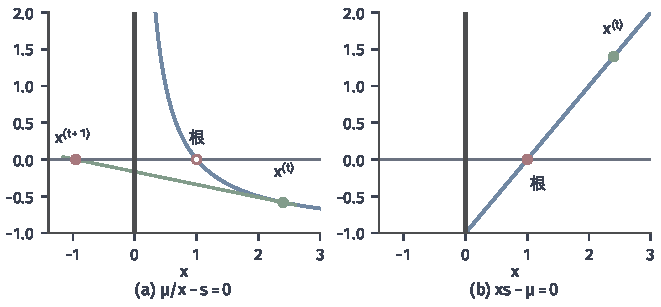
\includegraphics[width=112mm]{figures/05-optimization/01-linear-programming/matplotlib/lpipm-newton-bilinear/figure.pdf}
  \caption{同一条约束的两种写法，$s=\mu=1$，根都是$x=1$（红圈或红点）。(a)蓝线是$\mu/x-s$，绿线是在$x^{(t)}=2.4$处的切线，Newton步落到$x^{(t+1)}\approx-0.96$（红点），越过边界（深灰粗线）。(b)蓝线是$xs-\mu$，本身就是直线，Newton步一步到根。}
  \label{fig:lpipm-newton-bilinear}
\end{BookInlineFigure}

\paragraph{消元：把方程组化成一个$m\times m$的问题}
方程组~\eqref{eq:lpipm-newton}的大小是$2n+m$，但结构很特殊，可以依次消元。由第二行，
\begin{equation}
 \Delta\bm{s}=-\bm{r}_{\mathrm{d}}-\bm{A}^\top\Delta\bm{y}.
 \label{eq:lpipm-ds}
\end{equation}
第三行是$\bm{S}$与$\bm{X}$两个对角矩阵分别作用在两个方向上，直接解出
\begin{equation}
 \Delta\bm{x}=\bm{S}^{-1}\bigl(\bm{r}_{\mathrm{c}}-\bm{X}\Delta\bm{s}\bigr).
 \label{eq:lpipm-dx}
\end{equation}
把式~\eqref{eq:lpipm-ds}代入式~\eqref{eq:lpipm-dx}，得到
\[
 \Delta\bm{x}=\bm{S}^{-1}\bigl(\bm{r}_{\mathrm{c}}+\bm{X}\bm{r}_{\mathrm{d}}\bigr)+\bm{S}^{-1}\bm{X}\bm{A}^\top\Delta\bm{y}.
\]

记对角矩阵$\bm{D}=\bm{X}\bm{S}^{-1}$，它的对角元是$x_i/s_i$。把上式代入第一行$\bm{A}\Delta\bm{x}=-\bm{r}_{\mathrm{p}}$，就得到只含$\Delta\bm{y}$的方程。定义
\begin{equation}
 \bm{M}=\bm{A}\bm{D}\bm{A}^\top,\qquad
 \bm{h}=-\bm{r}_{\mathrm{p}}-\bm{A}\bm{S}^{-1}\bigl(\bm{r}_{\mathrm{c}}+\bm{X}\bm{r}_{\mathrm{d}}\bigr),
 \label{eq:lpipm-normal-data}
\end{equation}
方向$\Delta\bm{y}$由下式给出：
\begin{equation}
 \Delta\bm{y}=\bm{M}^{-1}\bm{h}.
 \label{eq:lpipm-dy}
\end{equation}
$\bm{M}\Delta\bm{y}=\bm{h}$称为\term{正规方程}（normal equations），实际计算中用Cholesky分解求解，不显式求逆。求出$\Delta\bm{y}$后，由式~\eqref{eq:lpipm-ds}得到$\Delta\bm{s}$，再由式~\eqref{eq:lpipm-dx}得到$\Delta\bm{x}$。

这一步之所以总能进行，靠的是下面的事实。

\begin{lemma}[Newton方程可解]
\label{lem:lpipm-newton-solvable}
设$\bm{A}$满行秩，$\bm{x},\bm{s}>\bm{0}$。则$\bm{M}=\bm{A}\bm{D}\bm{A}^\top$对称正定，方程组~\eqref{eq:lpipm-newton}有唯一解，由式~\eqref{eq:lpipm-dy}、\eqref{eq:lpipm-ds}、\eqref{eq:lpipm-dx}给出。
\end{lemma}

\begin{proof}
$\bm{D}$的对角元全为正。对任何$\bm{v}\neq\bm{0}$，$\bm{A}$满行秩给出$\bm{A}^\top\bm{v}\neq\bm{0}$，于是
\[
 \bm{v}^\top\bm{M}\bm{v}=(\bm{A}^\top\bm{v})^\top\bm{D}(\bm{A}^\top\bm{v})>0,
\]
所以$\bm{M}$正定。上面的消元每一步都是等价变形，故方程组的解恰好由这三个公式给出。
\end{proof}

\paragraph{一步之后三个残差怎样变}
设步长为$\alpha\in(0,1]$，$\bm{x}^+=\bm{x}+\alpha\Delta\bm{x}$，$\bm{y}^+$、$\bm{s}^+$同理。前两组方程是线性的，把第一行、第二行代入，新的残差就是
\begin{equation}
 \bm{r}_{\mathrm{p}}^+=(1-\alpha)\bm{r}_{\mathrm{p}},\qquad\bm{r}_{\mathrm{d}}^+=(1-\alpha)\bm{r}_{\mathrm{d}}.
 \label{eq:lpipm-residual-update}
\end{equation}
走完单位步（$\alpha=1$）时，等式残差恰好为零，此后一直为零。

互补量的变化由展开式得到。把$\bm{x}^+$、$\bm{s}^+$代入内积，一次项由第三行给出
\[
 \bm{s}^\top\Delta\bm{x}+\bm{x}^\top\Delta\bm{s}=\bm{1}^\top\bm{r}_{\mathrm{c}}=n\sigma\mu-n\mu,
\]
于是
\begin{equation}
 (\bm{x}^+)^\top\bm{s}^+=\bigl(1-\alpha(1-\sigma)\bigr)\bm{x}^\top\bm{s}+\alpha^2\,\Delta\bm{x}^\top\Delta\bm{s}.
 \label{eq:lpipm-comp-update}
\end{equation}
当前点严格可行时，两个等式残差为零，第一行和第二行给出
\[
 \bm{A}\Delta\bm{x}=\bm{0},\qquad\Delta\bm{s}=-\bm{A}^\top\Delta\bm{y}.
\]
所以$\Delta\bm{x}^\top\Delta\bm{s}=0$，互补量精确地按因子$1-\alpha(1-\sigma)$下降。

\paragraph{步长：到边界的比例}
Newton方向可能把某个分量推成负数，所以步长要受限。沿方向走时，每个正分量到零的距离是确定的。定义能保持非负的最大步长
\begin{equation}
 \alpha_{\max}=\min\Bigl\{\min_{\Delta x_i<0}\frac{x_i}{-\Delta x_i},\ \min_{\Delta s_i<0}\frac{s_i}{-\Delta s_i}\Bigr\},
 \label{eq:lpipm-alpha-max}
\end{equation}
没有负分量时约定$\alpha_{\max}=+\infty$。这个量和单纯形法的比值检验是同一种计算，只是后者走到恰好有一个变量为零，这里不能走到那么远，否则下一轮的$\bm{S}^{-1}$或$\bm{D}$不存在。

取一个略小于$1$的比例$\eta$，例如$0.9$或$0.995$，令
\begin{equation}
 \alpha=\min\{1,\ \eta\,\alpha_{\max}\},
 \label{eq:lpipm-alpha}
\end{equation}
这称为\term{到边界的比例规则}（fraction-to-the-boundary rule）。图~\ref{fig:lpipm-step-rule}是贯穿例第一轮的情形：六个坐标沿方向变化，其中$s_1$最先降到零，$\alpha_{\max}$由它决定。

\begin{BookInlineFigure}
  \centering
  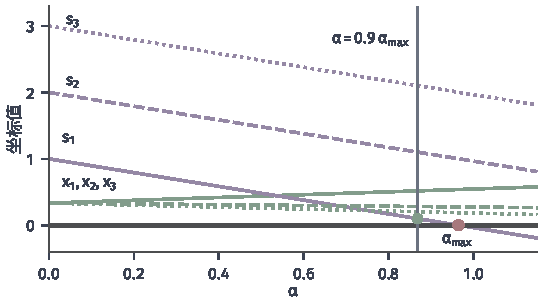
\includegraphics[width=92mm]{figures/05-optimization/01-linear-programming/matplotlib/lpipm-step-rule/figure.pdf}
  \caption{贯穿例第一轮各坐标沿Newton方向的变化，$\sigma=0.3$。紫线是$s_1,s_2,s_3$，绿线是$x_1,x_2,x_3$，实线、虚线、点线依次对应下标$1,2,3$，深灰粗线是边界。$s_1$在$\alpha_{\max}=55/57\approx0.965$处最先到达零（红点），取$\eta=0.9$后实际步长$\alpha=33/38\approx0.868$（竖线与绿点）。}
  \label{fig:lpipm-step-rule}
\end{BookInlineFigure}

\paragraph{中心化：两种力量的折中}
参数$\sigma$控制这一轮更想做什么。$\sigma=1$时目标是当前$\mu$处的中心点，方向只把点拉回路径，互补量不减；$\sigma=0$时目标直接是$\mu=0$，这个方向称为\term{仿射尺度方向}（affine-scaling direction），只求减小互补量，不管中心性。

可以把中心路径想成山谷的谷线，互补量是海拔。$\sigma=0$相当于只顾朝谷底方向走，容易撞上谷壁，步长被迫很小。$\sigma=1$相当于退回谷线，位置好了，海拔没降。合适的$\sigma$介于两者之间，类比的失效之处是，这里“谷壁”是$x_i$或$s_i$接近零的边界，不是某个目标函数的等高线。

\paragraph{计算过程}
下面把每一轮写成具体步骤，并在例~\eqref{eq:lpipm-running}上逐轮计算。取固定的中心化参数$\sigma=0.3$、比例$\eta=0.9$，容差$\varepsilon=10^{-3}$，起点选严格可行点。

\needspace{6\baselineskip}
\paragraph{变量}
\begin{itemize}
 \item $\bm{x}\in\mathbb{R}^n$：当前原始点，所有分量为正。
 \item $\bm{y}\in\mathbb{R}^m$：当前对偶变量。
 \item $\bm{s}\in\mathbb{R}^n$：当前对偶松弛，所有分量为正。
 \item $\mu$：当前平均互补量，由式~\eqref{eq:lpipm-mu}计算。
 \item $\bm{r}_{\mathrm{p}},\bm{r}_{\mathrm{d}},\bm{r}_{\mathrm{c}}$：式~\eqref{eq:lpipm-residuals}的三个残差，形状分别是$m$、$n$、$n$维。
 \item $\bm{D}$、$\bm{M}$、$\bm{h}$：对角缩放矩阵、$m\times m$的正规矩阵和右端，由式~\eqref{eq:lpipm-normal-data}计算。
 \item $\Delta\bm{x},\Delta\bm{y},\Delta\bm{s}$：本轮的方向，$\alpha_{\max},\alpha$是最大步长和实际步长。
\end{itemize}

\paragraph{初始化}
取严格可行的起点$(\bm{x}^{(0)},\bm{y}^{(0)},\bm{s}^{(0)})\in\mathcal{F}^{\circ}$，令$t=0$；起点怎样得到由下一节回答。例中取
\[
 \bm{x}^{(0)}=\Bigl(\frac13,\frac13,\frac13\Bigr)^\top,\qquad y^{(0)}=0,\qquad\bm{s}^{(0)}=(1,2,3)^\top.
\]
它满足等式约束，但不是中心点：三个乘积分别是$1/3$、$2/3$、$1$。

\needspace{6\baselineskip}
\paragraph{每轮更新}
在第$t$轮，以$(\bm{x}^{(t)},\bm{y}^{(t)},\bm{s}^{(t)})$为当前点：
\begin{enumerate}
 \item \textbf{检查停止。}按式~\eqref{eq:lpipm-residuals}计算$\bm{r}_{\mathrm{p}}$、$\bm{r}_{\mathrm{d}}$，按式~\eqref{eq:lpipm-mu}计算$\mu^{(t)}$。若等式残差和互补量都不超过容差，停止并输出当前点。

 例中第一轮
 \[
  \mu^{(0)}=\frac13\Bigl(\frac13+\frac23+1\Bigr)=\frac23,\qquad\bm{x}^\top\bm{s}=2>\varepsilon,
 \]
 等式残差都是零，继续。

 \item \textbf{计算互补残差。}按式~\eqref{eq:lpipm-residuals}计算$\bm{r}_{\mathrm{c}}$，这里的$\mu$取$\mu^{(t)}$。

 例中第一轮$\sigma\mu^{(0)}=1/5$，
 \[
  \bm{r}_{\mathrm{c}}=\frac15\bm{1}-\Bigl(\frac13,\frac23,1\Bigr)^\top=\Bigl(-\frac{2}{15},-\frac{7}{15},-\frac45\Bigr)^\top.
 \]

 \item \textbf{形成并求解正规方程。}由式~\eqref{eq:lpipm-normal-data}计算$\bm{M}$和$\bm{h}$，由式~\eqref{eq:lpipm-dy}得到$\Delta\bm{y}$。

 例中$\bm{r}_{\mathrm{p}},\bm{r}_{\mathrm{d}}$为零，$\bm{D}$的对角元是$x_i/s_i$，$\bm{A}$是一行全一，所以$\bm{M}$和$\bm{h}$都是数。第一轮
 \[
  M=\frac13+\frac16+\frac19=\frac{11}{18},\qquad h=-\sum_{i=1}^3\frac{r_{\mathrm{c},i}}{s_i}=\frac{2}{15}+\frac{7}{30}+\frac{4}{15}=\frac{19}{30},
 \]
 于是
 \[
  \Delta y=\frac{19/30}{11/18}=\frac{57}{55}\approx1.0364.
 \]

 \item \textbf{回代方向。}由式~\eqref{eq:lpipm-ds}得到$\Delta\bm{s}$，由式~\eqref{eq:lpipm-dx}得到$\Delta\bm{x}$。

 例中第一轮$\Delta\bm{s}=-\Delta y\bm{1}$，$\Delta x_i=(r_{\mathrm{c},i}-x_i\Delta s_i)/s_i$，于是
 \[
  \Delta\bm{s}=-\frac{57}{55}\bm{1},\qquad
  \Delta\bm{x}=\Bigl(\frac{7}{33},-\frac{2}{33},-\frac{5}{33}\Bigr)^\top.
 \]
 三个$\Delta x_i$相加为零，这正是$\bm{A}\Delta\bm{x}=\bm{0}$。

 \item \textbf{确定步长。}由式~\eqref{eq:lpipm-alpha-max}、\eqref{eq:lpipm-alpha}计算$\alpha_{\max}$和$\alpha$。

 例中第一轮三个$s_i$的比值分别是$\tfrac{55}{57},\tfrac{110}{57},\tfrac{165}{57}$，$x_2,x_3$的比值分别是$\tfrac{11}{2},\tfrac{11}{5}$，最小的是$s_1$的比值，所以
 \[
  \alpha_{\max}=\frac{55}{57}\approx0.9649,\qquad\alpha=\frac{9}{10}\cdot\frac{55}{57}=\frac{33}{38}\approx0.8684.
 \]

 \item \textbf{更新。}令
 \begin{equation}
  \begin{aligned}
  \bm{x}^{(t+1)}&=\bm{x}^{(t)}+\alpha\Delta\bm{x},\\
  \bm{y}^{(t+1)}&=\bm{y}^{(t)}+\alpha\Delta\bm{y},\\
  \bm{s}^{(t+1)}&=\bm{s}^{(t)}+\alpha\Delta\bm{s},
  \end{aligned}
  \label{eq:lpipm-update}
 \end{equation}
 然后令$t\leftarrow t+1$，回到第1步。这里原始变量和对偶变量用同一个步长，式~\eqref{eq:lpipm-comp-update}的精确下降公式依赖这一点。

 例中第一轮
 \[
  \bm{x}^{(1)}=\Bigl(\frac{59}{114},\frac{16}{57},\frac{23}{114}\Bigr)^\top\approx(0.5175,0.2807,0.2018)^\top,
 \]
 对偶部分是
 \[
  y^{(1)}=\frac{9}{10},\qquad\bm{s}^{(1)}=\Bigl(\frac{1}{10},\frac{11}{10},\frac{21}{10}\Bigr)^\top.
 \]
 按式~\eqref{eq:lpipm-comp-update}，互补量应是
 \[
  \Bigl(1-\frac{33}{38}\cdot\frac{7}{10}\Bigr)\cdot2=\frac{149}{190}\approx0.7842.
 \]
 直接计算$\sum_ix_i^{(1)}s_i^{(1)}$也得到这个数。

 三个乘积这时是$(0.0518,0.3088,0.4237)$，差距比起点时大了，这一步以中心性为代价换来了较长的步子。
\end{enumerate}

例中第二轮的中间量如下。当前$\mu^{(1)}=0.2614$，$\sigma\mu^{(1)}=0.07842$，
\[
 \begin{gathered}
 \bm{r}_{\mathrm{c}}=(0.0267,-0.2304,-0.3453)^\top,\\
 \bm{D}=\operatorname{diag}(5.1754,0.2552,0.0961).
 \end{gathered}
\]
第一个分量已经被压低，$x_1s_1$小于目标$\sigma\mu$，所以$r_{\mathrm{c},1}$变成正的，这一轮要把它往上拉。

正规方程给出
\[
 M=5.5267,\qquad h=0.1072,\qquad\Delta y=0.0194.
\]
回代得到
\[
 \Delta\bm{s}=-0.0194\,\bm{1},\qquad\Delta\bm{x}=(0.3670,-0.2045,-0.1625)^\top.
\]

这一轮$\alpha_{\max}=1.2412$，$0.9\alpha_{\max}>1$，所以取$\alpha=1$，于是
\[
 \begin{gathered}
 \bm{x}^{(2)}=(0.8846,0.0762,0.0392)^\top,\qquad y^{(2)}=0.9194,\\
 \bm{s}^{(2)}=(0.0806,1.0806,2.0806)^\top.
 \end{gathered}
\]
互补量精确地变为$0.3\times0.7842=0.2353$。

此后每轮都取$\alpha=1$，互补量每轮乘以$0.3$。表~\ref{tab:lpipm-run}列出全部$7$轮的中间量。第$7$轮后互补量约为$5.7\times10^{-4}$，不超过$\varepsilon$，算法停止。

\begin{BookInlineTable}
  \centering
  \footnotesize
  \begin{tabular}{@{}ccccccccc@{}}
    \toprule
    $t$ & $x_1^{(t)}$ & $x_2^{(t)}$ & $y^{(t)}$ & $\mu^{(t)}$ & $M$ & $\Delta y$ & $\alpha_{\max}$ & $\alpha$\\
    \midrule
    0 & 0.3333 & 0.3333 & 0 & 0.6667 & 0.6111 & 1.0364 & 0.9649 & 0.8684\\
    1 & 0.5175 & 0.2807 & 0.9 & 0.2614 & 5.527 & 0.0194 & 1.2412 & 1\\
    2 & 0.8846 & 0.0762 & 0.9194 & 0.0784 & 11.06 & 0.0610 & 1.3210 & 1\\
    3 & 0.9615 & 0.0261 & 0.9804 & 0.0235 & 49.12 & 0.0128 & 1.3851 & 1\\
    4 & 0.9892 & 0.0073 & 0.9932 & 0.0071 & 146.0 & 0.0047 & 1.4179 & 1\\
    5 & 0.9968 & 0.0021 & 0.9979 & 0.0021 & 477.3 & 0.0015 & 1.4247 & 1\\
    6 & 0.9990 & 0.0006 & 0.9994 & 0.0006 & 1579 & 0.0004 & 1.4274 & 1\\
    7 & 0.9997 & 0.0002 & 0.9998 & 0.0002 & & & & \\
    \bottomrule
  \end{tabular}
  \caption{贯穿例的逐轮中间量，$\sigma=0.3$、$\eta=0.9$。$x_3^{(t)}=1-x_1^{(t)}-x_2^{(t)}$，$s_i^{(t)}=c_i-y^{(t)}$。第$t$行的$M,\Delta y,\alpha_{\max},\alpha$是从第$t$个点出发那一轮的量。}
  \label{tab:lpipm-run}
\end{BookInlineTable}

最终得到
\[
 \hat{\bm{x}}\approx(0.9997,0.0002,0.0001)^\top,\qquad\hat{y}\approx0.9998,
\]
互补量约$5.7\times10^{-4}$，目标值$\bm{c}^\top\hat{\bm{x}}\approx1.0004$。由于迭代全程可行，间隙就是互补量，目标误差不超过$5.7\times10^{-4}$。实际误差约$3.8\times10^{-4}$，确实在这个界内。这里的$\hat{\bm{x}}$不是顶点，第~\ref{sec:lpipm-accuracy}节讨论这一点的影响。

\begin{BookInlineFigure}
  \centering
  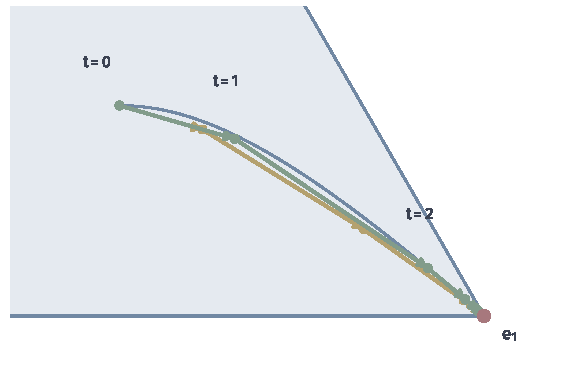
\includegraphics[width=96mm]{figures/05-optimization/01-linear-programming/matplotlib/lpipm-iterates/figure.pdf}
  \caption{贯穿例的迭代点，三角形局部放大。蓝线是中心路径，绿色是$\sigma=0.3$的路径跟踪，黄色是更激进的$\sigma=0.1$，红点是最优顶点$\bm{e}_1$。迭代点不在路径上，而是绕在路径附近前进。}
  \label{fig:lpipm-iterates}
\end{BookInlineFigure}

\paragraph{$\sigma$的取值}
图~\ref{fig:lpipm-iterates}中迭代点没有贴着路径，但始终在它附近。这种“附近”的程度可以用$\min_ix_is_i/\mu$度量，它等于$1$时点是中心点，接近$0$时某个乘积远低于平均。

图~\ref{fig:lpipm-sigma-tradeoff}比较了不同的$\sigma$。图(a)中，$\sigma$越小，互补量下降越快，但这只是因为每轮的目标更激进。图(b)说明了代价：$\sigma=0.1$前两轮的步长只有$0.63$和$0.68$，到$t=2$时中心性掉到$0.07$左右，靠后面的几轮才恢复。$\sigma=0.9$则一直很靠近中心，下降却极慢。

\begin{BookInlineFigure}
  \centering
  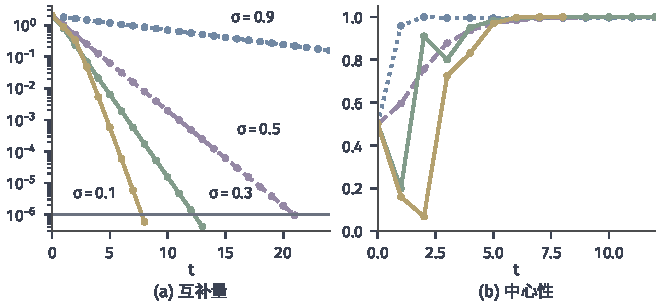
\includegraphics[width=112mm]{figures/05-optimization/01-linear-programming/matplotlib/lpipm-sigma-tradeoff/figure.pdf}
  \caption{中心化参数的影响，贯穿例，$\eta=0.9$。(a)互补量$\bm{x}^\top\bm{s}$随轮次的变化，灰色横线是$10^{-6}$。(b)中心性$\min_ix_is_i/\mu$，等于$1$表示恰好在中心路径上。绿线$\sigma=0.3$，黄线$\sigma=0.1$，紫色虚线$\sigma=0.5$，蓝色点线$\sigma=0.9$。}
  \label{fig:lpipm-sigma-tradeoff}
\end{BookInlineFigure}

\paragraph{预测—校正：先试走一步}
固定的$\sigma$有两个缺点：它不知道这一轮能走多远，也没有处理被丢掉的二阶项$\Delta x_i\Delta s_i$。\term{预测—校正}（predictor-corrector）方法用一次试算解决这两件事，额外代价只是多解一次已经分解好的方程组。

\emph{预测}是先解一次$\sigma=0$的方程组，得到仿射尺度方向$(\Delta\bm{x}^{\mathrm{a}},\Delta\bm{y}^{\mathrm{a}},\Delta\bm{s}^{\mathrm{a}})$，也就是令$\bm{r}_{\mathrm{c}}=-\bm{X}\bm{S}\bm{1}$。沿它能走的步长记为$\alpha^{\mathrm{a}}$，试走之后的平均互补量是
\begin{equation}
 \mu^{\mathrm{a}}=\frac{(\bm{x}+\alpha^{\mathrm{a}}\Delta\bm{x}^{\mathrm{a}})^\top(\bm{s}+\alpha^{\mathrm{a}}\Delta\bm{s}^{\mathrm{a}})}{n}.
 \label{eq:lpipm-mu-aff}
\end{equation}

这个数说明当前点有多好走：$\mu^{\mathrm{a}}$远小于$\mu$时，纯下降方向很有效，不需要多少中心化。常用的选法是
\begin{equation}
 \sigma=\Bigl(\frac{\mu^{\mathrm{a}}}{\mu}\Bigr)^3.
 \label{eq:lpipm-sigma-rule}
\end{equation}
三次方是一条经验规则，没有理论上的必然性。

\emph{校正}处理二阶项。式~\eqref{eq:lpipm-newton}假装$\Delta x_i\Delta s_i=0$，预测步已经给出了这一项的估计$\Delta x_i^{\mathrm{a}}\Delta s_i^{\mathrm{a}}$，于是把它移到右端：
\begin{equation}
 \bm{r}_{\mathrm{c}}=\sigma\mu\bm{1}-\bm{X}\bm{S}\bm{1}-\Delta\bm{X}^{\mathrm{a}}\Delta\bm{S}^{\mathrm{a}}\bm{1}.
 \label{eq:lpipm-corrector-rhs}
\end{equation}
用这个$\bm{r}_{\mathrm{c}}$按式~\eqref{eq:lpipm-normal-data}至\eqref{eq:lpipm-dx}求方向，步长仍按式~\eqref{eq:lpipm-alpha}。两次求解的系数矩阵$\bm{M}$相同，所以只分解一次，这一点在$\bm{M}$很大时决定了这个方法的价值。

例中第一轮，预测方向取$\sigma=0$，$M$与前面相同，右端变成$h=1$，得到
\[
 \Delta y^{\mathrm{a}}=\frac{18}{11},\qquad\Delta\bm{x}^{\mathrm{a}}=\Bigl(\frac{7}{33},-\frac{2}{33},-\frac{5}{33}\Bigr)^\top.
\]
这里$\Delta\bm{x}^{\mathrm{a}}$与固定$\sigma=0.3$时相同，是因为起点是三角形的解析中心，中心化分量在$\bm{x}$上恰好为零。

步长由$s_1$决定，试走后的互补量和中心化参数是
\[
 \alpha^{\mathrm{a}}=\frac{11}{18},\qquad\mu^{\mathrm{a}}=\frac{7}{27}\approx0.2593,\qquad\sigma=\Bigl(\frac{7}{18}\Bigr)^3\approx0.0588.
\]

校正的右端由式~\eqref{eq:lpipm-corrector-rhs}算出，其中$\sigma\mu\approx0.0392$，二阶项的估计是
\[
 \Delta\bm{X}^{\mathrm{a}}\Delta\bm{S}^{\mathrm{a}}\bm{1}\approx(-0.3471,0.0992,0.2479)^\top,
\]
于是
\[
 \bm{r}_{\mathrm{c}}\approx(0.0530,-0.7266,-1.2087)^\top,\qquad h\approx0.7132,\qquad\Delta y\approx1.1671.
\]

这一步的最大步长是$\alpha_{\max}\approx0.8568$，取$\alpha\approx0.7711$，得到
\[
 \bm{x}^{(1)}\approx(0.6742,0.2032,0.1226)^\top,\qquad y^{(1)}=0.9,\qquad\bm{x}^\top\bm{s}\approx0.5485.
\]
相比之下，固定$\sigma=0.3$第一轮后的互补量是$0.7842$。

图~\ref{fig:lpipm-predictor-corrector}(a)显示了校正的作用。黄色柱是单位预测步之后的乘积，第一个分量甚至为负，也就是说走完单位步会越界。绿色柱是校正后的单位步，三个乘积都向目标$\sigma\mu$靠拢，虽然这一轮离路径较远，并没有完全到位。

图(b)显示，整体上预测—校正用$7$轮把互补量降到$10^{-6}$以下，固定$\sigma=0.3$用$13$轮。需要说明，这是这个小例子上的观察，式~\eqref{eq:lpipm-sigma-rule}没有迭代次数的一般保证。

\begin{BookInlineFigure}
  \centering
  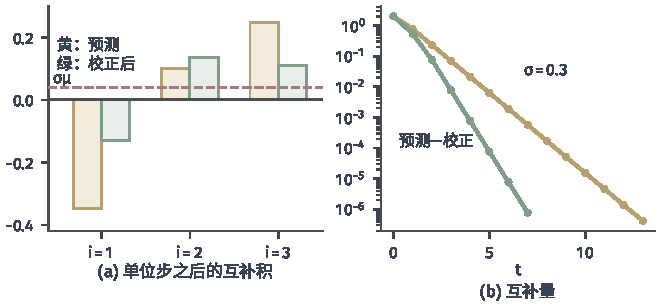
\includegraphics[width=112mm]{figures/05-optimization/01-linear-programming/matplotlib/lpipm-predictor-corrector/figure.pdf}
  \caption{预测—校正的效果，贯穿例。(a)从起点走单位步之后三个乘积$x_is_i$的值：黄色为预测方向，绿色为校正后方向，红色虚线是目标$\sigma\mu\approx0.039$。(b)互补量随轮次的变化，绿线为预测—校正，黄线为固定$\sigma=0.3$，两者都取$\eta=0.9$，容差为$10^{-6}$。}
  \label{fig:lpipm-predictor-corrector}
\end{BookInlineFigure}

\paragraph{计算代价}
每轮的主要工作是形成$\bm{M}=\bm{A}\bm{D}\bm{A}^\top$并作Cholesky分解。稠密情形下，形成$\bm{M}$需要约$m^2n$次运算，分解需要约$m^3/3$次运算；稀疏情形下取决于分解的填充，第~\ref{sec:lpipm-comparison}节再详细讨论。

$\bm{M}$的非零模式只由$\bm{A}$决定，每轮只有$\bm{D}$的数值在变，所以分解的符号结构只需分析一次。回代得到$\Delta\bm{s}$和$\Delta\bm{x}$的代价相对可以忽略。

\section{初始点}
\label{sec:lpipm-initial-point}

上一节的计算从一个严格可行点出发。贯穿例的约束很简单，这样的点一眼可见，一般问题却未必。接下来要弄清：起点从哪里来，起点不可行时算法还能不能用，问题本身没有严格可行点时又该怎么办？

\paragraph{可行初始方法}
最直接的想法是先求出一个严格可行点，再开始路径跟踪，这和单纯形法的第一阶段是同一个思路。对原始一侧，构造辅助问题
\begin{equation}
 \min_{\bm{x},\rho}\ \rho\quad\text{s.t.}\quad\bm{A}\bm{x}=\bm{b},\quad\bm{x}+\rho\bm{1}\geq\bm{0},\quad\rho\geq-1.
 \label{eq:lpipm-phase-one}
\end{equation}
$\rho$越小，$\bm{x}$离边界越有余量。下界$-1$只是为了防止$\rho$在可行集无界时下降到负无穷。

这个辅助问题的严格可行点是现成的：任取$\bm{A}\bm{x}=\bm{b}$的一个解，例如最小范数解$\bm{A}^\top(\bm{A}\bm{A}^\top)^{-1}\bm{b}$，再取足够大的$\rho$即可。最优值$\rho^\star$的符号给出三种结论：

\begin{itemize}
 \item $\rho^\star<0$：最优点满足$x_i\geq-\rho^\star>0$，这是原问题的严格可行点。
 \item $\rho^\star=0$：原问题可行，但没有严格可行点。
 \item $\rho^\star>0$：原问题不可行。
\end{itemize}

三种情形可以用同一个小例子看到。取两个变量和约束$x_1+x_2=a$。把两个分量约束相加，得到$a+2\rho\geq0$，即$\rho\geq-a/2$。取$a=1$时，$\rho^\star=-1/2$，最优点$(1/2,1/2)$严格可行。取$a=0$时，$\rho^\star=0$，可行点只有原点。取$a=-1$时，$\rho^\star=1/2$，原问题不可行。

这个方法有两点不足。辅助问题本身也是线性规划，且它的对偶一侧未必有严格可行点：只有不存在非零的$\bm{d}\geq\bm{0}$使$\bm{A}\bm{d}=\bm{0}$时才有，否则要先加上足够大的变量上界。另外，对偶一侧还要另解一个类似的问题，求出来的点也通常离中心路径很远，要用$\sigma$接近$1$的几步先作中心化。这些原因使大规模实现很少走这条路。

\paragraph{不可行初始方法}
更常用的做法是放弃“起点满足等式”这个要求，只保持$\bm{x},\bm{s}>\bm{0}$。方程组~\eqref{eq:lpipm-newton}的右端本来就含$\bm{r}_{\mathrm{p}}$和$\bm{r}_{\mathrm{d}}$，上一节的公式可以原样使用。式~\eqref{eq:lpipm-residual-update}说明，每走步长$\alpha$，两个等式残差都精确地乘以$1-\alpha$。

这和可行初始方法的区别在于，等式约束不再是“先满足的前提”，而是和互补量一起逐步降低的目标。迭代点在走向最优的同时走向可行。

用贯穿例试算，起点取$\bm{x}^{(0)}=\bm{s}^{(0)}=\bm{1}$、$y^{(0)}=0$，它不满足任何等式。残差是
\[
 r_{\mathrm{p}}=2,\qquad\bm{r}_{\mathrm{d}}=(0,-1,-2)^\top,\qquad\mu^{(0)}=1.
\]
取$\sigma=0.3$，$\bm{r}_{\mathrm{c}}=-0.7\,\bm{1}$。

由式~\eqref{eq:lpipm-normal-data}，$\bm{D}=\bm{I}$，于是
\[
 M=3,\qquad h=-2-\sum_{i=1}^3\bigl(r_{\mathrm{c},i}+r_{\mathrm{d},i}\bigr)=3.1,\qquad\Delta y=\frac{31}{30}\approx1.0333.
\]
回代得到
\[
 \Delta\bm{s}\approx(-1.0333,-0.0333,0.9667)^\top,\qquad\Delta\bm{x}\approx(0.3333,-0.6667,-1.6667)^\top.
\]

$\alpha_{\max}=0.6$由$x_3$决定，取$\alpha=0.54$。新的残差恰好是原来的$0.46$倍，点是
\[
 \bm{x}^{(1)}=(1.18,0.64,0.10)^\top,\qquad y^{(1)}=0.558,\qquad\bm{s}^{(1)}=(0.442,0.982,1.522)^\top.
\]
可以核对$r_{\mathrm{p}}=1.92-1=0.92=0.46\times2$。

接下来第二轮取$\alpha\approx0.894$，第三轮取到$\alpha=1$，等式残差降到舍入误差水平，此后成为可行迭代，如图~\ref{fig:lpipm-infeasible-start}(a)。

\begin{BookInlineFigure}
  \centering
  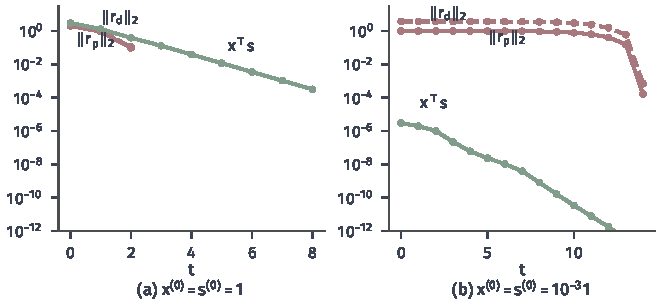
\includegraphics[width=112mm]{figures/05-optimization/01-linear-programming/matplotlib/lpipm-infeasible-start/figure.pdf}
  \caption{不可行起点的两种情况，贯穿例，$\sigma=0.3$、$\eta=0.9$，对数纵轴。红色实线是$\lVert\bm{r}_{\mathrm{p}}\rVert_2$，红色虚线是$\lVert\bm{r}_{\mathrm{d}}\rVert_2$，绿线是$\bm{x}^\top\bm{s}$。(a)起点$\bm{x}=\bm{s}=\bm{1}$，残差在第$3$轮取单位步后归零（图中不再画出）。(b)起点$\bm{x}=\bm{s}=10^{-3}\bm{1}$，互补量先极快地变小，而残差前十轮几乎不动，因为此间的步长只有$10^{-3}$到$10^{-1}$量级。}
  \label{fig:lpipm-infeasible-start}
\end{BookInlineFigure}

\paragraph{起点太小的后果}
图~\ref{fig:lpipm-infeasible-start}(b)把起点缩小到$10^{-3}\bm{1}$。这个起点的互补量已经小到$3\times10^{-6}$，等式残差却仍有$1$和$3.7$的量级。起点小，意味着方程$x_is_i\approx\sigma\mu$的线性化只允许很小的移动：Newton方向要消除大的等式残差，$\alpha_{\max}$却被很小的$x_i,s_i$限制，头几轮的步长只有约$7\times10^{-4}$。

算法最终还是走出来了，但这是这个例子的运气，不是一般保证。理论分析要求互补量不能比等式残差下降得快，常用的条件是
\begin{equation}
 \frac{\lVert(\bm{r}_{\mathrm{p}}^{(t)},\bm{r}_{\mathrm{d}}^{(t)})\rVert_2}{\mu^{(t)}}
 \leq C\,\frac{\lVert(\bm{r}_{\mathrm{p}}^{(0)},\bm{r}_{\mathrm{d}}^{(0)})\rVert_2}{\mu^{(0)}},
 \label{eq:lpipm-infeasible-ratio}
\end{equation}
其中$C\geq1$是常数，并且要求起点足够大。这种算法的全局收敛和复杂度结果需要较长的邻域分析，读者可查阅专著\scite{math-nocedal2006numerical}。在实现中，它对应的经验是起点的$\bm{x}$和$\bm{s}$要足够大，互补量相对残差不能太小。

\paragraph{一个常用的起点}
起点要兼顾两件事：接近满足等式，以及各分量足够大。一个常用的启发式分两步。先求最小范数意义下的近似：
\begin{equation}
 \tilde{\bm{x}}=\bm{A}^\top(\bm{A}\bm{A}^\top)^{-1}\bm{b},\qquad
 \tilde{\bm{y}}=(\bm{A}\bm{A}^\top)^{-1}\bm{A}\bm{c},\qquad
 \tilde{\bm{s}}=\bm{c}-\bm{A}^\top\tilde{\bm{y}}.
 \label{eq:lpipm-mehrotra-start}
\end{equation}
再把负分量和过小的分量整体平移成正的。贯穿例中$\bm{A}\bm{A}^\top=3$，于是$\tilde{\bm{x}}=\tfrac13\bm{1}$，$\tilde{y}=2$，$\tilde{\bm{s}}=(-1,0,1)^\top$。

平移分两步。第一步取$\delta_s=\max\{-1.5\min_i\tilde{s}_i,0\}=1.5$（$\tilde{\bm{x}}$已为正，$\delta_x=0$），得到$\hat{\bm{s}}=(0.5,1.5,2.5)^\top$。第二步按当前互补量再抬高一点，取
\[
 \hat{\delta}_x=\frac12\frac{\tilde{\bm{x}}^\top\hat{\bm{s}}}{\bm{1}^\top\hat{\bm{s}}}=\frac16,\qquad
 \hat{\delta}_s=\frac12\frac{\tilde{\bm{x}}^\top\hat{\bm{s}}}{\bm{1}^\top\tilde{\bm{x}}}=\frac34.
\]
最后的起点是
\[
 \bm{x}^{(0)}=\frac12\bm{1},\qquad y^{(0)}=2,\qquad\bm{s}^{(0)}=(1.25,2.25,3.25)^\top.
\]
这是一条经验规则，没有理论保证，但在实践中通常能避开图~\ref{fig:lpipm-infeasible-start}(b)的情形。

\paragraph{严格可行点不存在时}
定理~\ref{thm:lpipm-central-exists}说明，$\mathcal{F}^{\circ}$为空时中心路径不存在，路径跟踪失去了依据。这种情况有两类来源，处理方式不同。

一类来自建模的表述，问题本身可解。典型例子是把无符号变量写成两个非负变量之差$x=x^+-x^-$：两列互为相反数，第~\ref{sec:lpipm-central-path}节的反例已经说明，这样的问题对偶一侧没有严格可行点。又如约束$x_1+x_2=0$强迫两个变量恒为零。

\term{预处理}（presolve）承担这类任务：删去冗余的行以恢复满行秩，把被约束确定的变量代入，识别恒为零的变量，单独处理自由变量，并把行列缩放到相近的量级。预处理不改变最优解集（或给出恢复原解的办法），却能去掉一大批使严格可行性失效的结构。

另一类是问题真的不可行或无界。这时算法的迭代通常会发散，互补量和残差都下不去，但“没有收敛”不等于“证明了不可行”。我们需要一种方法，在问题不可解时也能输出一张可以核对的证书。

\paragraph{齐次自对偶嵌入}
思路是把原问题和对偶问题放进一个更大的、总有解的方程组里，用两个新的非负变量$\tau,\kappa$来判别结局。\term{齐次模型}（homogeneous model）是
\begin{equation}
 \begin{aligned}
 \bm{A}\bm{x}-\bm{b}\tau&=\bm{0},\\
 \bm{A}^\top\bm{y}+\bm{s}-\bm{c}\tau&=\bm{0},\\
 \bm{b}^\top\bm{y}-\bm{c}^\top\bm{x}-\kappa&=0,
 \end{aligned}
 \qquad\bm{x},\bm{s}\geq\bm{0},\quad\tau,\kappa\geq0.
 \label{eq:lpipm-homogeneous}
\end{equation}

零解总是满足它，所以这个模型不会没有解。不同的结局体现在非零解上：

\begin{itemize}
 \item $\tau>0$、$\kappa=0$：把$(\bm{x},\bm{y},\bm{s})$都除以$\tau$，前两行正是原始和对偶可行性，第三行说明目标相等，得到一对最优解。
 \item $\tau=0$、$\kappa>0$：此时$\bm{A}\bm{x}=\bm{0}$，$\bm{A}^\top\bm{y}+\bm{s}=\bm{0}$，且$\bm{b}^\top\bm{y}-\bm{c}^\top\bm{x}>0$，所以$\bm{b}^\top\bm{y}>0$或$\bm{c}^\top\bm{x}<0$至少有一个成立。
\end{itemize}

后一种情况给出的正是不可行证书。若$\bm{b}^\top\bm{y}>0$，则原问题不可行：假如有$\bar{\bm{x}}\geq\bm{0}$满足$\bm{A}\bar{\bm{x}}=\bm{b}$，由$\bm{A}^\top\bm{y}=-\bm{s}$，就有
\[
 \bm{b}^\top\bm{y}=\bar{\bm{x}}^\top\bm{A}^\top\bm{y}=-\bar{\bm{x}}^\top\bm{s}\leq0,
\]
与$\bm{b}^\top\bm{y}>0$矛盾。

若$\bm{c}^\top\bm{x}<0$，则对偶不可行：假如有$(\bar{\bm{y}},\bar{\bm{s}})$对偶可行，由$\bm{A}\bm{x}=\bm{0}$，就有
\[
 \bm{c}^\top\bm{x}=\bar{\bm{s}}^\top\bm{x}+\bar{\bm{y}}^\top\bm{A}\bm{x}=\bar{\bm{s}}^\top\bm{x}\geq0,
\]
与$\bm{c}^\top\bm{x}<0$矛盾。

用一个不可行的小问题走一遍：$\min x$，约束$x=-1$，$x\geq0$。这里$A=1$，$b=-1$，$c=1$，齐次模型是
\[
 x+\tau=0,\qquad y+s-\tau=0,\qquad -y-x-\kappa=0.
\]
第一式和非负性迫使$x=\tau=0$，第二式给出$s=-y$，第三式给出$\kappa=-y$。取$y=-1$，得到解$x=\tau=0$、$s=\kappa=1$。这时$\kappa>0$，$b\,y=1>0$，正是原问题不可行的证书。

齐次模型的理论要点是：模型的系数矩阵是斜对称的，并且存在严格互补解，其中$\tau$和$\kappa$恰有一个为正，所以结局一定是上面两种之一，原问题和对偶都不可行的情形归入后一种。式~\eqref{eq:lpipm-homogeneous}本身没有严格内点，实际的\term{齐次自对偶嵌入}（homogeneous self-dual embedding）再增加一个变量，构造出一个有明显严格内点、最优值为零的自对偶问题，于是路径跟踪可以从一个中心点直接开始。这一构造和收敛分析较长，读者可查阅专著的相关章节及其文献注记\scite{math-nocedal2006numerical}。

图~\ref{fig:lpipm-init-routes}总结了三条路线各自解决的问题。贯穿例和工厂问题都走中间这条路线或第一条路线即可；需要可靠地判别不可行、无界时，第三条路线是目前的标准选择。

\begin{BookInlineFigure}
  \centering
  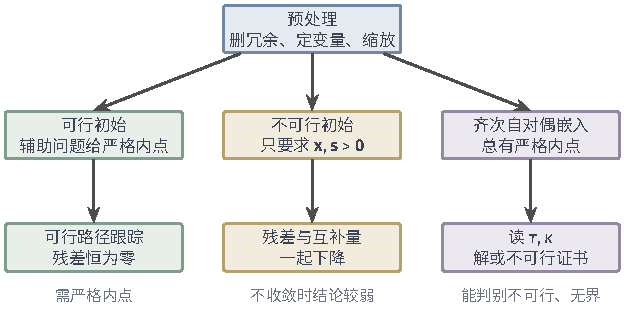
\includegraphics[width=105.738mm]{figures/05-optimization/01-linear-programming/tikz/lpipm-init-routes/figure.pdf}
  \caption{内点法起点的三条路线。预处理先去掉冗余和退化的结构。绿色路线先求严格可行点，迭代中残差恒为零；黄色路线只要求$\bm{x},\bm{s}>\bm{0}$，等式残差与互补量同时下降；紫色路线把问题嵌入一个总有严格内点的模型，由$\tau,\kappa$读出结局，并在问题不可解时给出证书。}
  \label{fig:lpipm-init-routes}
\end{BookInlineFigure}

\section{求解精度}
\label{sec:lpipm-accuracy}

内点法的迭代点永远在内部，算法只能在某一步停下来。这就需要回答：什么时候可以停，停下来的点能说明什么，以及如果需要的不是近似解而是一个基、甚至一张严格的证书，还要做什么？

\paragraph{三项残差共同决定停止}
一个点要接近最优，式~\eqref{eq:lpipm-kkt}的三组条件都要接近成立。通常用相对残差写成三条：
\begin{equation}
 \frac{\lVert\bm{A}\bm{x}-\bm{b}\rVert_2}{1+\lVert\bm{b}\rVert_2}\leq\varepsilon_{\mathrm{p}},\qquad
 \frac{\lVert\bm{A}^\top\bm{y}+\bm{s}-\bm{c}\rVert_2}{1+\lVert\bm{c}\rVert_2}\leq\varepsilon_{\mathrm{d}},\qquad
 \frac{\bm{x}^\top\bm{s}}{1+\lvert\bm{c}^\top\bm{x}\rvert}\leq\varepsilon_{\mathrm{g}}.
 \label{eq:lpipm-stop}
\end{equation}
分母里的$1$防止右端或目标恰好接近零时的除零。这些容差的意义依赖数据的尺度：把一条约束乘以$1000$，第一项的数值就改变，这和第~\ref{chap:optimization}章讨论可行性残差时指出的情况相同。

\paragraph{互补量何时是误差上界}
式~\eqref{eq:lpipm-gap-identity}的恒等式依赖两侧都可行，这时结论是干净的。

\begin{theorem}[可行点上的误差界]
\label{thm:lpipm-gap-bound}
设$\bm{x}$原始可行，$(\bm{y},\bm{s})$对偶可行。则
\begin{equation}
 0\leq\bm{c}^\top\bm{x}-p^\star\leq\bm{x}^\top\bm{s},\qquad
 0\leq d^\star-\bm{b}^\top\bm{y}\leq\bm{x}^\top\bm{s}.
 \label{eq:lpipm-gap-bound}
\end{equation}
\end{theorem}

\begin{proof}
$\bm{x}$可行给出$\bm{c}^\top\bm{x}\geq p^\star$。由弱对偶$\bm{b}^\top\bm{y}\leq d^\star\leq p^\star$，得到
\[
 \bm{c}^\top\bm{x}-p^\star\leq\bm{c}^\top\bm{x}-\bm{b}^\top\bm{y}=\bm{x}^\top\bm{s}.
\]
第二式同理，用$\bm{c}^\top\bm{x}\geq p^\star\geq d^\star$。
\end{proof}

两侧不可行时，这个界不再成立。此时
\[
 \bm{c}=\bm{A}^\top\bm{y}+\bm{s}-\bm{r}_{\mathrm{d}},\qquad\bm{b}=\bm{A}\bm{x}-\bm{r}_{\mathrm{p}}.
\]
代入目标差并整理，得到
\begin{equation}
 \bm{c}^\top\bm{x}-\bm{b}^\top\bm{y}=\bm{x}^\top\bm{s}-\bm{r}_{\mathrm{d}}^\top\bm{x}+\bm{r}_{\mathrm{p}}^\top\bm{y}.
 \label{eq:lpipm-gap-general}
\end{equation}

后两项的大小取决于残差和$\bm{x},\bm{y}$的大小。对目标误差有下面的两侧估计，它说明“残差小”换算成“目标差小”要付出什么。设$(\bm{x}^\star,\bm{y}^\star,\bm{s}^\star)$是一对最优解。

由$\bm{c}=\bm{A}^\top\bm{y}^\star+\bm{s}^\star$和$\bm{b}^\top\bm{y}^\star=p^\star$，直接计算得到
\[
 \bm{c}^\top\bm{x}-p^\star=(\bm{y}^\star)^\top\bm{r}_{\mathrm{p}}+(\bm{s}^\star)^\top\bm{x}\geq(\bm{y}^\star)^\top\bm{r}_{\mathrm{p}}.
\]
另一方面，把上面关于$\bm{c}$的表达式用到最优解$\bm{x}^\star$上，得到
\[
 p^\star=\bm{c}^\top\bm{x}^\star=\bm{b}^\top\bm{y}+\bm{s}^\top\bm{x}^\star-\bm{r}_{\mathrm{d}}^\top\bm{x}^\star.
\]
由$\bm{s}^\top\bm{x}^\star\geq0$和式~\eqref{eq:lpipm-gap-general}，得到上界。合起来就是
\begin{equation}
 (\bm{y}^\star)^\top\bm{r}_{\mathrm{p}}
 \leq\bm{c}^\top\bm{x}-p^\star
 \leq\bm{x}^\top\bm{s}+\bm{r}_{\mathrm{p}}^\top\bm{y}+\bm{r}_{\mathrm{d}}^\top(\bm{x}^\star-\bm{x}).
 \label{eq:lpipm-near-bound}
\end{equation}

这个结果的含义是，等式残差被最优解的大小放大。左端里$\bm{y}^\star$相当于影子价格：原始残差$\bm{r}_{\mathrm{p}}$相当于多用了或少用了资源，目标可以因此偏离$(\bm{y}^\star)^\top\bm{r}_{\mathrm{p}}$。所以$\bm{x}^\top\bm{s}$小并不代表目标差小，还要等式残差足够小。

图~\ref{fig:lpipm-gap-sandwich}展示了这种差别。图(a)的起点严格可行，蓝线$\bm{c}^\top\bm{x}$从上方、紫线$\bm{b}^\top\bm{y}$从下方夹住$p^\star=1$，这就是定理~\ref{thm:lpipm-gap-bound}。图(b)的起点是$\bm{x}=0.1\bm{1}$、$\bm{s}=\bm{1}$、$y=0$，等式不成立，蓝线一度在红线下方，说明此时目标值比最优值还小，并不是好事，这和第~\ref{chap:optimization}章资源分配中那个超出资源的点是同一种现象。

\begin{BookInlineFigure}
  \centering
  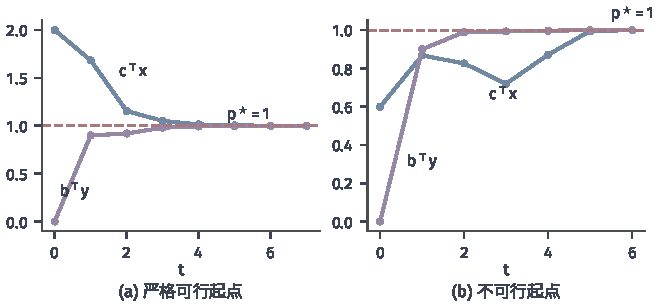
\includegraphics[width=112mm]{figures/05-optimization/01-linear-programming/matplotlib/lpipm-gap-sandwich/figure.pdf}
  \caption{原始目标（蓝）与对偶目标（紫）的夹逼，红色虚线是$p^\star=1$，$\sigma=0.3$。(a)严格可行起点，两条线从两侧夹住最优值，差距等于$\bm{x}^\top\bm{s}$。(b)不可行起点$\bm{x}=0.1\bm{1}$、$\bm{s}=\bm{1}$、$y=0$，前几轮原始目标低于最优值，原始目标甚至低于对偶目标。}
  \label{fig:lpipm-gap-sandwich}
\end{BookInlineFigure}

用图(b)的第一轮结果核对。那一点的数据是
\[
 \bm{x}\approx(0.1744,0.1521,0.1298)^\top,\qquad y=0.9,\qquad\bm{s}\approx(0.1,0.3231,0.5463)^\top,
\]
等式残差和目标值是
\[
 r_{\mathrm{p}}\approx-0.5438,\qquad\bm{r}_{\mathrm{d}}\approx(0,-0.7769,-1.5537)^\top,\qquad\bm{c}^\top\bm{x}\approx0.8678.
\]
这时$\bm{x}^\top\bm{s}\approx0.1375$是正的，但$\bm{c}^\top\bm{x}-\bm{b}^\top\bm{y}\approx-0.0322$是负的，与式~\eqref{eq:lpipm-gap-general}的右端一致。

目标误差$\bm{c}^\top\bm{x}-p^\star\approx-0.1322$落在式~\eqref{eq:lpipm-near-bound}的两端之间：左端$y^\star r_{\mathrm{p}}\approx-0.5438$，右端约为$-0.0322$。

\paragraph{近似解与精确解}
停止时得到的点满足式~\eqref{eq:lpipm-stop}，这是在给定容差和浮点运算下的结论。它和精确最优解是两回事，具体差别至少有三处。

第一，它通常不可行：$\bm{A}\bm{x}=\bm{b}$只成立到舍入误差，$\bm{x}>\bm{0}$只在严格的算术上成立。第二，它不是顶点：贯穿例第$7$轮的$x_2,x_3$是$2\times10^{-4}$和$1\times10^{-4}$，并不是零，把它们置零之后等式又不成立了。第三，浮点解的最后几位受舍入和$\bm{M}$的条件数影响，容差设得过小并不会让结果更准，反而可能使线性系统求解失败。

所以报告结果时应当把三项残差一起报告，说明容差和尺度。“求解成功”指的只是这三项达标，至于是否足够精确，要看用途。

\paragraph{基恢复}
有些用途需要一个基：要接着用单纯形法作参数分析（第~\ref{chap:simplex-method}章），要作整数规划的分支，或者需要一个顶点解。内点法不直接给出基，要从近似解转换，这一过程称为\term{基恢复}（crossover）。

做法分两阶段。先由$\hat{\bm{x}}$和$\hat{\bm{s}}$猜测哪些变量为正，例如比较$\hat{x}_i$与$\hat{s}_i$的大小，把判为零的$x_i$置零，并在其余列上修正使等式成立。然后，判为正的变量可能多于$m$个，这时沿$\bm{A}$的零空间方向移动，保持目标不变并把多余的变量逐个推到零，直到剩下的列线性无关；对偶一侧作类似的推动。最后得到一个基，用单纯形法的计算重新求出解并检查符号。

以第~\ref{sec:lpipm-central-path}节目标$\bm{c}=(0,0,1)$的例子说明。设内点法输出近似解$\hat{\bm{x}}=(0.4995,0.4995,0.001)^\top$，$\hat{\bm{s}}$的前两个分量很小，第三个分量接近$1$。比较大小后判定$x_3=0$，并修正成$(1/2,1/2,0)^\top$。

正的变量有两个，而$m=1$，还多一个。沿零空间方向$\bm{d}=(1,-1,0)^\top$移动，目标不变，走到$x_2=0$，得到顶点$(1,0,0)^\top$，基是$B=(1)$，如图~\ref{fig:lpipm-crossover}。

\begin{BookInlineFigure}
  \centering
  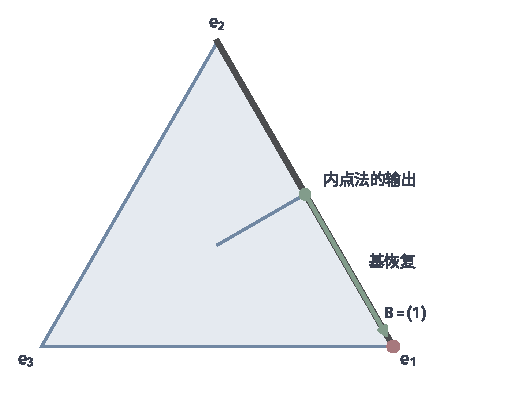
\includegraphics[width=90mm]{figures/05-optimization/01-linear-programming/matplotlib/lpipm-crossover/figure.pdf}
  \caption{基恢复的一步。目标$\bm{c}=(0,0,1)$，深灰粗线是最优边，蓝线是中心路径。内点法的输出（绿点）靠近最优边的中点，沿最优边的方向推到端点$\bm{e}_1$（红点），得到基$B=(1)$。推向$\bm{e}_2$同样得到一个最优基，所以恢复的基不唯一。}
  \label{fig:lpipm-crossover}
\end{BookInlineFigure}

用这个基作检验。$\bm{x}_B=1$，对偶是$\bm{y}=\bm{A}_B^{-\top}c_1=0$，约化成本是
\[
 \bm{s}=\bm{c}-\bm{A}^\top\bm{y}=(0,0,1)^\top\geq\bm{0},
\]
基是最优的。如果符号检验失败，从这个基继续作若干次单纯形换基。基恢复的工作量取决于$\hat{\bm{x}}$的正分量比$m$多多少，以及猜测的准确程度。已知严格互补解时恢复最优基只需多项式次运算，但实际耗时可能超过内点迭代本身。

\paragraph{精确证书}
基恢复之后得到的基和解还是浮点数算出的。如果数据是有理数，又需要严格证书，要再走一步。基矩阵$\bm{A}_B$本身是精确的，所以可以用有理数运算重新计算
\begin{equation}
 \bm{x}_B=\bm{A}_B^{-1}\bm{b},\qquad\bm{y}=\bm{A}_B^{-\top}\bm{c}_B,\qquad\bm{s}=\bm{c}-\bm{A}^\top\bm{y},
 \label{eq:lpipm-exact-check}
\end{equation}
并精确地检查$\bm{x}_B\geq\bm{0}$和$\bm{s}\geq\bm{0}$。这种检查不受任何舍入影响，通过时就是严格的最优性证明，这一点和第~\ref{chap:linear-programming}章的证书完全一致。

另一种办法是先把浮点解有理化，再验算。由Cramer法则，基本解的分母整除$\det\bm{A}_B$。两个分母都不超过$Q$的不同有理数至少相差$1/Q^2$，所以浮点解的误差只要小于$1/(2Q^2)$，分母不超过$Q$的最近有理数就只有一个，可以通过连分数求出，然后再用精确运算核对。

例如把贯穿例的约束改成$3x_1+x_2+x_3=1$，最优解是$x_1=1/3$。设内点法和基恢复给出$\hat{x}_1=0.33333341$。这里$\det\bm{A}_B=3$，分母不超过$3$的最近有理数是$1/3$。在基$B=(1)$上按式~\eqref{eq:lpipm-exact-check}作精确计算，得到
\[
 x_1=\frac13,\qquad y=\frac13,\qquad\bm{s}=\Bigl(0,\frac53,\frac83\Bigr)^\top\geq\bm{0}.
\]
这是一张可以逐项核对的最优性证书。

图~\ref{fig:lpipm-solution-pipeline}把这几个阶段连起来。算法名义上“求解完成”可以停在其中任何一个阶段，每一阶段交出的东西含义不同：近似的内部点、一个基、一个浮点最优性检验通过的基、一张严格的证书。使用结果时要分清拿到的是哪一种。

\begin{BookInlineFigure}
  \centering
  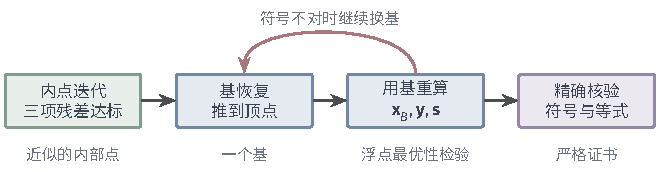
\includegraphics[width=111.739mm]{figures/05-optimization/01-linear-programming/tikz/lpipm-solution-pipeline/figure.pdf}
  \caption{从内点迭代到严格证书的各个阶段。下方灰字是每个阶段交出的结果，红色箭头表示基恢复后符号检验不通过时继续换基。}
  \label{fig:lpipm-solution-pipeline}
\end{BookInlineFigure}

\section{多项式复杂度}
\label{sec:lpipm-complexity}

单纯形法的换基次数在最坏情形下可以随维数指数增长。内点法能不能给出一个随规模温和增长的迭代次数上界？我们用最容易分析的短步路径跟踪来证明这样的界，再把它翻译成对整个算法运算量的陈述，最后指出这条界和实用规则的距离。

\paragraph{中心路径邻域}
分析的关键是不能让迭代点离路径太远，否则Newton线性化不再可靠。把“靠近路径”写成一个可以检验的条件：

\begin{definition}[中心路径的$\mathcal{N}_2$邻域]
\label{def:lpipm-neighborhood}
对$\theta\in(0,1)$，定义
\begin{equation}
 \mathcal{N}_2(\theta)=\bigl\{(\bm{x},\bm{y},\bm{s})\in\mathcal{F}^{\circ}:\lVert\bm{X}\bm{S}\bm{1}-\mu\bm{1}\rVert_2\leq\theta\mu\bigr\},
 \label{eq:lpipm-n2}
\end{equation}
其中$\mu=\bm{x}^\top\bm{s}/n$。
\end{definition}

条件说的是：把$n$个乘积看成一个向量，它偏离平均值的欧氏长度不超过平均值的$\theta$倍。中心路径上这个偏差是零。这个集合里的每个点都满足$x_is_i\geq(1-\theta)\mu>0$，所以离边界有一定的相对距离。

\paragraph{短步算法}
短步路径跟踪用可行起点，固定取单位步长，让$\mu$每轮按一个很接近$1$的比例减小：
\begin{equation}
 \sigma=1-\frac{0.4}{\sqrt{n}},\qquad\alpha=1,\qquad\theta=0.4.
 \label{eq:lpipm-short-step}
\end{equation}
这里$\sigma$必须和$\sqrt{n}$有关，直观的理由是：$\mu$的相对变化如果太大，乘积向量要移动的距离就会超出邻域。

证明的核心是控制被丢掉的二阶项$\Delta x_i\Delta s_i$。先准备一个关于向量分量乘积的引理。

\begin{lemma}[分量乘积的界]
\label{lem:lpipm-product-bound}
设$\bm{u},\bm{v}\in\mathbb{R}^n$，$\bm{u}^\top\bm{v}\geq0$。记$\bm{U}=\operatorname{diag}(\bm{u})$，$\bm{V}=\operatorname{diag}(\bm{v})$，则
\begin{equation}
 \lVert\bm{U}\bm{V}\bm{1}\rVert_2\leq2^{-3/2}\lVert\bm{u}+\bm{v}\rVert_2^2.
 \label{eq:lpipm-product-bound}
\end{equation}
\end{lemma}

\begin{proof}
把下标分成$P=\{i:u_iv_i\geq0\}$和$Q=\{i:u_iv_i<0\}$。由$\bm{u}^\top\bm{v}\geq0$，
\[
 \sum_{i\in Q}\lvert u_iv_i\rvert\leq\sum_{i\in P}u_iv_i.
\]
对$i\in P$，由$u_iv_i\leq(u_i+v_i)^2/4$，得到
\[
 \sum_{i\in P}u_iv_i\leq\frac14\sum_{i\in P}(u_i+v_i)^2\leq\frac14\lVert\bm{u}+\bm{v}\rVert_2^2.
\]
于是，用向量的$2$范数不超过$1$范数，
\[
 \lVert\bm{U}\bm{V}\bm{1}\rVert_2^2
 \leq\Bigl(\sum_{i\in P}u_iv_i\Bigr)^2+\Bigl(\sum_{i\in Q}\lvert u_iv_i\rvert\Bigr)^2
 \leq2\Bigl(\frac14\lVert\bm{u}+\bm{v}\rVert_2^2\Bigr)^2.
\]
两边开方即得。
\end{proof}

\begin{theorem}[短步路径跟踪的迭代次数]
\label{thm:lpipm-short-step}
设$(\bm{x}^{(0)},\bm{y}^{(0)},\bm{s}^{(0)})\in\mathcal{N}_2(0.4)$，按式~\eqref{eq:lpipm-newton}、\eqref{eq:lpipm-short-step}迭代。则所有迭代点都在$\mathcal{N}_2(0.4)$中，$\mu^{(t+1)}=\sigma\mu^{(t)}$，并且当
\begin{equation}
 T\geq2.5\sqrt{n}\,\log\frac{n\mu^{(0)}}{\varepsilon}
 \label{eq:lpipm-iteration-bound}
\end{equation}
时，$(\bm{x}^{(T)})^\top\bm{s}^{(T)}\leq\varepsilon$。
\end{theorem}

\begin{proof}
记当前点在$\mathcal{N}_2(\theta)$中，$\theta=0.4$，$\mu$为平均互补量。证明分四步。

\emph{第一步，二阶项的大小。}令$\bm{R}=(\bm{X}\bm{S})^{1/2}$，并定义缩放后的方向
\[
 \bm{u}=\bm{R}\bm{X}^{-1}\Delta\bm{x},\qquad\bm{v}=\bm{R}\bm{S}^{-1}\Delta\bm{s}.
\]
当前点可行，所以$\Delta\bm{x}^\top\Delta\bm{s}=0$，从而$\bm{u}^\top\bm{v}=0$。方程组第三行给出
\[
 \bm{u}+\bm{v}=\bm{R}^{-1}\bigl(\bm{S}\Delta\bm{x}+\bm{X}\Delta\bm{s}\bigr)=\bm{R}^{-1}\bigl(\sigma\mu\bm{1}-\bm{X}\bm{S}\bm{1}\bigr).
\]
由引理~\ref{lem:lpipm-product-bound}，注意到$\bm{U}\bm{V}\bm{1}=\Delta\bm{X}\Delta\bm{S}\bm{1}$，以及$\bm{R}^{-2}$的对角元不超过$1/((1-\theta)\mu)$，得到
\[
 \lVert\Delta\bm{X}\Delta\bm{S}\bm{1}\rVert_2\leq\frac{2^{-3/2}}{(1-\theta)\mu}\lVert\sigma\mu\bm{1}-\bm{X}\bm{S}\bm{1}\rVert_2^2.
\]

\emph{第二步，计算右端。}把$\sigma\mu\bm{1}-\bm{X}\bm{S}\bm{1}$写成$(\mu\bm{1}-\bm{X}\bm{S}\bm{1})-(1-\sigma)\mu\bm{1}$。两部分正交，因为$\bm{X}\bm{S}\bm{1}-\mu\bm{1}$的分量之和是$n\mu-n\mu=0$。由勾股定理和邻域条件，
\[
 \lVert\sigma\mu\bm{1}-\bm{X}\bm{S}\bm{1}\rVert_2^2\leq\theta^2\mu^2+(1-\sigma)^2n\mu^2.
\]
代入$\theta=0.4$与$(1-\sigma)^2n=0.16$，结合上一步，得到
\[
 \lVert\Delta\bm{X}\Delta\bm{S}\bm{1}\rVert_2\leq\frac{0.32}{2^{3/2}\times0.6}\,\mu<0.19\,\mu.
\]

\emph{第三步，新点仍在邻域内。}对$\alpha\in[0,1]$，记$\bm{x}(\alpha)=\bm{x}+\alpha\Delta\bm{x}$，$\bm{s}(\alpha)$同理。由第三行，
\[
 x_i(\alpha)s_i(\alpha)=(1-\alpha)x_is_i+\alpha\sigma\mu+\alpha^2\Delta x_i\Delta s_i.
\]
前两项之和不小于$\min\{(1-\theta)\mu,\sigma\mu\}\geq0.6\mu$（$n\geq1$时$\sigma\geq0.6$），第三项的绝对值不超过$0.19\mu$，所以$x_i(\alpha)s_i(\alpha)>0$。乘积从正数出发一直为正，$x_i(\alpha)$和$s_i(\alpha)$就不能变号，因此$\bm{x}^+,\bm{s}^+>\bm{0}$。

$\Delta\bm{x}^\top\Delta\bm{s}=0$说明$\mu^+=\sigma\mu$。$\alpha=1$时，上面的展开给出$x_i^+s_i^+-\sigma\mu=\Delta x_i\Delta s_i$，于是
\[
 \lVert\bm{X}^+\bm{S}^+\bm{1}-\mu^+\bm{1}\rVert_2<0.19\,\mu\leq0.4\,\sigma\mu=\theta\mu^+,
\]
最后一步用到$0.4\sigma\geq0.24$。等式约束由线性性保持，所以新点在$\mathcal{N}_2(0.4)$中。

\emph{第四步，计数。}由上面的结论，$n\mu^{(T)}=n\sigma^T\mu^{(0)}$。利用$\log(1-\beta)\leq-\beta$，只要式~\eqref{eq:lpipm-iteration-bound}成立，就有
\[
 n\mu^{(T)}\leq n\mu^{(0)}\exp\Bigl(-\frac{0.4\,T}{\sqrt{n}}\Bigr)\leq\varepsilon.\qedhere
\]
\end{proof}

这个定理的结构可以这样概括：$\theta$保证Newton步的二阶项足够小，$\sigma$的取法让一步能被邻域容纳，两者的相容性来自$\sqrt{n}$这个因子。由于$(1-\sigma)^2n$要固定，每步减少的比例只能是$1/\sqrt{n}$量级，这就是迭代次数含$\sqrt{n}$的原因。

以贯穿例验证。从中心点$\bm{x}^{(0)}=(6/11,3/11,2/11)^\top$、$y^{(0)}=0$出发，$n=3$，$\sigma=1-0.4/\sqrt{3}\approx0.7691$，起点和前两轮的$\mu$是$0.5455$、$0.4195$、$0.3226$，每轮都乘以$\sigma$。全程相对偏差的最大值约为$0.045$，远小于$0.4$。

取$\varepsilon=10^{-3}$，式~\eqref{eq:lpipm-iteration-bound}给出的上界是
\[
 2.5\sqrt{3}\,\log\frac{18/11}{10^{-3}}\approx32.04,
\]
实际用了$29$轮。短步规则的实际轮数几乎就是理论值，因为$\sigma$是预先固定的。作为对照，第~\ref{sec:lpipm-path-following}节同一个问题用预测—校正把互补量降到$10^{-3}$以下只需$4$轮。

\paragraph{从迭代次数到运算量}
式~\eqref{eq:lpipm-iteration-bound}只计迭代次数。要说“线性规划可以在多项式时间内求解”，还要计入每一轮的代价和数字的长度。整个结论由下面三部分拼成。

第一是每轮的算术运算量：解一个$m\times m$的稠密方程组，需要$O(n^3)$次算术运算（$m\leq n$）。第二是迭代次数中的$\log(n\mu^{(0)}/\varepsilon)$，要说清起点和精度是多少。

第三部分是输入的位长。设数据全部是整数，写出整个问题需要$L$个二进制位，这里$L$至少是$m,n$和各系数位数的总和。可以证明两件事：存在满足定理条件的起点，其$\mu^{(0)}$不超过$2^{O(L)}$，这类起点由第~\ref{sec:lpipm-initial-point}节的嵌入构造给出；只要把间隙降到$2^{-O(L)}$以下，由于有理顶点的分母有界，就可以把近似解精确地修整成最优基。

把这三部分合起来，得到迭代次数$O(\sqrt{n}L)$，算术运算总量$O(n^{3.5}L)$，运算中只需保留$O(L)$位的精度，总的二进制运算量是$L$和$n$的多项式。严格的推导要逐项跟踪精度和起点，篇幅较长，读者可查阅专著\scite{math-bertsimas1997linear}。

这里“多项式”的含义要说准。上面的界依赖$L$，也就是系数的位数，所以这是位模型下的多项式时间，又称弱多项式。是否存在迭代次数只依赖$m,n$、不依赖系数位长的线性规划算法，至今仍是公开问题。内点法的$\log(1/\varepsilon)$项在这里起作用：想要精确解，就需要把精度推到由$L$决定的程度。

\paragraph{理论规则与实用规则}
短步规则的上界最好，实际却很慢：它每轮只减小约$0.4/\sqrt{n}$，从不利用可以走更远的情况。放宽邻域能让步子变大。定义单侧邻域
\begin{equation}
 \mathcal{N}_{-\infty}(\gamma)=\bigl\{(\bm{x},\bm{y},\bm{s})\in\mathcal{F}^{\circ}:x_is_i\geq\gamma\mu,\ i=1,\ldots,n\bigr\},\quad\gamma\in(0,1).
 \label{eq:lpipm-n-inf}
\end{equation}
$\gamma$很小时，几乎只要求每个乘积不要低于平均值太多。图~\ref{fig:lpipm-neighborhoods}(a)是$n=2$时两种邻域在乘积平面上的形状：$\mathcal{N}_2$是窄条，$\mathcal{N}_{-\infty}$几乎占满整个象限。

\begin{BookInlineFigure}
  \centering
  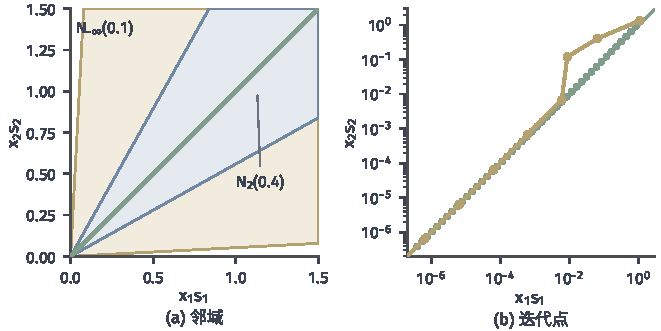
\includegraphics[width=112mm]{figures/05-optimization/01-linear-programming/matplotlib/lpipm-neighborhoods/figure.pdf}
  \caption{$n=2$时中心路径的邻域，横纵轴是两个乘积$x_1s_1,x_2s_2$，绿色对角线是中心路径。(a)蓝色是$\mathcal{N}_2(0.4)$，黄色是$\mathcal{N}_{-\infty}(0.1)$。(b)问题$\min x_1+2x_2$、$x_1+x_2=1$上的迭代点，对数坐标。绿点是短步规则，黄点是$\sigma=0.1$的长步规则，长步规则离路径更远，点数少得多。}
  \label{fig:lpipm-neighborhoods}
\end{BookInlineFigure}

在$\mathcal{N}_{-\infty}(\gamma)$上，每轮取较小的$\sigma$，再沿方向走到将要离开邻域为止，称为长步路径跟踪。它的理论上界是$O(n\log(1/\varepsilon))$，比短步的$O(\sqrt{n}\log(1/\varepsilon))$差，实际表现却远好于短步。

第~\ref{sec:lpipm-path-following}节的预测—校正规则则按式~\eqref{eq:lpipm-sigma-rule}自适应地选$\sigma$，加上二阶校正。按通常的写法，它没有多项式的迭代次数保证，但它是大规模求解器的常用方案。

图~\ref{fig:lpipm-iteration-growth}是随机线性规划上的迭代次数。每个问题都从同一个中心点出发，要求$\mu\leq10^{-6}$。短步规则的轮数紧贴理论值，随$\sqrt{n}$增长，$n=1000$时超过一千轮。长步规则和预测—校正增长得慢得多，$n=1000$时只需$23$轮和$12$轮。

\begin{BookInlineFigure}
  \centering
  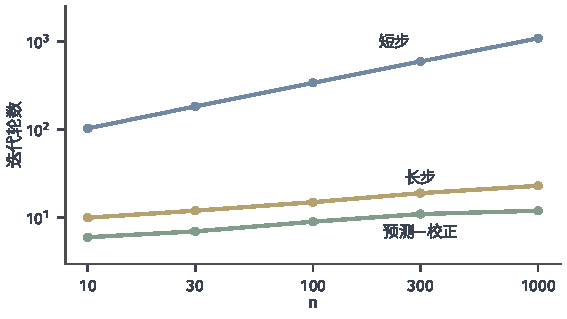
\includegraphics[width=96mm]{figures/05-optimization/01-linear-programming/matplotlib/lpipm-iteration-growth/figure.pdf}
  \caption{随机稠密线性规划上三种规则的迭代轮数，$m=n/2$，对数坐标，起点$\bm{x}=\bm{s}=\bm{1}$是中心点，停止条件$\mu\leq10^{-6}$。蓝线是短步规则，黄线是长步规则（$\sigma=0.1$、$\gamma=10^{-3}$），绿线是预测—校正。每个$n$只运行一个固定种子的实例，用来展示量级而不是平均表现。}
  \label{fig:lpipm-iteration-growth}
\end{BookInlineFigure}

表~\ref{tab:lpipm-rules}把三者放在一起。理论界最好的规则不是实践中最快的规则，这个差距是内点法的一个基本事实。

\begin{BookInlineTable}
  \centering
  \begin{tabular}{@{}llll@{}}
    \toprule
    规则 & 邻域 & 迭代上界 & 实践表现\\
    \midrule
    短步 & $\mathcal{N}_2(0.4)$ & $O(\sqrt{n}\log(1/\varepsilon))$ & 接近理论值，很慢\\
    长步 & $\mathcal{N}_{-\infty}(\gamma)$ & $O(n\log(1/\varepsilon))$ & 轮数少\\
    预测—校正 & 无固定邻域 & 无一般保证 & 通常最少\\
    \bottomrule
  \end{tabular}
  \caption{三种路径跟踪规则的比较。上界针对可行起点；预测—校正指式~\eqref{eq:lpipm-sigma-rule}的常用写法，加上保护措施的变体可以恢复多项式界。}
  \label{tab:lpipm-rules}
\end{BookInlineTable}

\paragraph{历史上的位置}
线性规划的多项式可解性最早不是由内点法确立的。1979年，Khachiyan用椭球法证明了线性规划可以在多项式时间内求解，这个方法每步用一个椭球包住可能的解集，并不断缩小椭球。它在理论上解决了问题，实际计算却很慢。

1984年Karmarkar提出的算法同样具有多项式复杂度，并且在实践中有竞争力，随后的工作发展出本章的原始—对偶路径跟踪。这段历史可以帮助分清两件事：多项式界回答“最坏情形下随规模怎样增长”，实际快慢还取决于常数、结构和实现。

\section{单纯形法与内点法的比较}
\label{sec:lpipm-comparison}

现在两种算法都有了。于是要问：面对一个具体的线性规划，两者各需要做什么、各能交出什么？我们先在同一个工厂问题上把它们并排算一遍，再按稀疏性、内存、退化和再求解几个方面对比。

\paragraph{同一个问题上的两种计算}
工厂问题的标准型是第~\ref{chap:simplex-method}章的数据，$m=3$，$n=5$，最优解是$(4,2,0,0,1)^\top$，最优利润$26$，对偶最优解$\bm{y}^\star=(-2,-1,0)^\top$。单纯形法从基$(3,4,5)$出发，经过$(0,3)$、$(2,3)$，$3$次换基到达最优顶点，每次换基求解一个$3\times3$的基矩阵方程组。

内点法取严格可行起点
\[
 \bm{x}^{(0)}=(1,1,5,7,2)^\top,\qquad\bm{y}^{(0)}=(-3,-3,-3)^\top,\qquad\bm{s}^{(0)}=(5,7,3,3,3)^\top,
\]
这里$\bm{s}^{(0)}=\bm{c}-\bm{A}^\top\bm{y}^{(0)}$，$\mu^{(0)}=10.8$。第一轮的正规矩阵是
\[
 \bm{M}=\bm{A}\bm{D}\bm{A}^\top\approx
 \begin{bmatrix}2.4381&0.6857&0.2857\\0.6857&3.2762&0.1429\\0.2857&0.1429&0.8095\end{bmatrix}.
\]

两种算法都在解$3\times3$的对称或非对称方程组，表面上规模一样，含义却不同。基矩阵只用$\bm{A}$的$3$列，换基时只变一列；$\bm{M}$用到全部$5$列，每轮的数值都变，但元素的稀疏结构不变。

用预测—校正（$\eta=0.99$），$6$轮后互补量从$54$降到约$1.2\times10^{-7}$，点在$4$位小数上就是$(4,2,0,0,1)^\top$。

图~\ref{fig:lpipm-factory-run}把这两个过程画在一起。单纯形法的每一步都站在顶点上，利润单调上升，$3$步后得到精确解。内点法的头几轮就穿过内部接近最优点，第$3$轮已到$25.95$，但此后每轮只是把小数位往后推，点始终不是顶点。

\begin{BookInlineFigure}
  \centering
  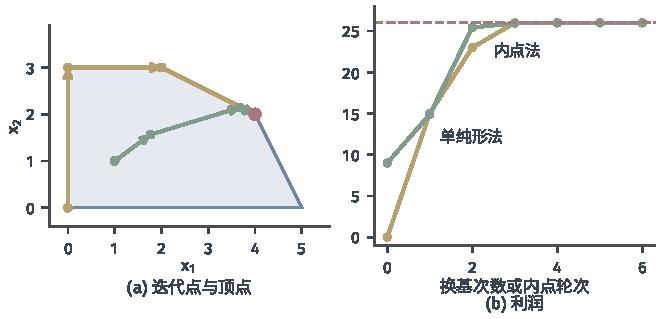
\includegraphics[width=112mm]{figures/05-optimization/01-linear-programming/matplotlib/lpipm-factory-run/figure.pdf}
  \caption{工厂问题上的两种算法。(a)可行域上，黄色是单纯形法的顶点序列，绿色是内点法的前几个迭代点，红点是最优顶点$(4,2)$。(b)利润随迭代的变化，黄线是单纯形法的换基次数，绿线是内点法的轮次，红色虚线是最优值$26$。单纯形法的横轴单位是一次换基，内点法的单位是一次分解$\bm{M}$，两者的代价不同，不能只比轮次。}
  \label{fig:lpipm-factory-run}
\end{BookInlineFigure}

\paragraph{稀疏存储与分解填充}
大规模线性规划的矩阵$\bm{A}$几乎都是稀疏的，这时代价取决于分解时产生多少新的非零元（填充）。两种算法的填充模式不同。

单纯形法分解基矩阵，用LU分解并在换基时更新，只涉及$m$列。内点法分解$\bm{A}\bm{D}\bm{A}^\top$，它的第$(i,k)$个元素非零，当且仅当存在一列在第$i$行和第$k$行都非零。于是只要$\bm{A}$有一列稠密，$\bm{M}$就整个稠密。

图~\ref{fig:lpipm-sparsity}是一个例子：$\bm{A}$是$40\times80$的稀疏矩阵，每列只有两个非零元，再加上一个稠密列。整个$\bm{A}$只有$198$个非零元，$\bm{M}$却有全部$1600$个；去掉那一列后，$\bm{M}$只有$196$个非零元。实现中会把稠密列单独分离出来，用矩阵求逆引理处理，但这需要额外的数值稳定措施。

\begin{BookInlineFigure}
  \centering
  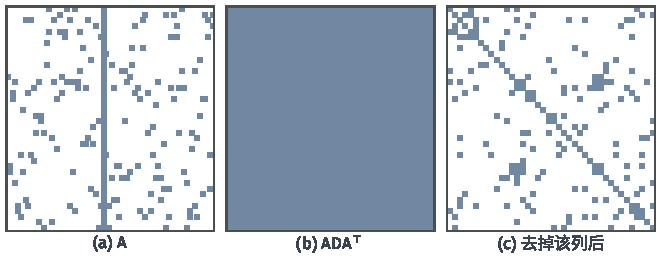
\includegraphics[width=112mm]{figures/05-optimization/01-linear-programming/matplotlib/lpipm-sparsity/figure.pdf}
  \caption{一个稠密列的影响，蓝色方块表示非零元。(a)$40\times80$的稀疏矩阵$\bm{A}$，其中一列稠密。(b)正规矩阵$\bm{A}\bm{D}\bm{A}^\top$完全稠密。(c)去掉该列后的$\bm{A}\bm{D}\bm{A}^\top$仍然稀疏。}
  \label{fig:lpipm-sparsity}
\end{BookInlineFigure}

\paragraph{内存}
内点法每轮要存$\bm{M}$的Cholesky因子，内存由填充决定，并且在整个求解期间都要占用这么多。单纯形法只存基的LU因子，通常比前者小，但可能需要很多次换基。所以问题规模增大时，内点法更容易受内存限制，单纯形法更容易受迭代次数限制，具体哪个先成为瓶颈取决于矩阵结构。

\paragraph{退化与数值性质}
第~\ref{chap:simplex-method}章说明，退化时单纯形法可能原地换基，需要反循环规则。内点法从不访问顶点，路径本身不受退化的基影响，第$t$轮的$\bm{D}$只和当前点有关，因此没有“卡在同一顶点”的现象。

内点法的麻烦在别处。$\bm{D}$的对角元是$x_i/s_i$，随迭代趋于两个极端：最优解中为正的变量对应的元素趋于$+\infty$，为零的变量对应的元素趋于$0$。图~\ref{fig:lpipm-scaling-spread}(a)显示，工厂问题最后几轮对角元的比值已超过$10^{20}$。

\begin{BookInlineFigure}
  \centering
  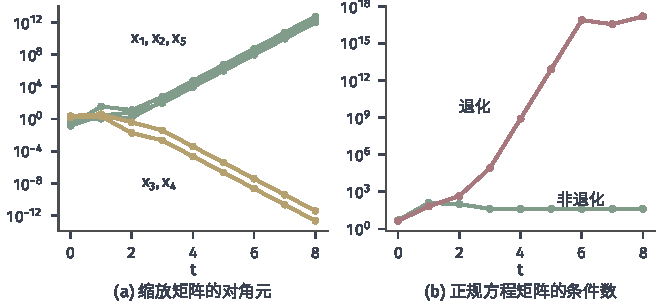
\includegraphics[width=112mm]{figures/05-optimization/01-linear-programming/matplotlib/lpipm-scaling-spread/figure.pdf}
  \caption{缩放矩阵与条件数的变化，预测—校正，$\eta=0.99$。(a)工厂问题中$D_{ii}=x_i/s_i$随轮次的变化，绿线对应最优解中为正的$x_1,x_2,x_5$，黄线对应为零的$x_3,x_4$。(b)$\bm{M}=\bm{A}\bm{D}\bm{A}^\top$的$2$范数条件数：绿线是非退化的工厂问题，红线是再加一条约束$x_1+x_2\leq6$使最优顶点退化的情形。}
  \label{fig:lpipm-scaling-spread}
\end{BookInlineFigure}

这种悬殊看起来很危险，影响却取决于问题的结构。图~\ref{fig:lpipm-scaling-spread}(b)的绿线说明，非退化时$\bm{M}$由三个正的基变量主导，它们的$D_{ii}$同步增大，条件数稳定在约$41$。红线是最优顶点退化的情形，正变量少于$m$个，$\bm{M}$趋于奇异，条件数涨到$10^{16}$以上。

大的条件数并不直接意味着算出的方向没用：误差往往落在对后续更新影响不大的子空间里，这是内点法在实践中比条件数预示的更稳健的原因，但这需要专门的误差分析，读者可查阅专著\scite{math-nocedal2006numerical}。求解器还要辅以正则化和迭代精化。最终都应当检查残差，不能只凭条件数判断。

\paragraph{基与再求解}
单纯形法返回一个基，这使很多后续工作很方便：约束或目标有微小改变时，从原来的基接着做，往往几次换基就够（第~\ref{chap:simplex-method}章的对偶单纯形法）；固定基的参数分析可以直接读出结论成立的范围。

内点法也返回对偶信息，这些$\bm{y}$和$\bm{s}$的值可以当作影子价格用，但结果是最优面中央的一个点，解不唯一时它和某个基给出的对偶解并不相同。需要基时要做上一节的基恢复。

内点法的热启动也比较困难。上一次的解贴近边界，某些$x_i$或$s_i$接近零，从这里出发的步长通常很短，反而不如重新开始。因此在分支限界这类需要大量相关求解的场景中，单纯形法更占优势，这也是两种方法长期并存的原因之一。

\paragraph{速度取决于问题和实现}
两种算法都不总是更快。一般而言，内点法在规模很大且$\bm{M}$稀疏时往往轮数少、速度快，单纯形法在$\bm{M}$稠密或需要反复热启动时更有优势。这只是经验性的倾向，具体结果要看矩阵结构、预处理和实现水平，求解器通常提供两者甚至并行运行。

表~\ref{tab:lpipm-compare}总结了本节的对比。

\begin{table*}[!htbp]
  \centering
  \begin{tabular}{@{}lll@{}}
    \toprule
    方面 & 单纯形法 & 内点法\\
    \midrule
    每步的工作 & 解基矩阵方程，换一列 & 分解$\bm{A}\bm{D}\bm{A}^\top$，全部列参与\\
    迭代次数 & 随结构变化，最坏情形指数 & 通常很少，短步规则有$O(\sqrt{n}\log(1/\varepsilon))$的界\\
    稀疏结构 & 基的LU因子，变化较小 & 稠密列会使$\bm{M}$稠密，需特殊处理\\
    内存 & 通常较小 & 由Cholesky填充决定，通常较大\\
    退化 & 可能原地换基，需反循环规则 & 不停滞，但$\bm{M}$可能病态\\
    交出的结果 & 基、顶点解、对偶解 & 内部的近似点和对偶量，需要基时另作恢复\\
    再求解 & 从旧基热启动较容易 & 从旧解热启动较困难\\
    \bottomrule
  \end{tabular}
  \caption{单纯形法与内点法的对比。各项是对典型情形的概括，速度结论取决于问题结构和实现。无论用哪种方法，浮点实现都要检验可行性和最优性。}
  \label{tab:lpipm-compare}
\end{table*}

\section{本章小结}
\label{sec:lpipm-summary}

本章开头问：能不能不贴着边走，从可行域的内部穿过去？答案是把互补松弛$x_is_i=0$放宽成$x_is_i=\mu$。原始和对偶都有严格可行点时，这组方程对每个$\mu>0$有唯一解，解连成中心路径，沿路径的对偶间隙恰好是$n\mu$。路径的极限是一对严格互补的最优解，落在最优面的解析中心，解不唯一时并不是顶点。

沿路径前进靠Newton法。线性化$x_is_i=\sigma\mu$得到一个由原始残差、对偶残差和互补残差驱动的线性方程组，消元后只需解$m\times m$的对称正定方程$\bm{A}\bm{D}\bm{A}^\top\Delta\bm{y}=\bm{h}$。到边界的比例规则保持$\bm{x},\bm{s}>\bm{0}$，$\sigma$在减小互补量和靠近中心之间折中，预测—校正用一次试算选定$\sigma$并补偿二阶项，两次求解共用一次分解。

这些步骤合起来是一个完整的求解过程。起点可以严格可行，也可以只要求正性，让等式残差和互补量一起下降；需要判别不可行或无界时，用预处理和齐次自对偶嵌入。停止时要同时看三项残差，只有在原始、对偶都可行时，$\bm{x}^\top\bm{s}$才是目标误差的上界，否则还要计入等式残差被最优解放大的部分。

交付的结果有几个层次，它们的含义不同：浮点容差下的近似解，基恢复之后的基，用精确算术核对过的证书。理论方面，短步路径跟踪的迭代次数不超过$O(\sqrt{n}\log(n\mu^{(0)}/\varepsilon))$，配合起点构造和位长分析得到线性规划的多项式算法；椭球法更早建立了这一可解性。理论规则和实用的预测—校正之间有明显差距，不能把后者的经验速度当作定理。

选择算法时，单纯形法便于热启动、返回基，适合反复求解和灵敏度分析；内点法迭代次数少，适合大规模稀疏问题，但对$\bm{A}\bm{D}\bm{A}^\top$的填充敏感，需要基时要另作恢复。两者都需要在最后检验可行性和最优性。

路径跟踪的思路并不限于线性规划。当约束是一般的光滑函数或锥时，障碍和扰动互补仍然可用，但方程不再是双线性的，Newton系统含有Hessian和Jacobian的变化，严格内点、初值和停止证书都有新的条件，这些由第~\ref{chap:nonlinear-interior-point}章展开。


